\section{Техническое описание}
\subsection{День 1. 05.08.2022\\
Пл. Имандра -- р. Гольцовка -- руч. Меридиональный -- пер. Юмъекорр (н/к, 700 м) -- руч. Юмъекорруай}
\begin{tabular}{l p{12cm}}
\hline
Пройдено: & 18.05 км\\
Набор/сброс высоты: & 869/711 м\\
Время в пути: & 9:15\\
ЧХВ: & 6:20\\
Метеоусловия: & Днем --- солнечно. Вечером --- дождь.\\
\hline
\end{tabular}

Подъём в 6:00.
В 7:44 электричкой из Апатит отправились на станцию Имандра. В 8:24, ровно по расписанию, прибыли. Облачно, с прояснениями.

На станции созваниваемся с МЧС, отправляем sms-сообщения координатору от МКК и нашему координатору.
Подгоняем снаряжение, включаем GPS-навигаторы, делаем стартовые фотографии (рис. \ref{fig1:1}).

На маршрут выходим в 8:50. Из посёлка ст. Имандра к ст. Хибины ведёт грунтовая дорога, почти сразу она разделяется.
Выбираем ту её ветку, которая идёт вдоль железнодорожных путей до пересечения с р. Гольцовкой.
Рядом с железнодорожным мостом подвесной мост (рис. \ref{fig1:2}), попасть на тот берег можно по любому из них.
Что касается автомобилей, то предполагается что они пересекают реку по броду, но вид этого брода вызывает сомнения
в возможности сделать это на легковом автомобиле без шноркеля. Мы же выбираем подвесной мост и по одному переходим.

9:25 За мостом поворачиваем на восток, идём вдоль реки. Дорога --- лесная тропа, по пересечённой местности.
Вверх-вниз, то рядом с рекой, то отходим метров на 400. Тропа часто разветвляется, ответвления расходятся-сходятся;
выбираем на глаз удобные. Много стоянок.

11:13 Слияние руч. Меридионального и руч. Маннепахк, образующих р. Гольцовку. Много туристов на стоянках.
Нам вверх по руч. Меридиональному. На другую сторону ручья пока не переходим, идём по левому берегу.
На карте тропы нет, но по факту она есть. Идём пока не доходим до скал. Далее идти сомнительно,
поэтому переходим на другой берег. Тропа здесь, конечно, более натоптанная, лучше было сразу идти по ней.

Чуть-чуть проходим: на берегу травянистая поляна, простой спуск к воде, тропка по которой все идут вдалеке.
Становимся на обед, 13:19. Погода солнечная, плывут облачка, +25$\tccentigrade$.

14:49 Трогаемся к перевалу, идти недалеко. Пара поворотов ручья --- и открывается подъём на перевал (рис. \ref{fig1:3}).
Вдали дорога упирается в цирк.

Опять переходим основной поток. С нашего перевала спускается приток Меридионального. Начинаем подъём,
идём с левой стороны притока (рис. \ref{fig1:4}). Хорошо различимая тропа. Сама дорожка --- мелкая сыпуха, кругом --- слой почвы,
покрытый мхом, лежат отдельные средние камни.

Характерная V-образная форма перевала, на которую все ссылаются и приводят фотографии, со стороны Меридионального
не видна до самого перевала (рис. \ref{fig1:5}), из долины Меридионального тоже не видна
(разве что, может быть, с противоположного склона долины ручья, но мы туда не поднимались).

До перевала от Меридионального доходим за полчаса. Перевал состоит из нескольких камер, заполненных средними камнями;
в одной из камер снежник. Хорошо видно оз. Большая Имандра (рис. \ref{fig1:6}).
Фотографируемся (рис. \ref{fig1:7}), съедаем шоколадку,
снимаем записку \enquote{группы Геныча} от 04.08.2022 (рис. \ref{fig:zapiski1}), оставляем свою.

16:46 Начинаем спуск. Тропа на спуске --- сыпуха и средние камни. Куда спускаться понятно.
Хорошо видна V-образность перевала, особенно издали (рис. \ref{fig1:8}). Ближе к перевалу V-образность иногда скрывается склонами,
поэтому при подъёме с запада нужно быть внимательнее, чтобы не уйти не туда, например, в пер. Юмъекорр боковой.

18:01 Выбрали место для ночёвки. Стали чуть выше впадения ручья со стороны ущ. Аку-Аку в руч. Юмъекорруай
(на самом слиянии стоянки были заняты). Почти сразу пошёл дождь, закончился около 20, далее накрапывал,
в 21 температура около +20$\tccentigrade$.

Отбой 22:00.

\begin{figure}
    \centering
    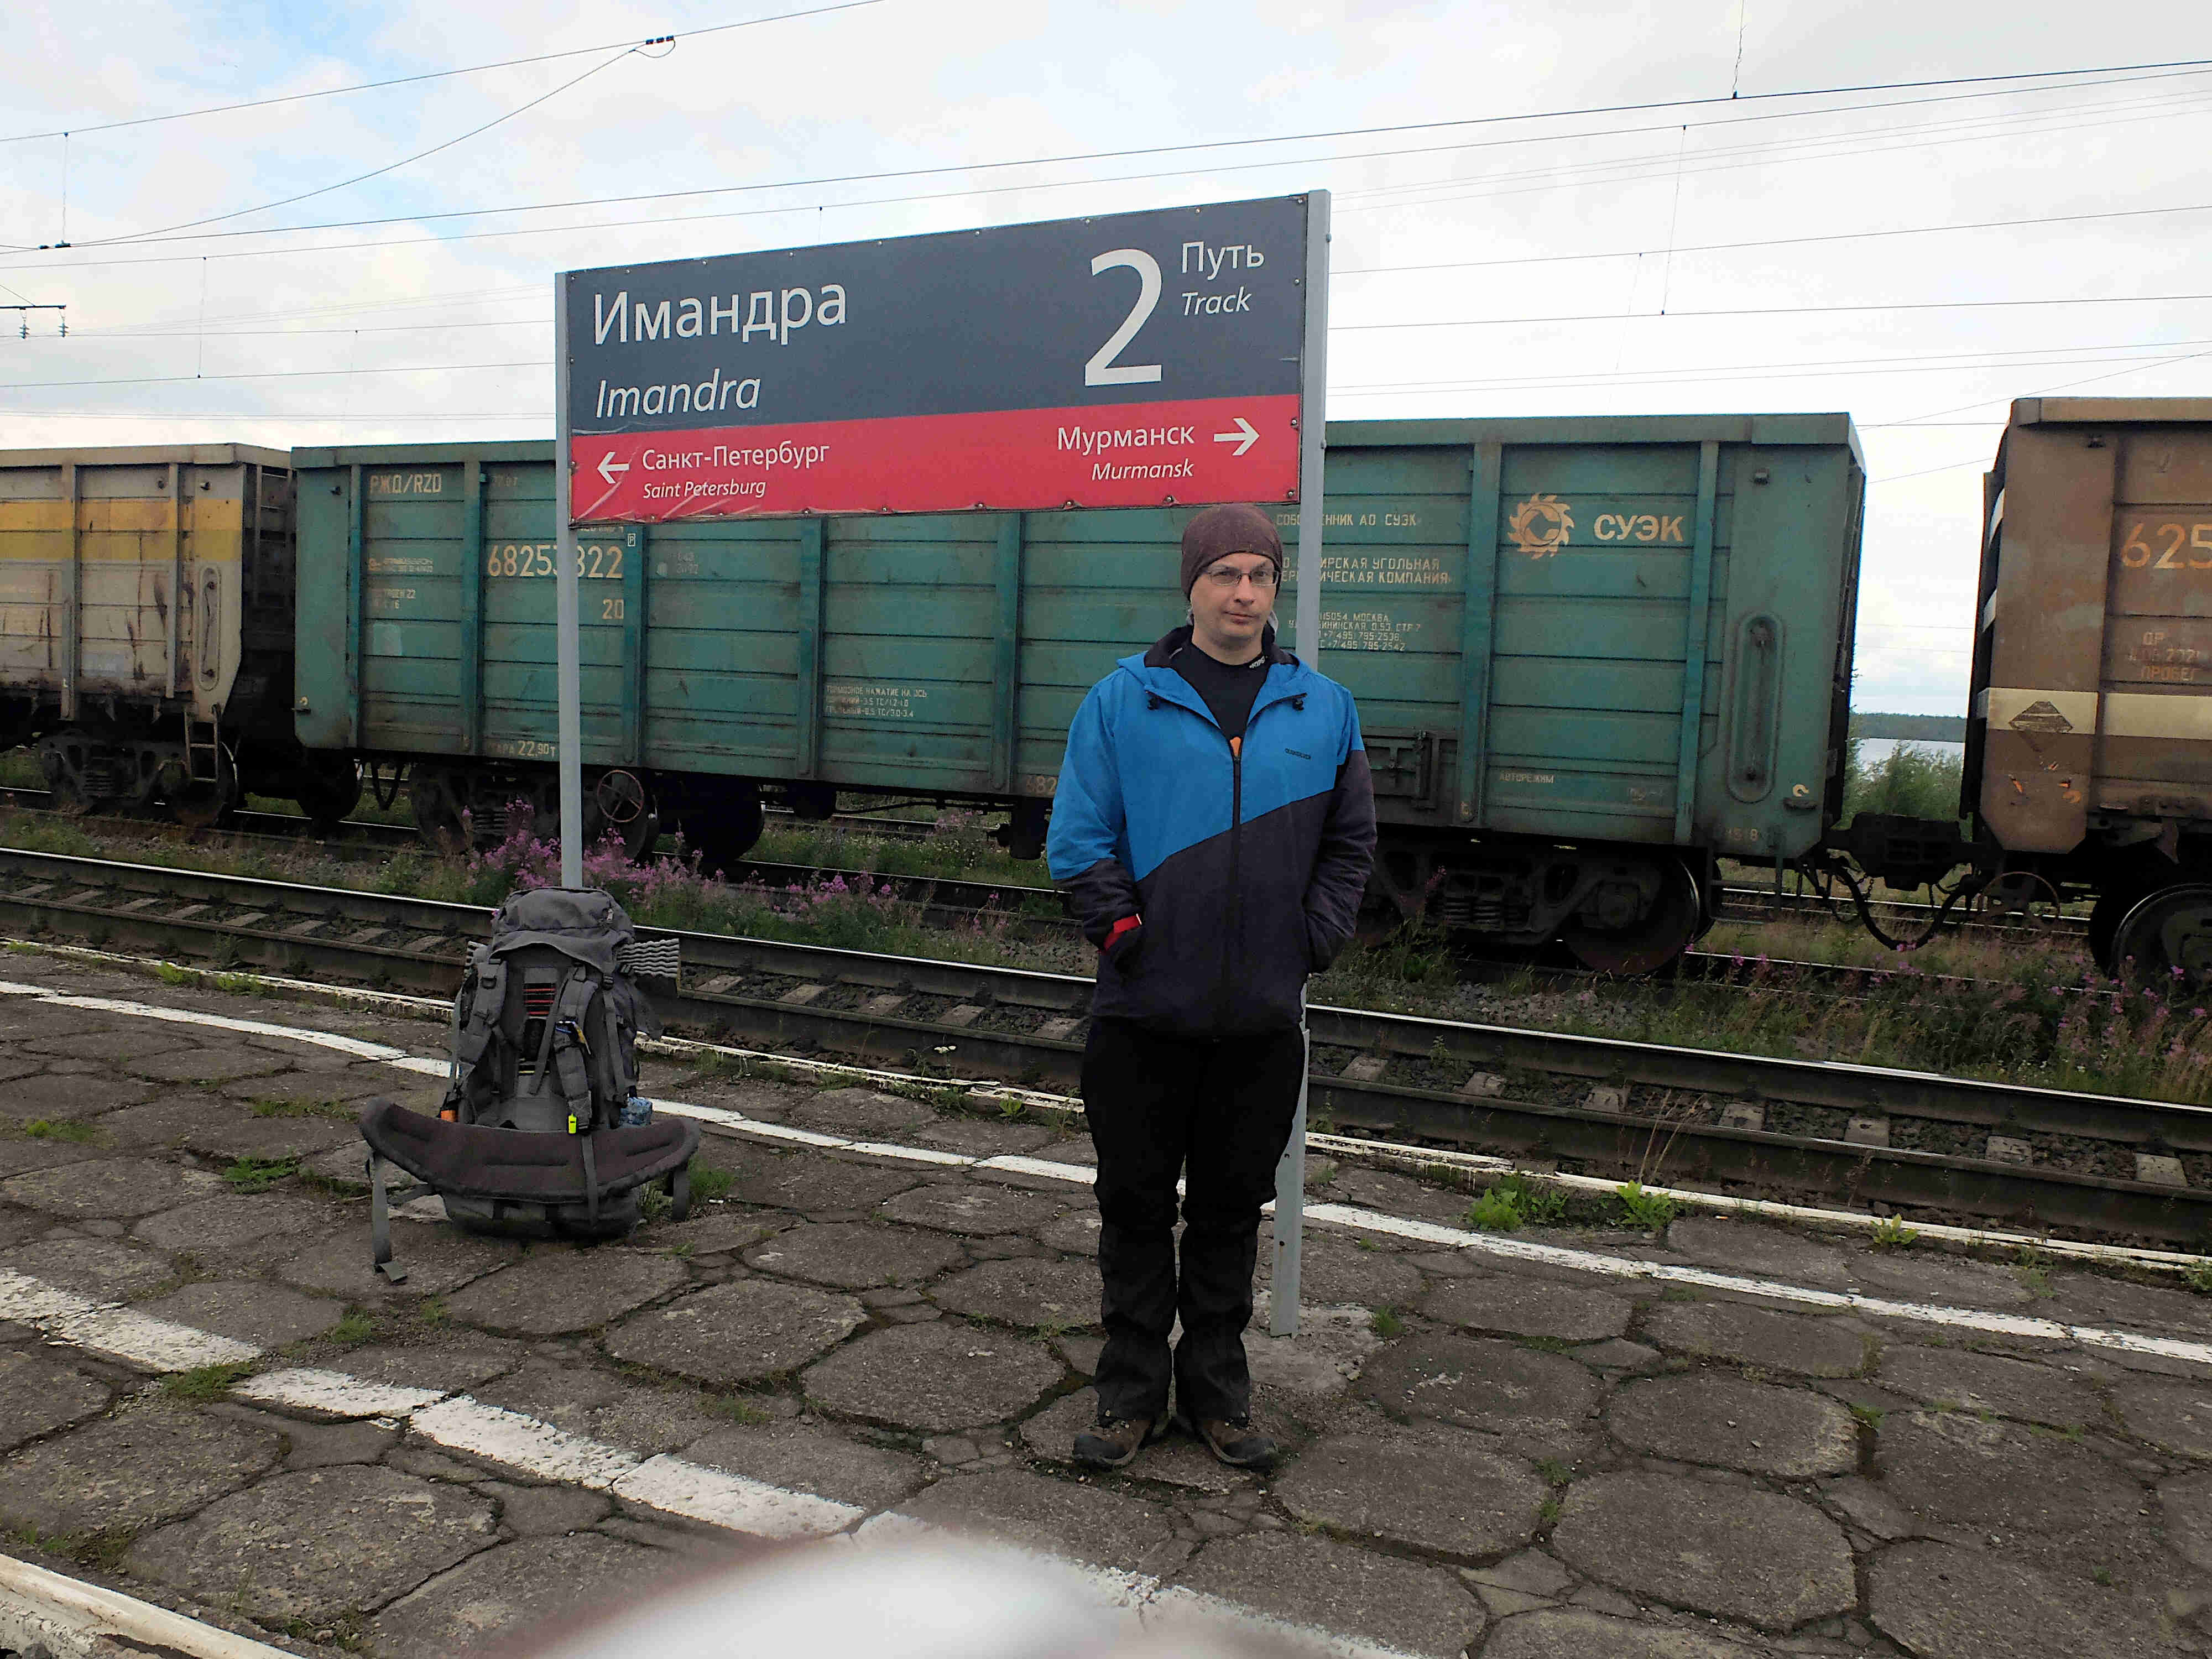
\includegraphics[width=14cm]{foto/Лица/mordas1_1.JPG}
    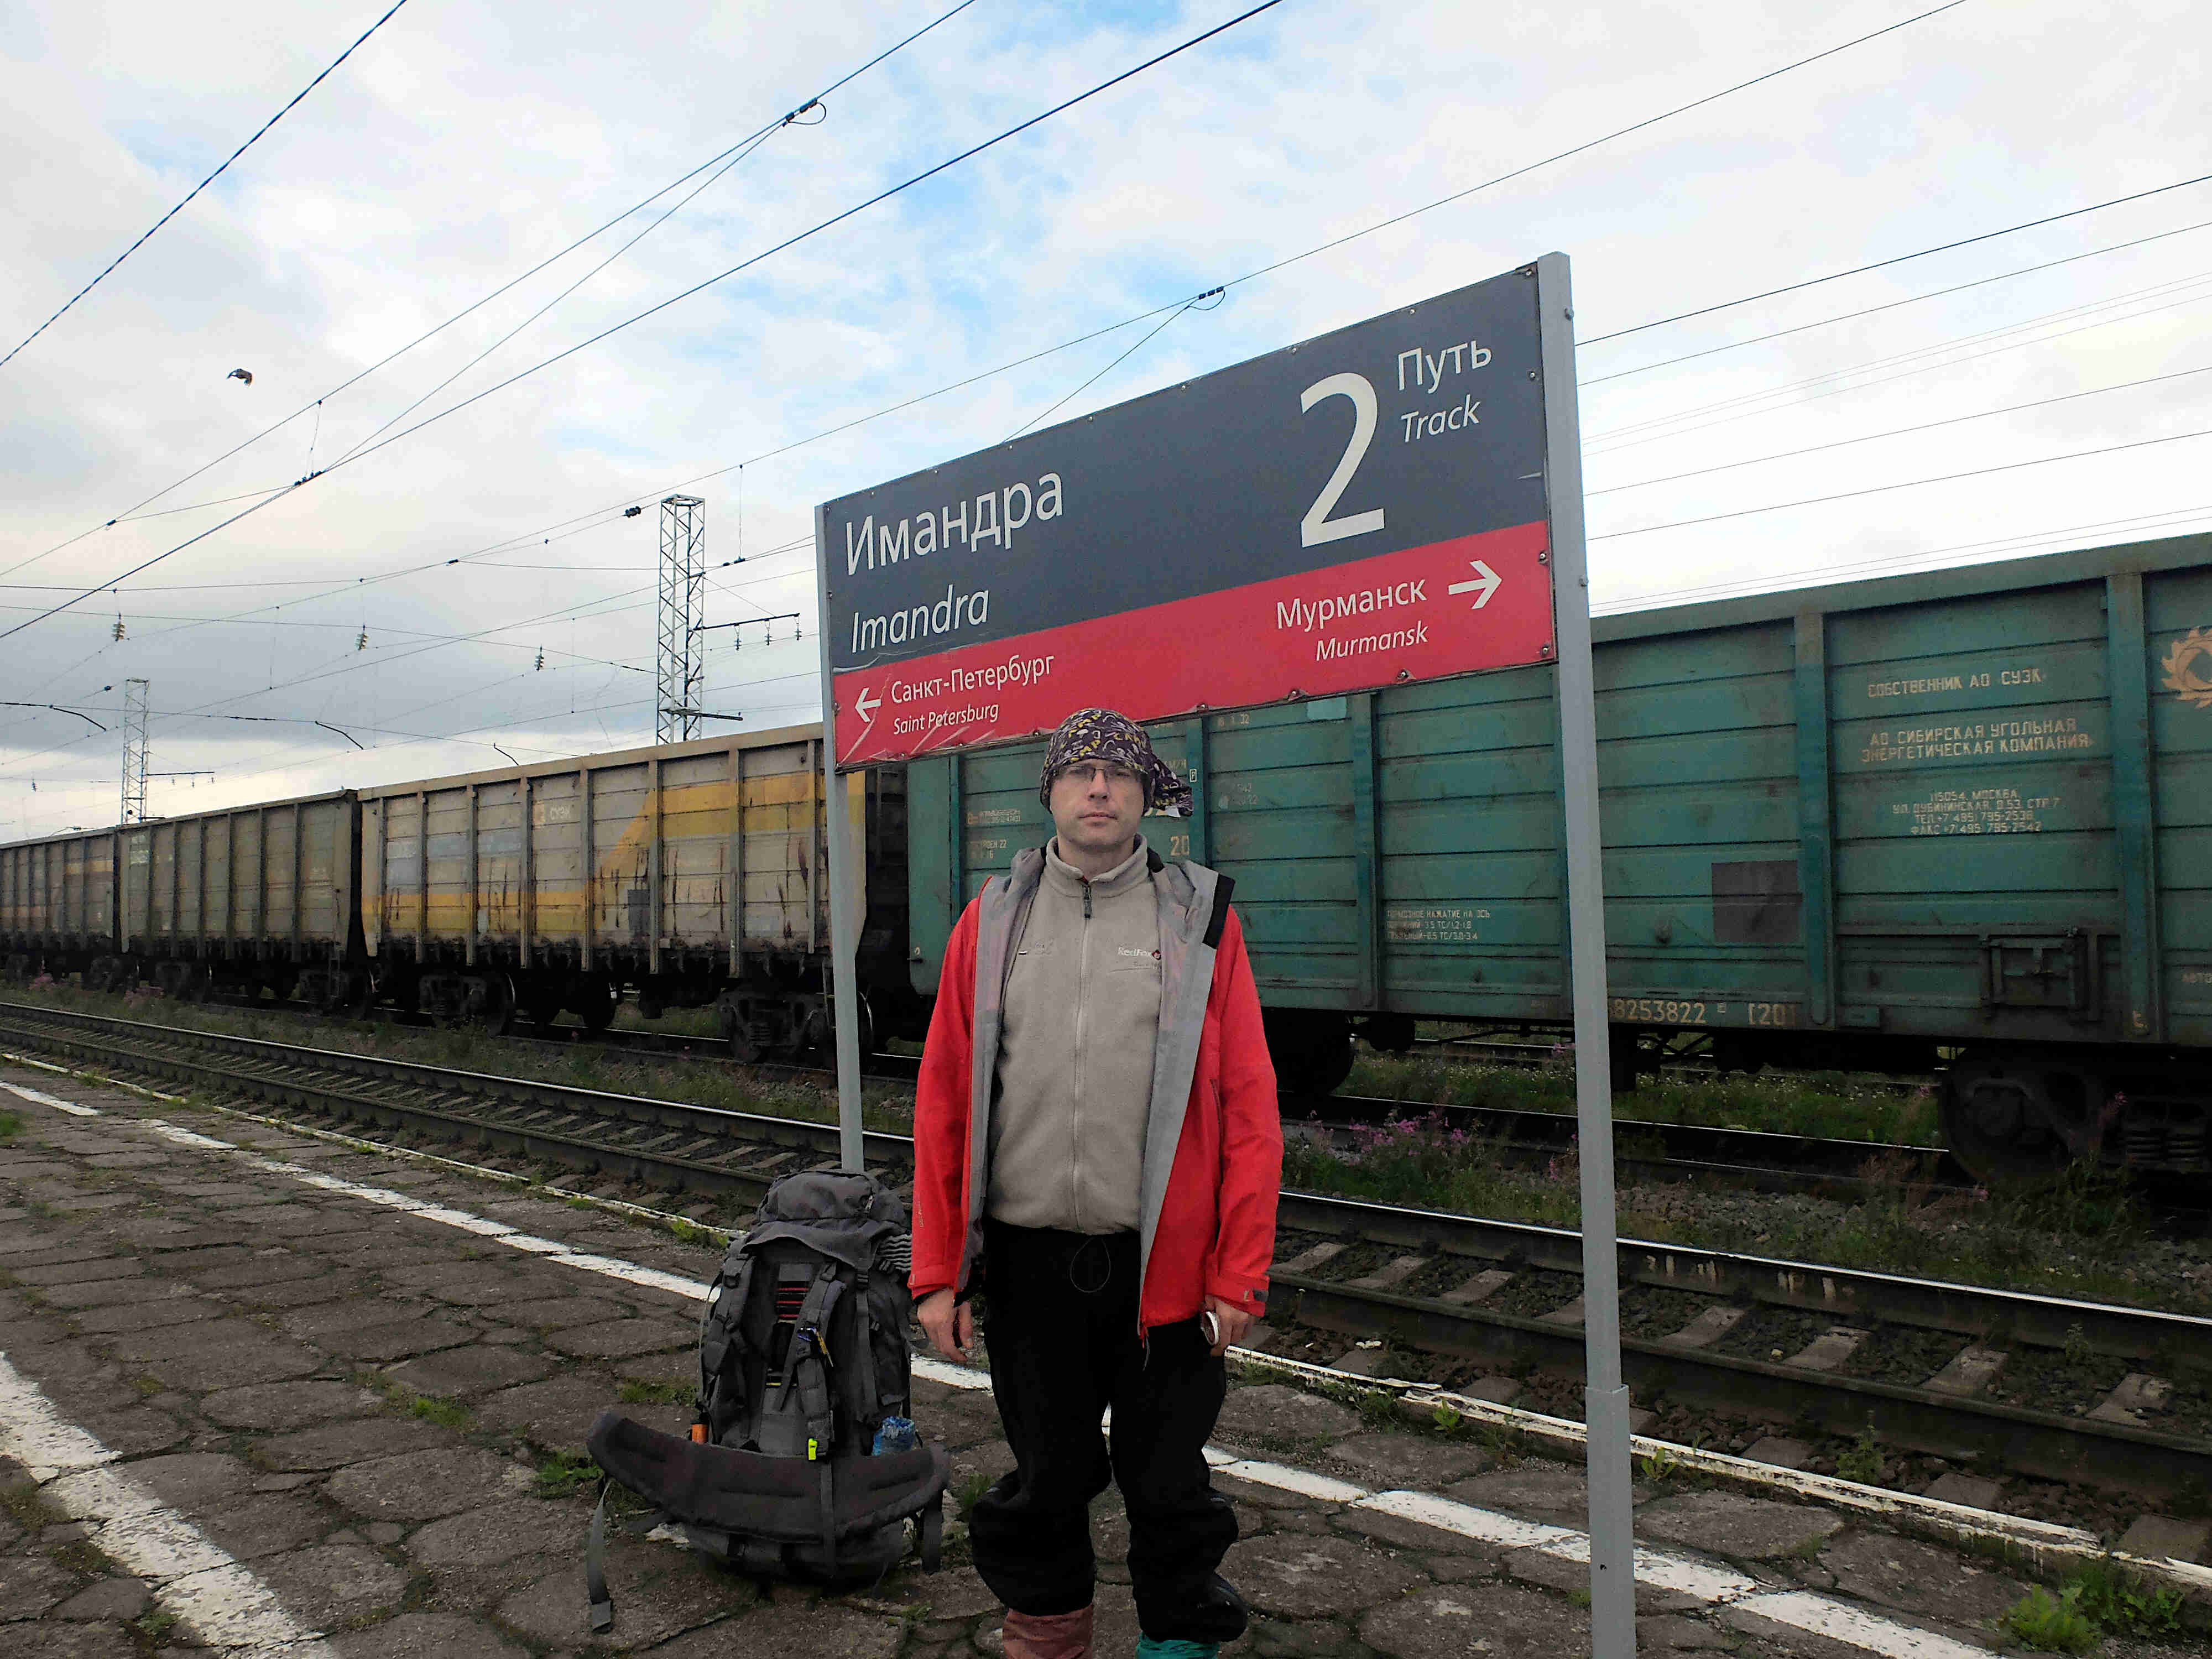
\includegraphics[width=14cm]{foto/Лица/mordas1_21.JPG}
    \caption{На старте}
    \label{fig1:1}
\end{figure}

\begin{figure}
    \centering
    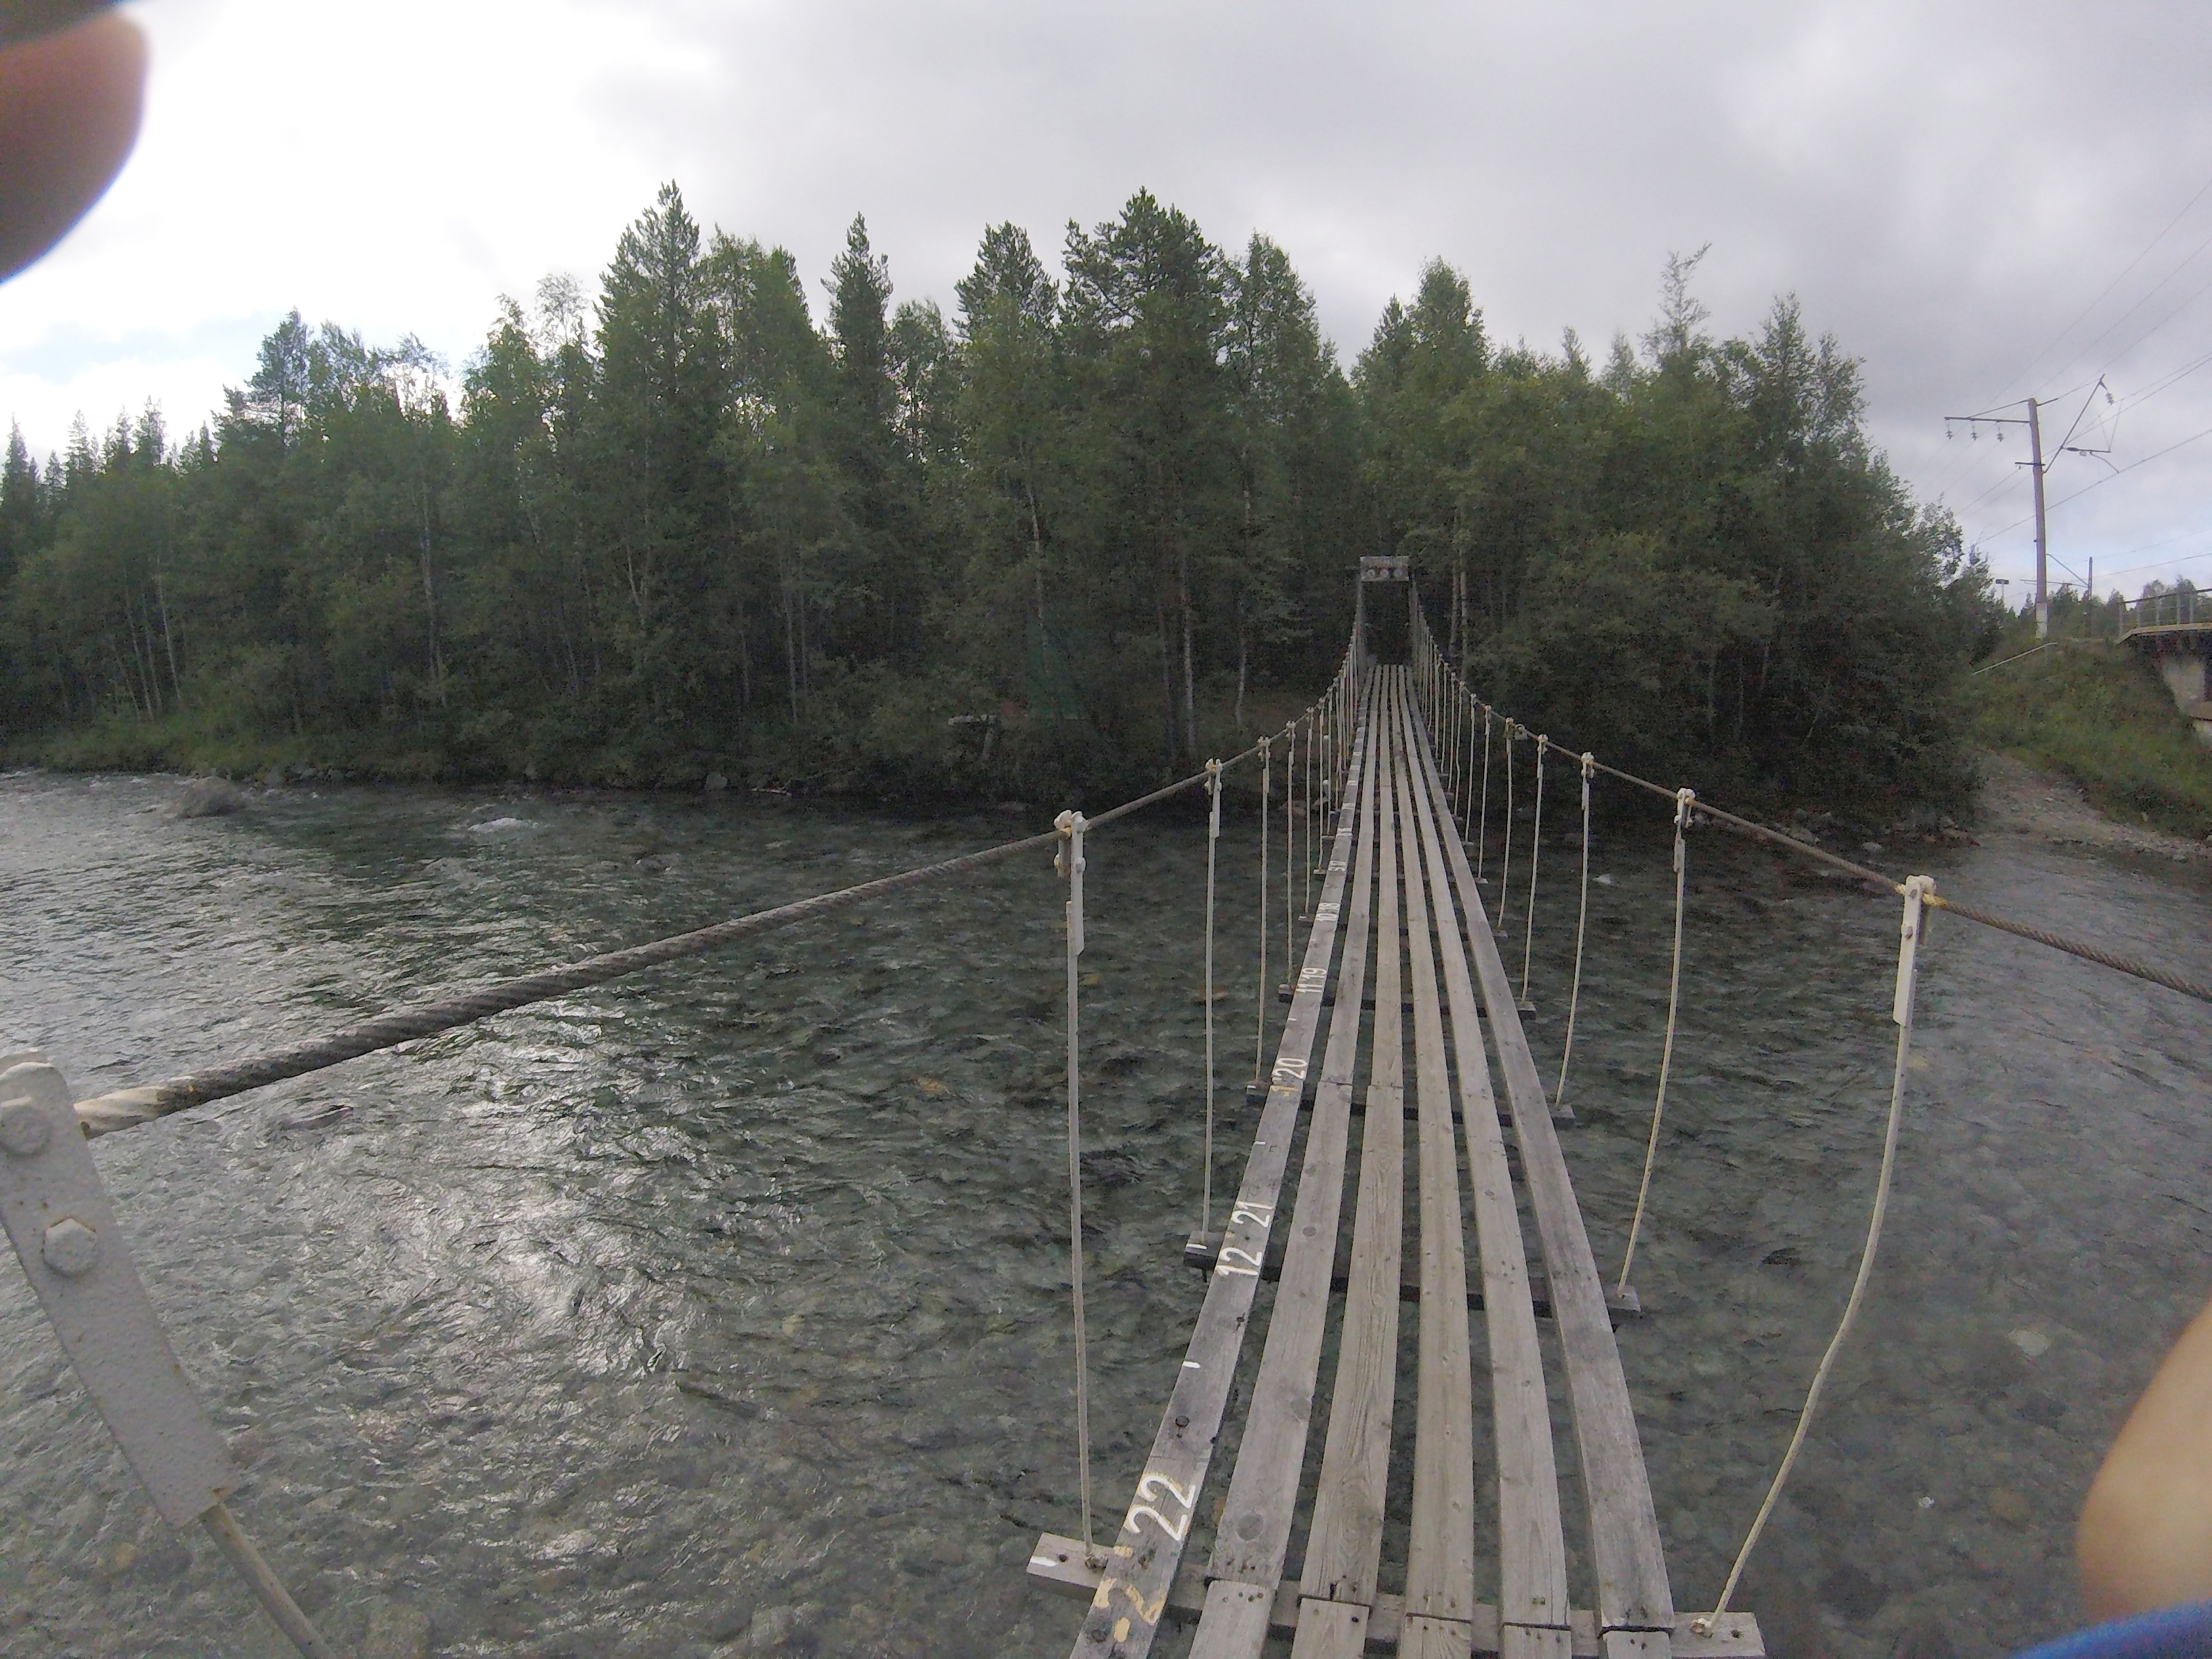
\includegraphics[width=14cm]{foto/05_08/01.Подвесной мост.png.jpg}
    \caption{Подвесной мост}
    \label{fig1:2}
\end{figure}

\begin{figure}
    \centering
    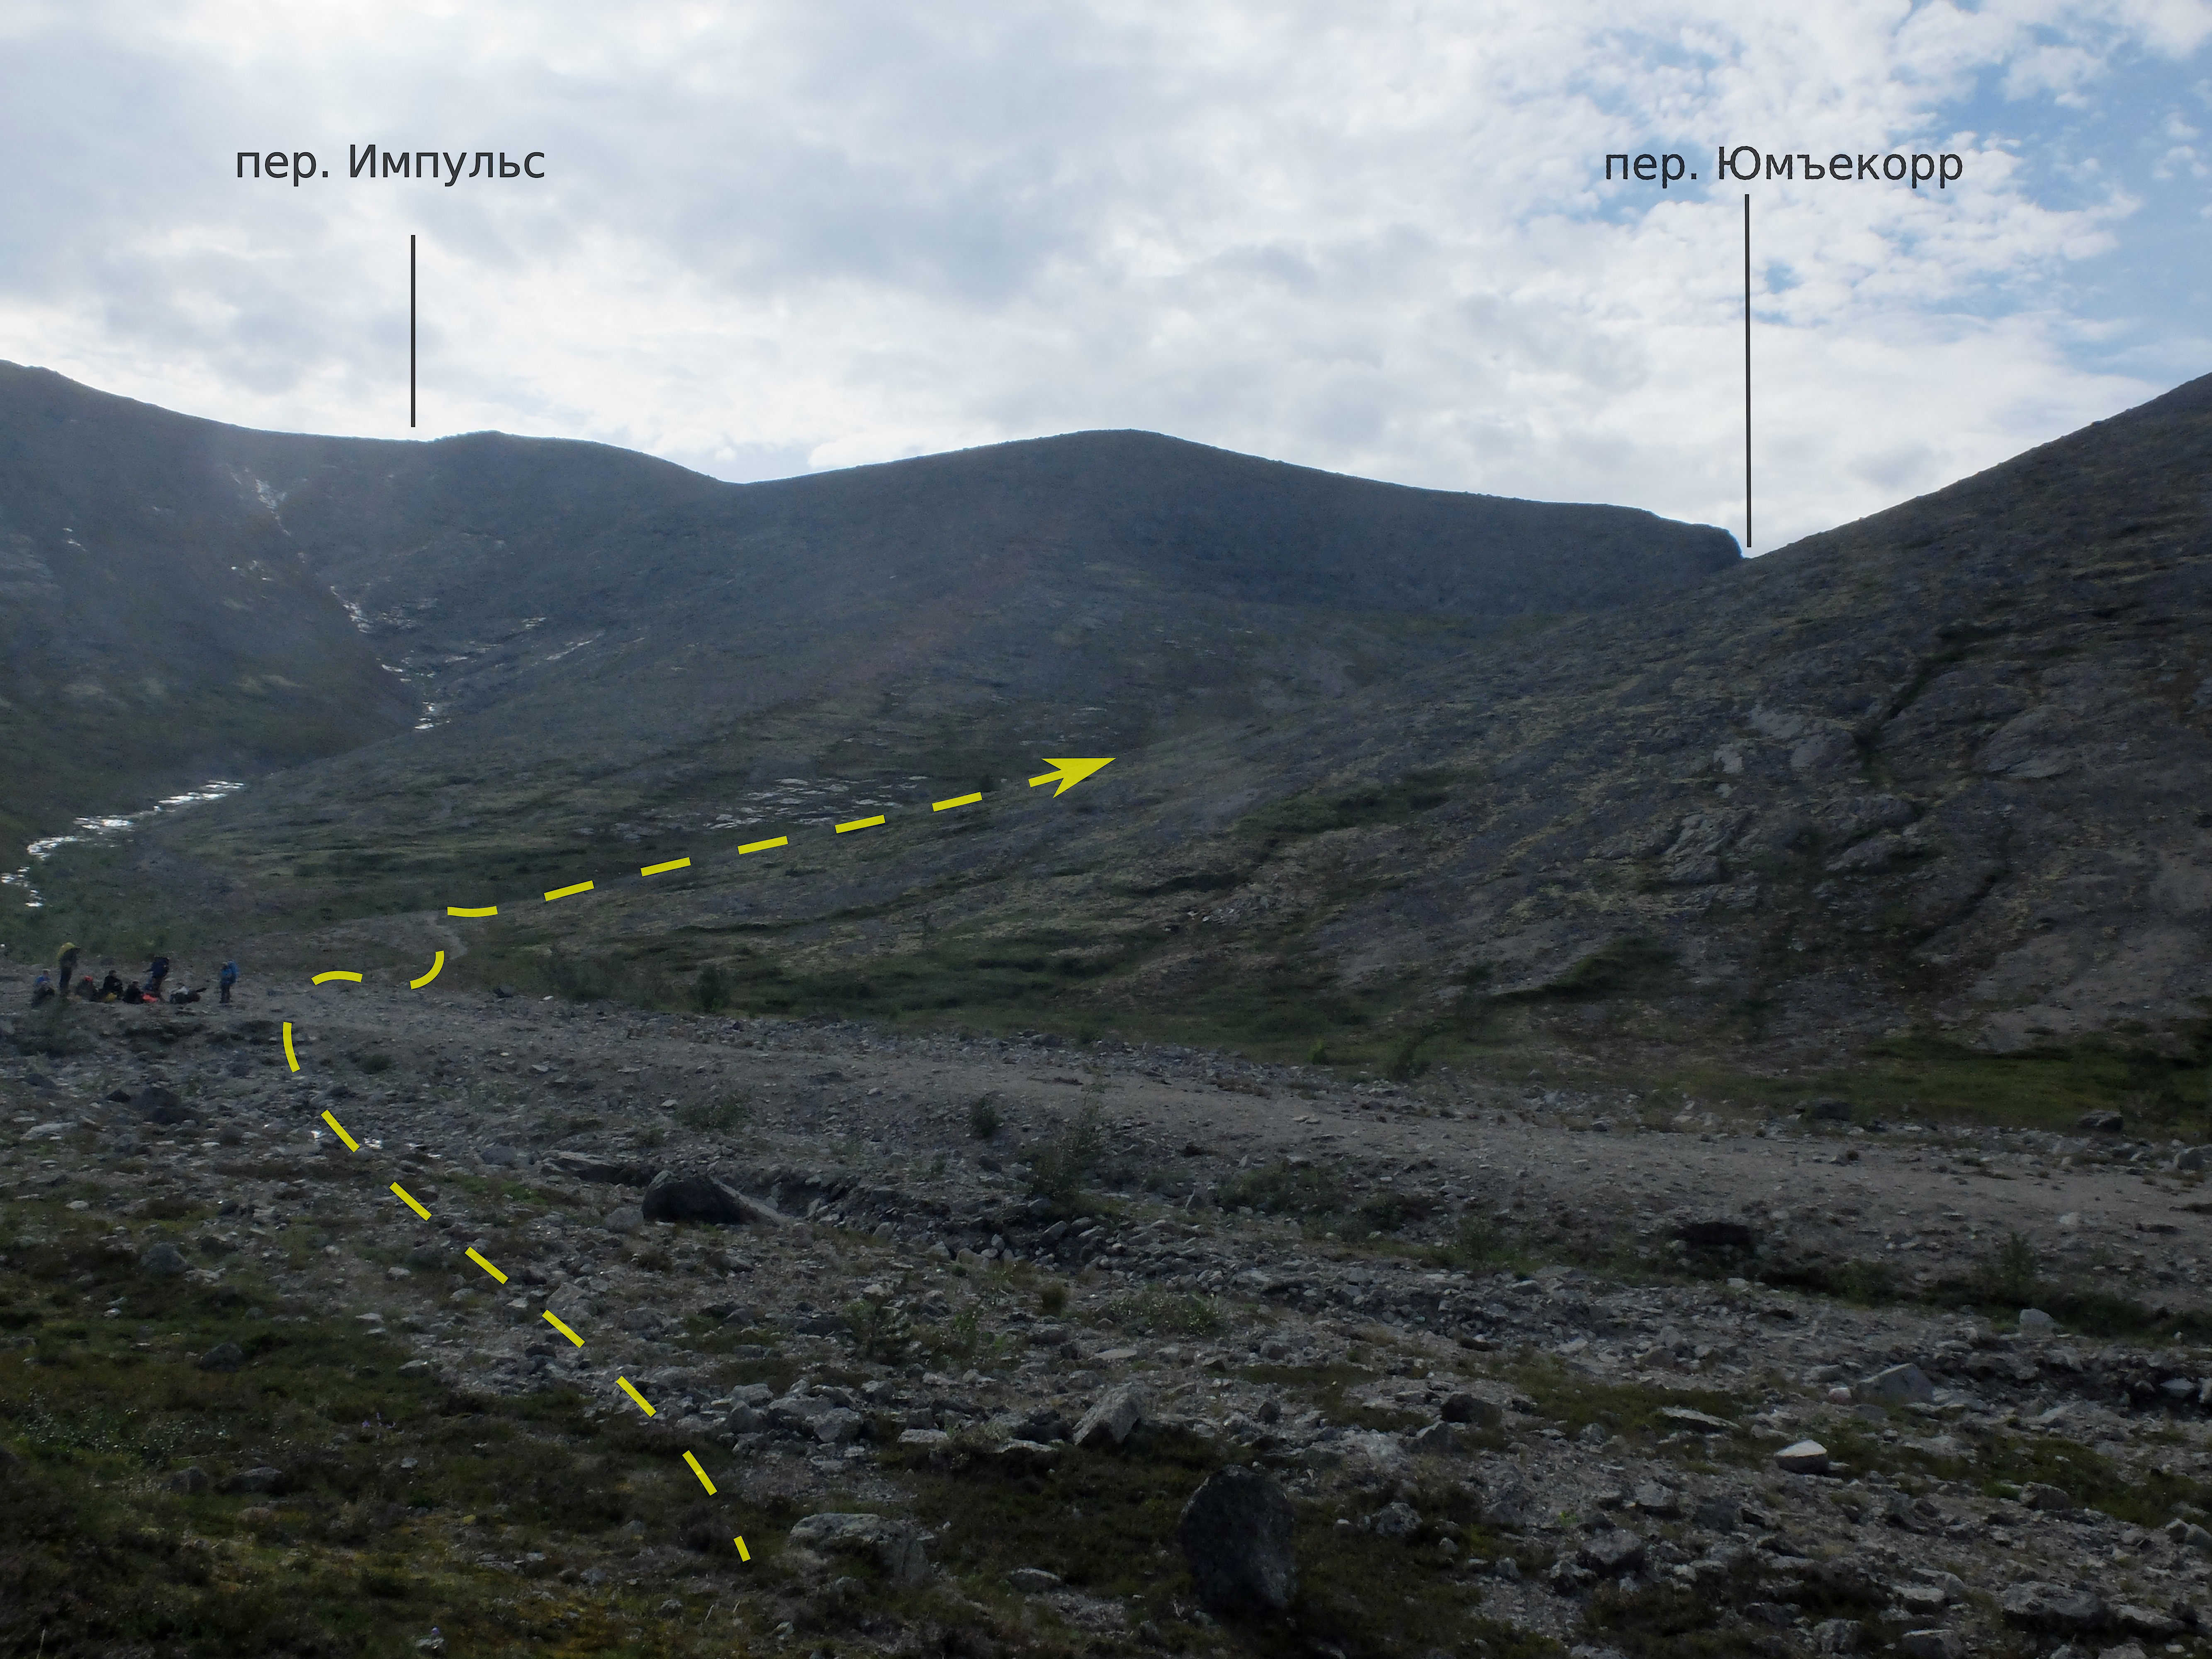
\includegraphics[width=14cm]{foto/05_08/02.Вид на подъем из долины.png.jpg}
    \caption{Вид на подъём на пер. Юмъекорр из долины руч. Меридионального}
    \label{fig1:3}
\end{figure}

\begin{figure}
    \centering
    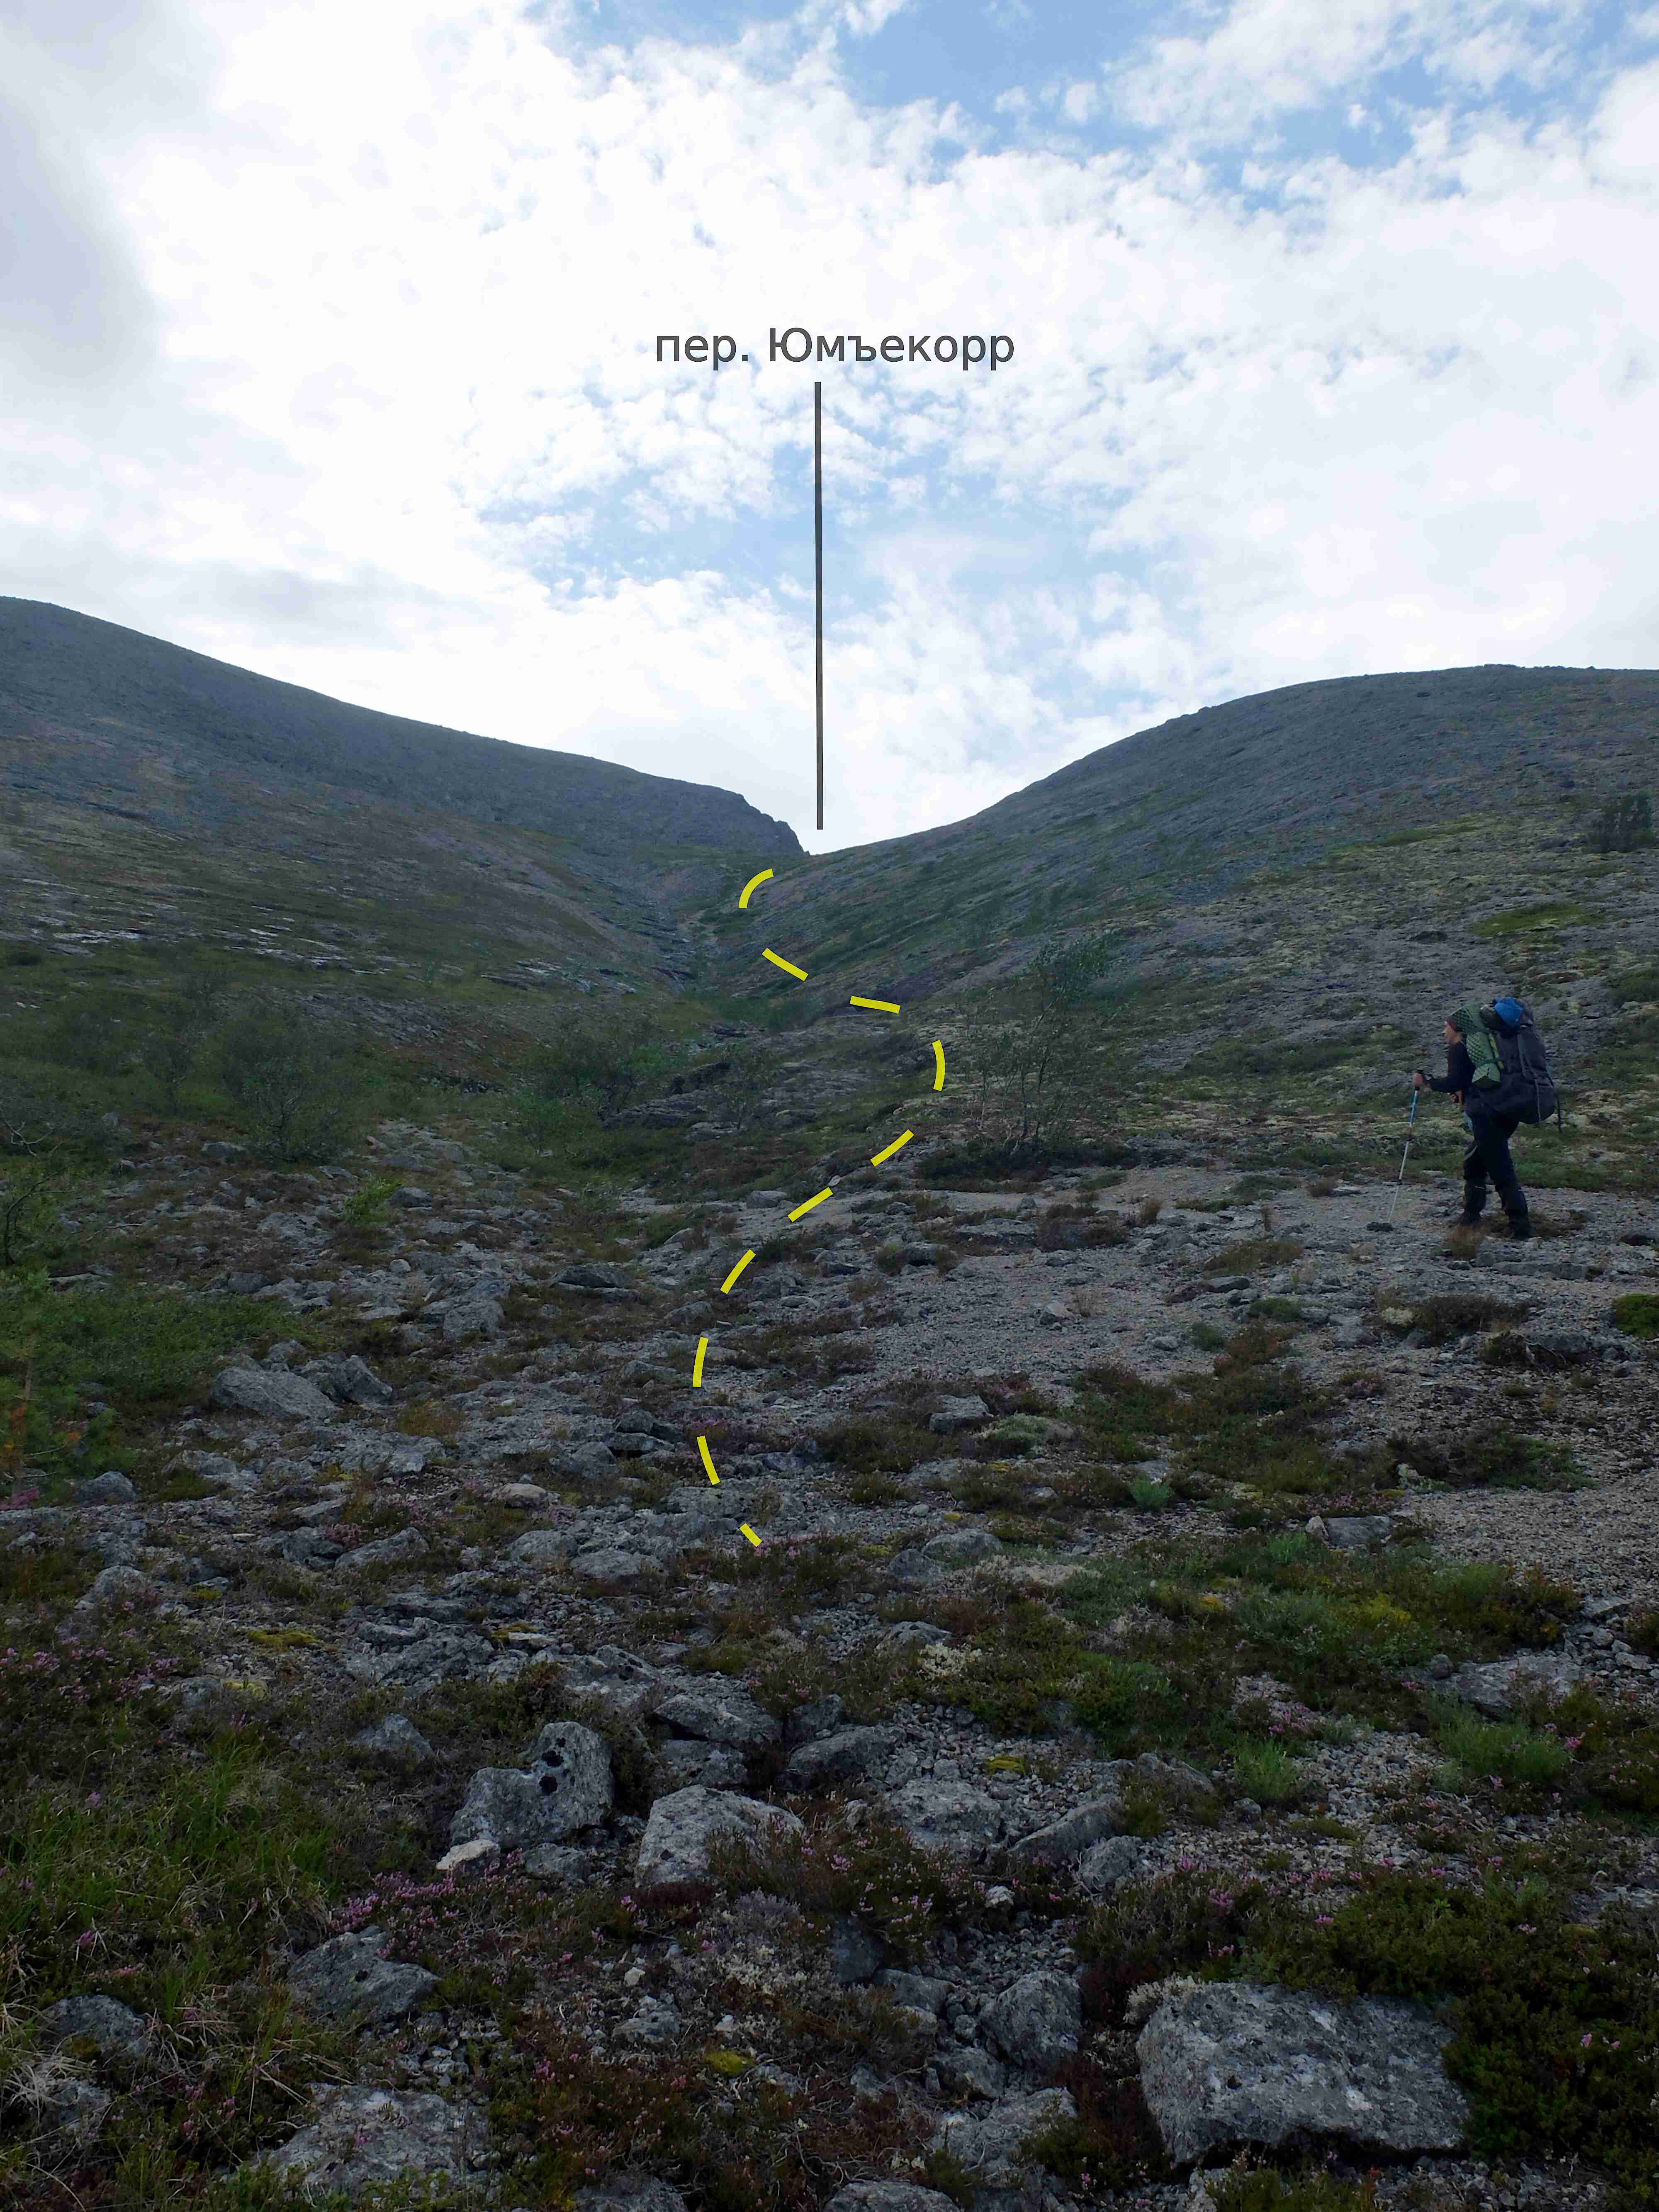
\includegraphics[width=16cm]{foto/05_08/03.Подъем на перевал.png.jpg}
    \caption{Подъём на пер. Юмъекорр из долины руч. Меридионального}
    \label{fig1:4}
\end{figure}

\begin{figure}
    \centering
    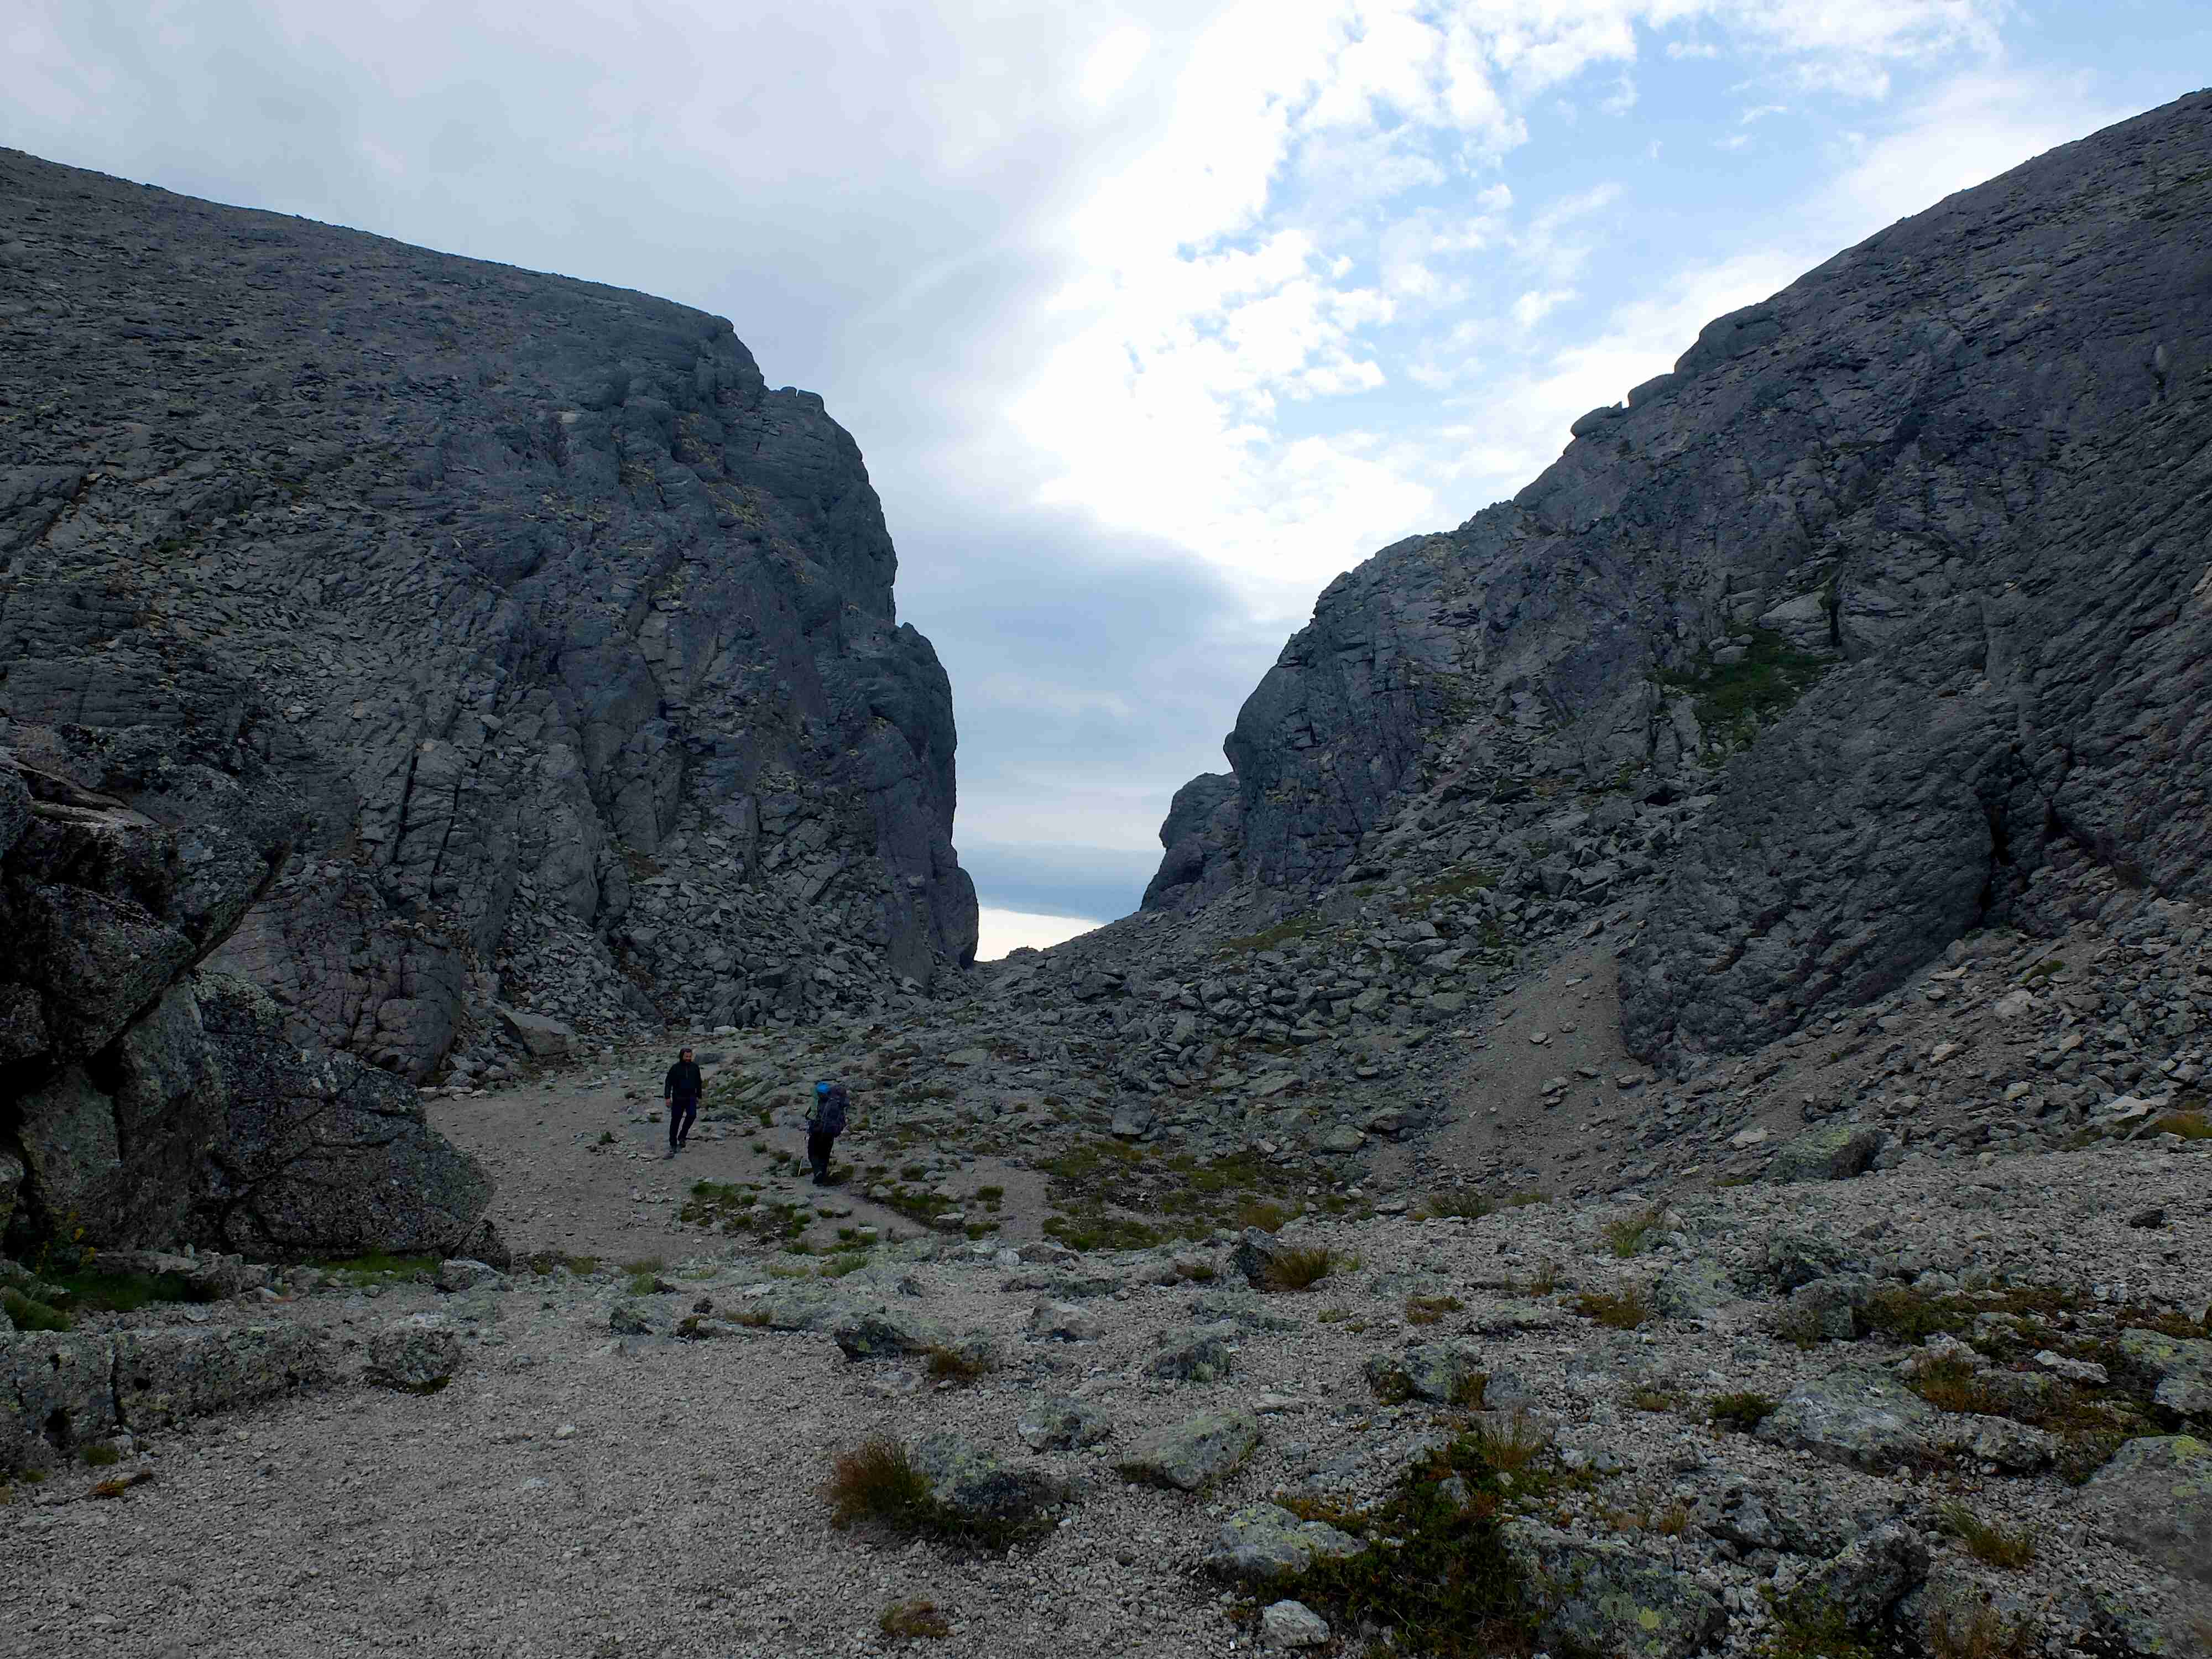
\includegraphics[width=14cm]{foto/05_08/04.Перевал с востока.png.jpg}
    \caption{Пер. Юмъекорр с востока}
    \label{fig1:5}
\end{figure}

\begin{figure}
    \centering
    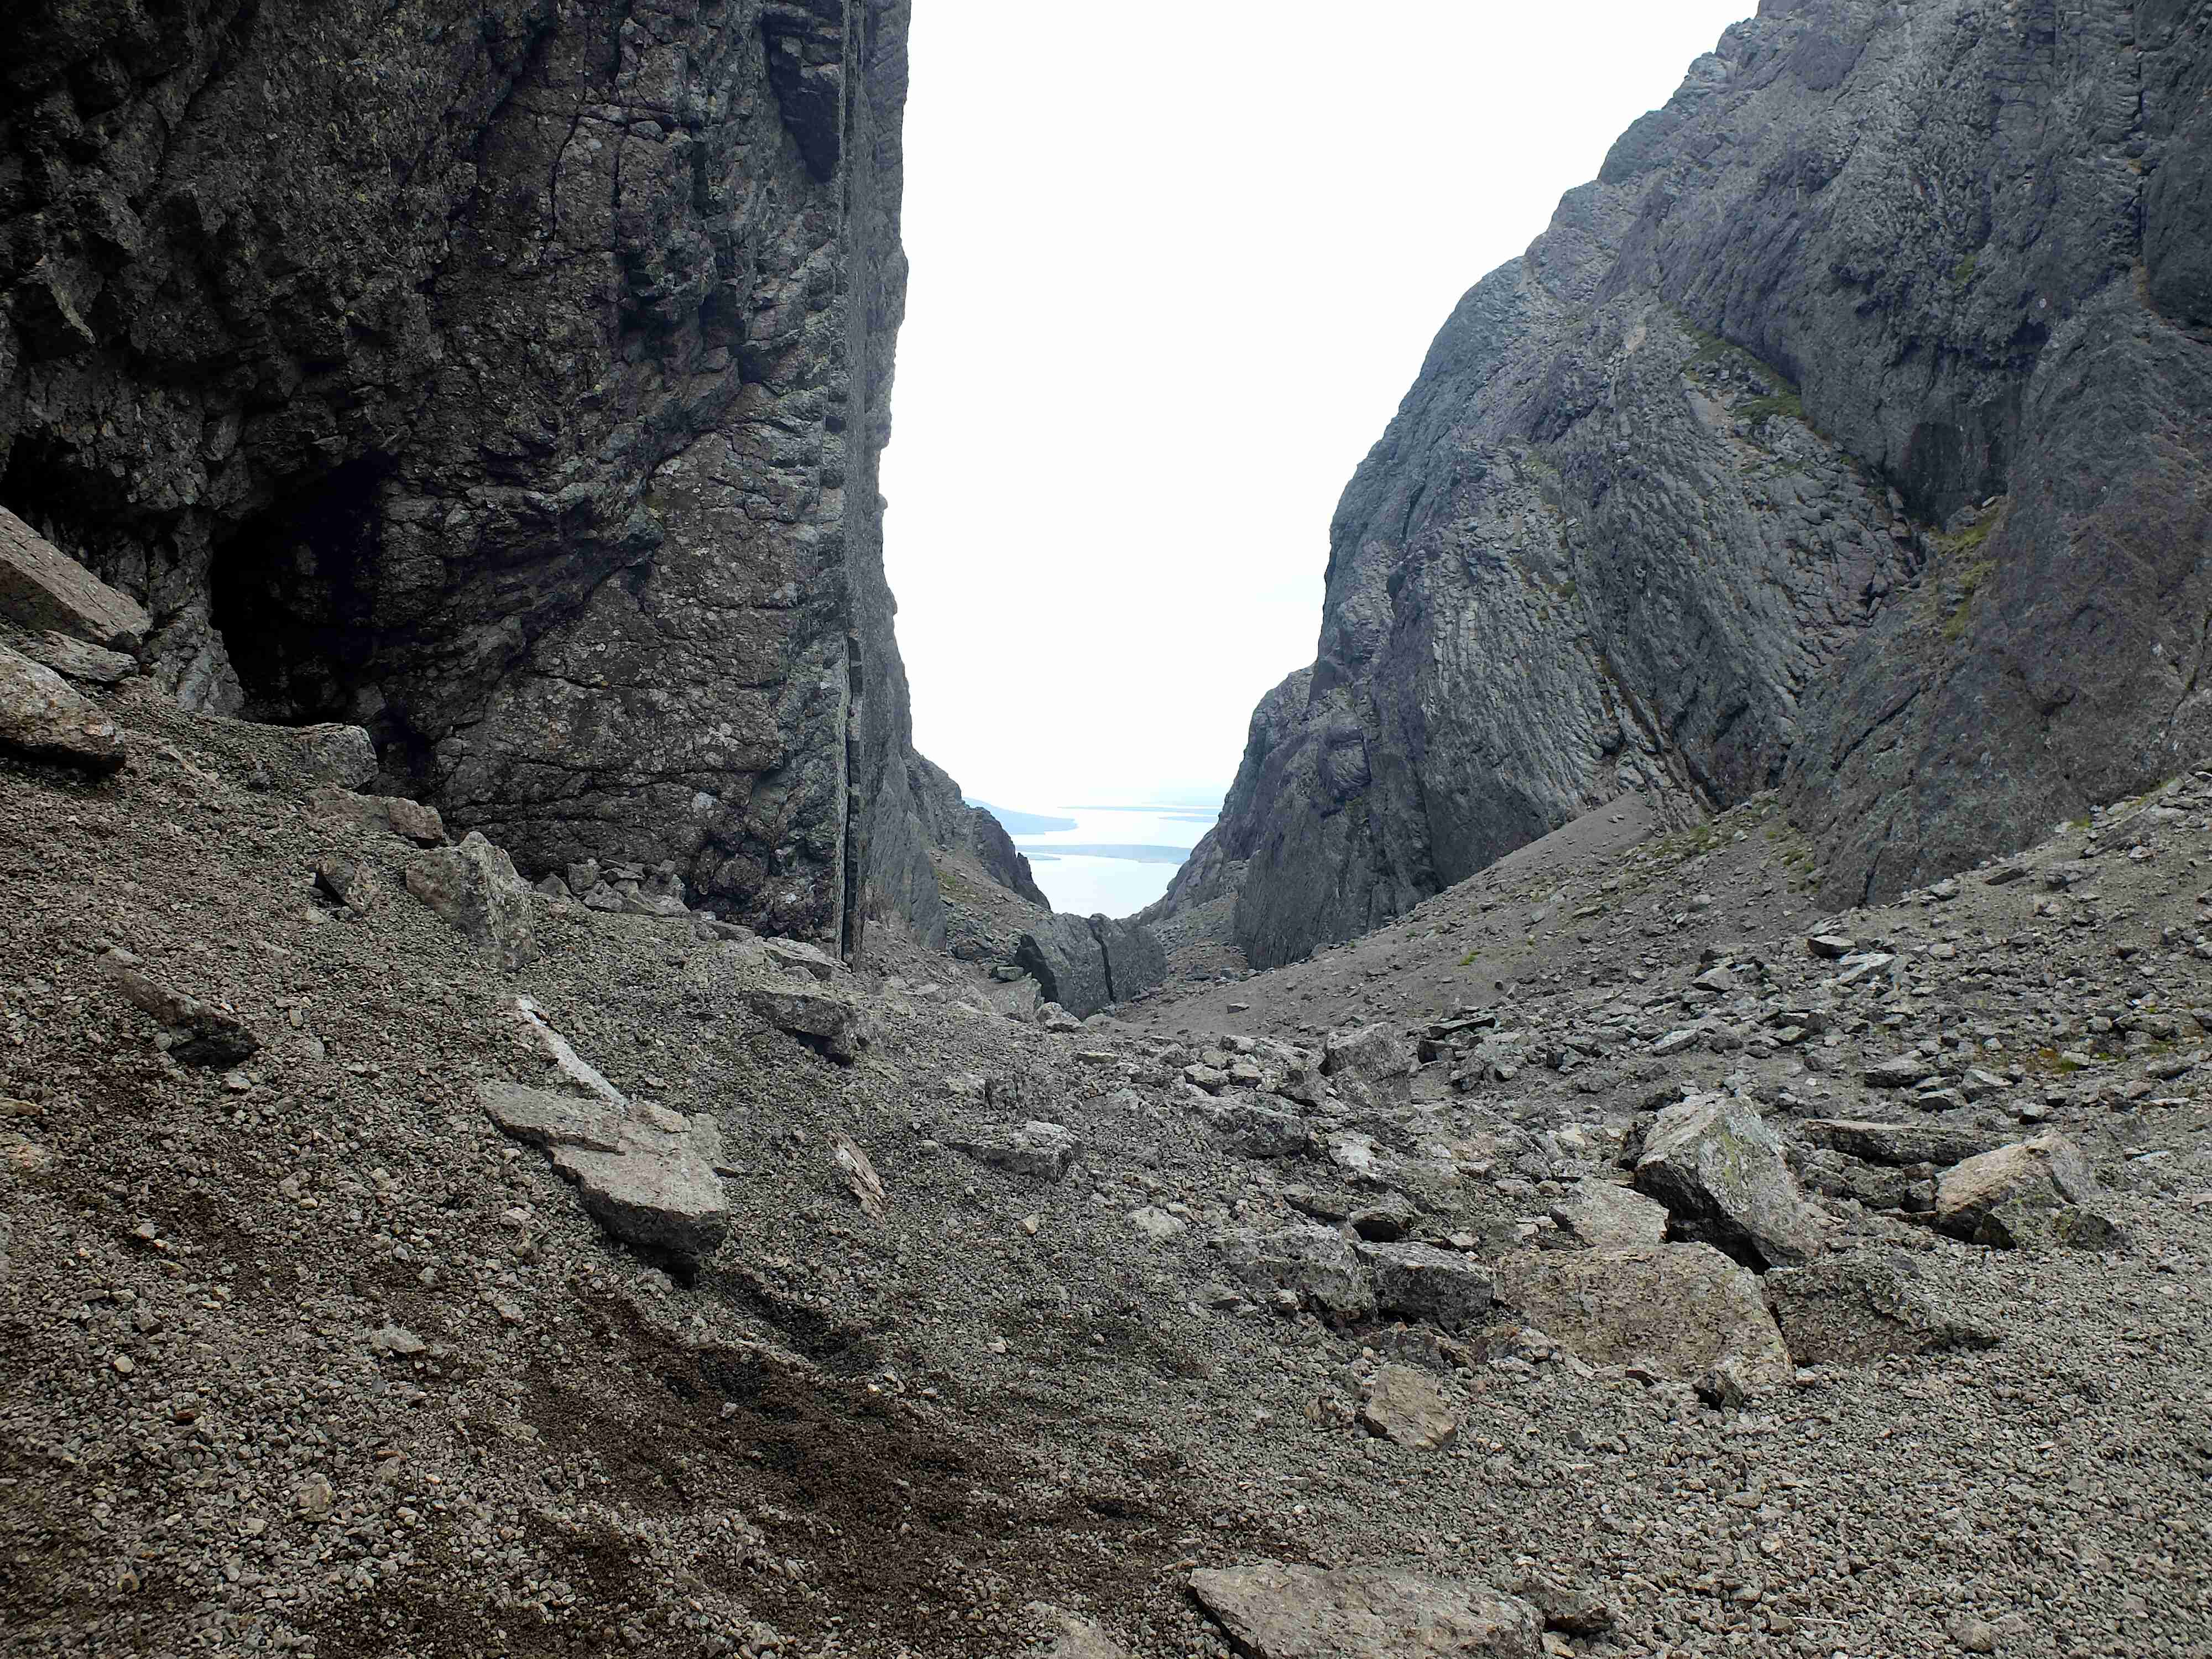
\includegraphics[width=14cm]{foto/05_08/05.Вид с перевала на запад.png.jpg}
    \caption{Вид с пер. Юмъекорр на запад}
    \label{fig1:6}
\end{figure}

\begin{figure}
    \centering
    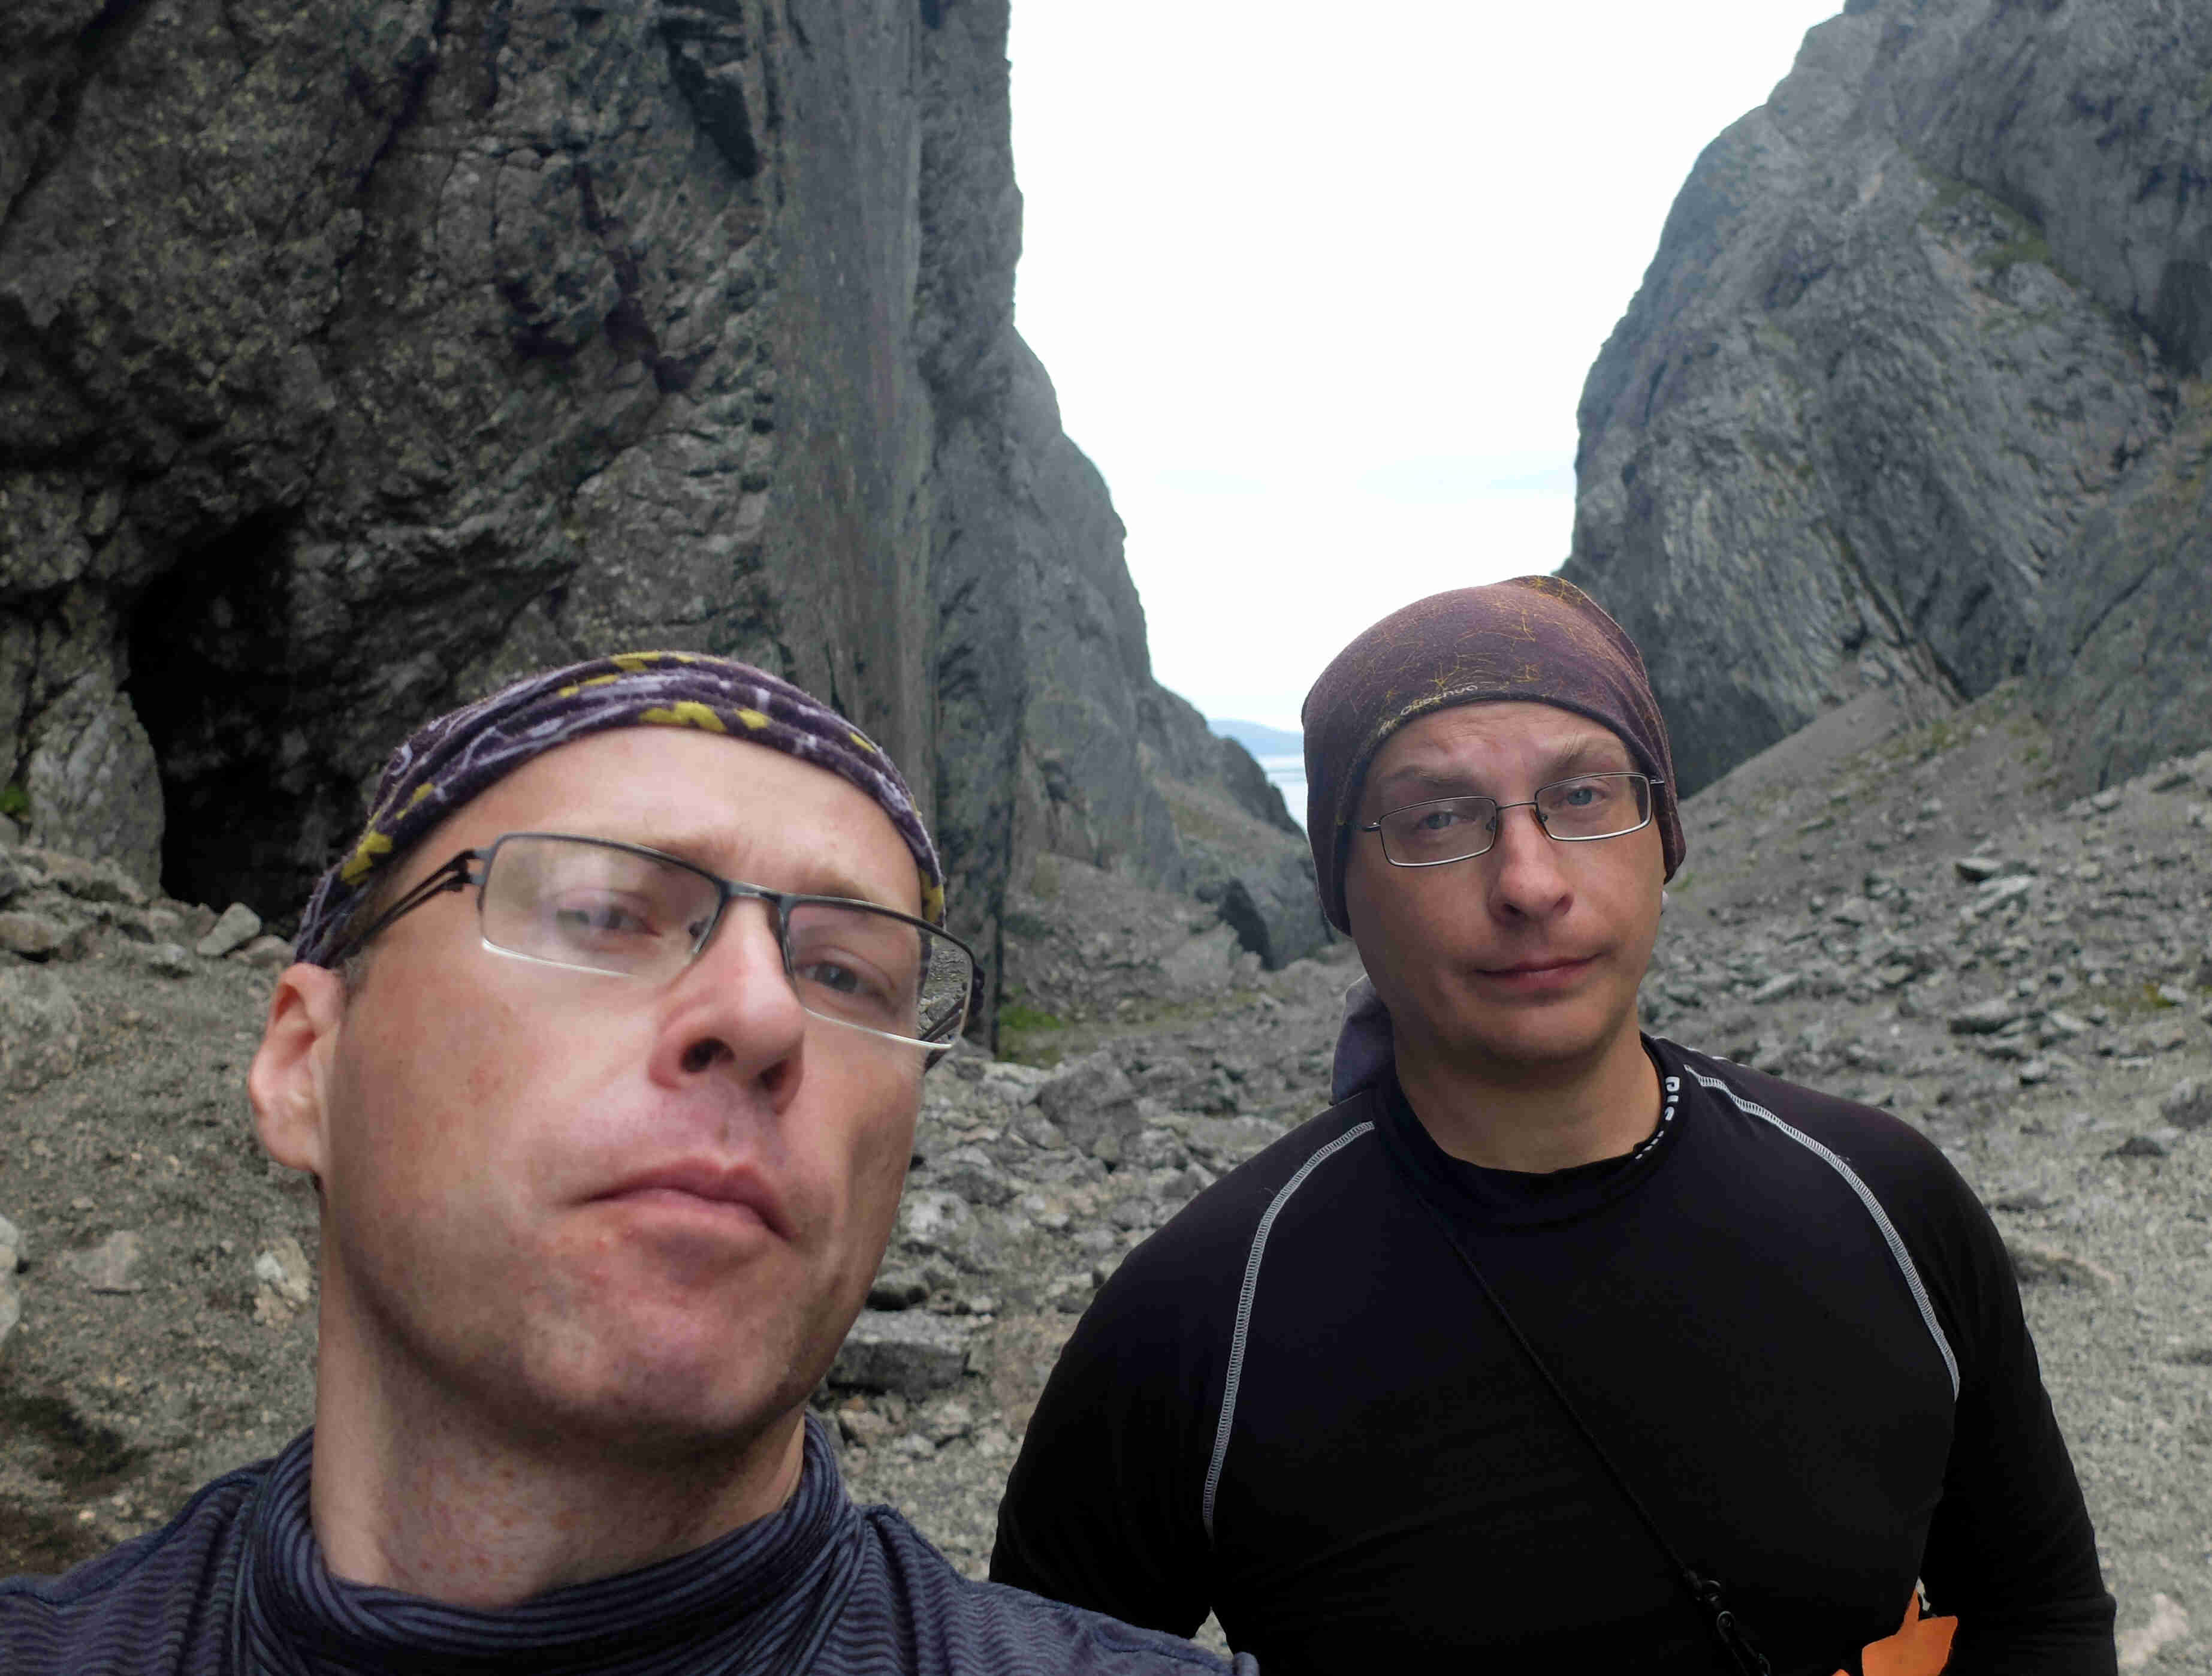
\includegraphics[width=14cm]{foto/Лица/mordas2.JPG}
    \caption{Фото группы на пер. Юмъекорр}
    \label{fig1:7}
\end{figure}

\begin{figure}
    \centering
    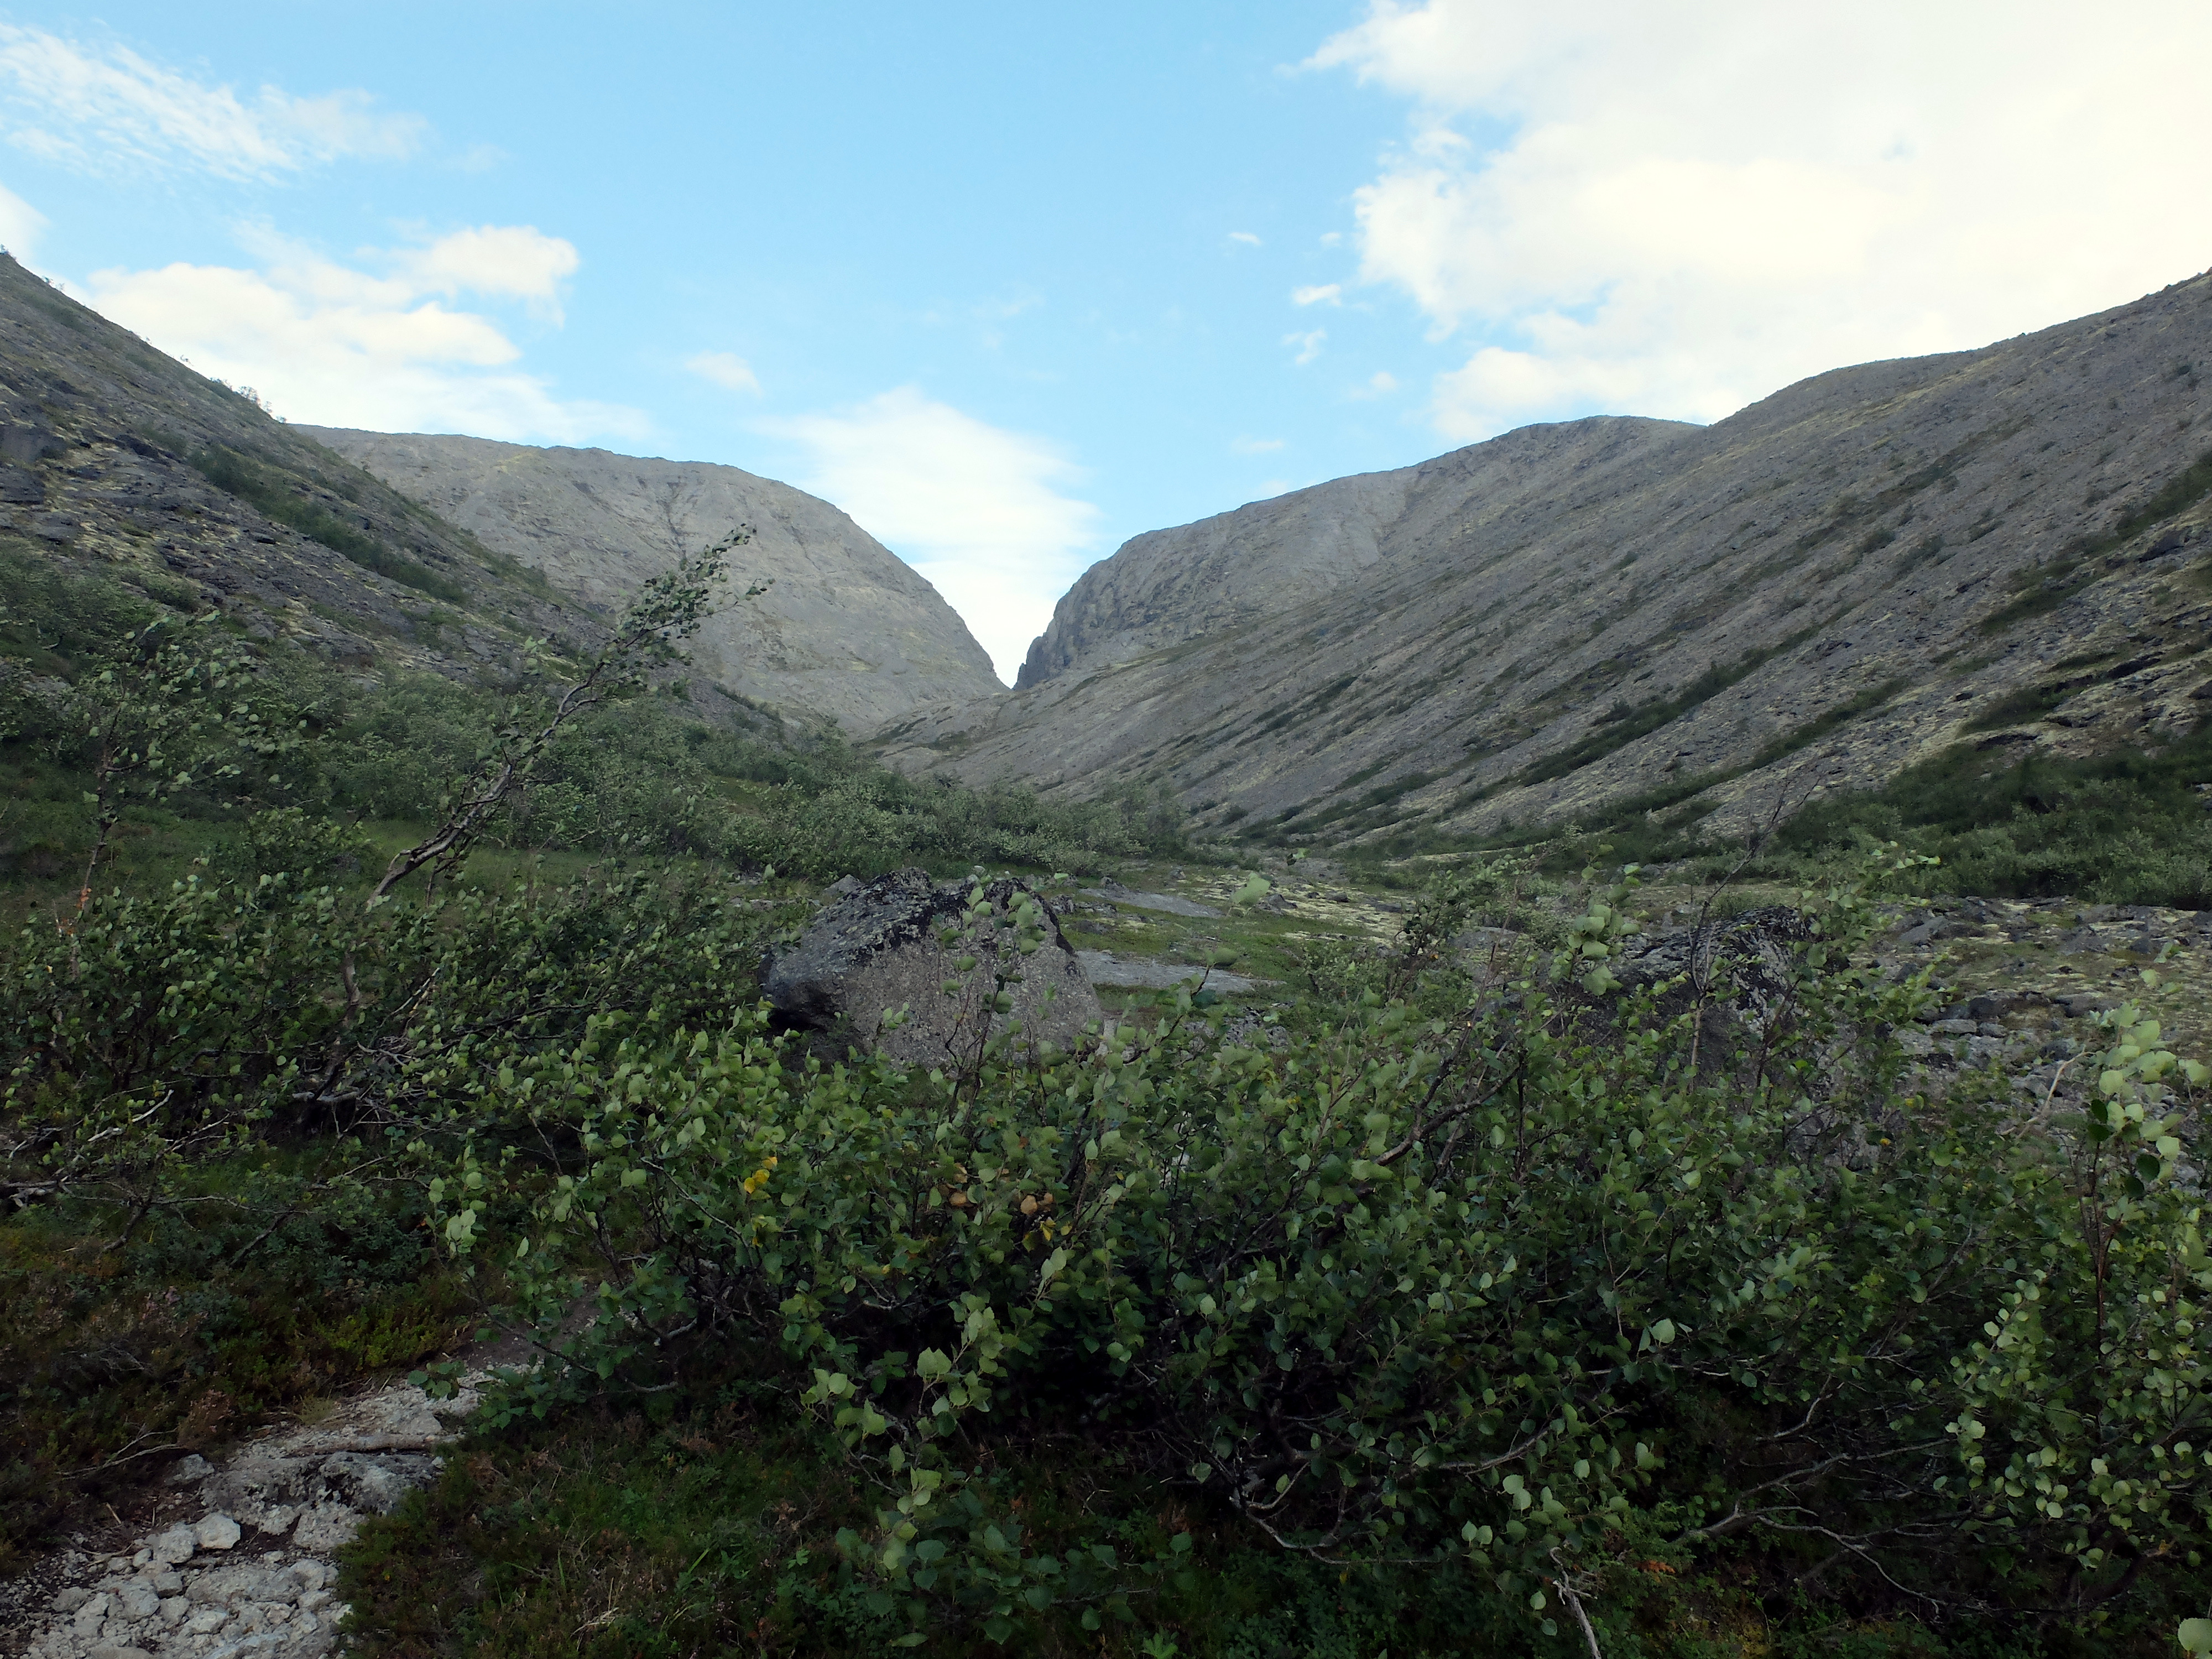
\includegraphics[width=14cm]{foto/05_08/06.Вид на перевал с запада.png.jpg}
    \caption{Вид на пер. Юмъекорр с запада}
    \label{fig1:8}
\end{figure}

\FloatBarrier

\subsection{День 2. 06.08.2022\\
Руч. Юмъекорруай -- ущ. Аку-Аку (рад.) -- ущ. Звездочка -- руч. Медвежий Лог}
\begin{tabular}{l p{12cm}}
\hline
Пройдено: & 14.1 км\\
Набор/сброс высоты: & 488/431 м\\
Время в пути: & 8:30\\
ЧХВ: & 5:39\\
Метеоусловия: & Пасмурно, временами дождь.\\
\hline
\end{tabular}

8:00 Подъём.
Ночью шёл дождь, с утра также дождь, +20$\tccentigrade$.

10:05 Собрали лагерь, выходим. Сначала идём смотреть ущелье Аку-Аку радиально.
Переходим на другую сторону руч. Юмъекорруай и спускаемся 180 метров до впадения ручья со стороны Аку-Аку.
У слияния большой лагерь туристов, часть бродит кругом и собирает ягоды. А мы идём в сторону Аку-Аку пока лагерь
с его обитателями не исчезает из вида, находим уступ над тропой и оставляем там рюкзаки в кустарнике.

10:21 Выходим к оз. Изумрудному. Путь до озера представляет из себя каменистую тропу, местами заболоченную,
приходится неоднократно пересекать ручьи. На южной оконечности озера большая и удобная поляна для стоянки,
на ней расположилось несколько групп туристов. Озеро можно обойти с востока: либо пройти по скальной полочке (рис. \ref{fig2:1}),
либо пройти по тропе над полочкой выше по осыпному склону. Решили пройти по полочке.
Полочка недлинная, но посреди расположен большой камень который пришлось облазить, один из участников пролез сбоку,
другой --- сверху (рис. \ref{fig2:2}).

Путь по ущелью после озера (севернее) представляет из себя каменистую тропу,
само ущелье часто перегорожено курумниками (рис. \ref{fig2:3}).
После озера прошли с километр, решили, что увидели достаточно, и повернули обратно 11:18.
В этот раз из интереса озеро обошли по тропе над скальной полкой.

12:20 Вернулись к рюкзакам. Небольшой перекус.

12:40 Идём дальше. Возвращаемся к руч. Юмъекорруай, переходим на другой берег, идём в сторону ущ. Звёздочка.
Почти сразу за ручьём ещё одна большая поляна со стоянками. В Звёздочку от неё ведёт тропа.
Само ущелье уютное, в отличие от мрачного Аку-Аку --- лесистое и очень тихое, глухое (рис. \ref{fig2:4});
только иногда кто-то из хищных птиц долго ухает нам вслед. Тропа большей частью идёт через лес, с холма на холм;
иногда попадаются средние камни, приходится переступать. Видно что тут ходят реже чем в Аку-Аку.

13:20 После ущелья тропа приводит нас к большой поляне со стоянкой на берегу руч.
Звёздочка, вытекающего из долины перевалов Нефелиновый и Юмъекорр боковой.
По берегу ручья идём на запад в сторону просеки ЛЭП и через 500 метров доходим до неё.
На карте вдоль ЛЭП идёт тропинка, по факту исчезающая. Поэтому проходим еще 300 метров до грунтовки к станции Хибины,
по которой мы начинали движение днем ранее. Дорога холмистая, постоянно вверх-вниз, много луж,
ездить по ней стоит скорее на \enquote{шишиге} или \enquote{буханке}.

По этой дороге доходим до руч. Нефелинового, где делаем привал на обед 14:03. Чтобы не досаждали комары,
останавливаемся на холме, где и растительность меньше, и комаров сдувает.

После обеда доходим до руч. Медвежий Лог 16:42. Нам вверх по ручью. По правому берегу идёт хорошая лесная тропа,
но через 2.5 километра лес заканчивается, а с ним и тропа. Переходим на другой берег. Тропы не находим;
идти вверх можно либо по самому ручью (хотя встречаются прижимы), либо поверху по склону. Метров через
300 в руч. Медвежий Лог впадает с севера приток из под пер. Почтальон, в месте слияния ручьев по берегам
есть удобные стоянки, там мы и останавливаемся на ночлег 18:39.
Пока готовили ужин шёл дождь, потом перестал, даже выглянуло закатное солнце.

Других людей на стоянке не было, связь также отсутствовала. И вообще было ощущение дикого места,
нет-нет --- да глянешь кругом, нет ли медведя. Зато кругом склоны с нетронутой голубикой, после ужина прошлись по ним.

21:30 отбой, пошёл дождь.

\begin{figure}
    \centering
    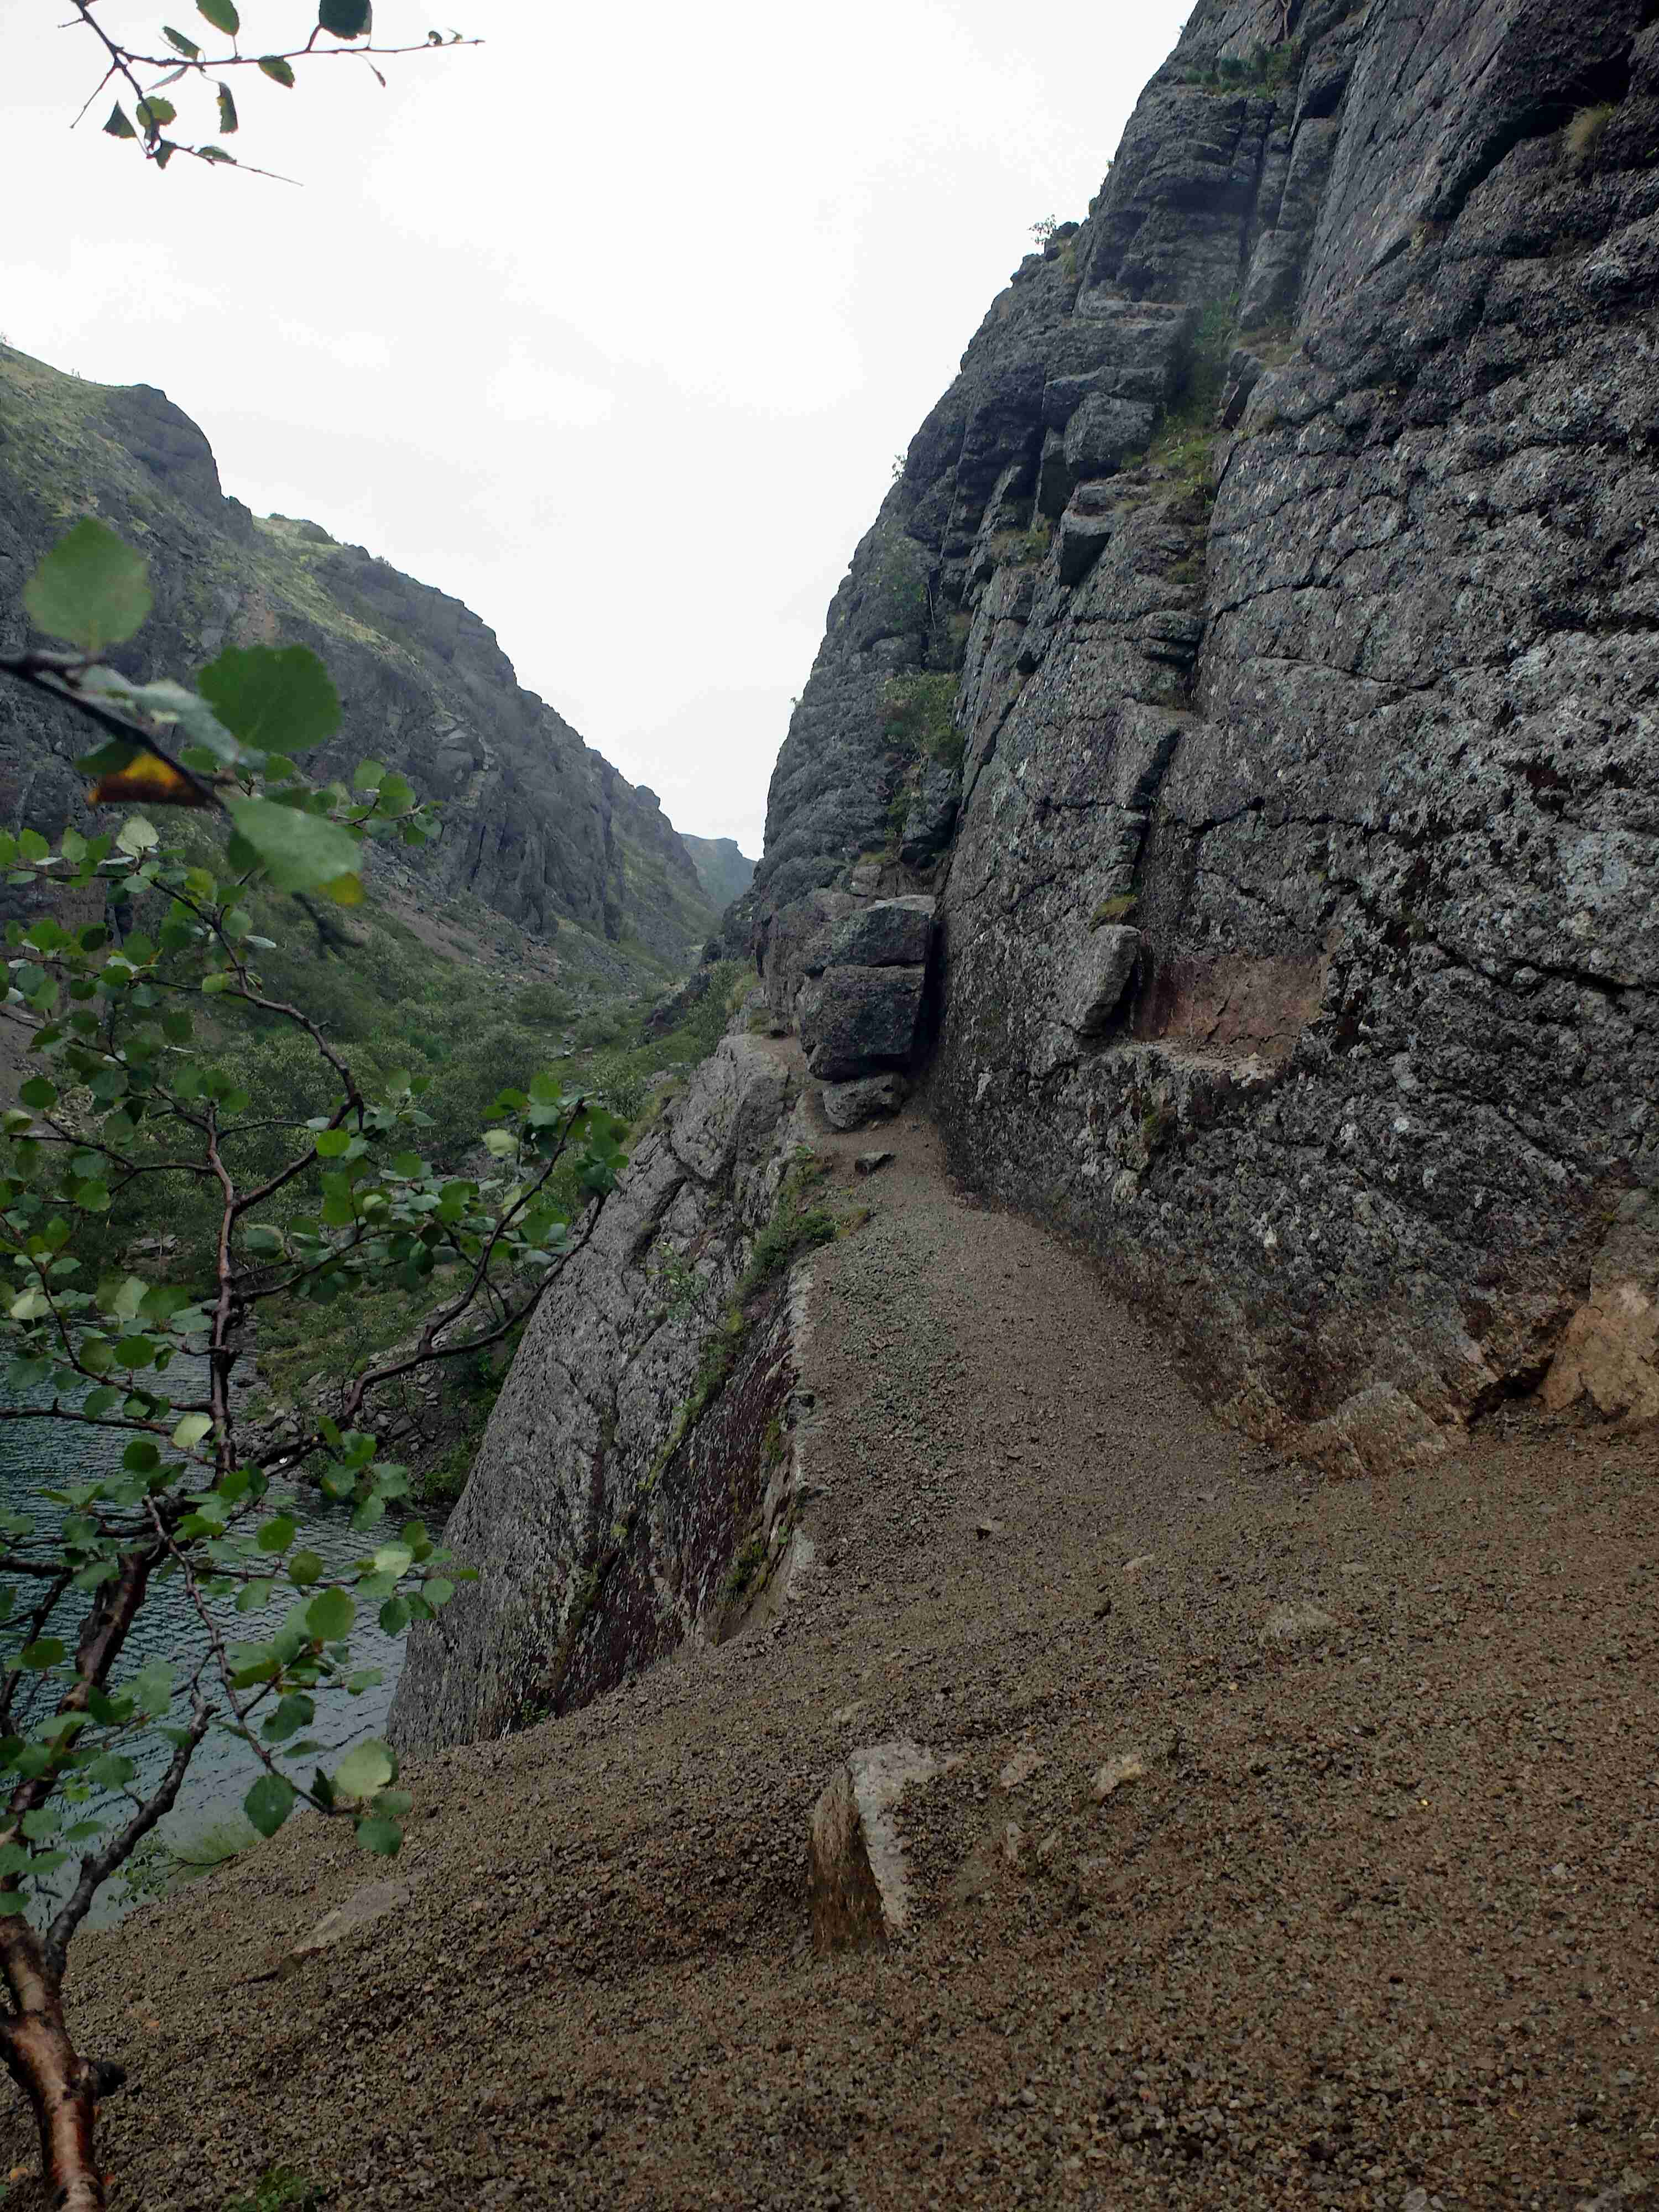
\includegraphics[width=14cm]{foto/06_08/01.Озеро и полочка.png.jpg}
    \caption{Скальная полка над оз. Изумрудным}
    \label{fig2:1}
\end{figure}

\begin{figure}
    \centering
    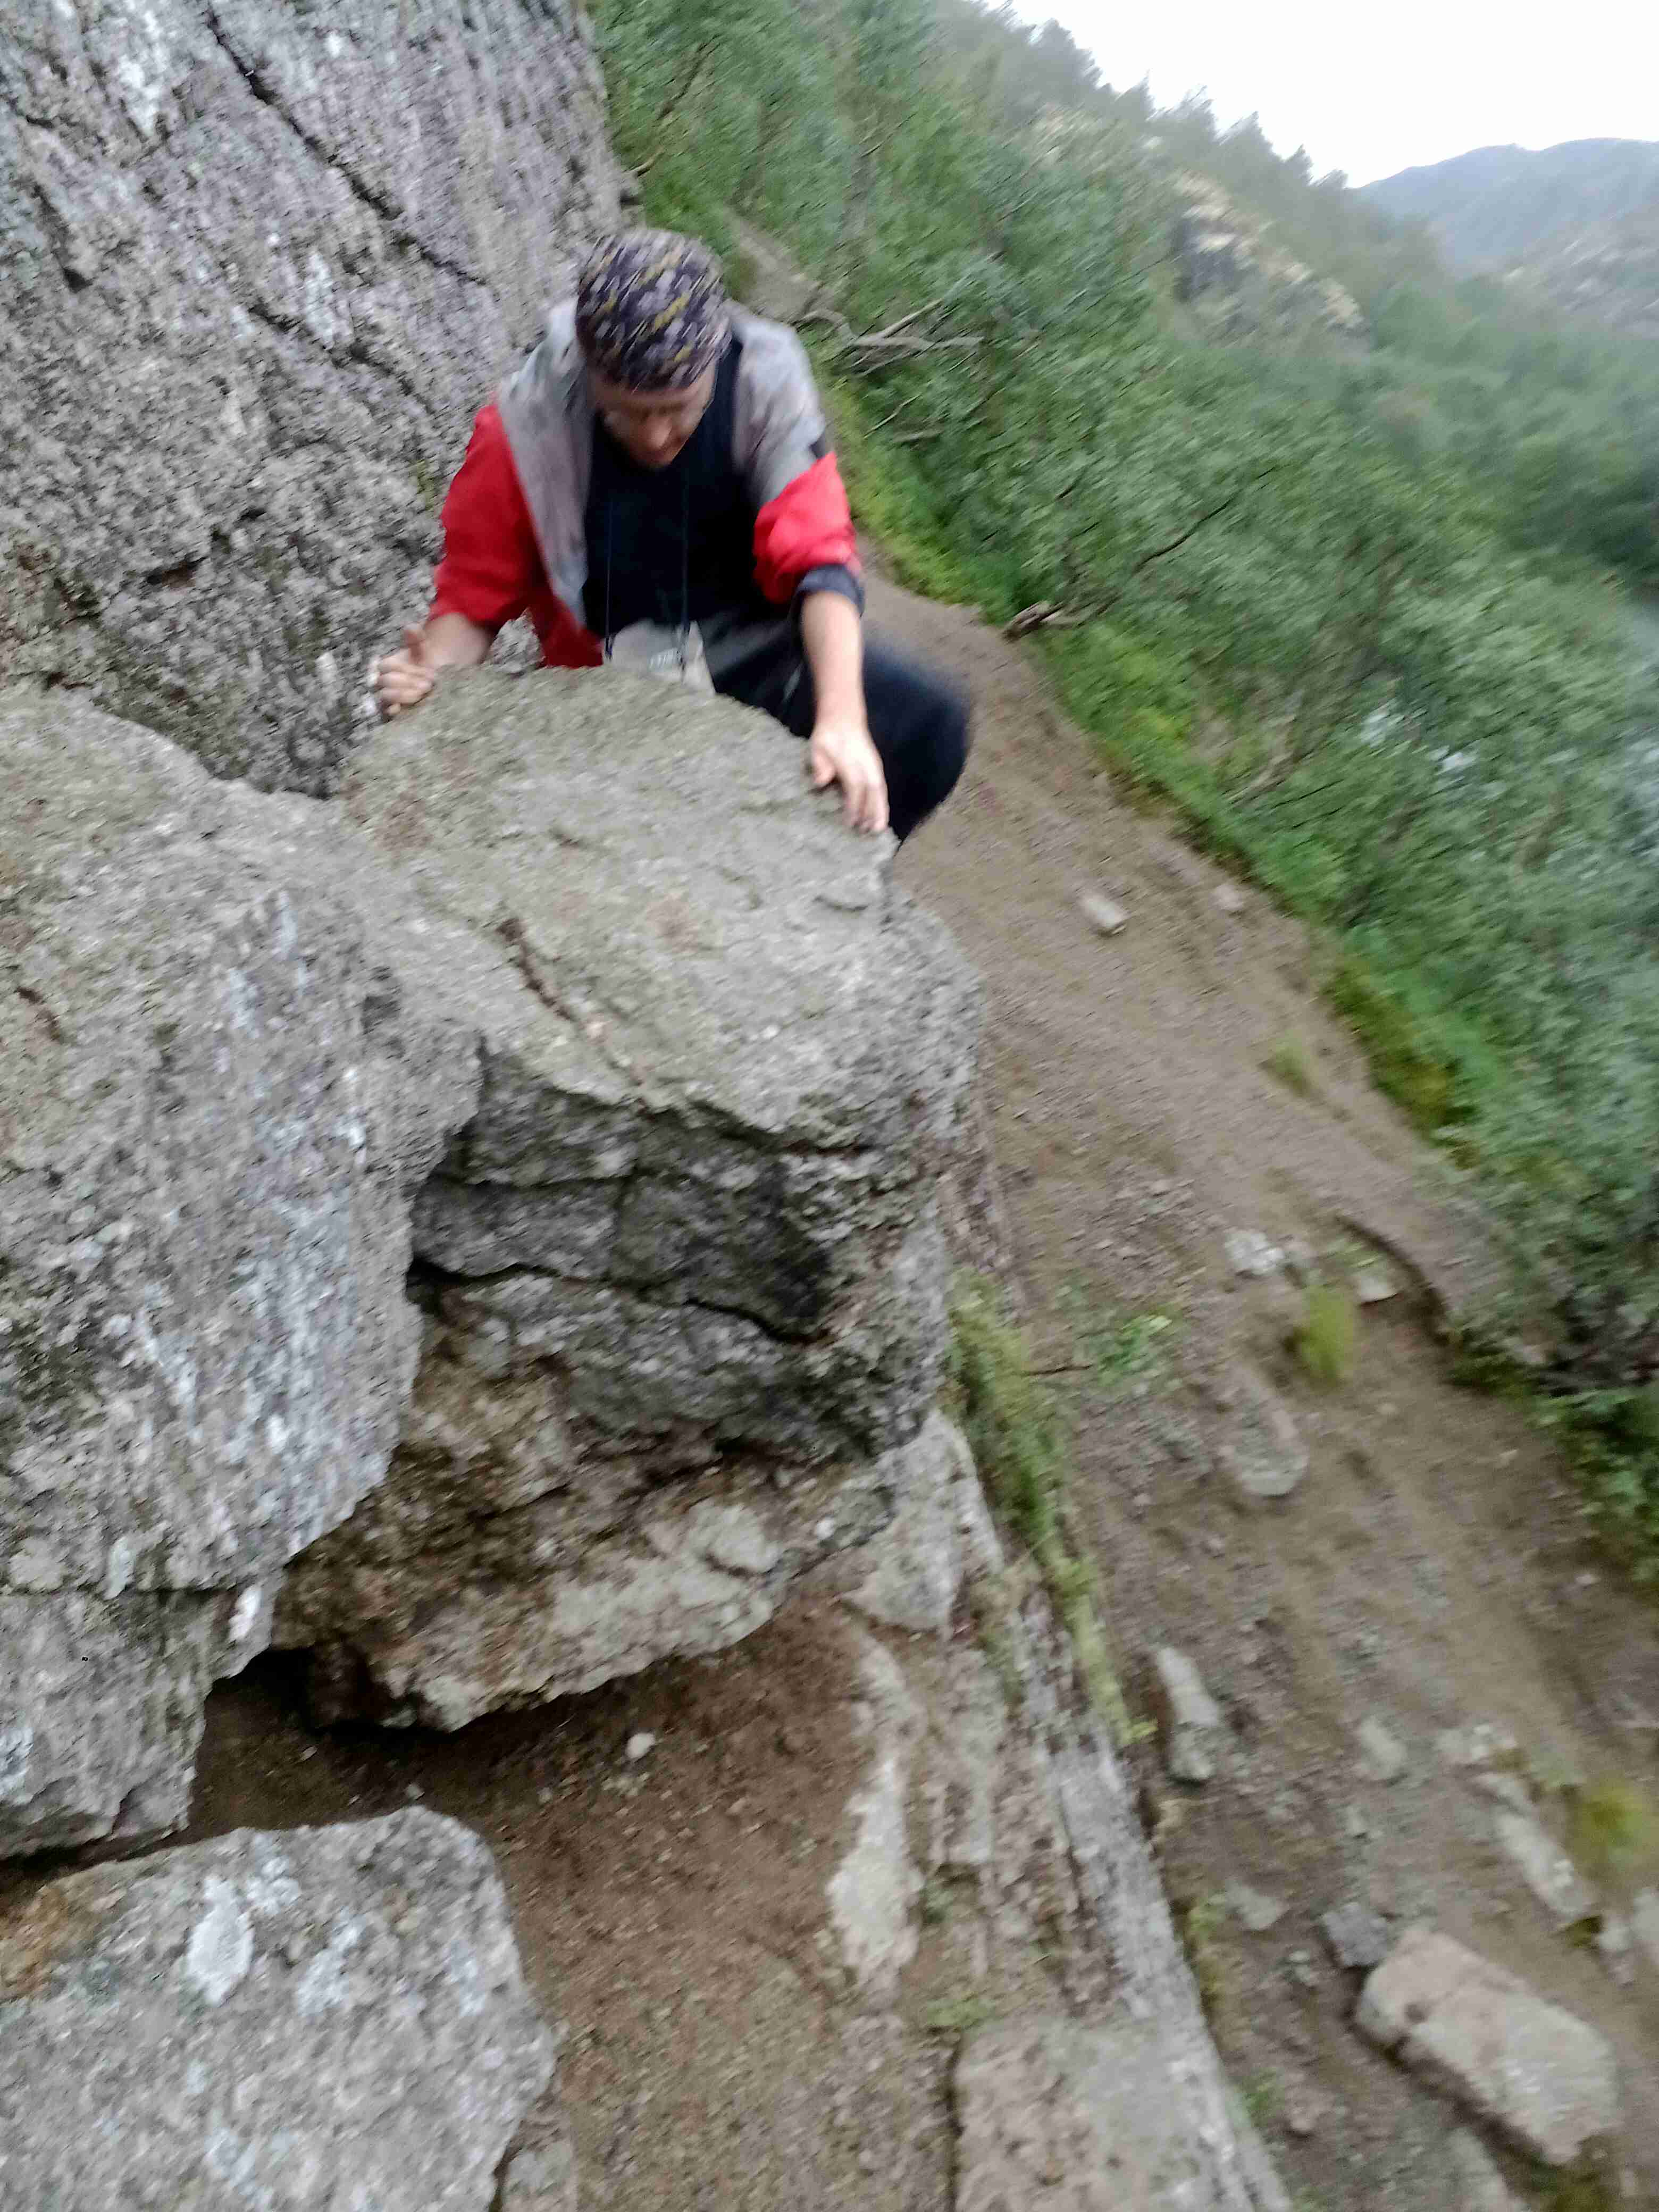
\includegraphics[width=14cm]{foto/06_08/02.Камень на полочке.png.jpg}
    \caption{Камень на скальной полке}
    \label{fig2:2}
\end{figure}

\begin{figure}
    \centering
    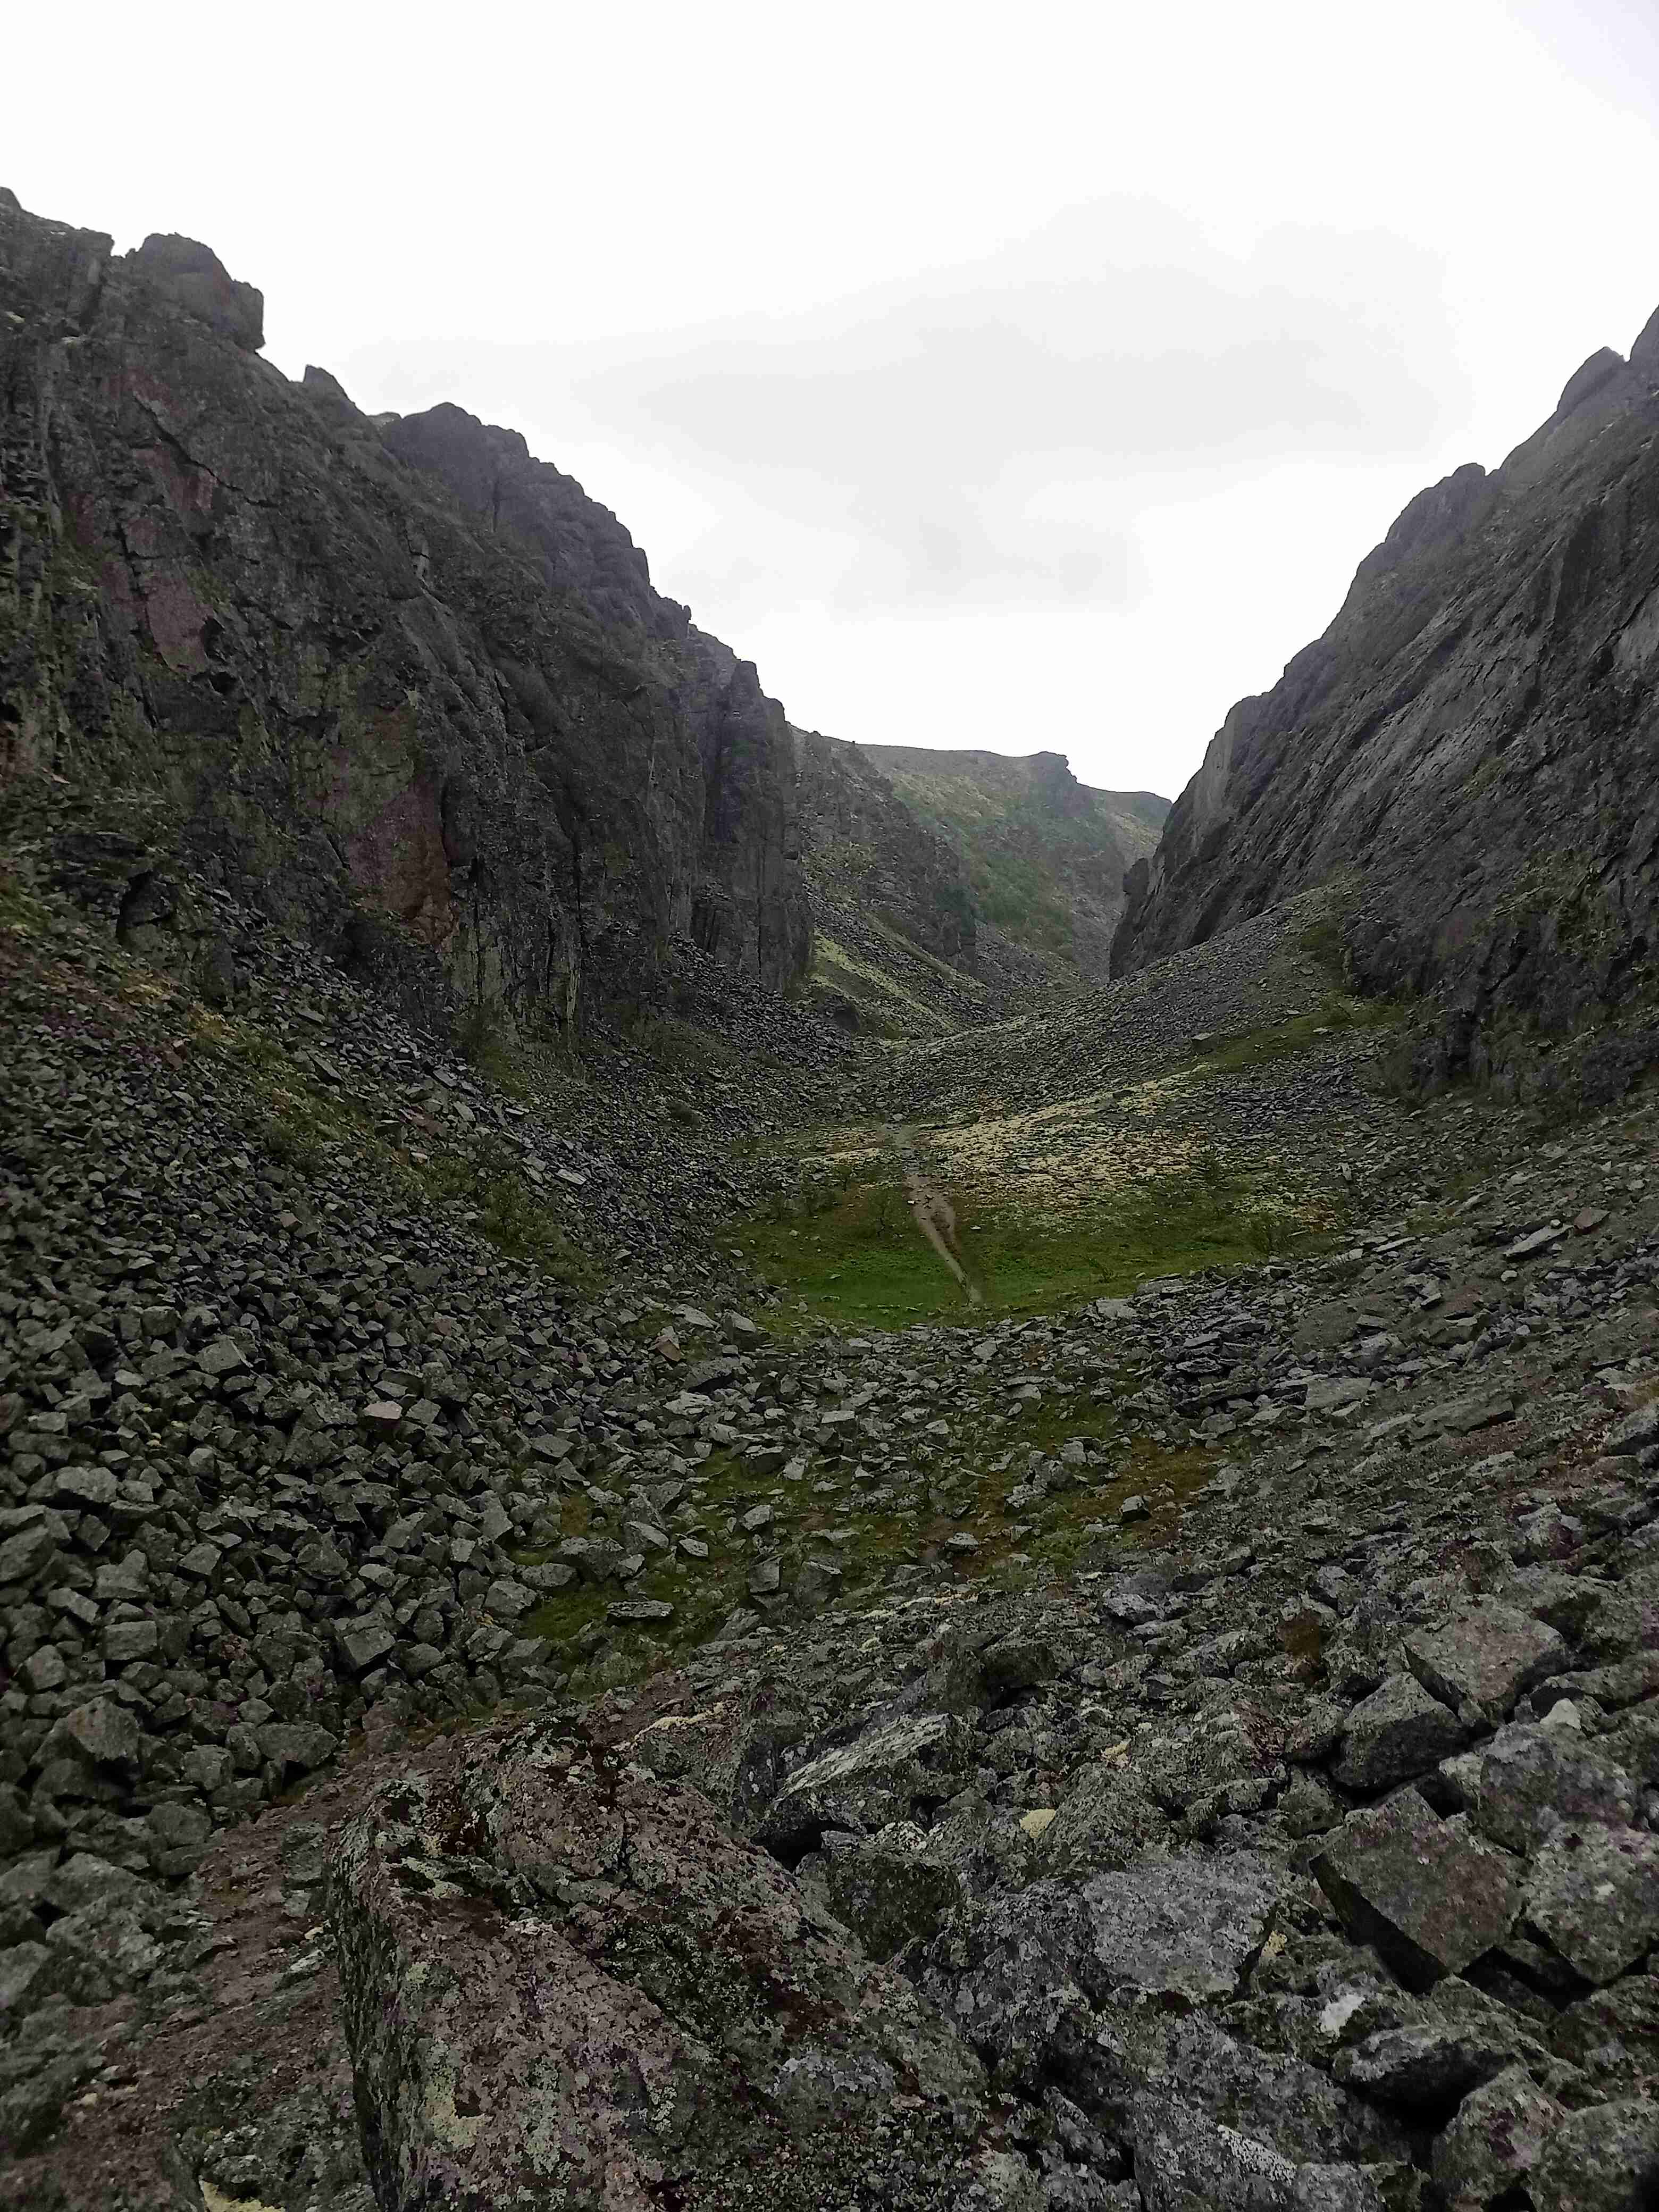
\includegraphics[width=14cm]{foto/06_08/03.Ущелье Аку-Аку.png.jpg}
    \caption{Ущ. Аку-Аку}
    \label{fig2:3}
\end{figure}

\begin{figure}
    \centering
    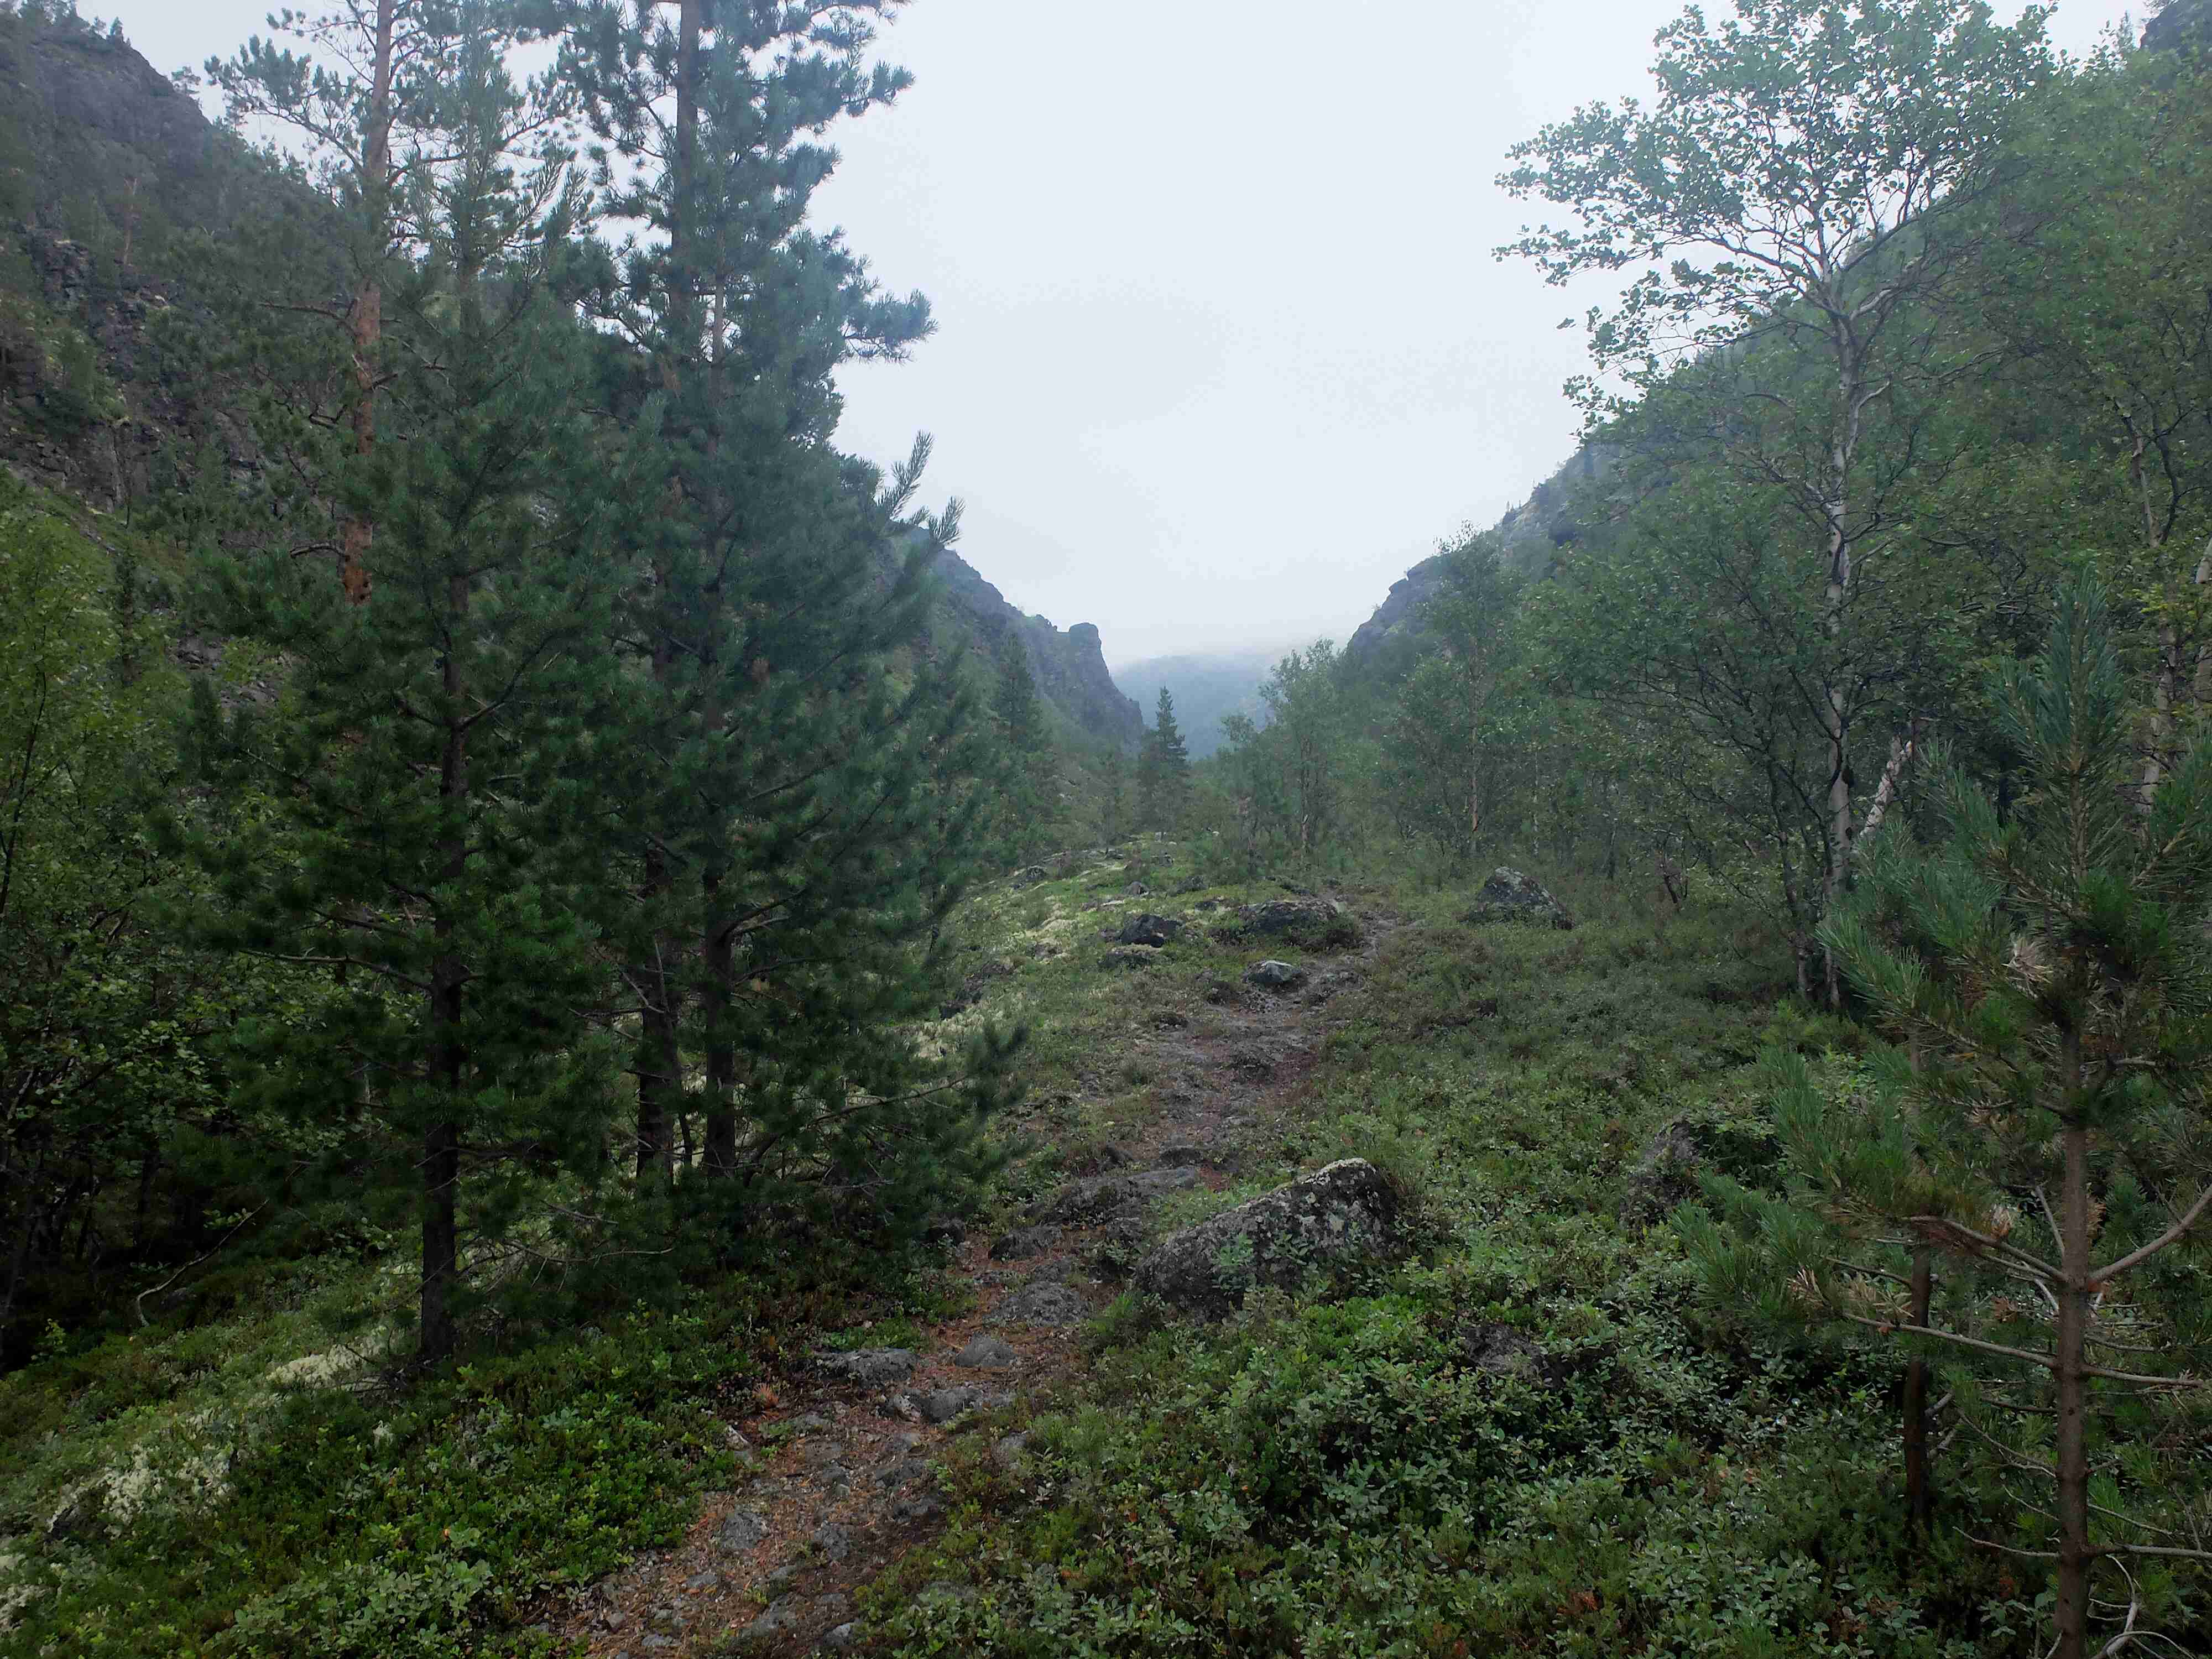
\includegraphics[width=14cm]{foto/06_08/05.Ущелье Звёздочка.png.jpg}
    \caption{Ущ. Звёздочка}
    \label{fig2:4}
\end{figure}

\FloatBarrier

\subsection{День 3. 07.08.2022\\
Руч. Медвежий Лог -- пер. Медвежий Лог (н/к, 790 м) -- руч. Чильмана -- р. Малая Белая}
\begin{tabular}{l p{12cm}}
\hline
Пройдено: & 9.67 км\\
Набор/сброс высоты: & 554/583 м\\
Время в пути: & 9:15\\
ЧХВ: & 4:48\\
Метеоусловия: & Днём --- пасмурно, временами дождь.\hfill \break Вечером --- переменная облачность.\\
\hline
\end{tabular}

Ночью попеременно шёл дождь. Около 6 часов утра облака над долиной вниз по течению руч. Медвежий Лог разошлись,
потом снова затянуло.

08:10 Подъём, пасмурно, +16.5$\tccentigrade$.

10:00 Выход.
Со стоянки к перевалу уходит исчезающая лесная тропа, поэтому часть времени идём просто ориентируясь на ручей (рис. \ref{fig3:1}),
в любом случае, лес скоро кончается. Пару раз перепрыгиваем через ручей туда-сюда.
Через 1.3 километра ручей разделяется на два притока, тот который уходит на юг ведёт к нашему перевалу.
Левый (орогр.) берег притока совсем крутой, правый положе. Но мы всё равно решает срезать и идти не по правому берегу,
а взять левее (по напр. дв.) и  пойти по травянистому склону холма. В итоге холм оказывается склоном долины ручья,
который поднимается вместе с ручьём, а чтобы пойти на перевал приходится сначала спуститься к ручью.

Около 11 приходим под перевал. На склоне чётко видны 3 расщелины, по виду каменистые, скользкие и, кажется, с ручейками.
Решаем идти за третьей (самая левая по напр. дв), выдвигаемся (рис. \ref{fig3:2}). Характер склона --- сыпуха, живые камни, трава,
скользкий мох, скальные выступы. Поднимаемся около 50 минут. Выходим сбоку от ущелья перевала, сверху.
Красиво и мрачно. За пару минут чуть-чуть спускаемся назад, чтобы войти в ущелье 12:21.

Это перевал тектонического происхождения и тоже состоит из нескольких камер (рис. \ref{fig3:3}). В первой --- снежник.
В одной из центральных камер находим тур, но тот пустой. Накрапывает дождь. У восточного выхода расположено
небольшое озерцо (рис. \ref{fig3:4}), где-то над ним должен был быть ещё один тур, но мы про него забыли.

Тут нас накрывает облако. Куда идти не видно. Залезаем от ветра в трещину, съедаем перевальную шоколадку.
Неподвижно сидеть становится холодно, решаем переждать низкую облачность в палатке, находим место на одну палатку
у восточного берега озерца. 13:29, ставимся, готовим обед в палатке. Один раз ненадолго проясняется,
но почти сразу снова затягивает. Наконец облака уходят, видимость до Имандры, а главное видно как спускаться (рис. \ref{fig3:5}).
Сворачиваемся в быстром темпе, фотографируемся и уходим 16:37.
Вниз ведёт тропа: сыпуха, средние камни, мох, сыпуха глиссером. Тропа спускается к руч. Чильмана и пропадает (рис. \ref{fig3:6}).
Переходим на левый берег ручья. Входим в лес, по лесной тропе доходим до дороги вдоль р. Малой Белой.
Дорога вездеходная, проходит через лес. Идём по ней до руч. Ферсмана. Много стоянок, но и людей много.
Переходим ручей по бревну, становимся на поляне у впадения Ферсмана в Малую Белую 19:15.

Распогодилось: облачно с солнцем, закатный свет солнца красиво освещает горный склон с противоположной стороны реки.
Мы тем временем ужинаем, сушимся, стираемся.

21:30 отбой.

\begin{figure}
    \centering
    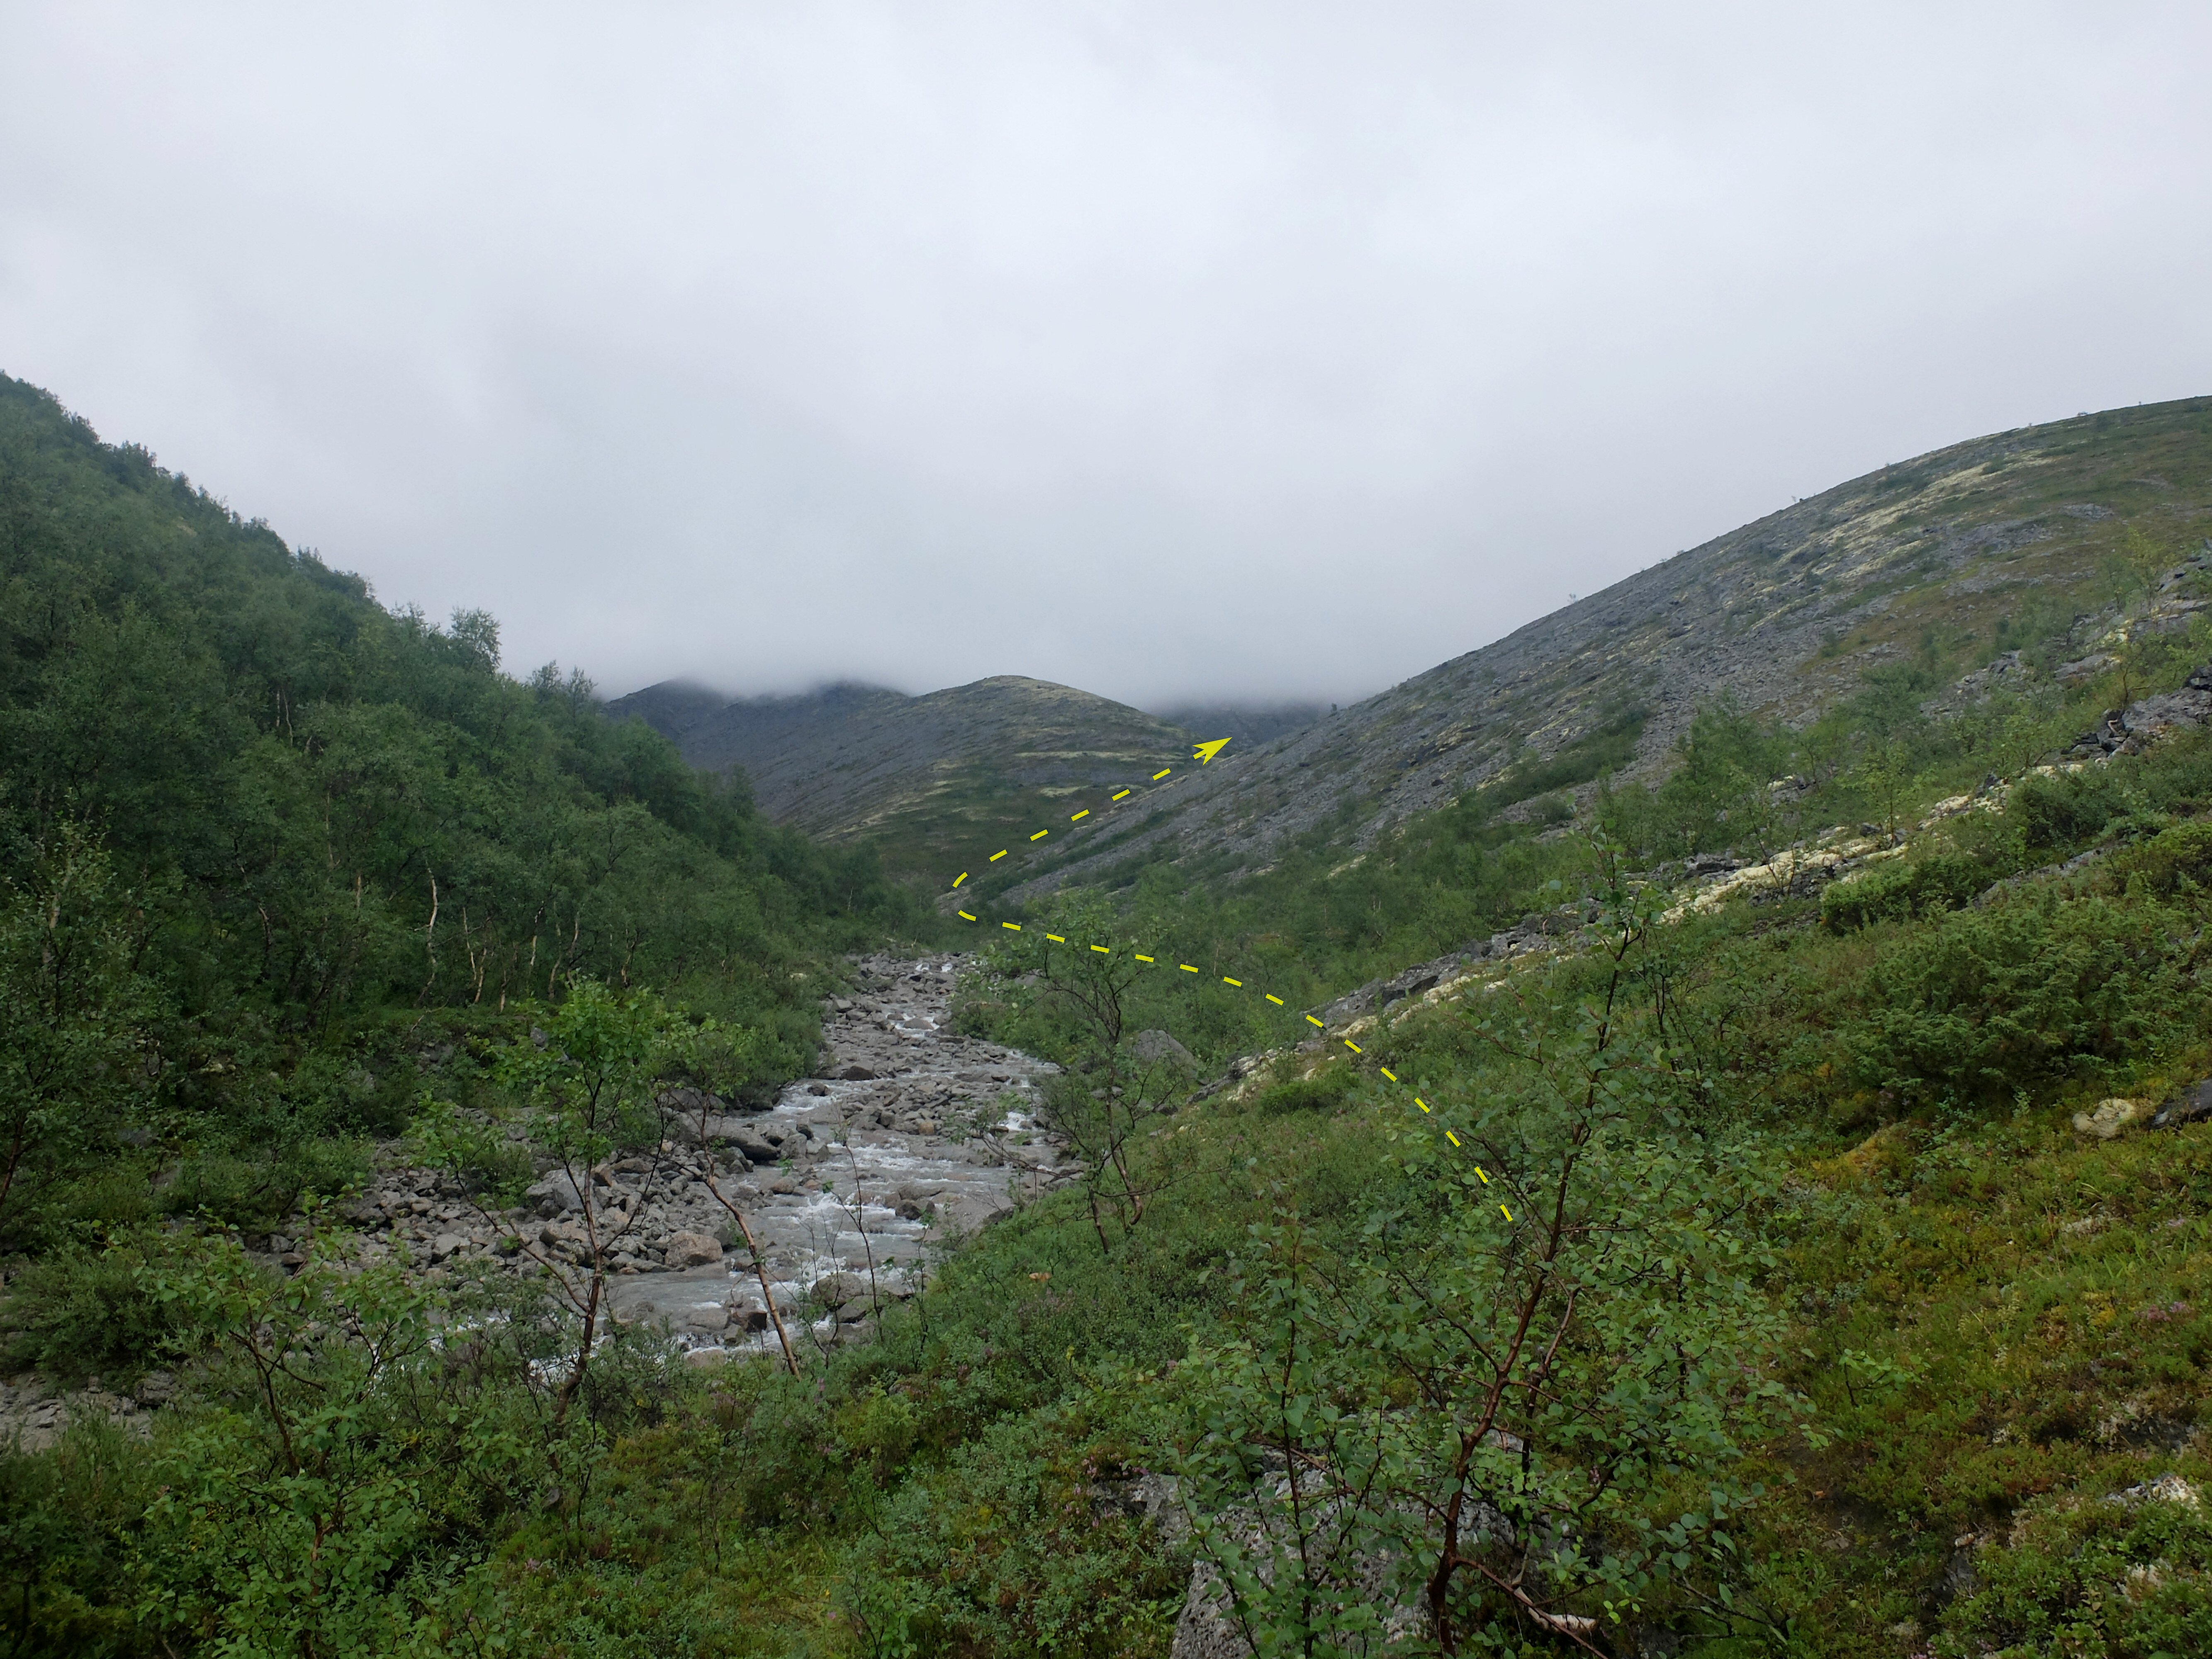
\includegraphics[width=14cm]{foto/07_08/01.Путь по ручью.png.jpg}
    \caption{Путь по ручью к пер. Медвежий Лог}
    \label{fig3:1}
\end{figure}

\begin{figure}
    \centering
    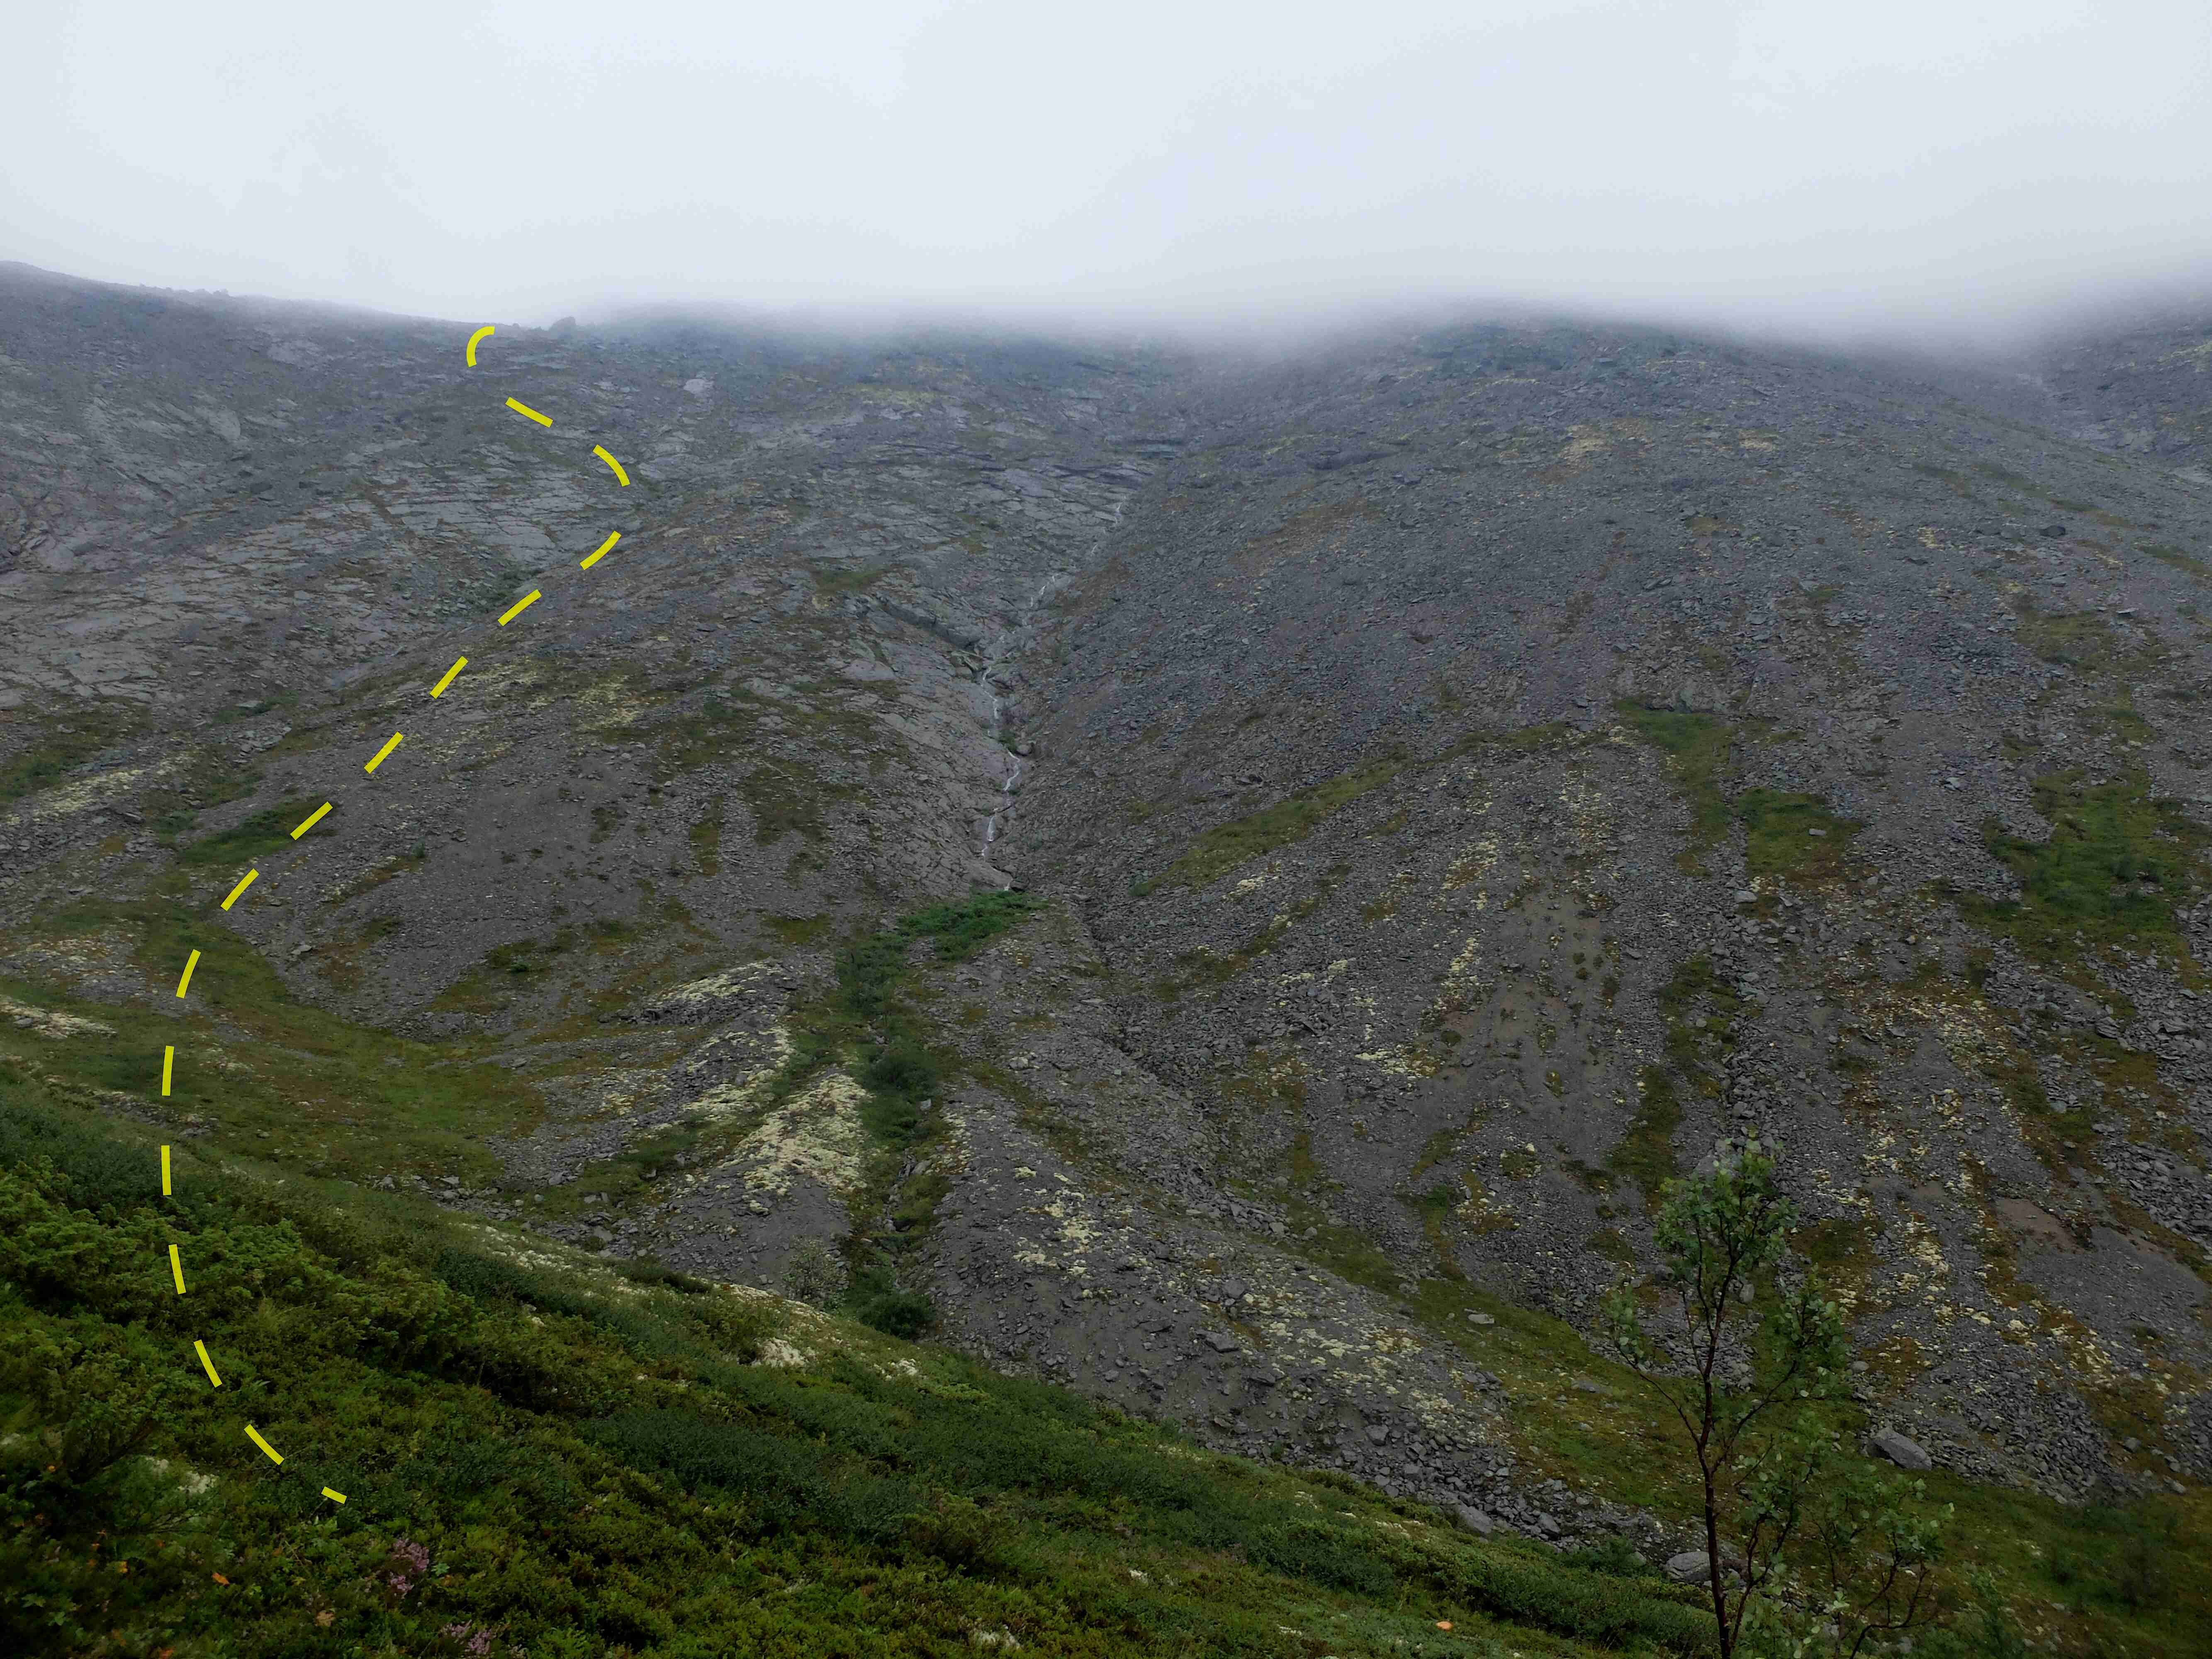
\includegraphics[width=14cm]{foto/07_08/01.2. Подъем к перевалу.png.jpg}
    \caption{Подъём на пер. Медвежий Лог}
    \label{fig3:2}
\end{figure}

\begin{figure}
    \centering
    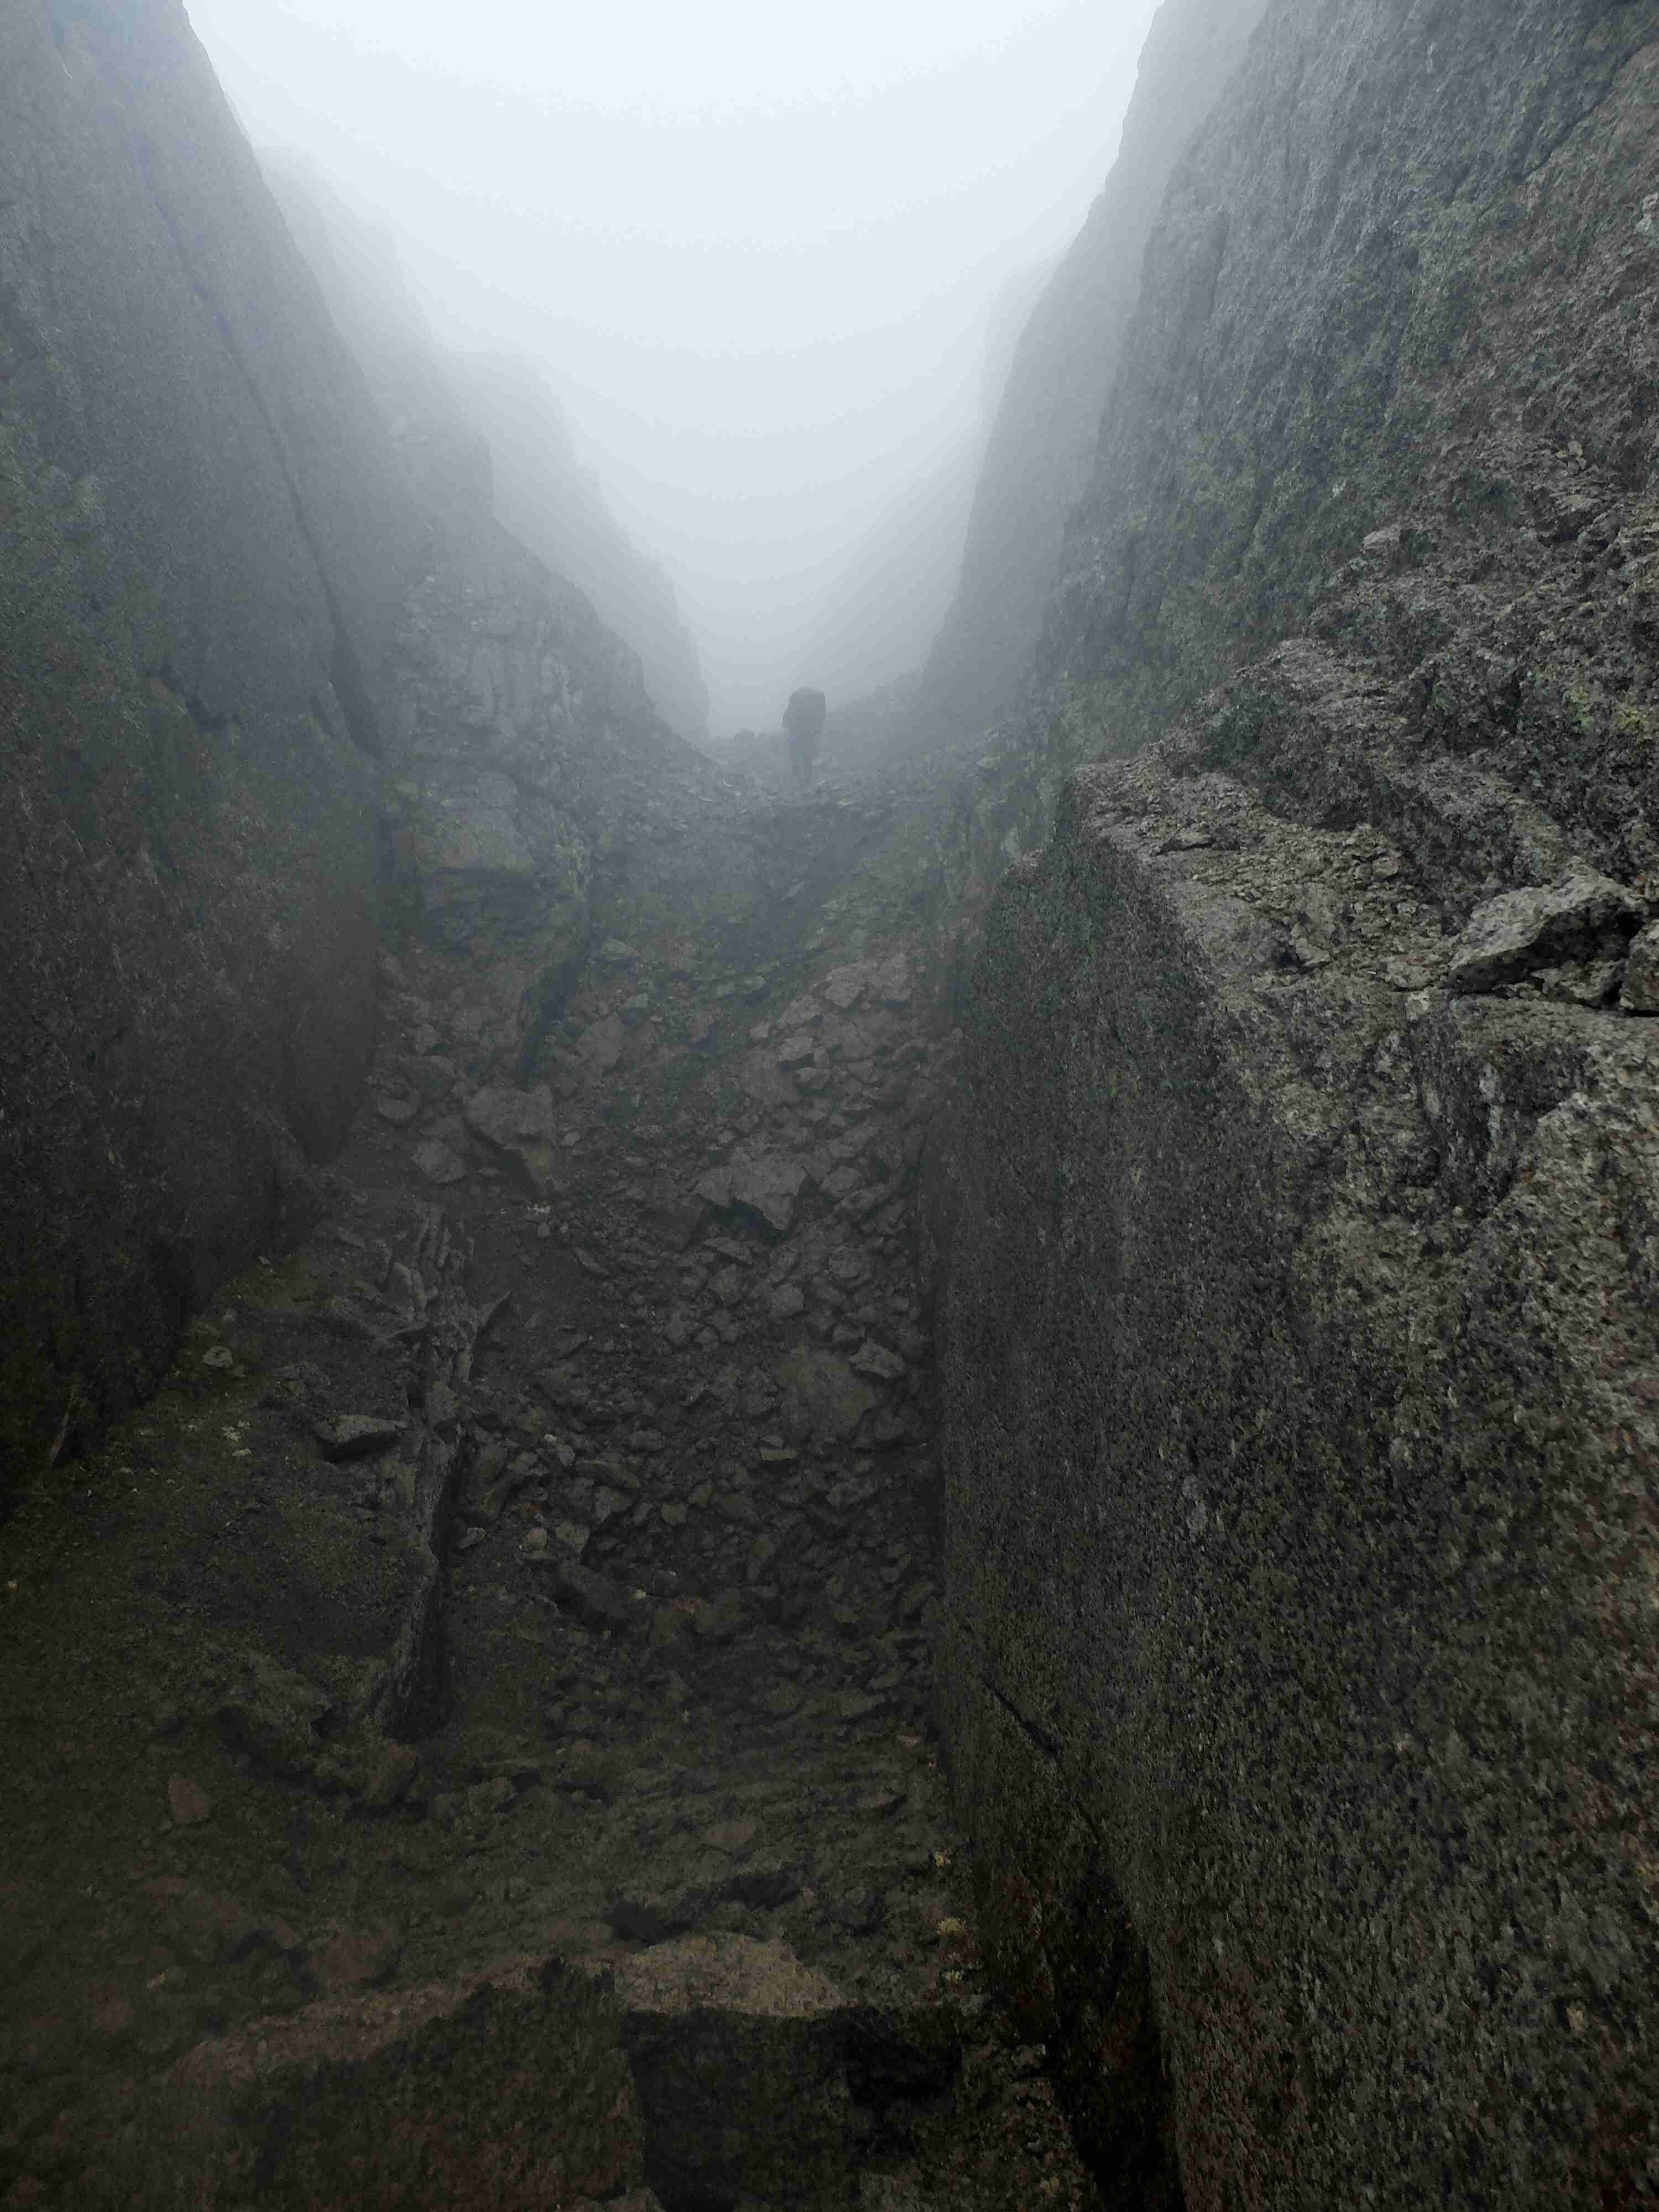
\includegraphics[width=14cm]{foto/07_08/02.Расщелина перевала.png.jpg}
    \caption{Расщелина пер. Медвежий Лог}
    \label{fig3:3}
\end{figure}

\begin{figure}
    \centering
    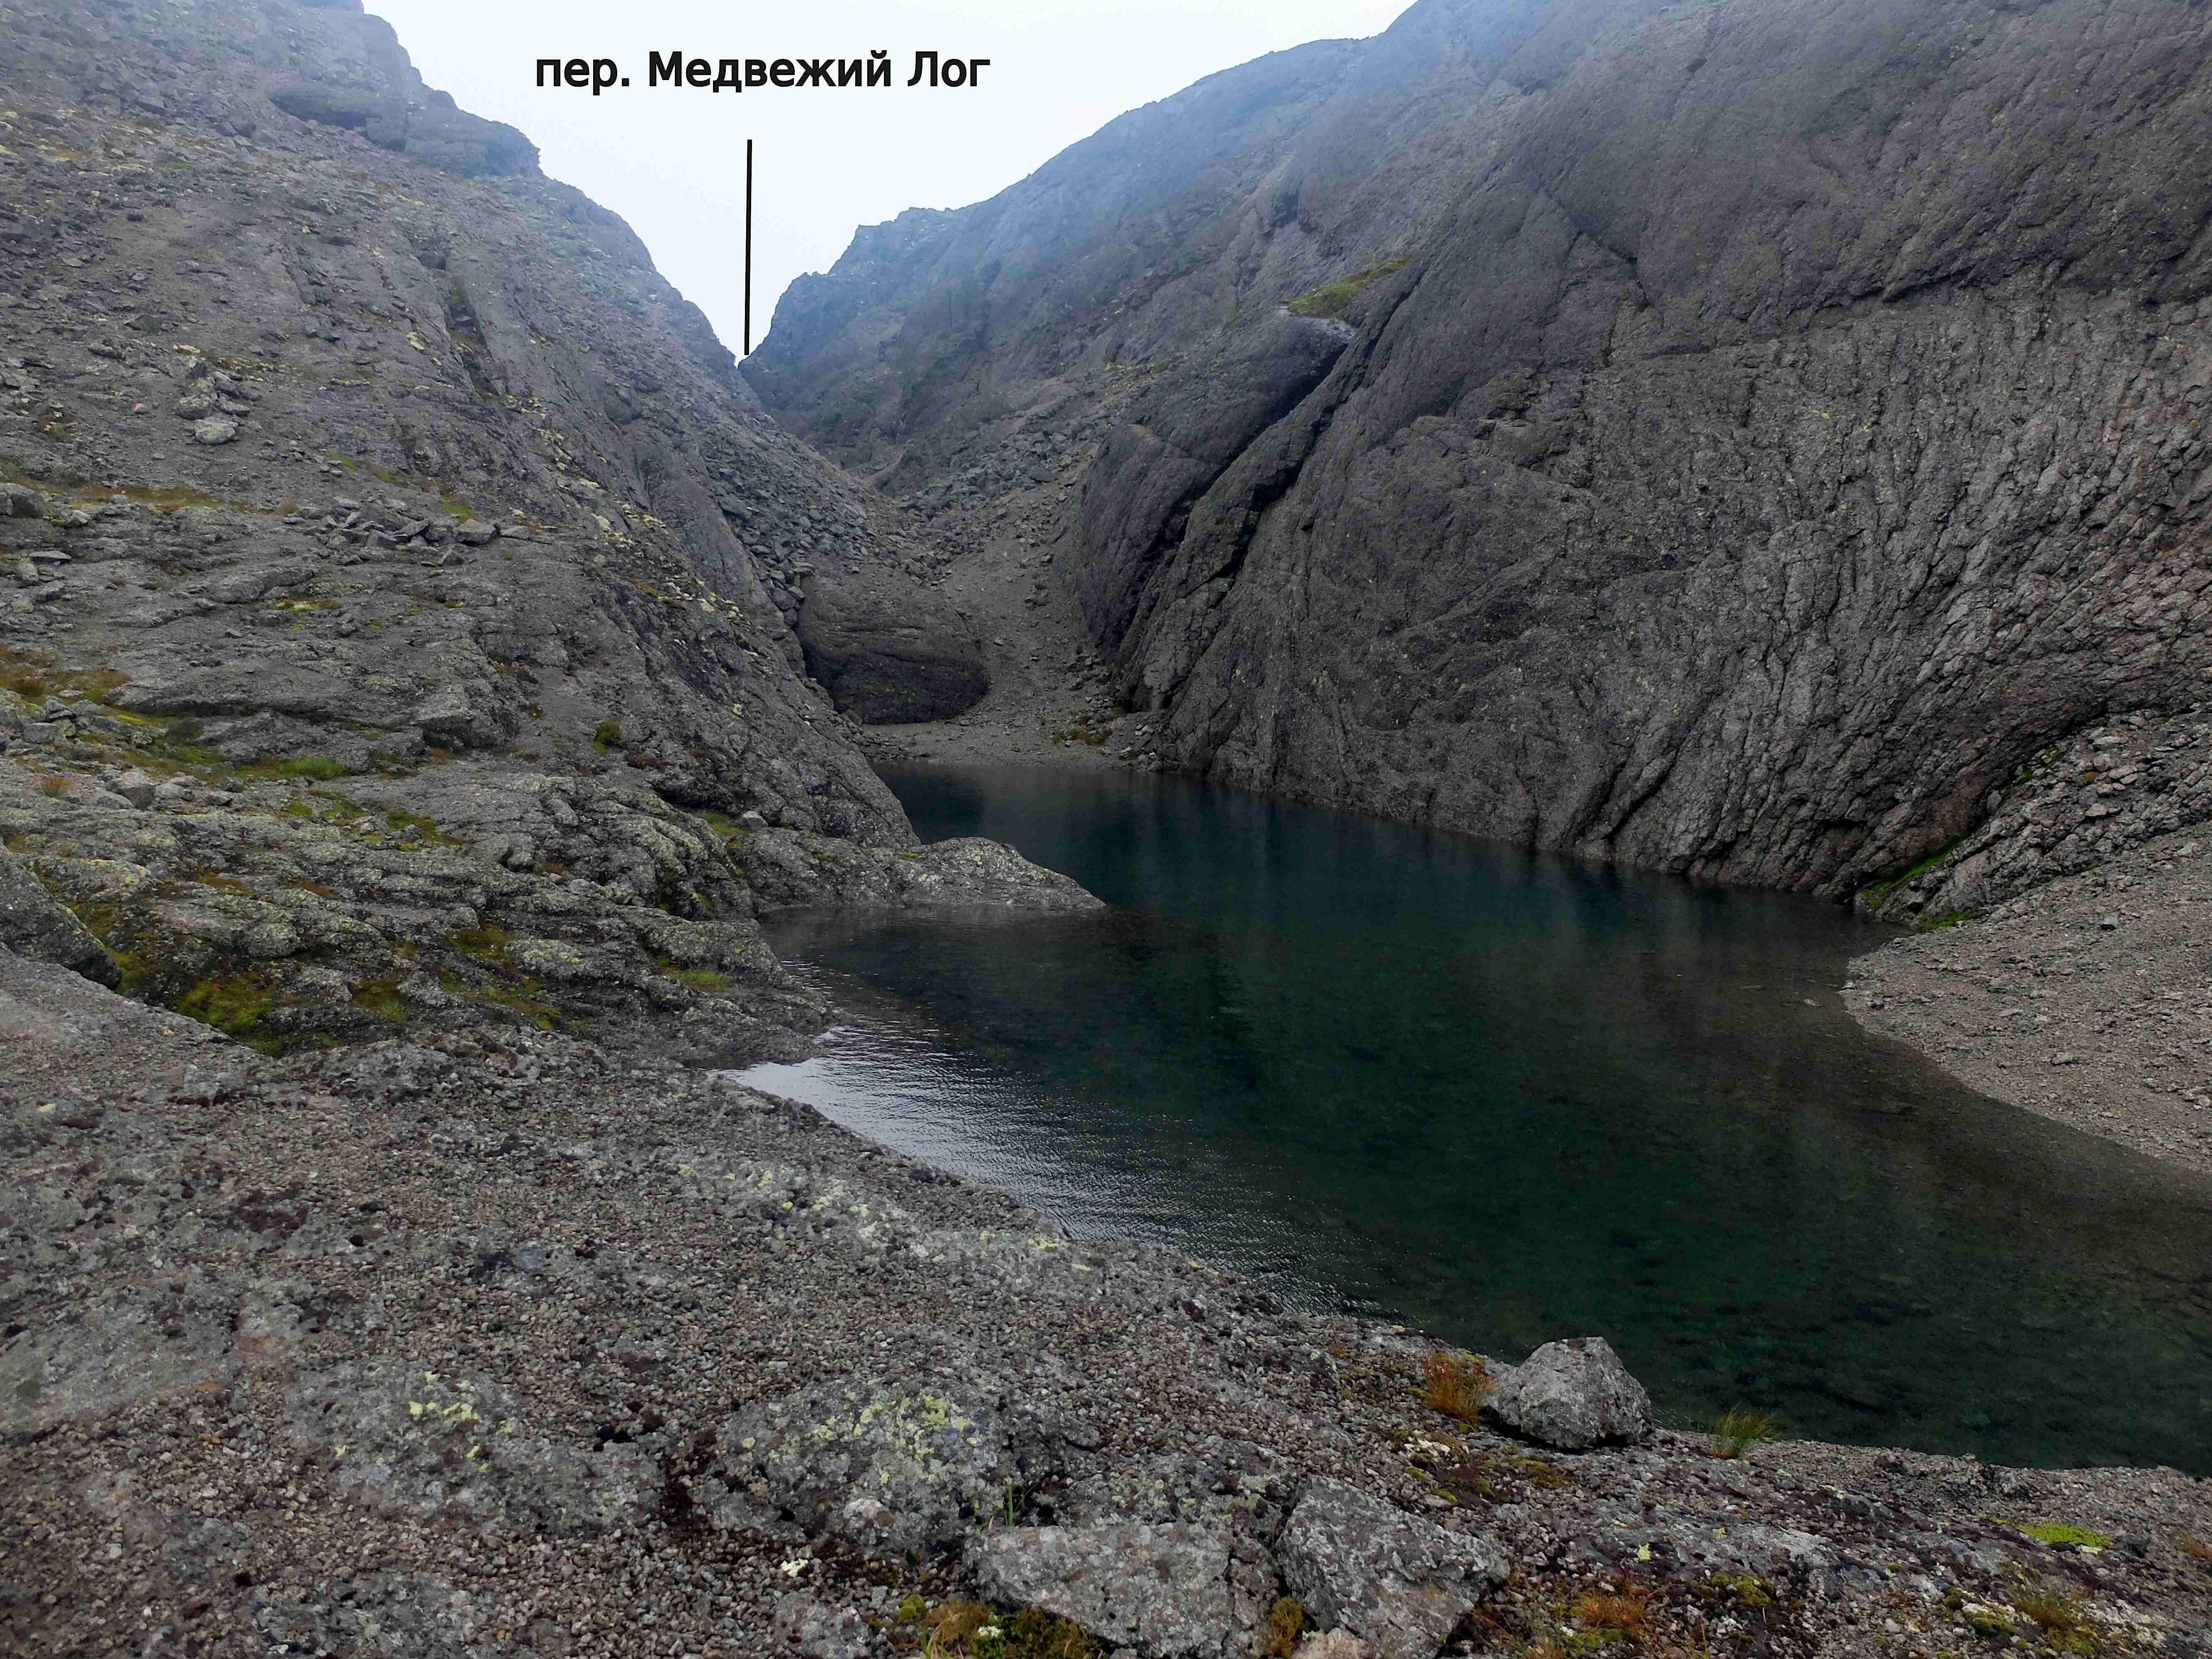
\includegraphics[width=14cm]{foto/07_08/03.Вид на перевал и озеро с юга.png.jpg}
    \caption{Вид на озеро и пер. Медвежий Лог с юга}
    \label{fig3:4}
\end{figure}

\begin{figure}
    \centering
    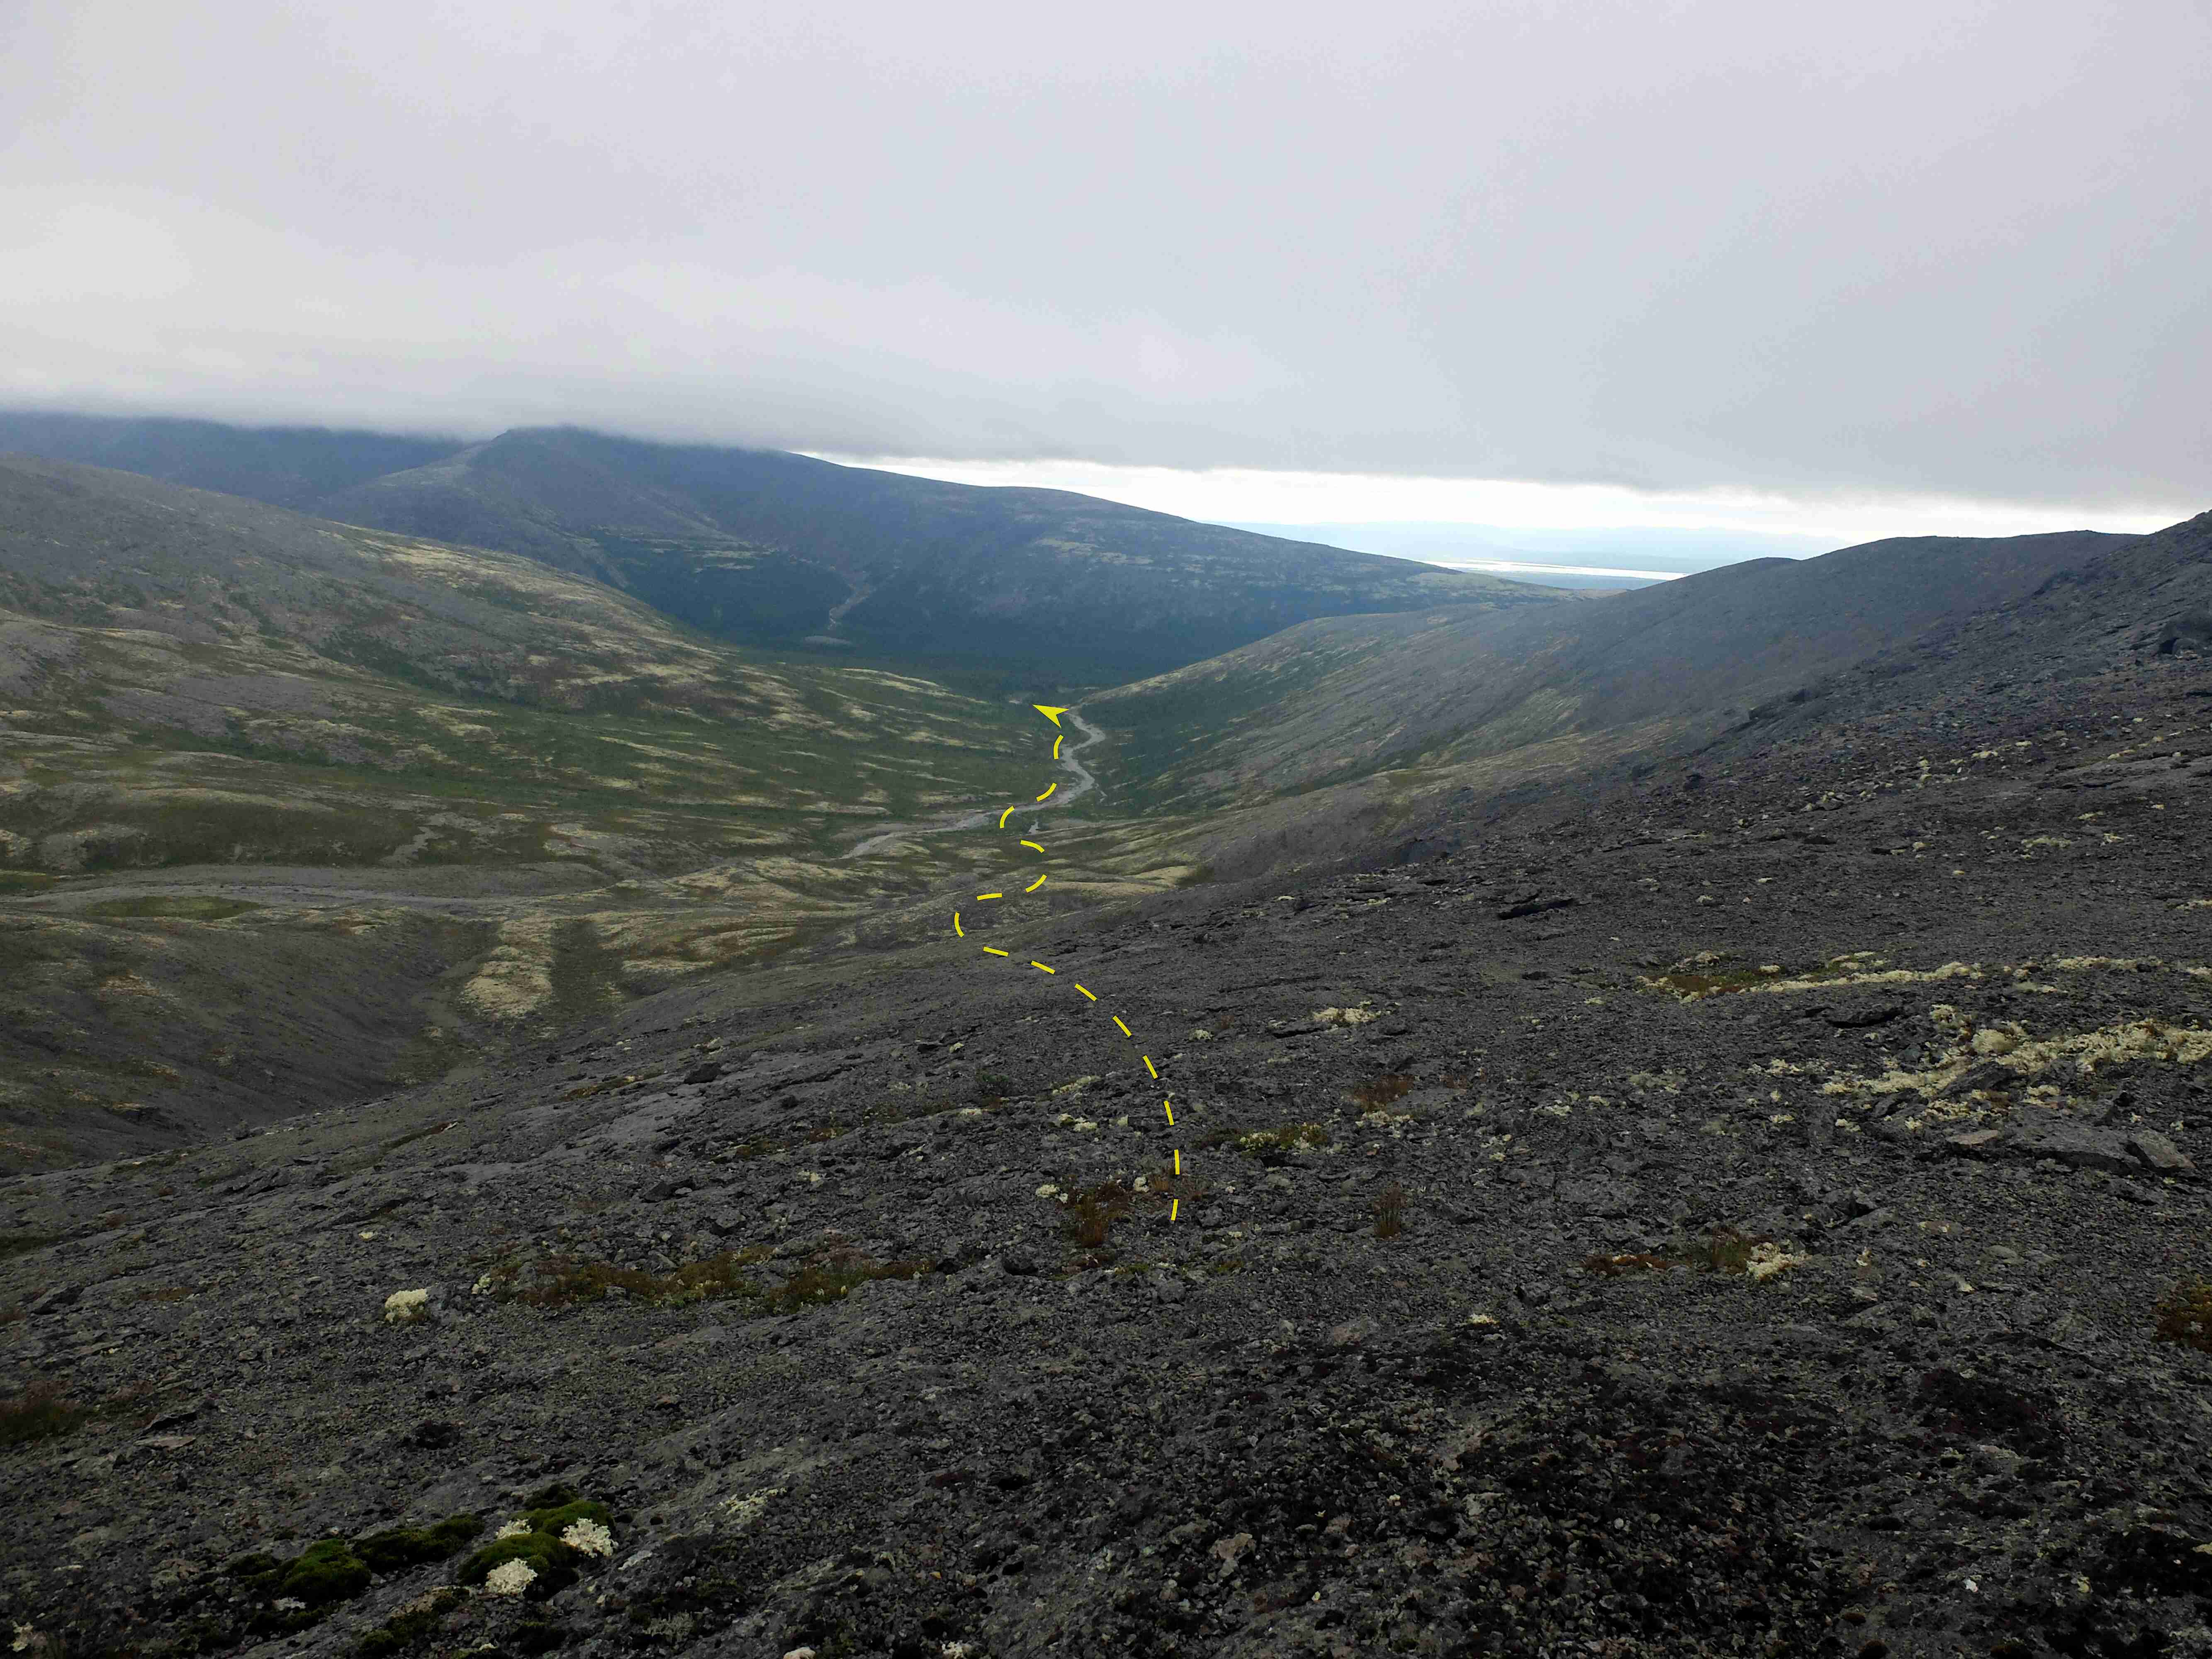
\includegraphics[width=14cm]{foto/07_08/04.Спуск с перевала в долину реки Белой.png.jpg}
    \caption{Спуск с пер. Медвежий Лог в долину р. Малой Белой}
    \label{fig3:5}
\end{figure}

\begin{figure}
    \centering
    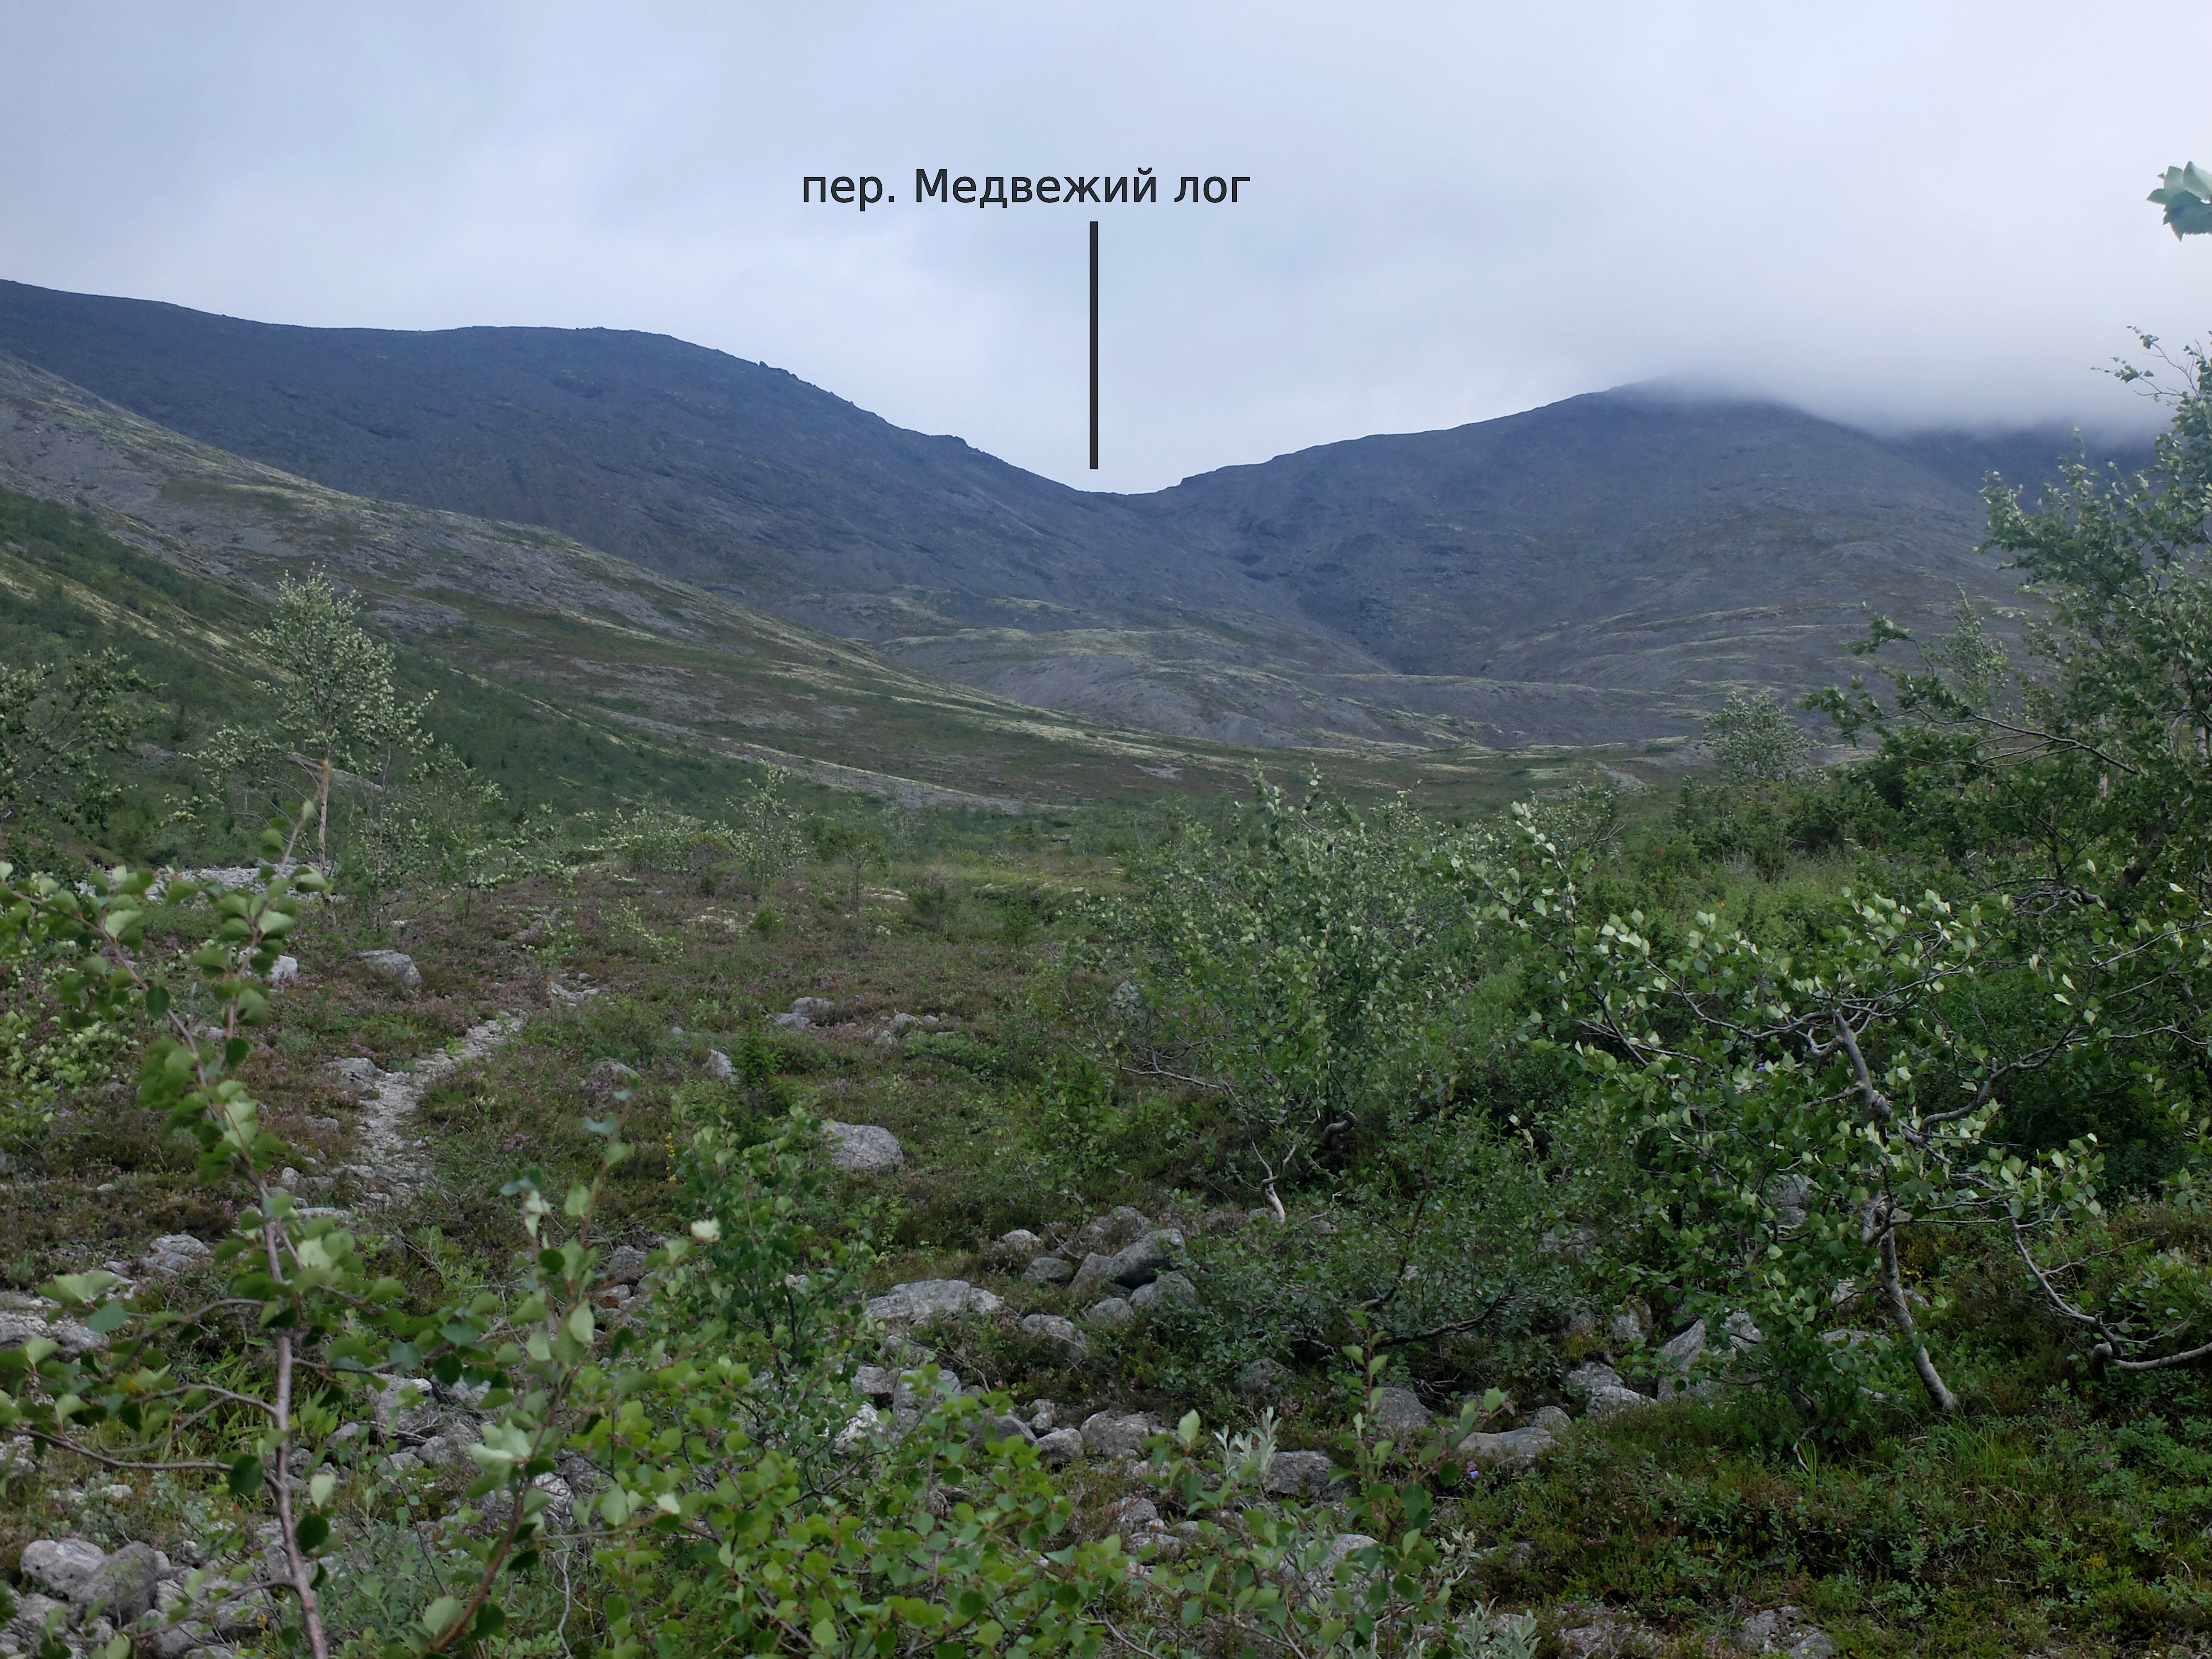
\includegraphics[width=14cm]{foto/07_08/05.Вид на перевал медвежий лог с юга.png.jpg}
    \caption{Вид на пер. Медвежий Лог с юга}
    \label{fig3:6}
\end{figure}

\FloatBarrier

\subsection{День 4. 08.08.2022\\
Р. Малая Белая -- пер. Петрелиуса Западный (н/к, 850 м) -- руч. Петрелиуса}
\begin{tabular}{l p{12cm}}
\hline
Пройдено: & 15.8 км\\
Набор/сброс высоты: & 719/719 м\\
Время в пути: & 8:49\\
ЧХВ: & 5:44\\
Метеоусловия: & Первая половина дня --- пасмурно, временами дождь.\hfill \break После перевала --- переменная облачность.\\
\hline
\end{tabular}\\

08:00 Подъём.
Облачно с прояснениями, иногда солнце, +15$\tccentigrade$

10:07 Выходим.
Идём по вчерашней вездеходной дороге. Вскоре лес редеет и сменяется сначала травянистой растительностью, потом мхом.
В районе оз. Тахтаръявр дорога заканчивается, далее идём по тропе (рис. \ref{fig4:1}).
Проходим ответвление на пер. Рамзая. Через 700 метров у развилки на пер. Петрелиуса Восточный и Западный
должно быть озерцо (\enquote{Хэмингуэ}), но оно пересохло. В маршрутной книжке это озерцо записано как место ночёвки,
но выйдя из МКК, руководитель вспомнил о его непостоянной природе, поэтому если бы мы не отстали по времени,
то всё равно заночевали бы не здесь, а около оз. Тахтаръявр.
От озера отворот на Петрелиуса Западный. Петрелиуса Восточный в облаке, хорошо что нам не туда.

12:57 Начинаем подъём. Мох заканчивается, дальше в основном курумник, склон положе чем у вчерашнего пер. Медвежий Лог,
идём по турикам (рис. \ref{fig4:2}). При подходе к перевалу видим ещё одну поднимающуюся группу из трёх человек.

13:37 Последний на нашем маршруте разломный перевал (рис. \ref{fig4:3}). Несколько камер. Три снежника.
В сами камеры не спускаемся,
тропы там не видно, идём по курумнику левого склона. На выходе --- почти плато, с небольшим наклоном,
камень с памятным знаком Петрелиусу, слева --- монументальный цирк, на стенах цирка хорошо видно
работу ледника --- как ножом срезано, у подножия цирка --- голубое озеро (рис. \ref{fig4:4}).

Поскольку идущая перед нами группа не заинтересовалась туром (мы спрашивали), то забираем записку группы из
Нижнего Новгорода (руководитель не указан, первый в списке Смирнов Иван) от 07.08.2022 (рис. \ref{fig:zapiski2}), оставляем свою.

14:09 Начинаем спуск, видно две явных тропки, выбираем левую, по правой спускается группа перед нами.
Крутизна склона с этой стороны больше чем на подъёме. Сама тропка с мелкими камнями.

14:37 Спустились к озеру, нашли искусственную стенку, спрятались за ней от ветра и стали на обед.
Вдали, не спускаясь к нашему озеру, на перевал проходит огромная группа с рюкзаками.
Пока обедаем они почти поднимаются на перевал. Видимо наша записка попадёт к ним (рис. \ref{fig4:5}).

16:07 Выходим.
Идём по правому берегу руч. Петрелиуса, озёра каскадом, тропа, турики вдоль тропы (рис. \ref{fig4:6}).
Склон горы Петрелиуса заканчивается, основная тропа уходит на север. На карте, со стороны пер. Петрелиуса Восточный
показана хорошая дорога, к тому же она идёт выше и менее лесиста, есть надежда быть менее покусанными комарами.
Решаем, что \enquote{лучше за пять минут} долететь и сворачиваем к ней.
Подъём длиной метров 350, и действительно --- дорога с широкой колеёй вездехода. Дорога холмистая: то вверх, то вниз.

18:57 Доходим до места стоянки. Стоянок много. И никого.
На противоположном берегу по карте тоже много стоянок. И кто-то шумный, но к нам так просто не подобраться --- удобного брода нет.

Стоянку охраняет деревянный истукан, который собирает за нерадивыми туристами консервные банки и ботинки (рис. \ref{fig4:7}).

Ужинаем. Далее личное время.
Вокруг куча ягод. Рядом очень прекрасный тра\-вя\-ни\-сто-бо\-ло\-тис\-тый луг, с тропками по которым можно гулять.

23:20 отбой летописца

\begin{figure}
    \centering
    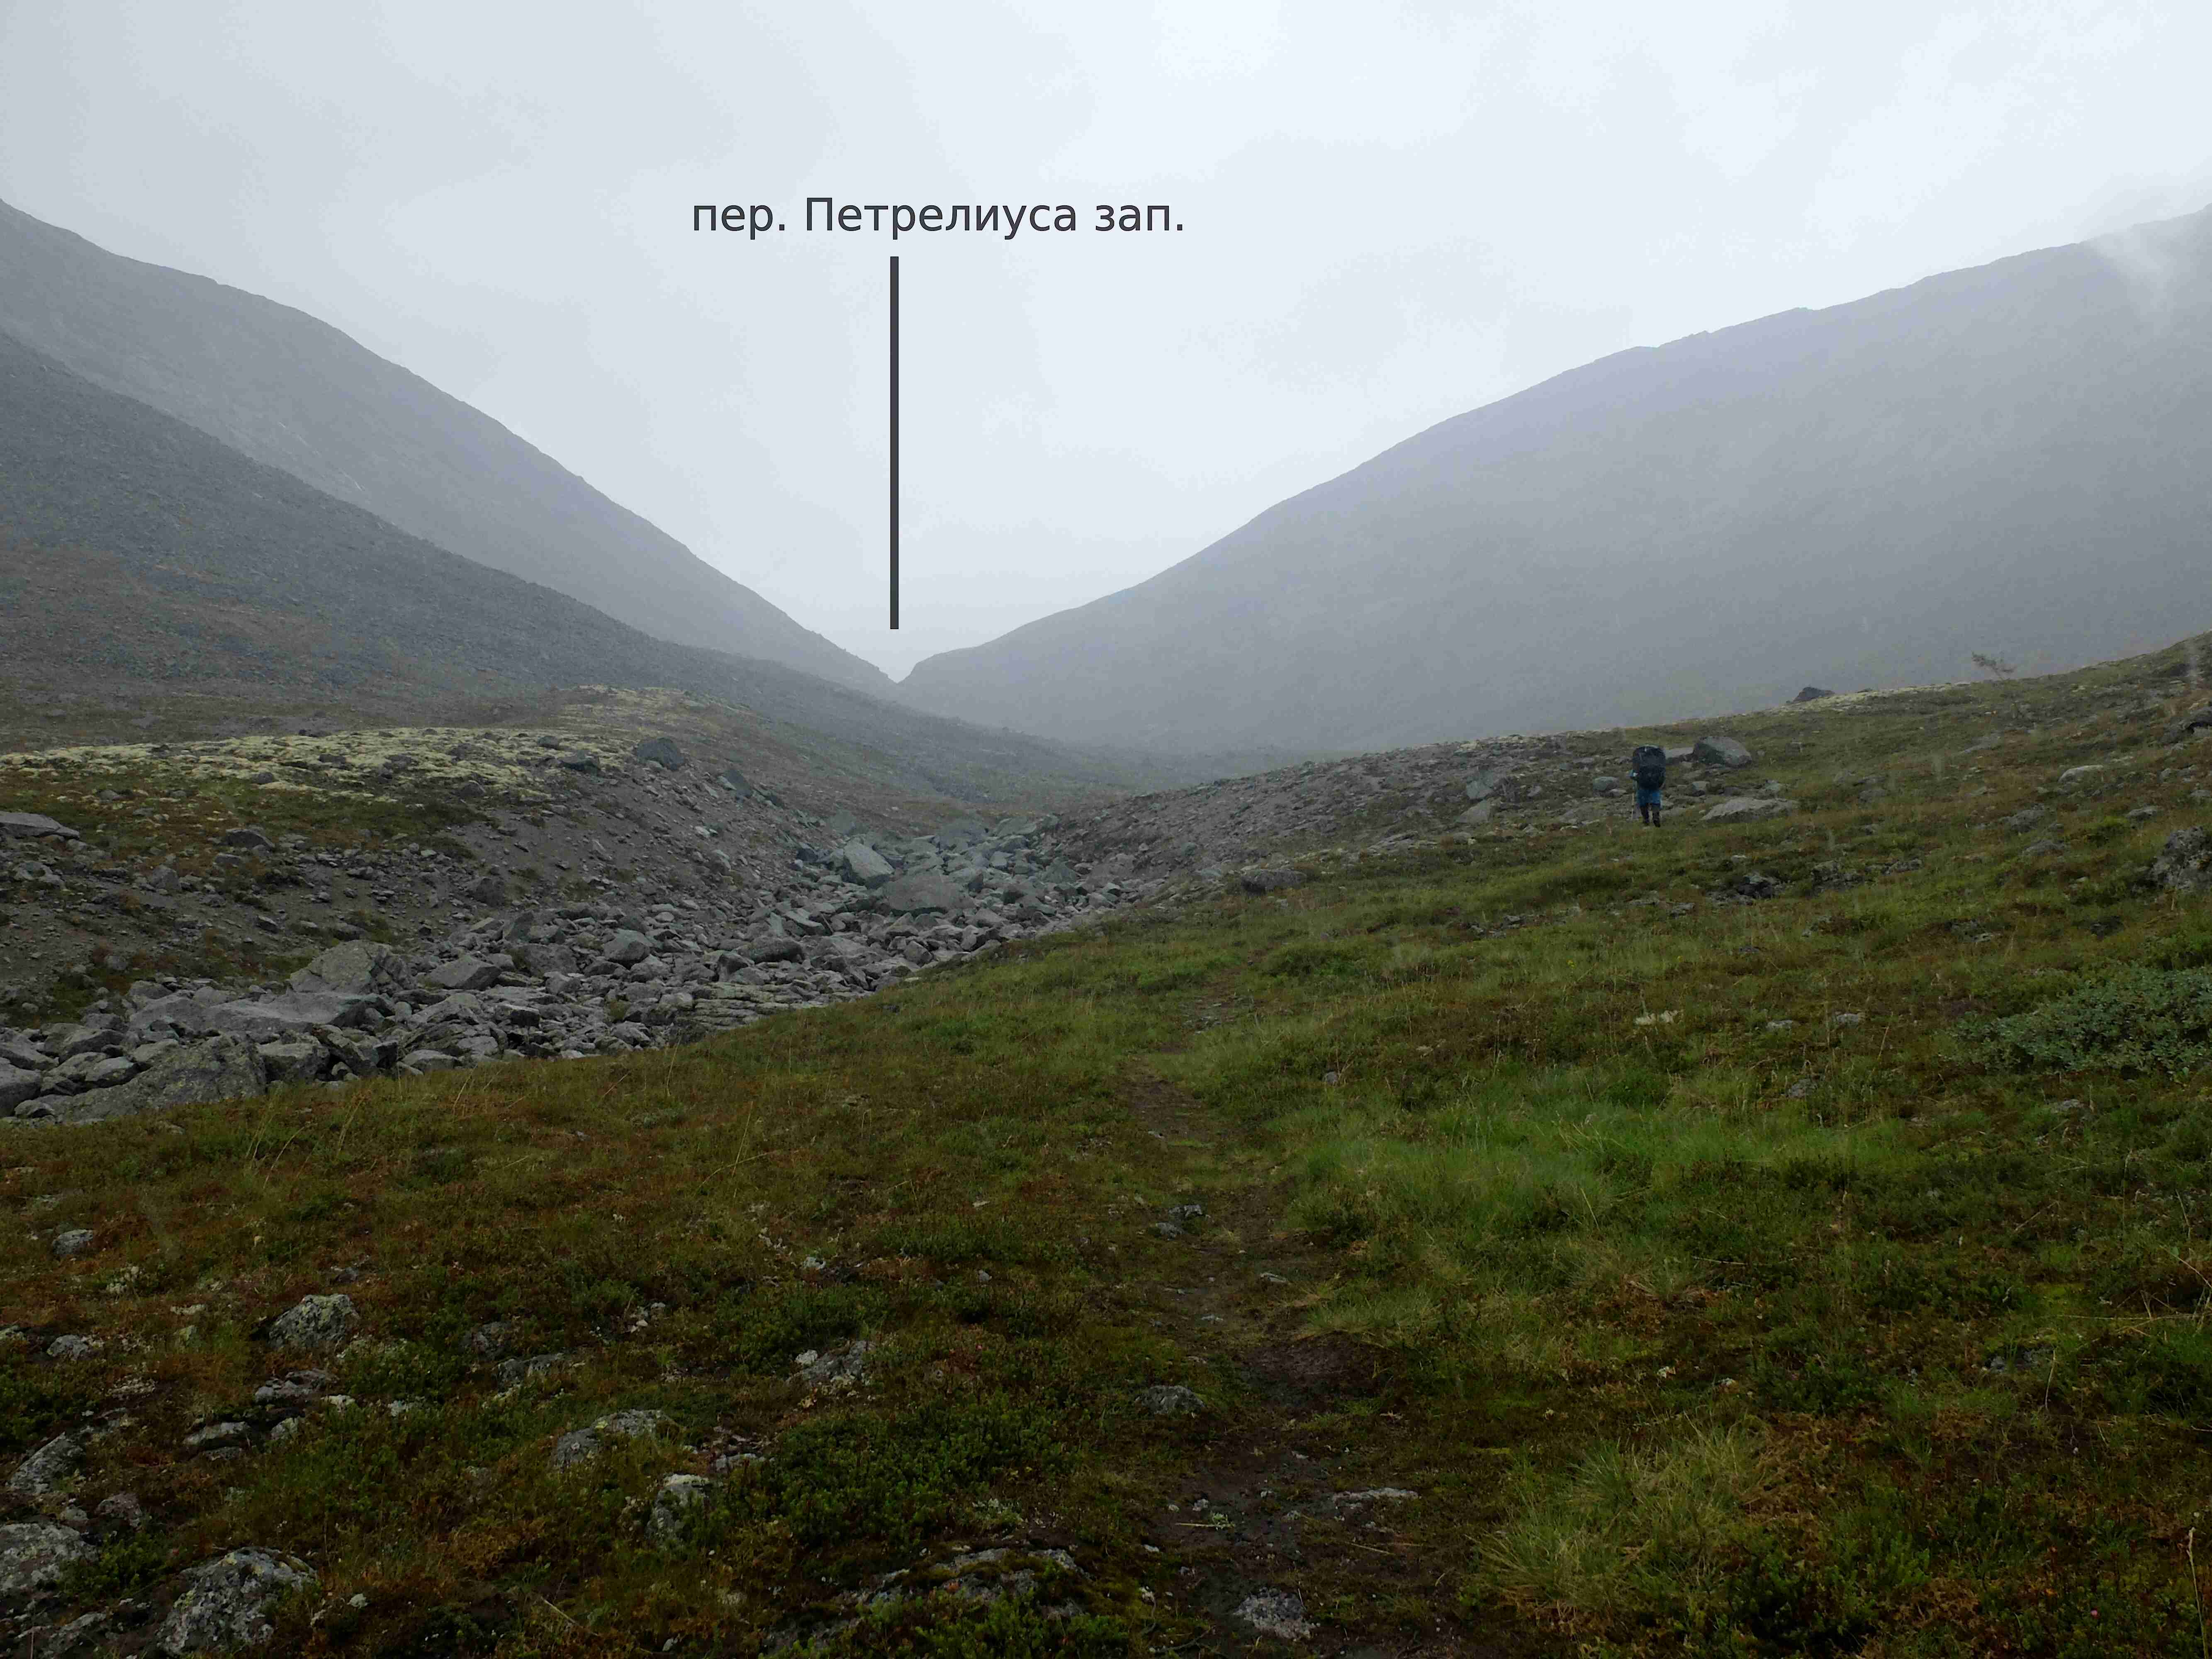
\includegraphics[width=14cm]{foto/08_08/01.Вид на перевал с юга из долины.png.jpg}
    \caption{Вид на пер. Петрелиуса Западный с юга}
    \label{fig4:1}
\end{figure}

\begin{figure}
    \centering
    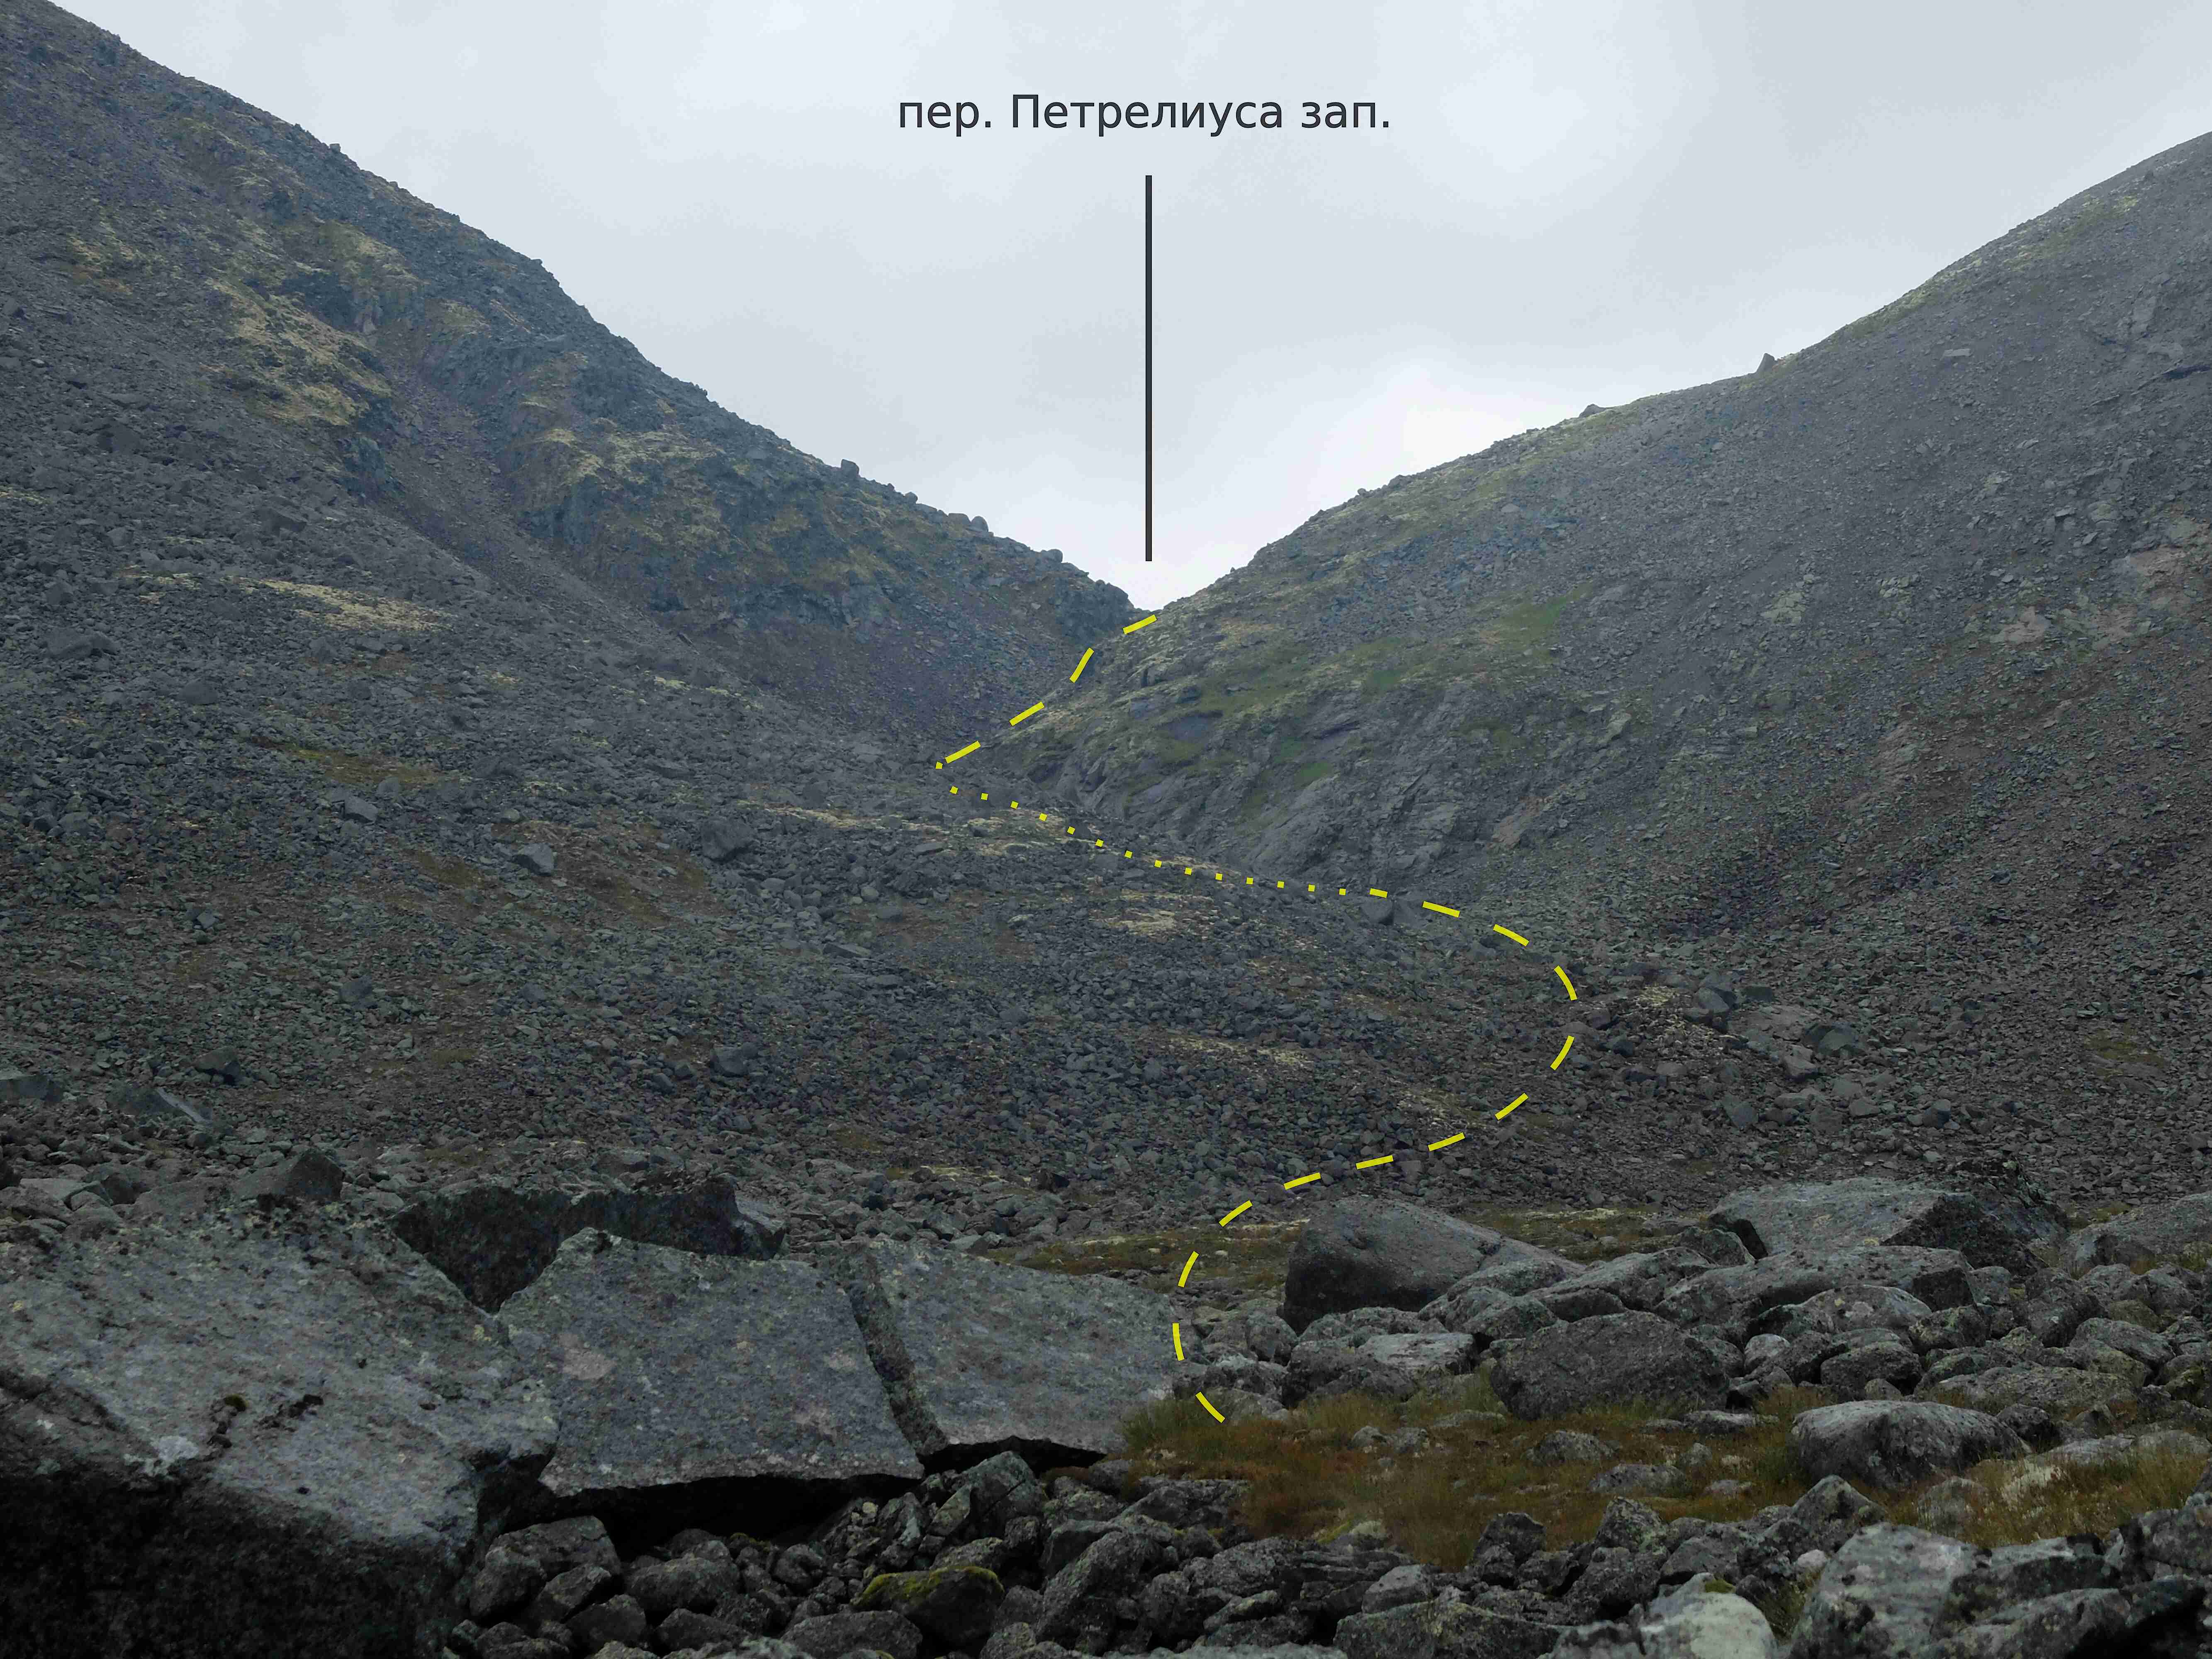
\includegraphics[width=14cm]{foto/08_08/02.Подъём на перевал.png.jpg}
    \caption{Подъём на пер. Петрелиуса Западный}
    \label{fig4:2}
\end{figure}

\begin{figure}
    \centering
    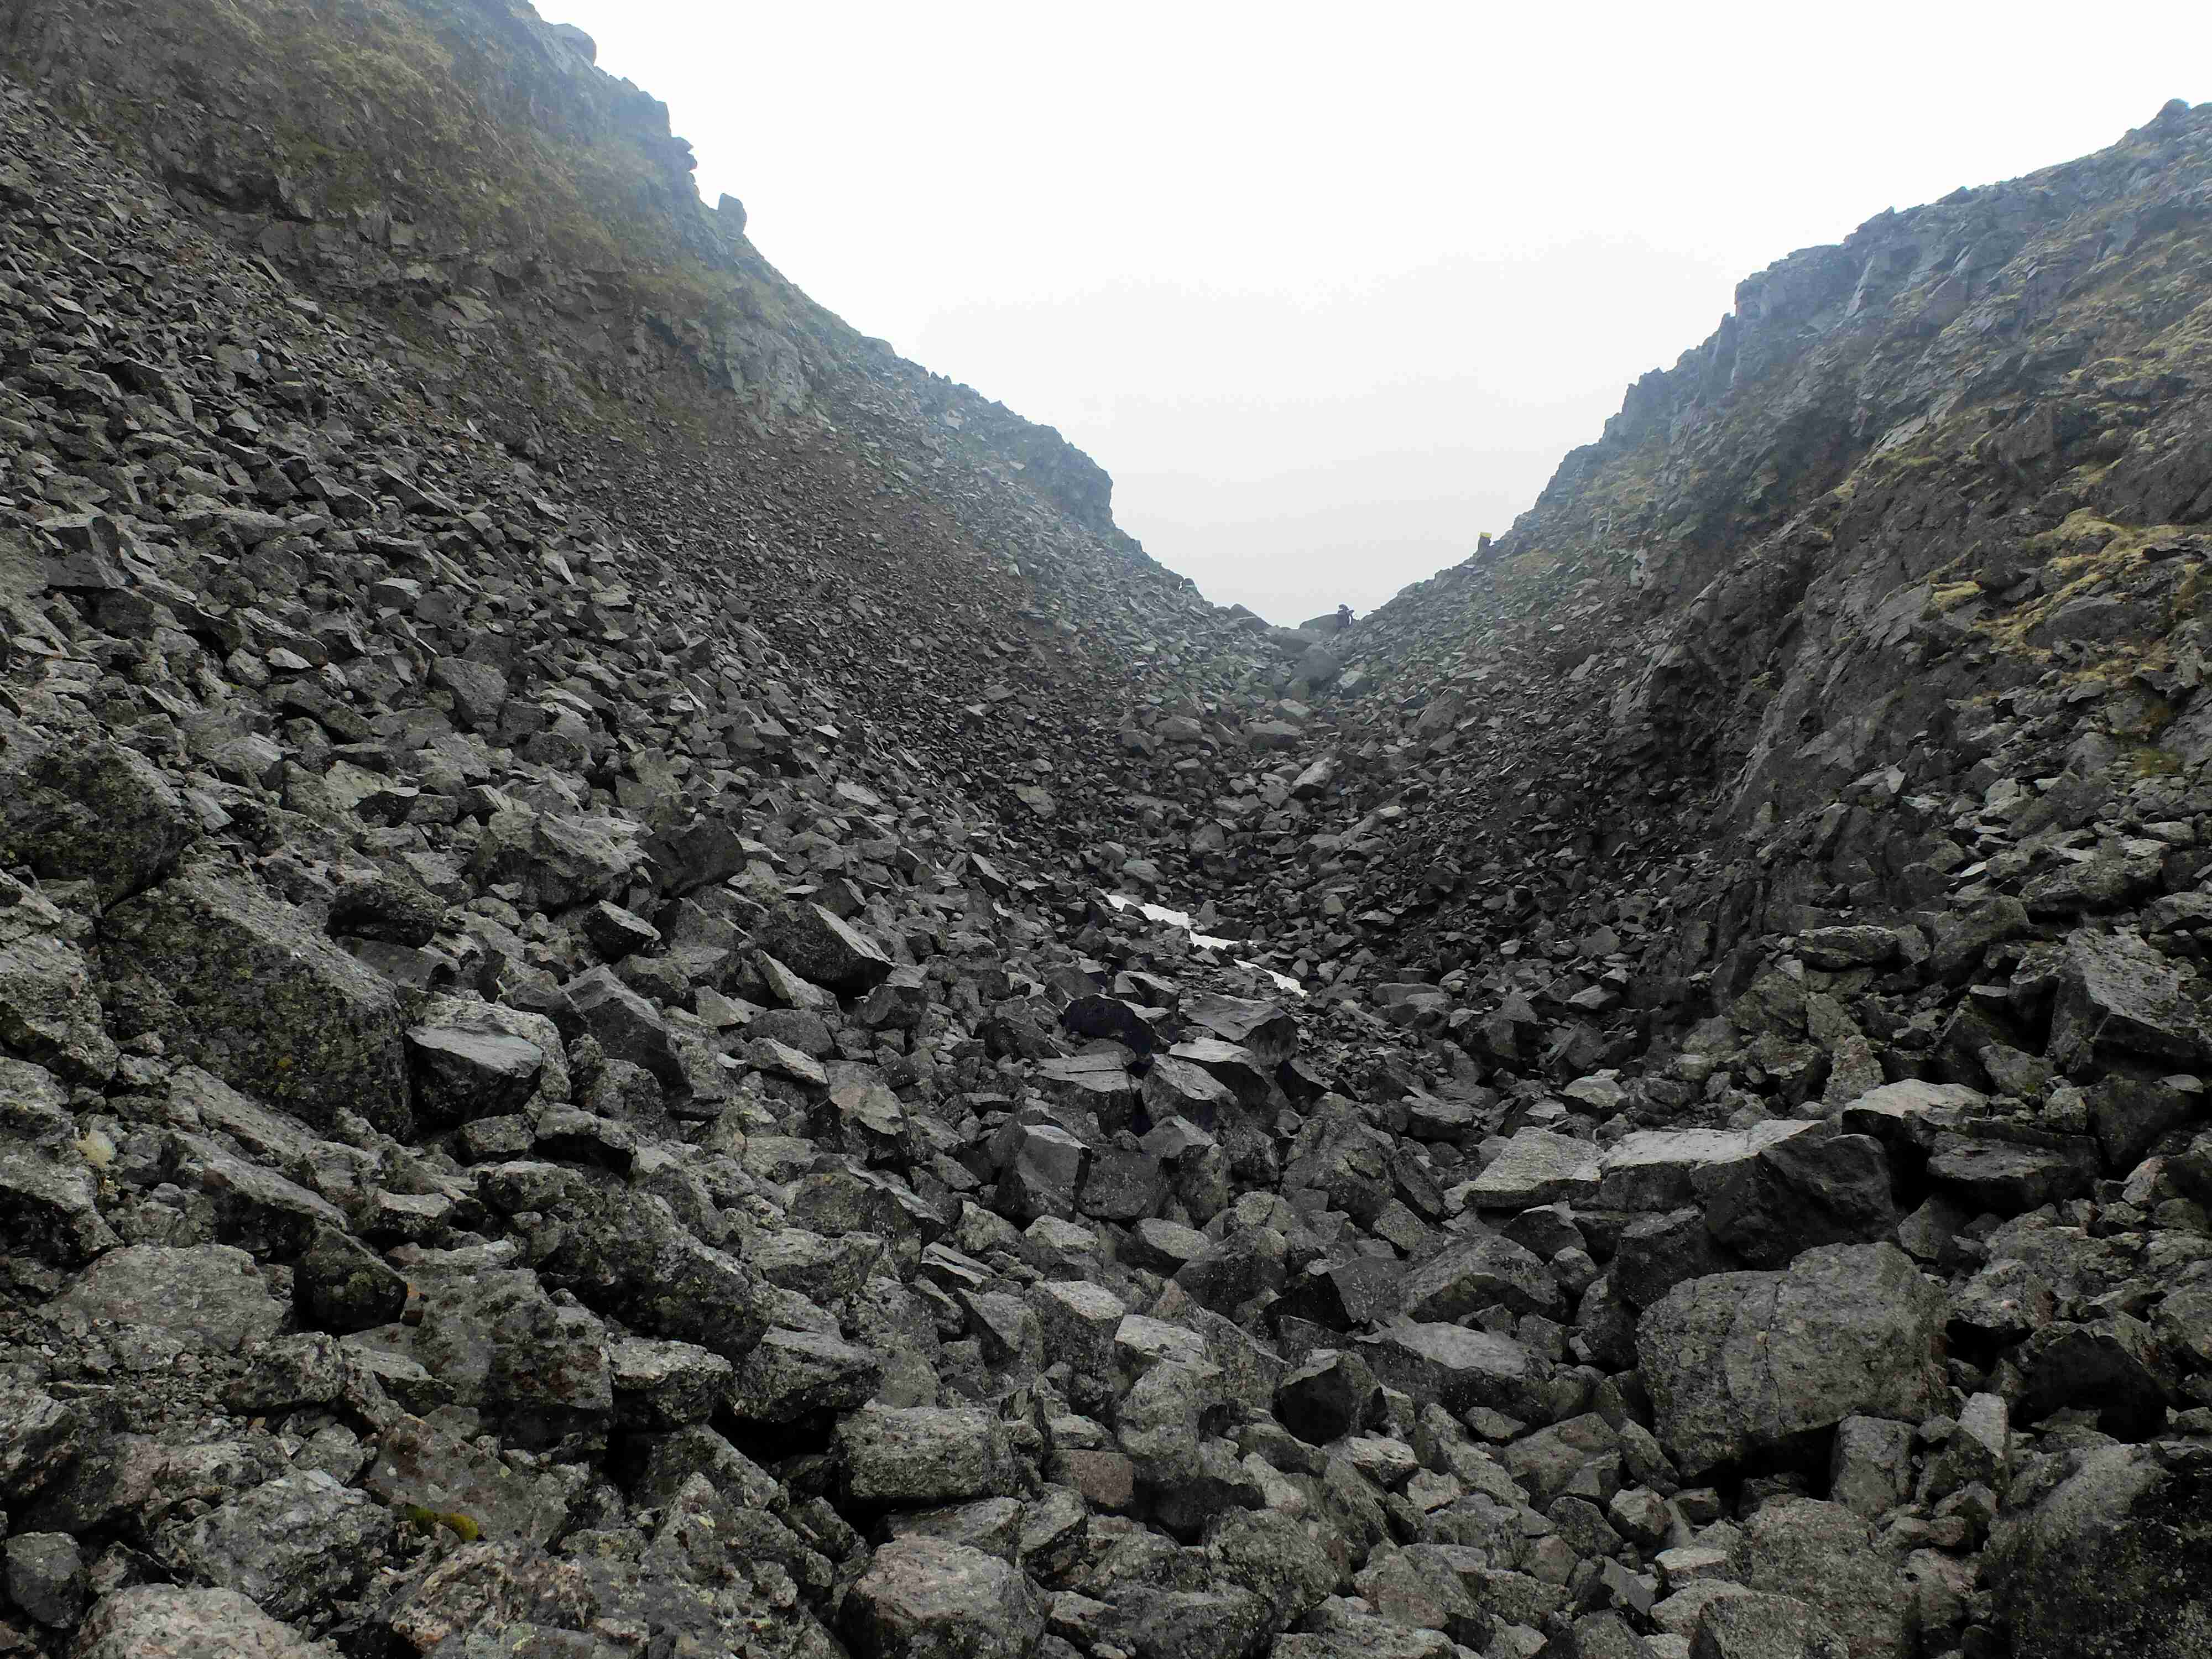
\includegraphics[width=14cm]{foto/08_08/03.Перевальный взлет.png.jpg}
    \caption{Перевальный взлёт}
    \label{fig4:3}
\end{figure}

\begin{figure}
    \centering
    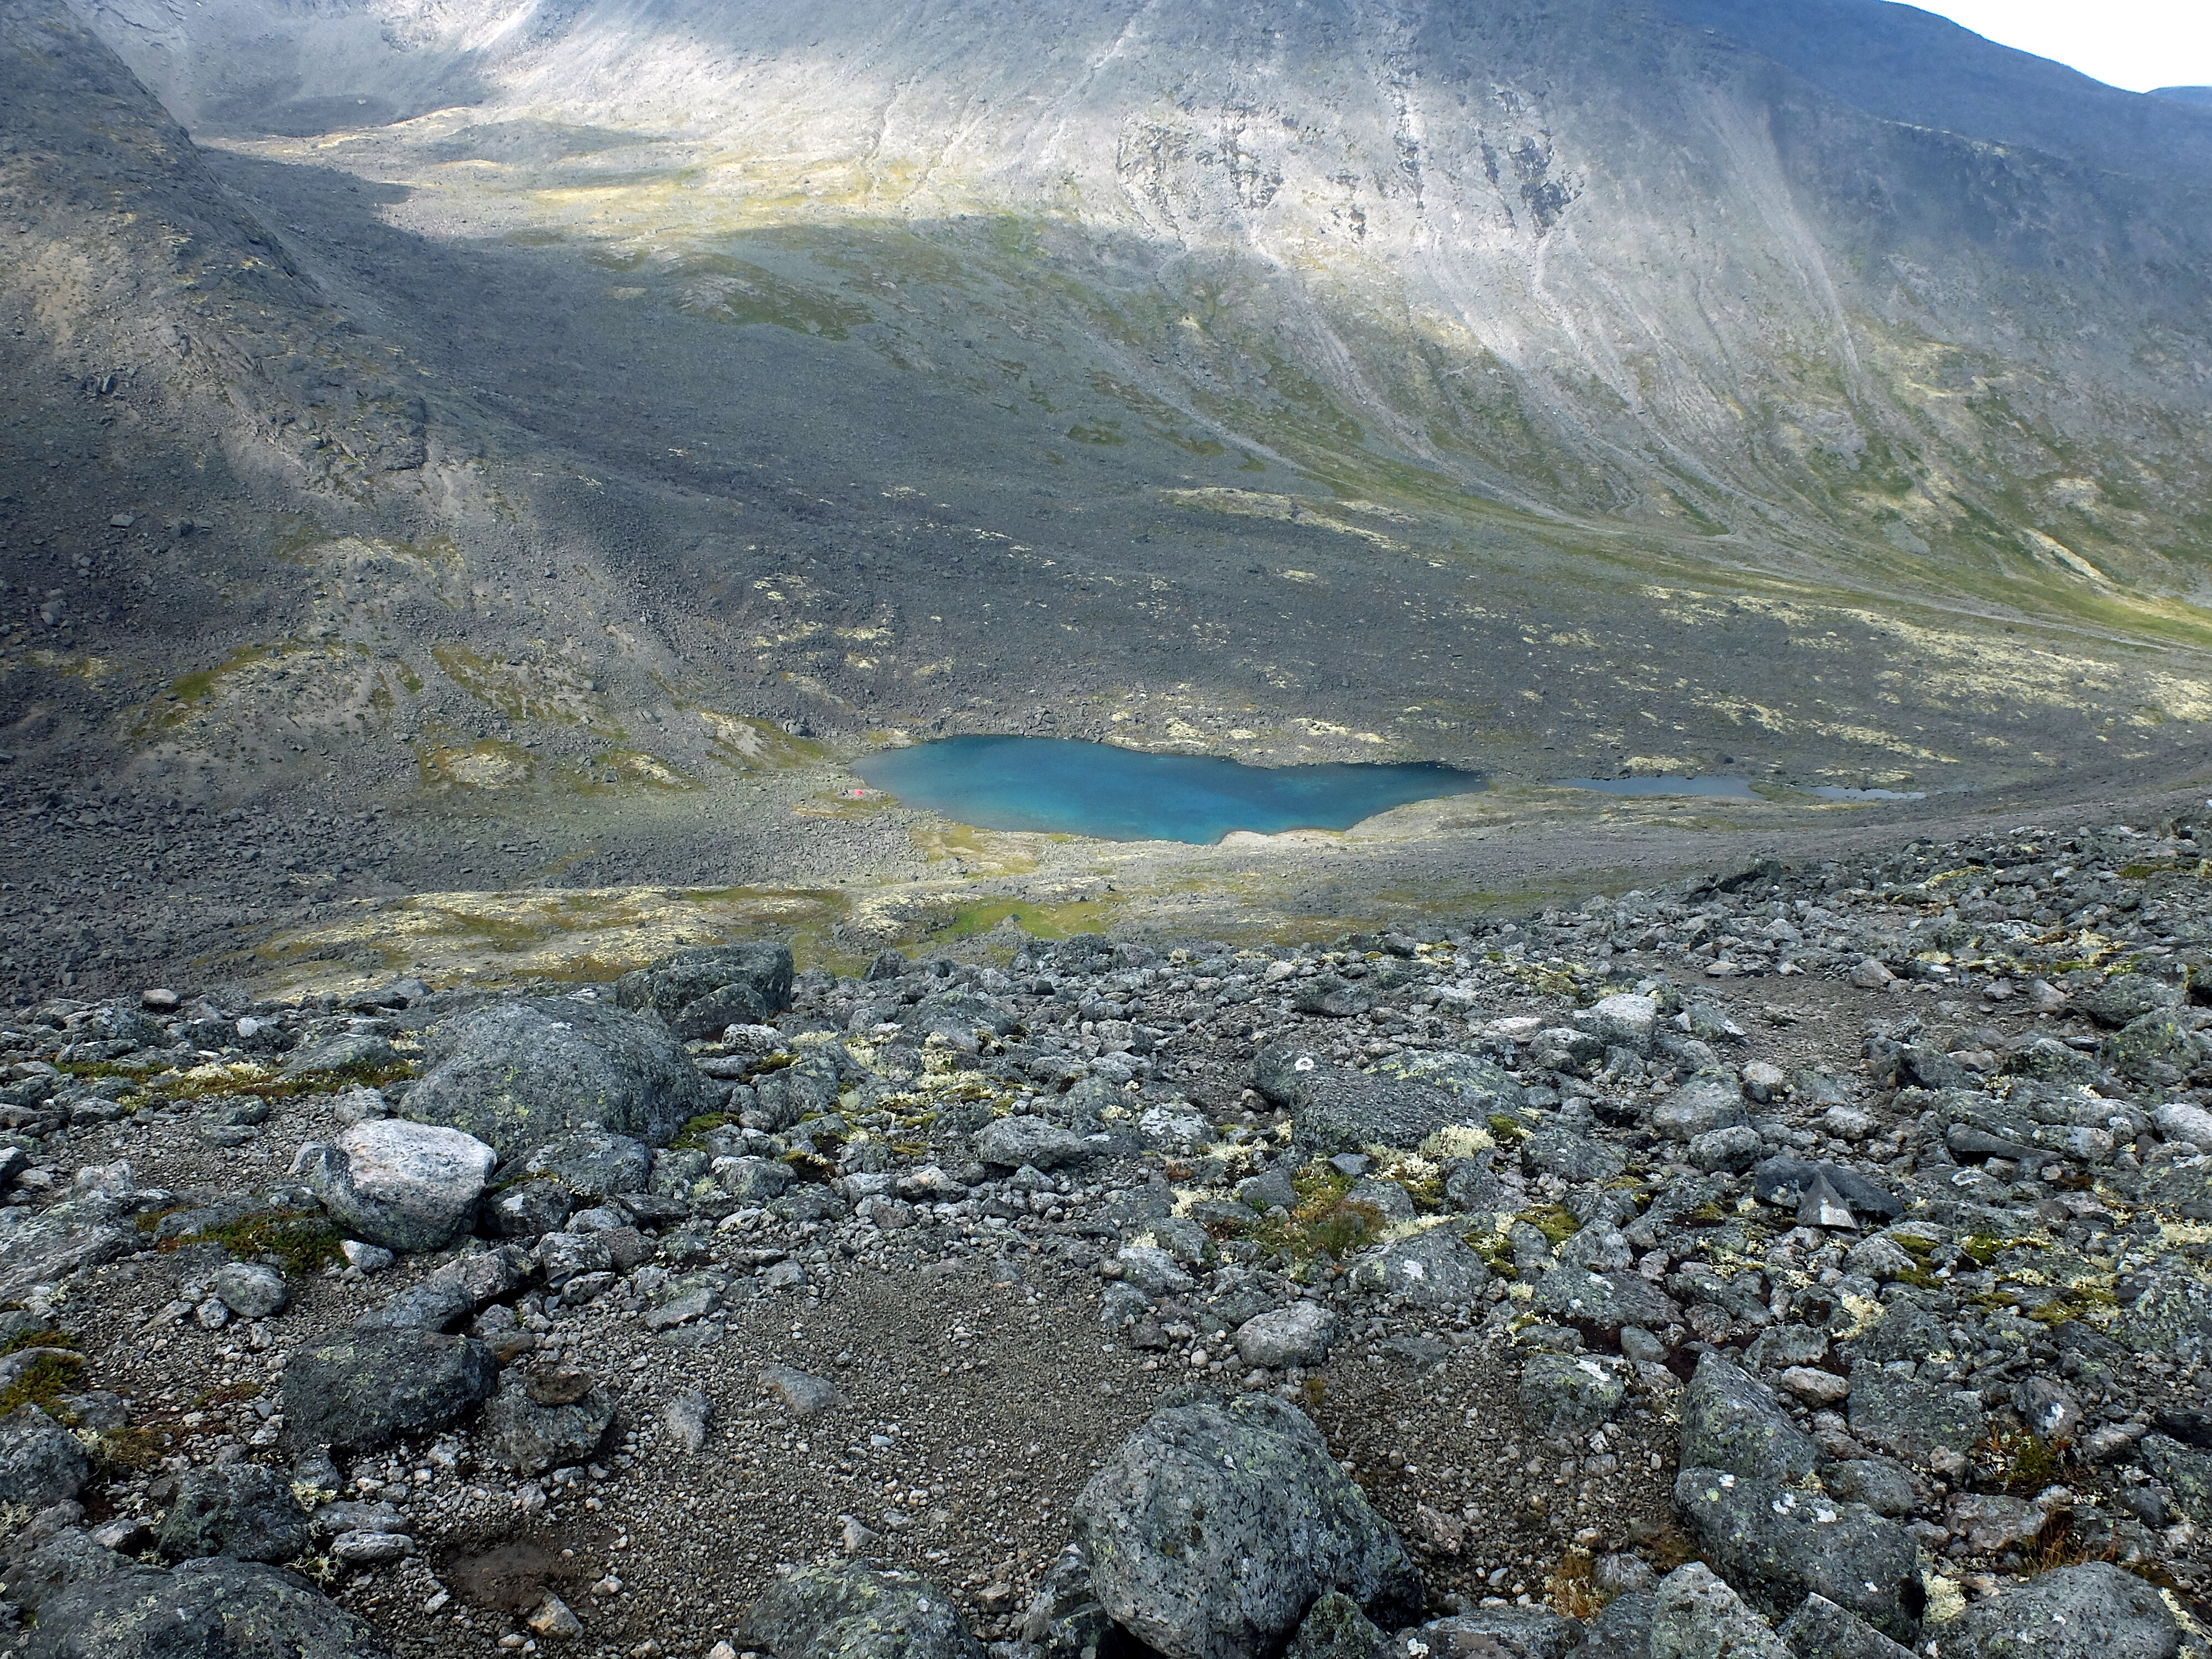
\includegraphics[width=14cm]{foto/08_08/04.Спуск с перевала в долину.png.jpg}
    \caption{Вид с пер. Петрелиуса Западный в долину руч. Петрелиуса}
    \label{fig4:4}
\end{figure}

\begin{figure}
    \centering
    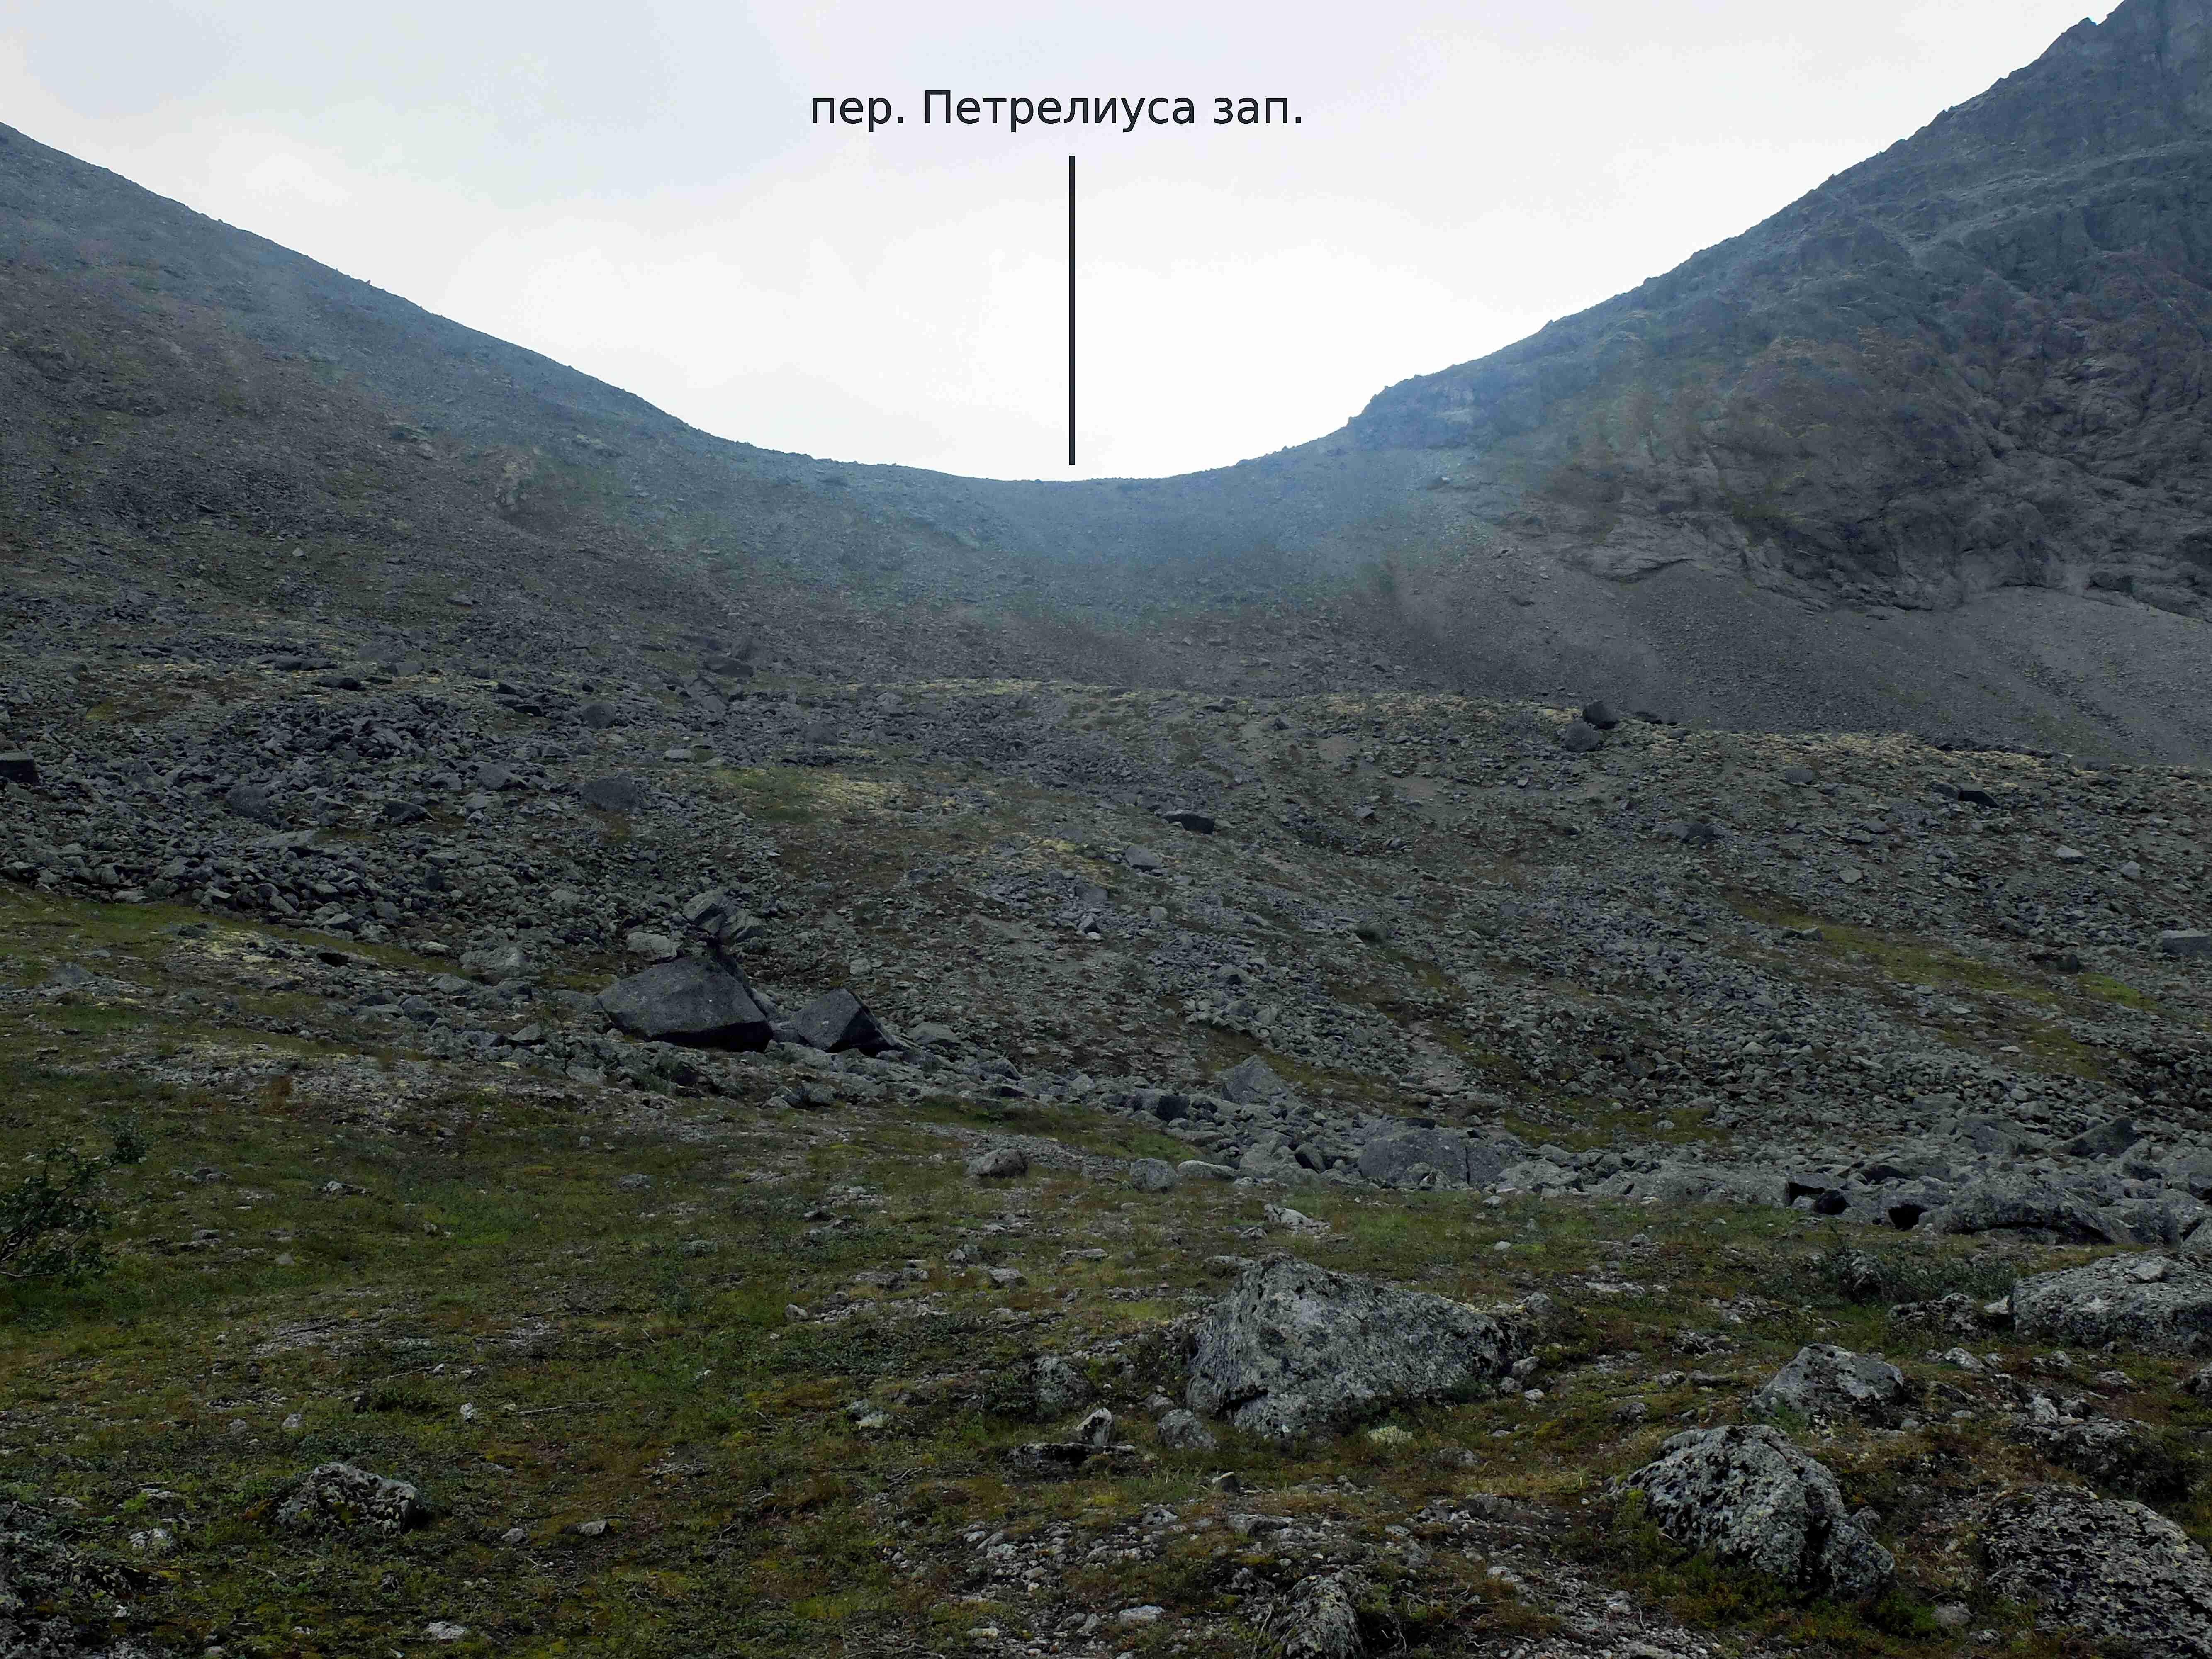
\includegraphics[width=14cm]{foto/08_08/05.Подъём на перевал от озера с севера.png.jpg}
    \caption{Подъём на пер. Петрелиуса Западный с севера}
    \label{fig4:5}
\end{figure}

\begin{figure}
    \centering
    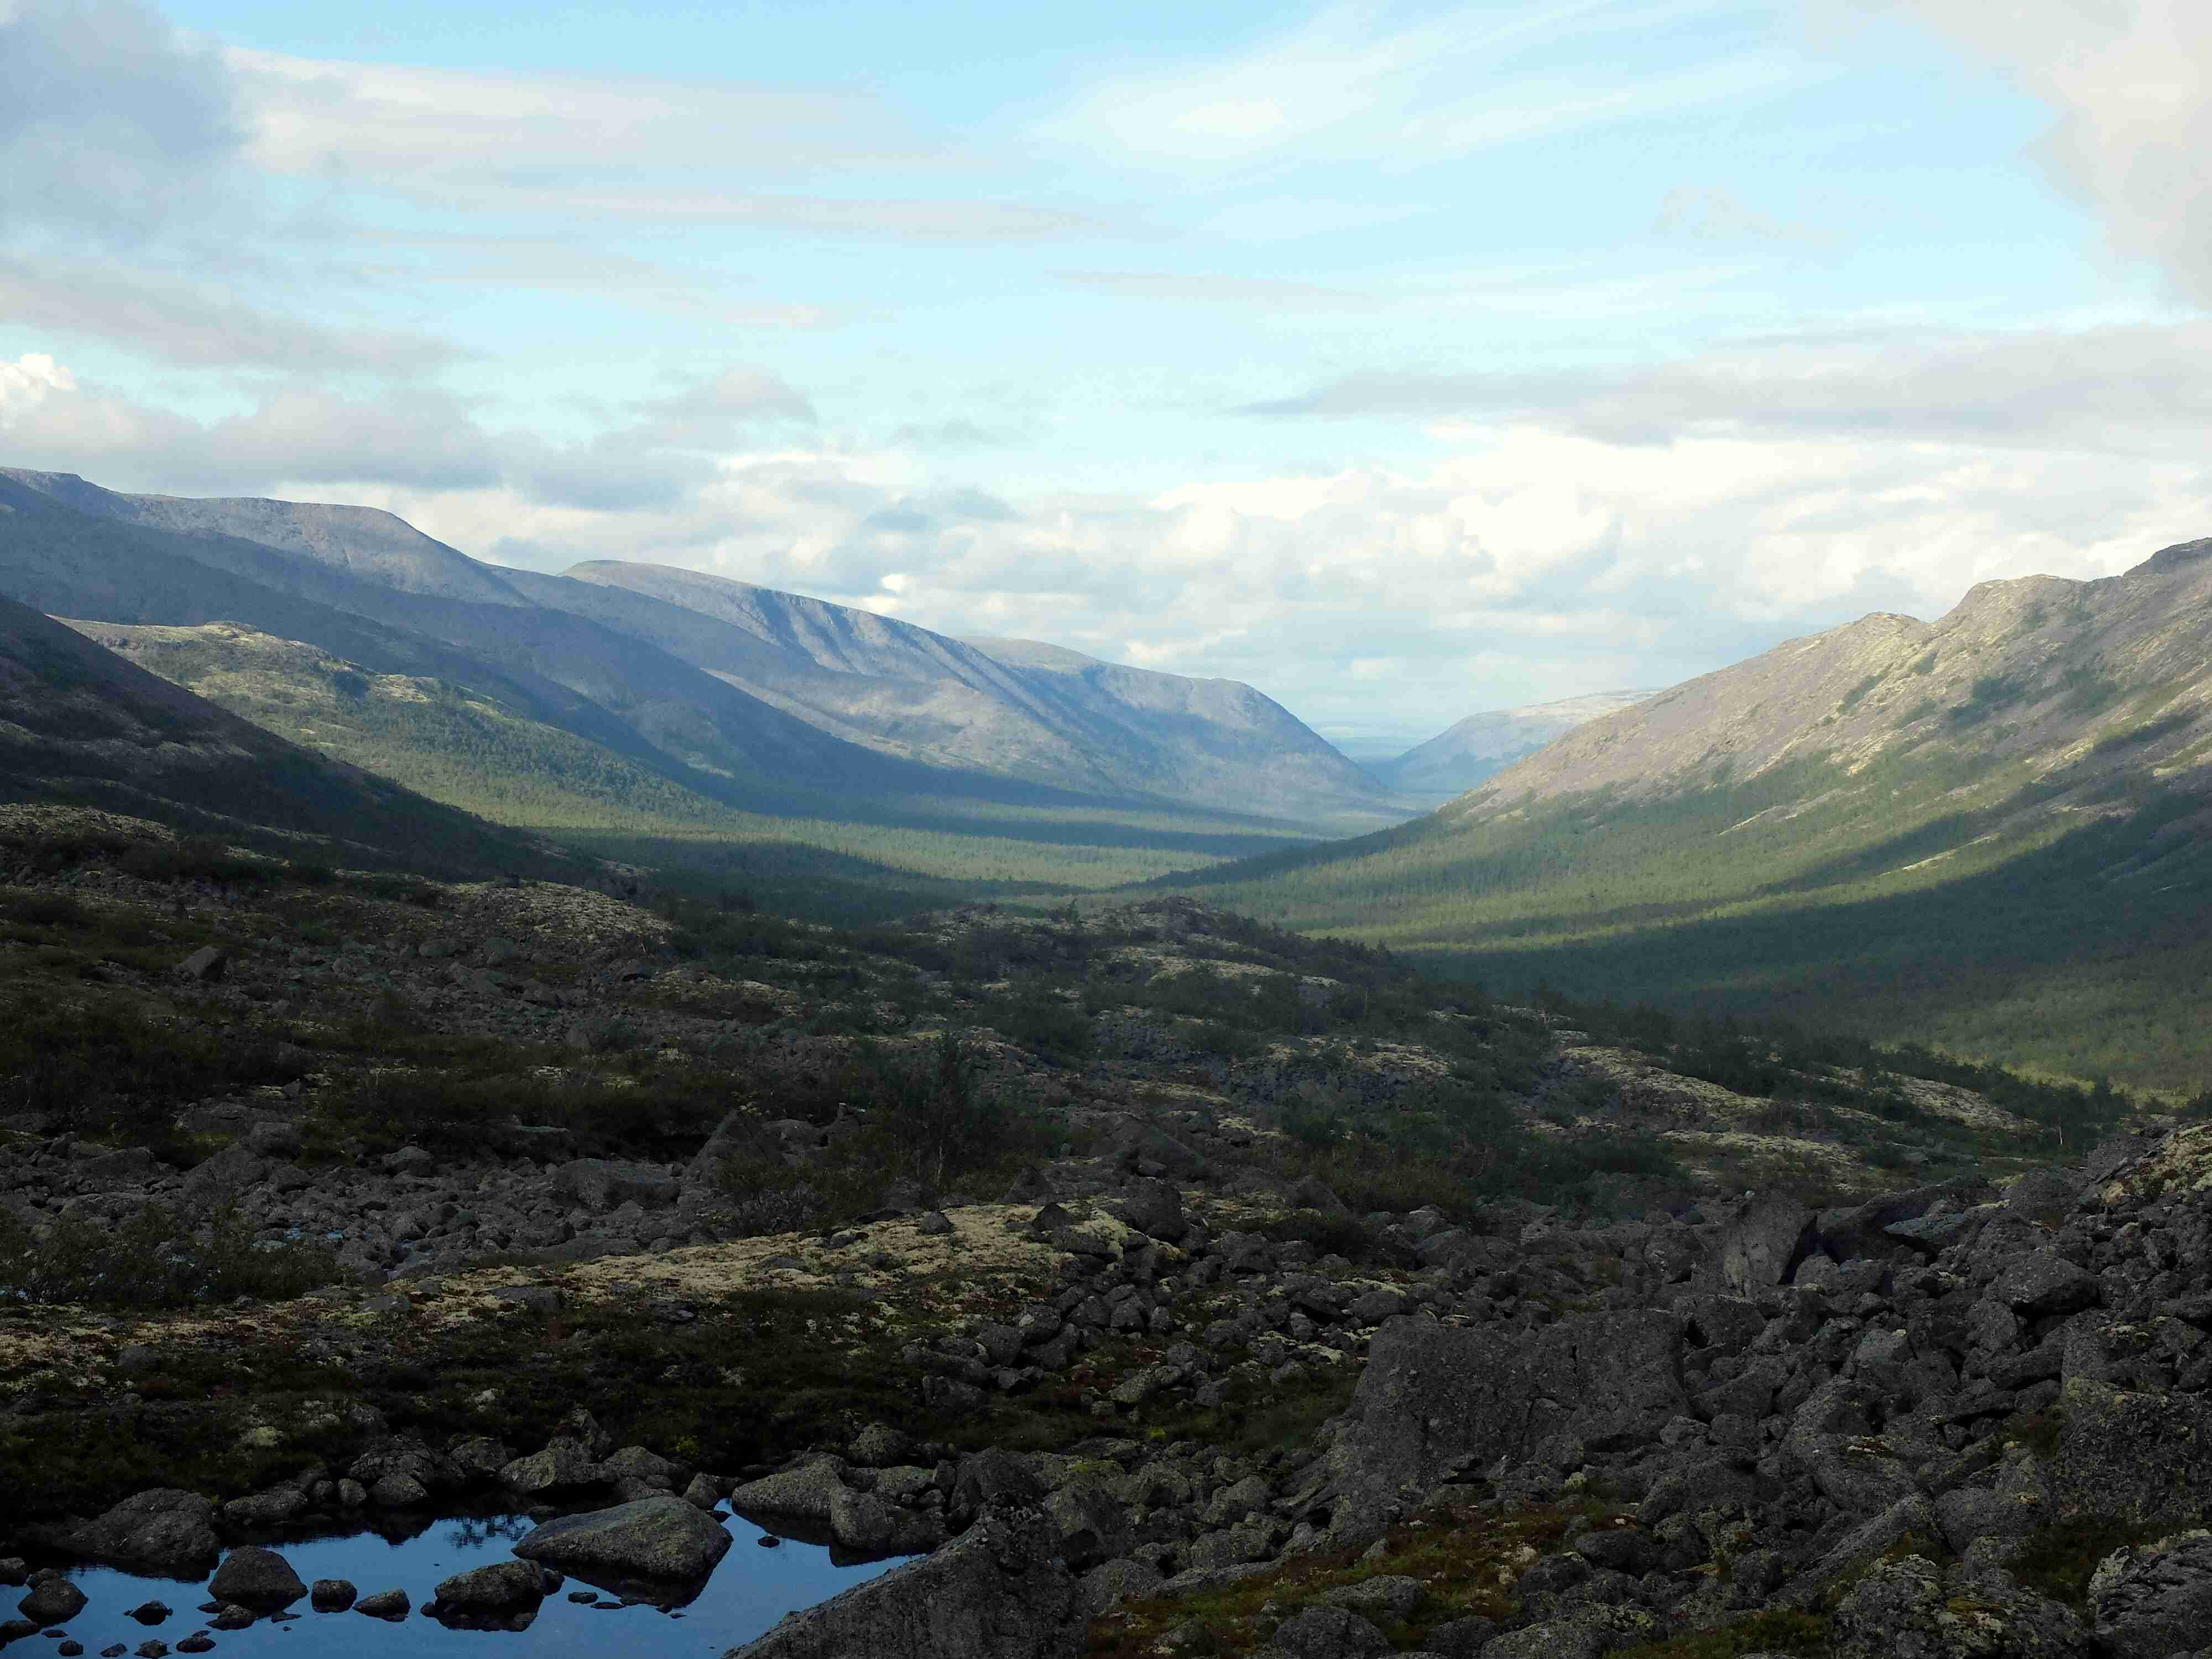
\includegraphics[width=14cm]{foto/08_08/06.Долина от перевала.png.jpg}
    \caption{Долина руч. Петрелиуса}
    \label{fig4:6}
\end{figure}

\begin{figure}
    \centering
    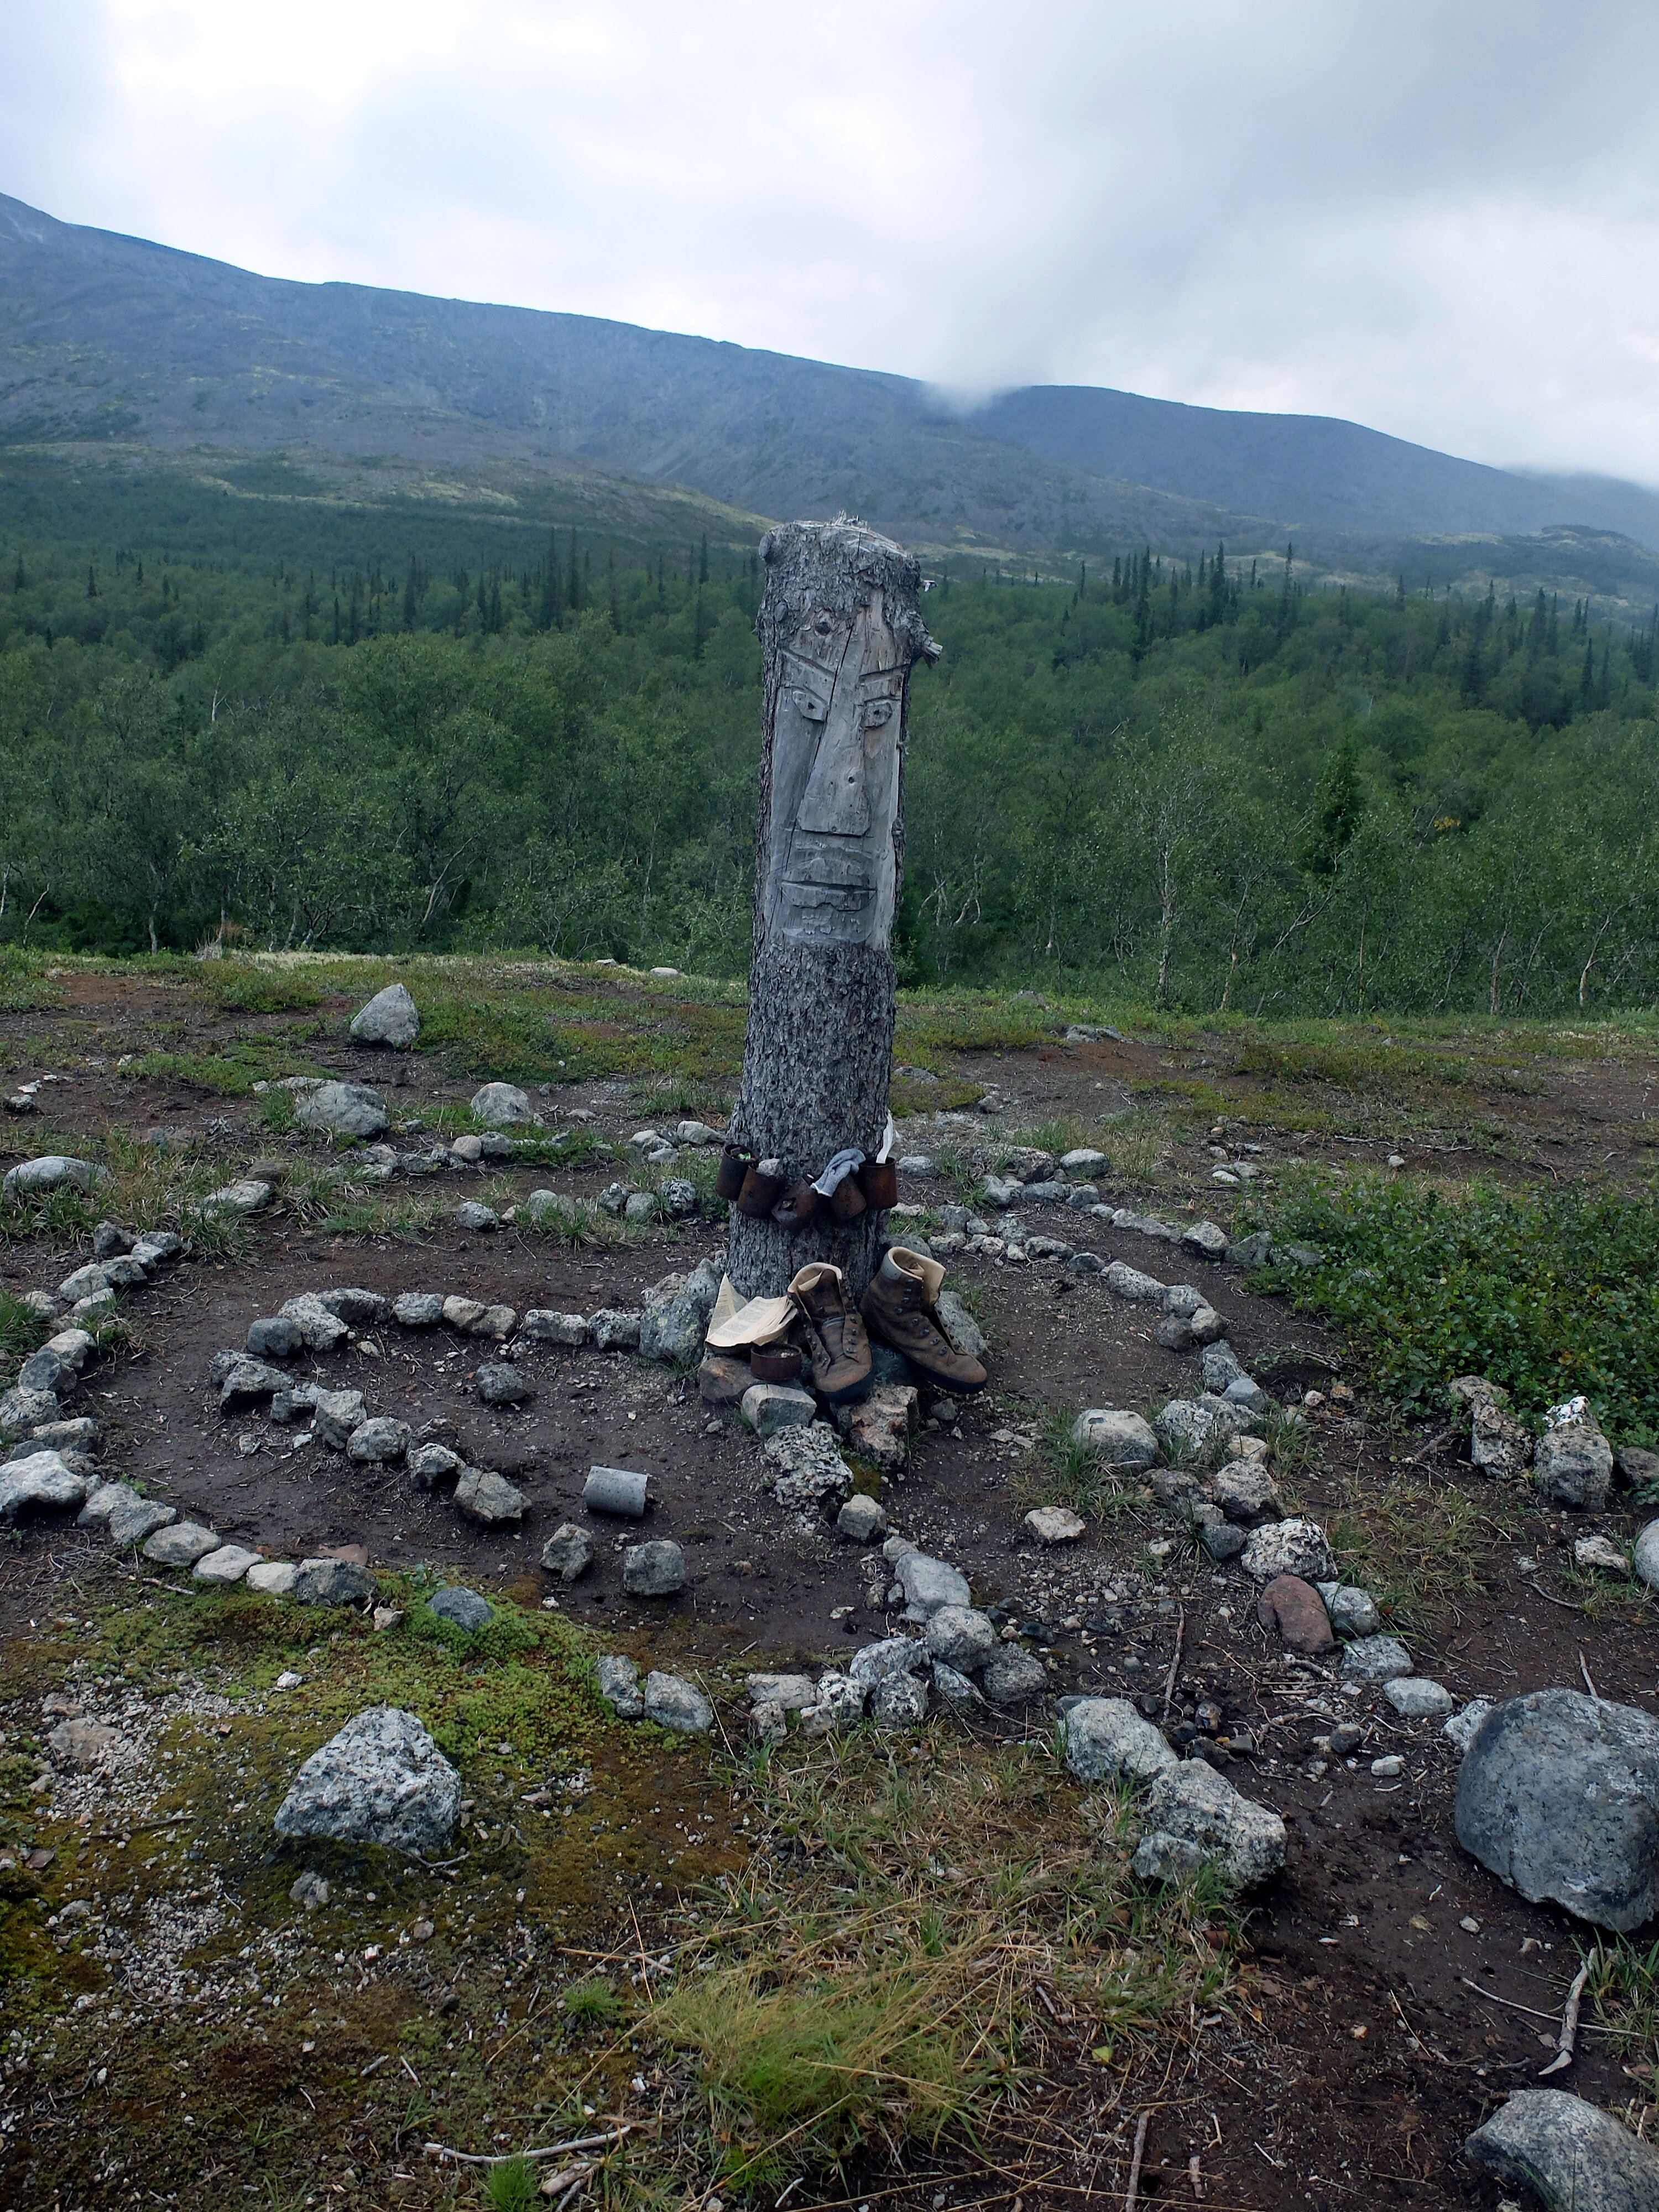
\includegraphics[width=8cm]{foto/08_08/07.Истукан на стоянке.png.jpg}
    \caption{Истукан на стоянке}
    \label{fig4:7}
\end{figure}

\FloatBarrier

\subsection{День 5. 09.08.2022\\
Руч. Петрелиуса -- р. Кунийок -- оз. Гольцовое  -- руч. Партомйок -- пер. Умбозёрский (н/к, 527 м) -- р. Северный Каскаснюнйок}
\begin{tabular}{l p{12cm}}
\hline
Пройдено: & 18.28 км\\
Набор/сброс высоты: & 632/515 м\\
Время в пути: & 8:44\\
ЧХВ: & 5:44\\
Метеоусловия: & Первая половина дня --- ясно. Вторая --- пасмурно, без дождя.\\
\hline
\end{tabular}

08:10 Подъём. Переменная облачность, +15$\tccentigrade$.

10:27 Выходим.
Тут же солнце вышло из облаков и было солнечно до нашего обеда.
На карте, ниже по течению руч. Петрелиуса, через 600 метров нарисован автоброд.
У самого автоброда стоит указатель “мост” и стрелка вниз по течению, и действительно --- метров через 50 вдоль берега
вниз по течению есть пешеходный мостик (рис. \ref{fig5:1}). Судя по разбросанным деревянным паллетам выше и ниже автоброда и
моста, здесь либо потерпел аварию грузовик с паллетами, либо же пешеходный мост регулярно сносит течением.

10:41 Переходим на левый берег. Далее идём проезжей дороге около 3.5 километра до моста,
который расположен сразу за КСС “Куэльпорр”. Здесь уже руч. Петрелиуса влился в р. Кунийок.

12:01 База КСС. Регистрируемся в МЧС, рассматриваем тамошние достопримечательности.
Сотрудник МЧС сообщает, что нас ищут с полицией. Ну что поделаешь --- горы.

12:27 Отправляемся по автомобильной дороге до оз. Гольцового. Леса нет --- лес сгорел.
Справа ответвление на пер. Умбозёрский. Встречаем автотуриста, ходившего с собаками в радиалку на Умбозёрский.
Ближе к оз. Щучьему начинается лес, разливы по дорогам. Сквозь деревья видно несколько групп отдыхающих, с автомобилями.
К Гольцовому подходим заболоченными рыбачьими тропами.

13:58 Полянка у впадения Кунийока в Гольцовое (рис. \ref{fig5:2}). Солнце прячется, дальше пасмурно до конца дня,
но без дождя, +20$\tccentigrade$.
Становимся на обед. Вид на север, уже за пределы Хибин, а на первом плане озеро с рыбаками,
бродящими вблизи берега в сапогах. Связь эпизодическая, одна палочка на вытянутой руке. Пытаемся связаться,
sms кое-как отправились (успешно, как потом оказалось), от обратных пришло только уведомление, текст не принялся.

15:43 Выдвигаемся на пер. Умбозёрский. После отворота с дороги на КСС --- вездеходная дорога через лес.
Пару раз навстречу проезжают внедорожники. Дорога несколько раз переходит с одной стороны руч. Партомйок на другую
(рис. \ref{fig5:3}),
и нам приходится переходить ручей вброд вслед за ней. Лес постепенно переходит в кустарник (рис. \ref{fig5:4}),
потом и тот исчезает.
Обходим безымянное озеро, большая группа молодёжи спускается навстречу в сторону КСС, наверное студенты.

18:03 Перевал. Снимаем пару записок: 1) группы туристов т/к \enquote{Белая гора} под рук. Каплана Л.В. от 05.08.2022;
2) группы туристов из г. Новоур(альска?) под рук. Мариевского Дмитрия от 30.07.2022 (рис. \ref{fig:zapiski3}).
Попытались забраться повыше, чтобы поймать сотовую связь (благо пологие стенки перевала это позволяли), но не преуспели.

18:27 Идём дальше (рис. \ref{fig5:5}--\ref{fig5:6}). Сразу за перевалом ещё озеро, очень ветренно. Навстречу большая группа
с рюкзаками.  Примерно через 1 километр ещё одно озеро. Решаем остановиться там на ночлег 19:11.
Расчищенных площадок нет, поэтому выбираем место поровнее и ставимся на мох у берега на открытом месте.
Пока ужинаем крепчает ветер, приходится усилить палатку оттяжками и надеяться, что ночью не унесёт.

23:15 Отбой.

\begin{figure}
    \centering
    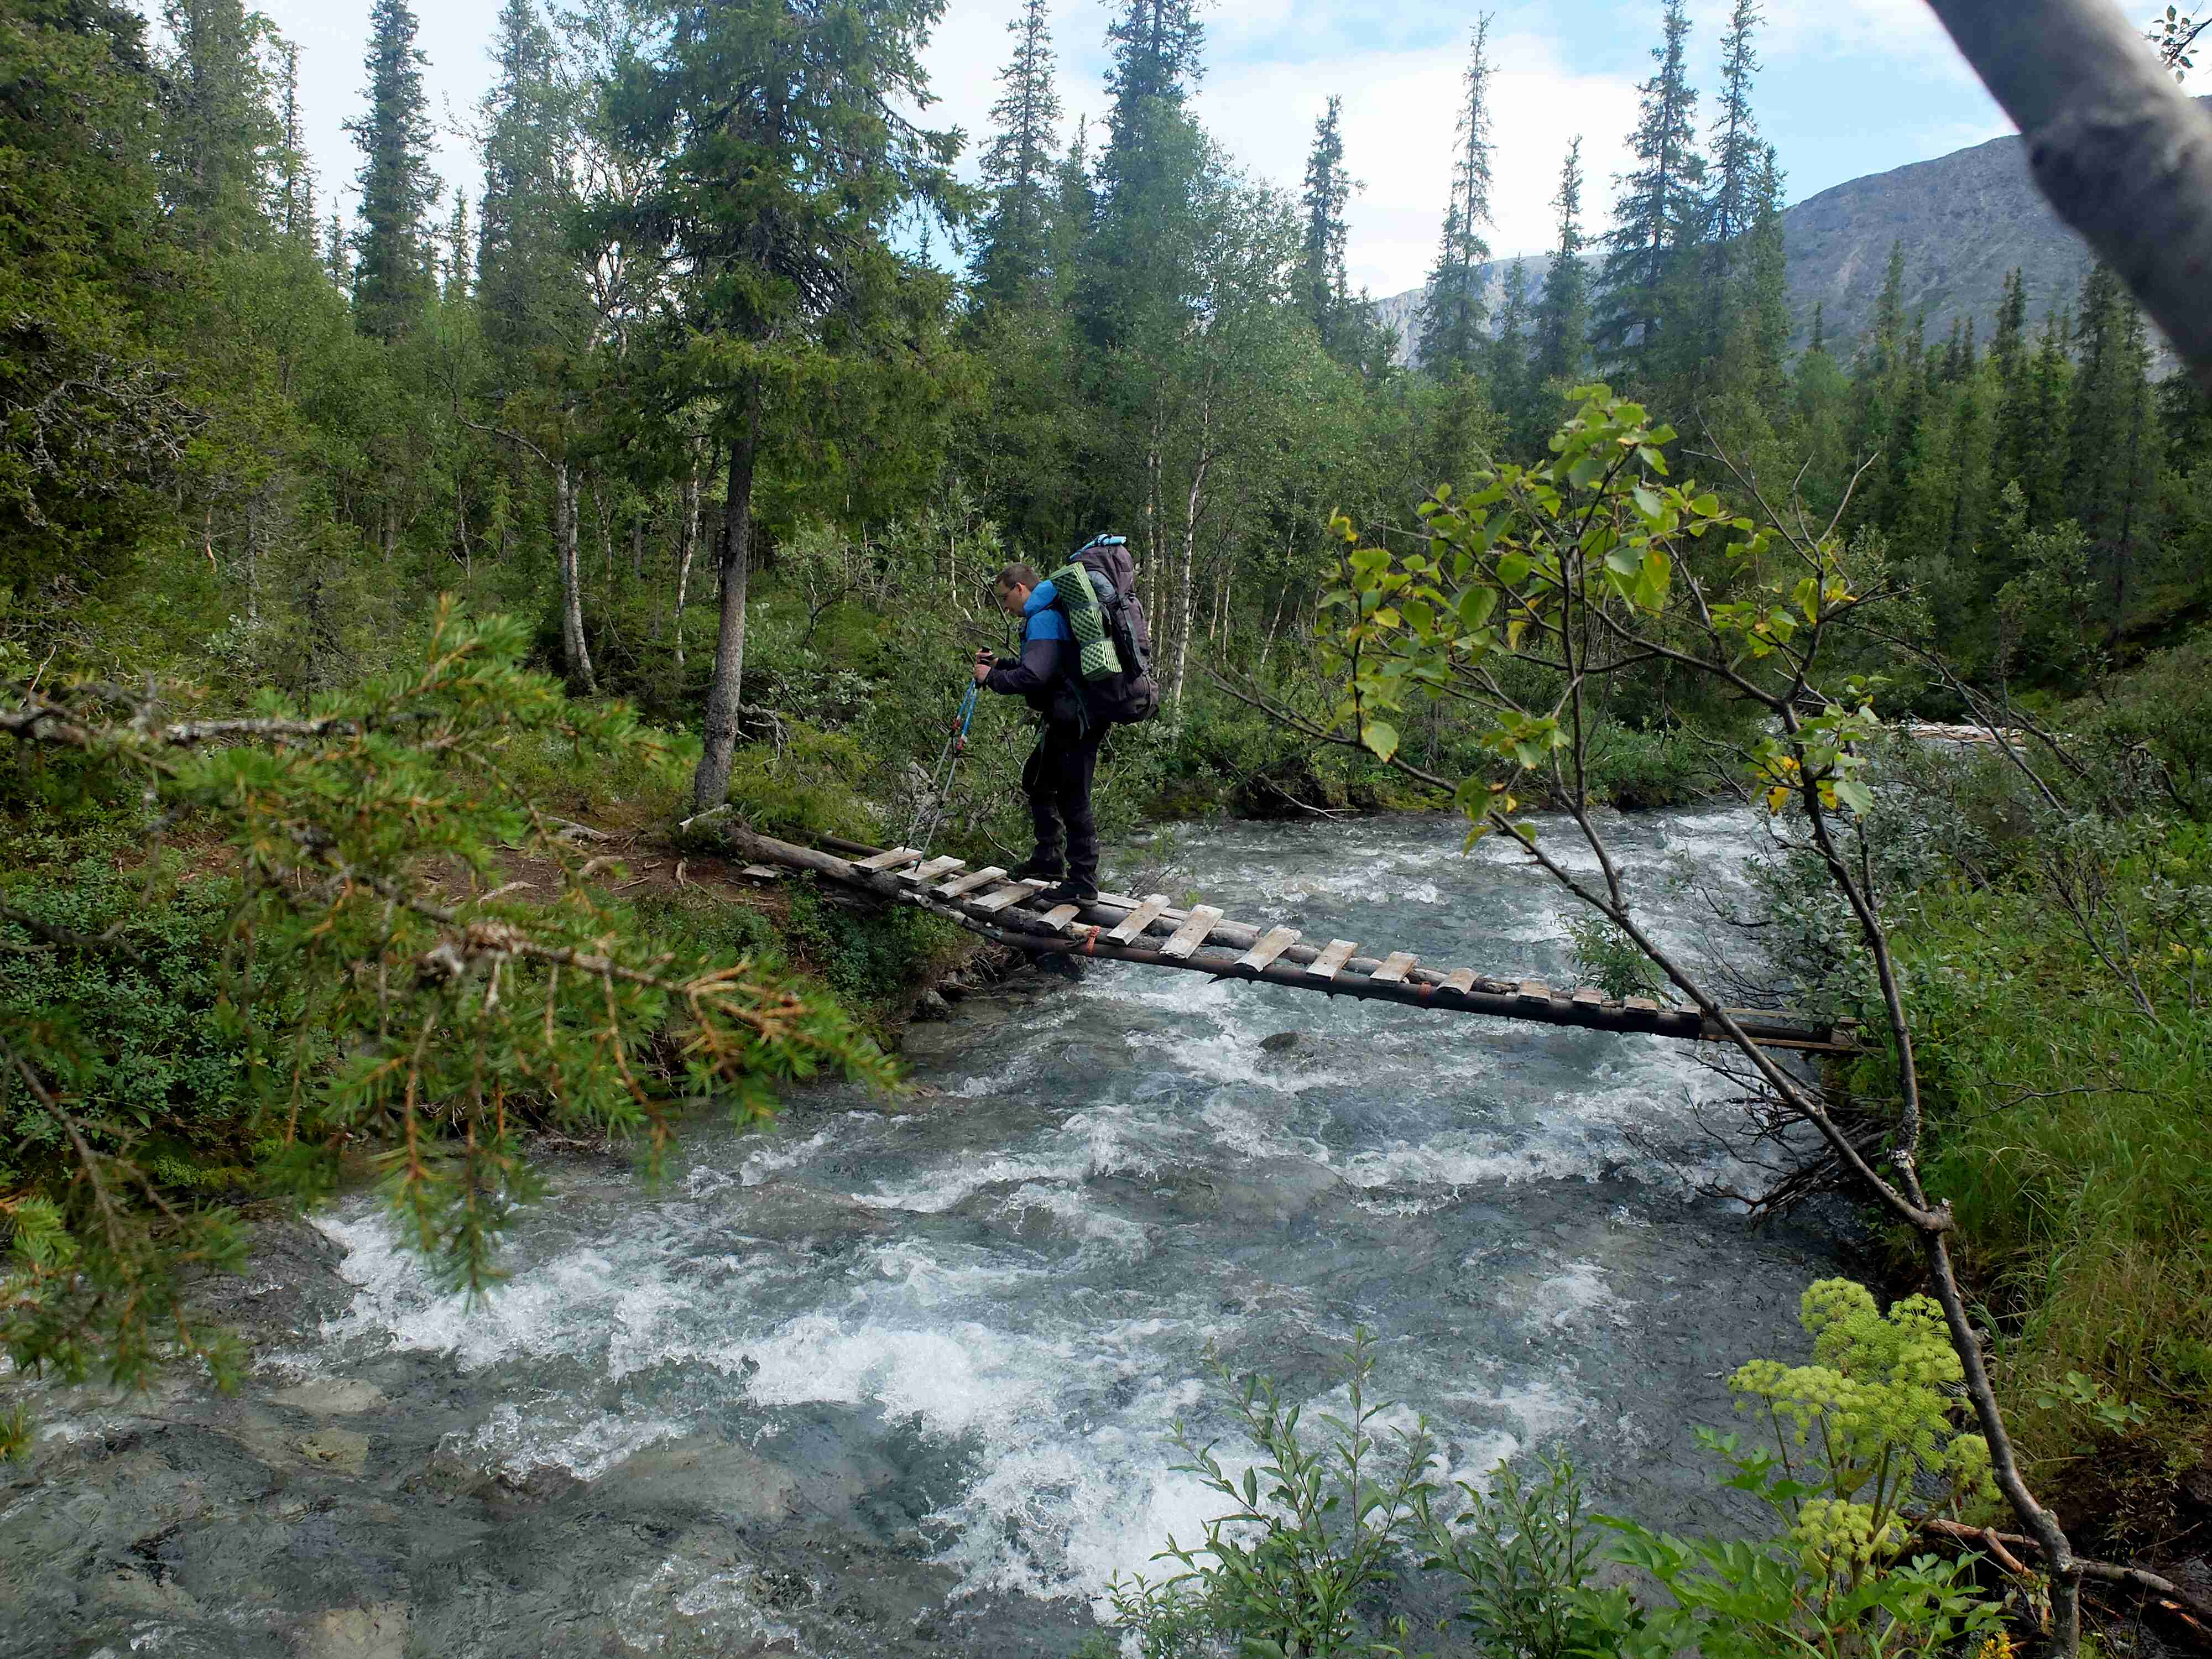
\includegraphics[width=14cm]{foto/09_08/01.Мост.png.jpg}
    \caption{Пешеходный мостик через руч. Петрелиуса}
    \label{fig5:1}
\end{figure}

\begin{figure}
    \centering
    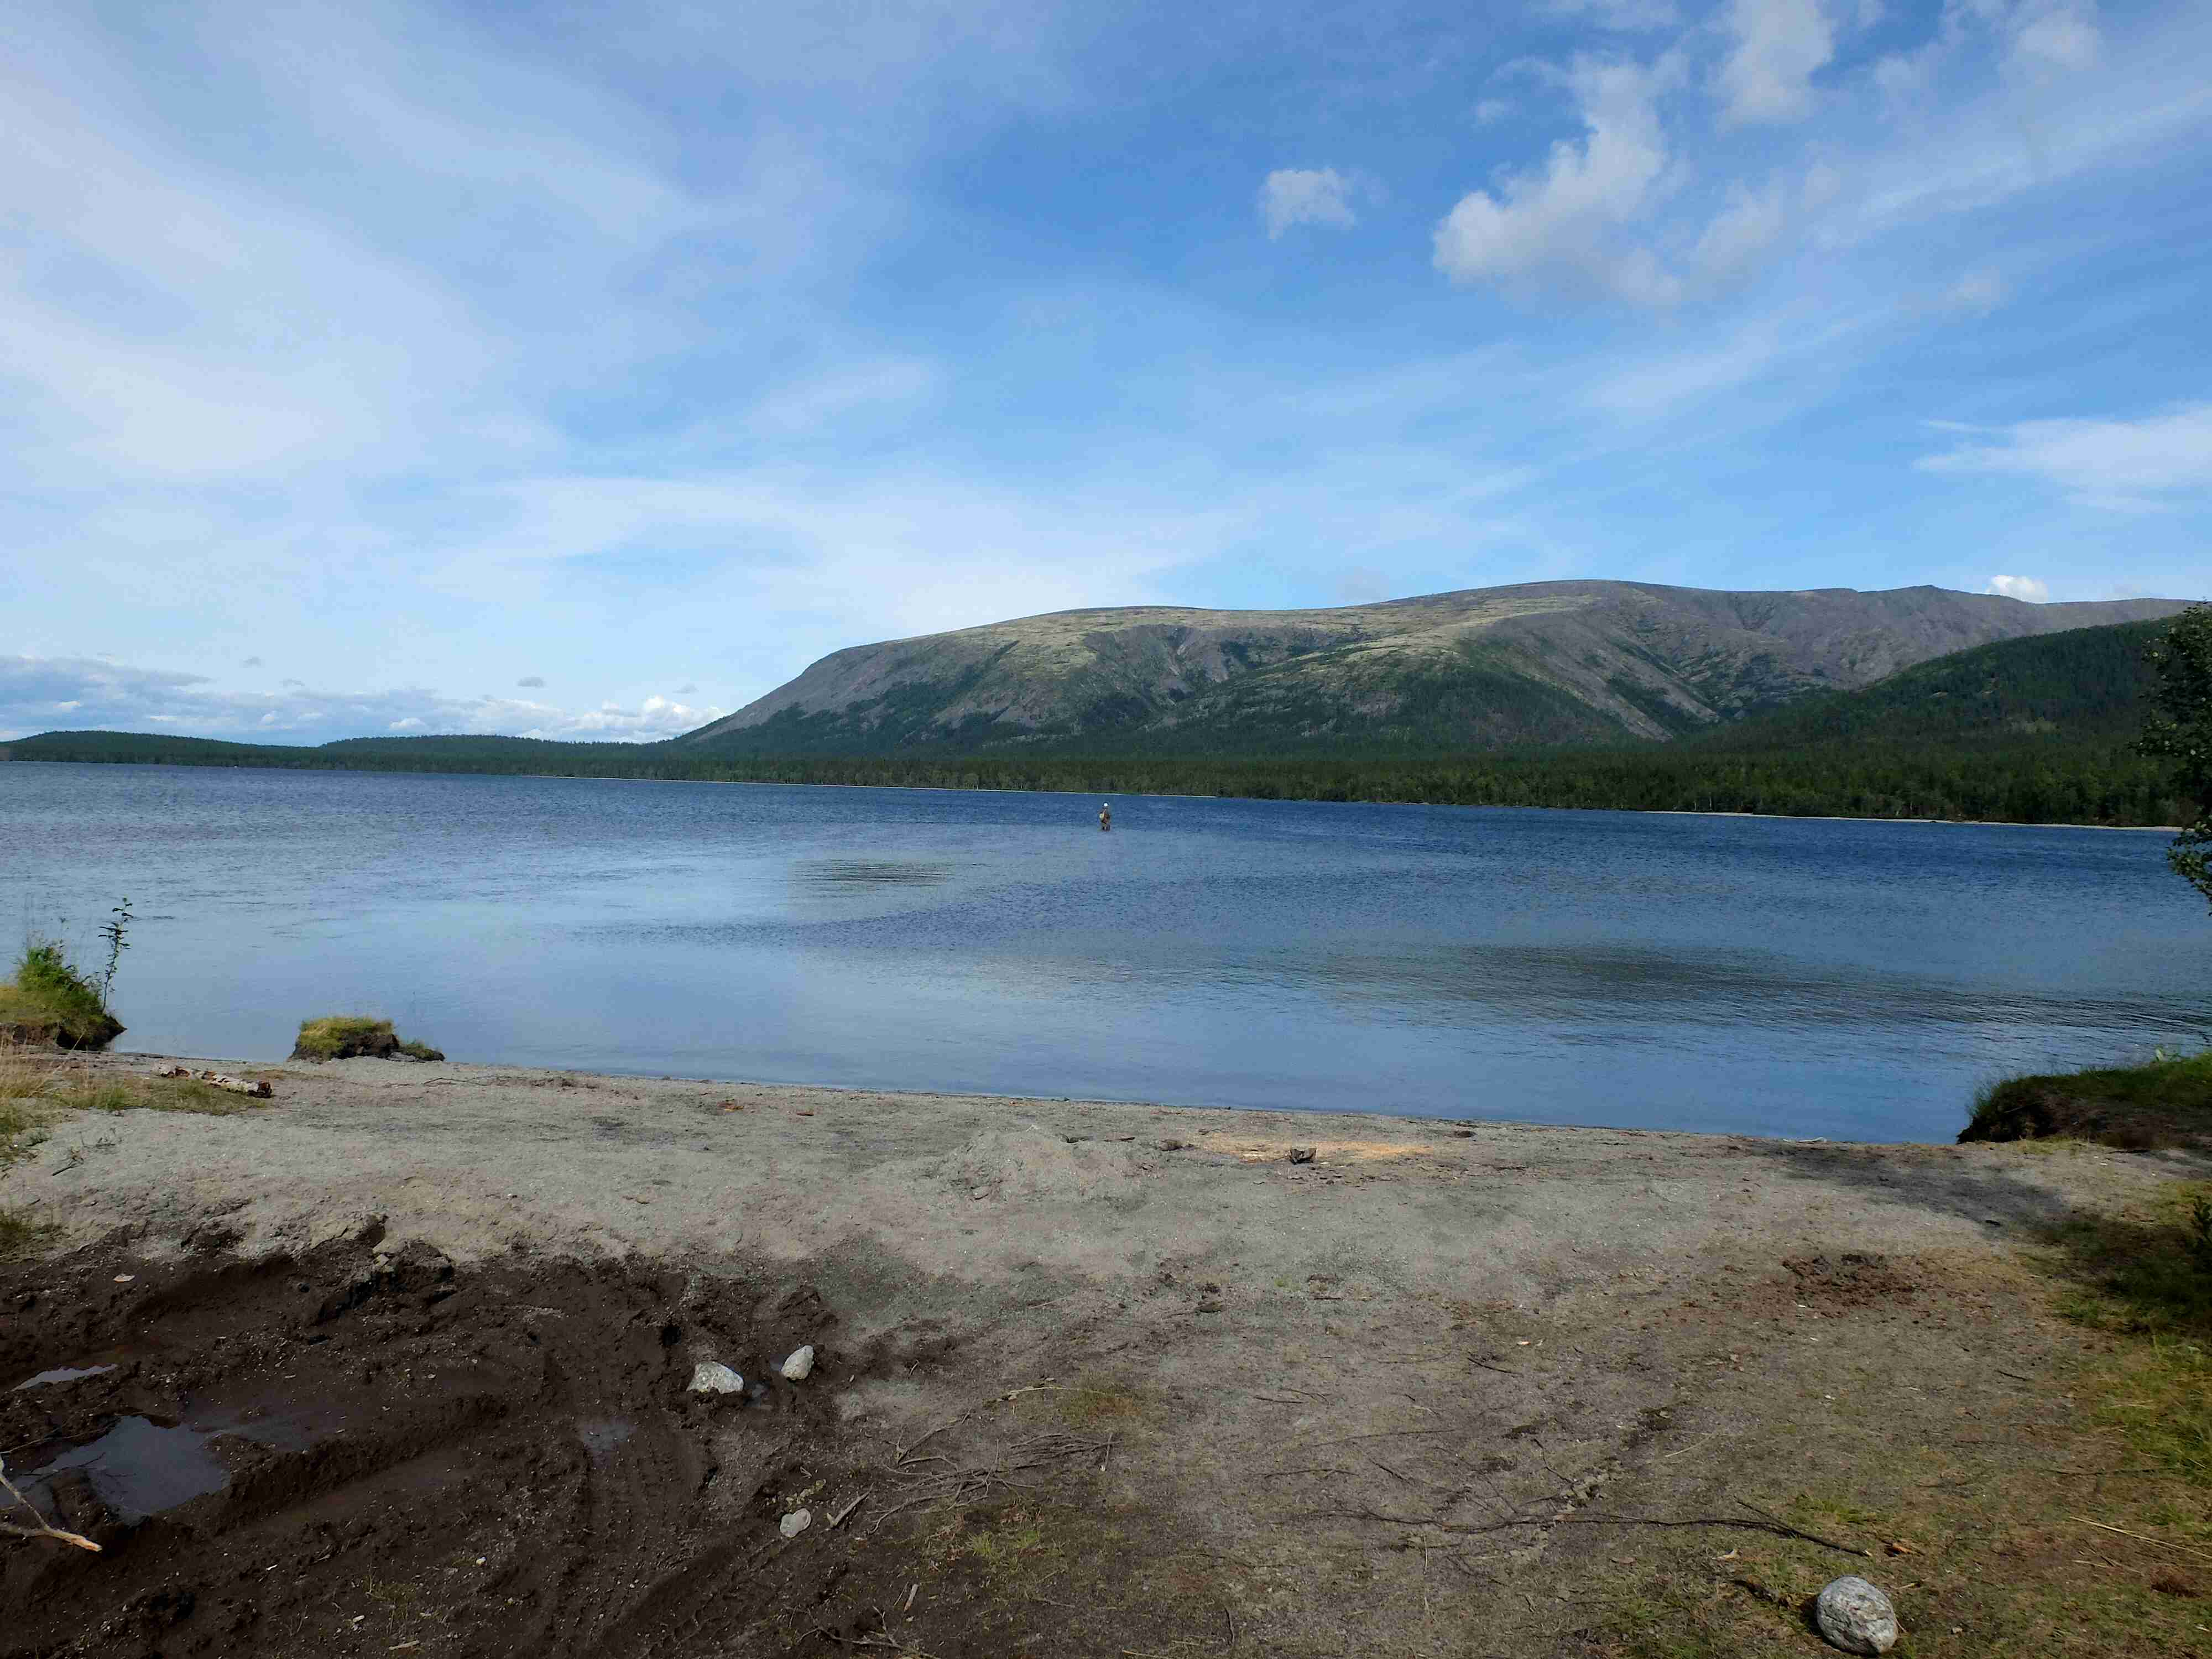
\includegraphics[width=14cm]{foto/09_08/02.Озеро Гольцовое.png.jpg}
    \caption{Оз. Гольцовое}
    \label{fig5:2}
\end{figure}

\begin{figure}
    \centering
    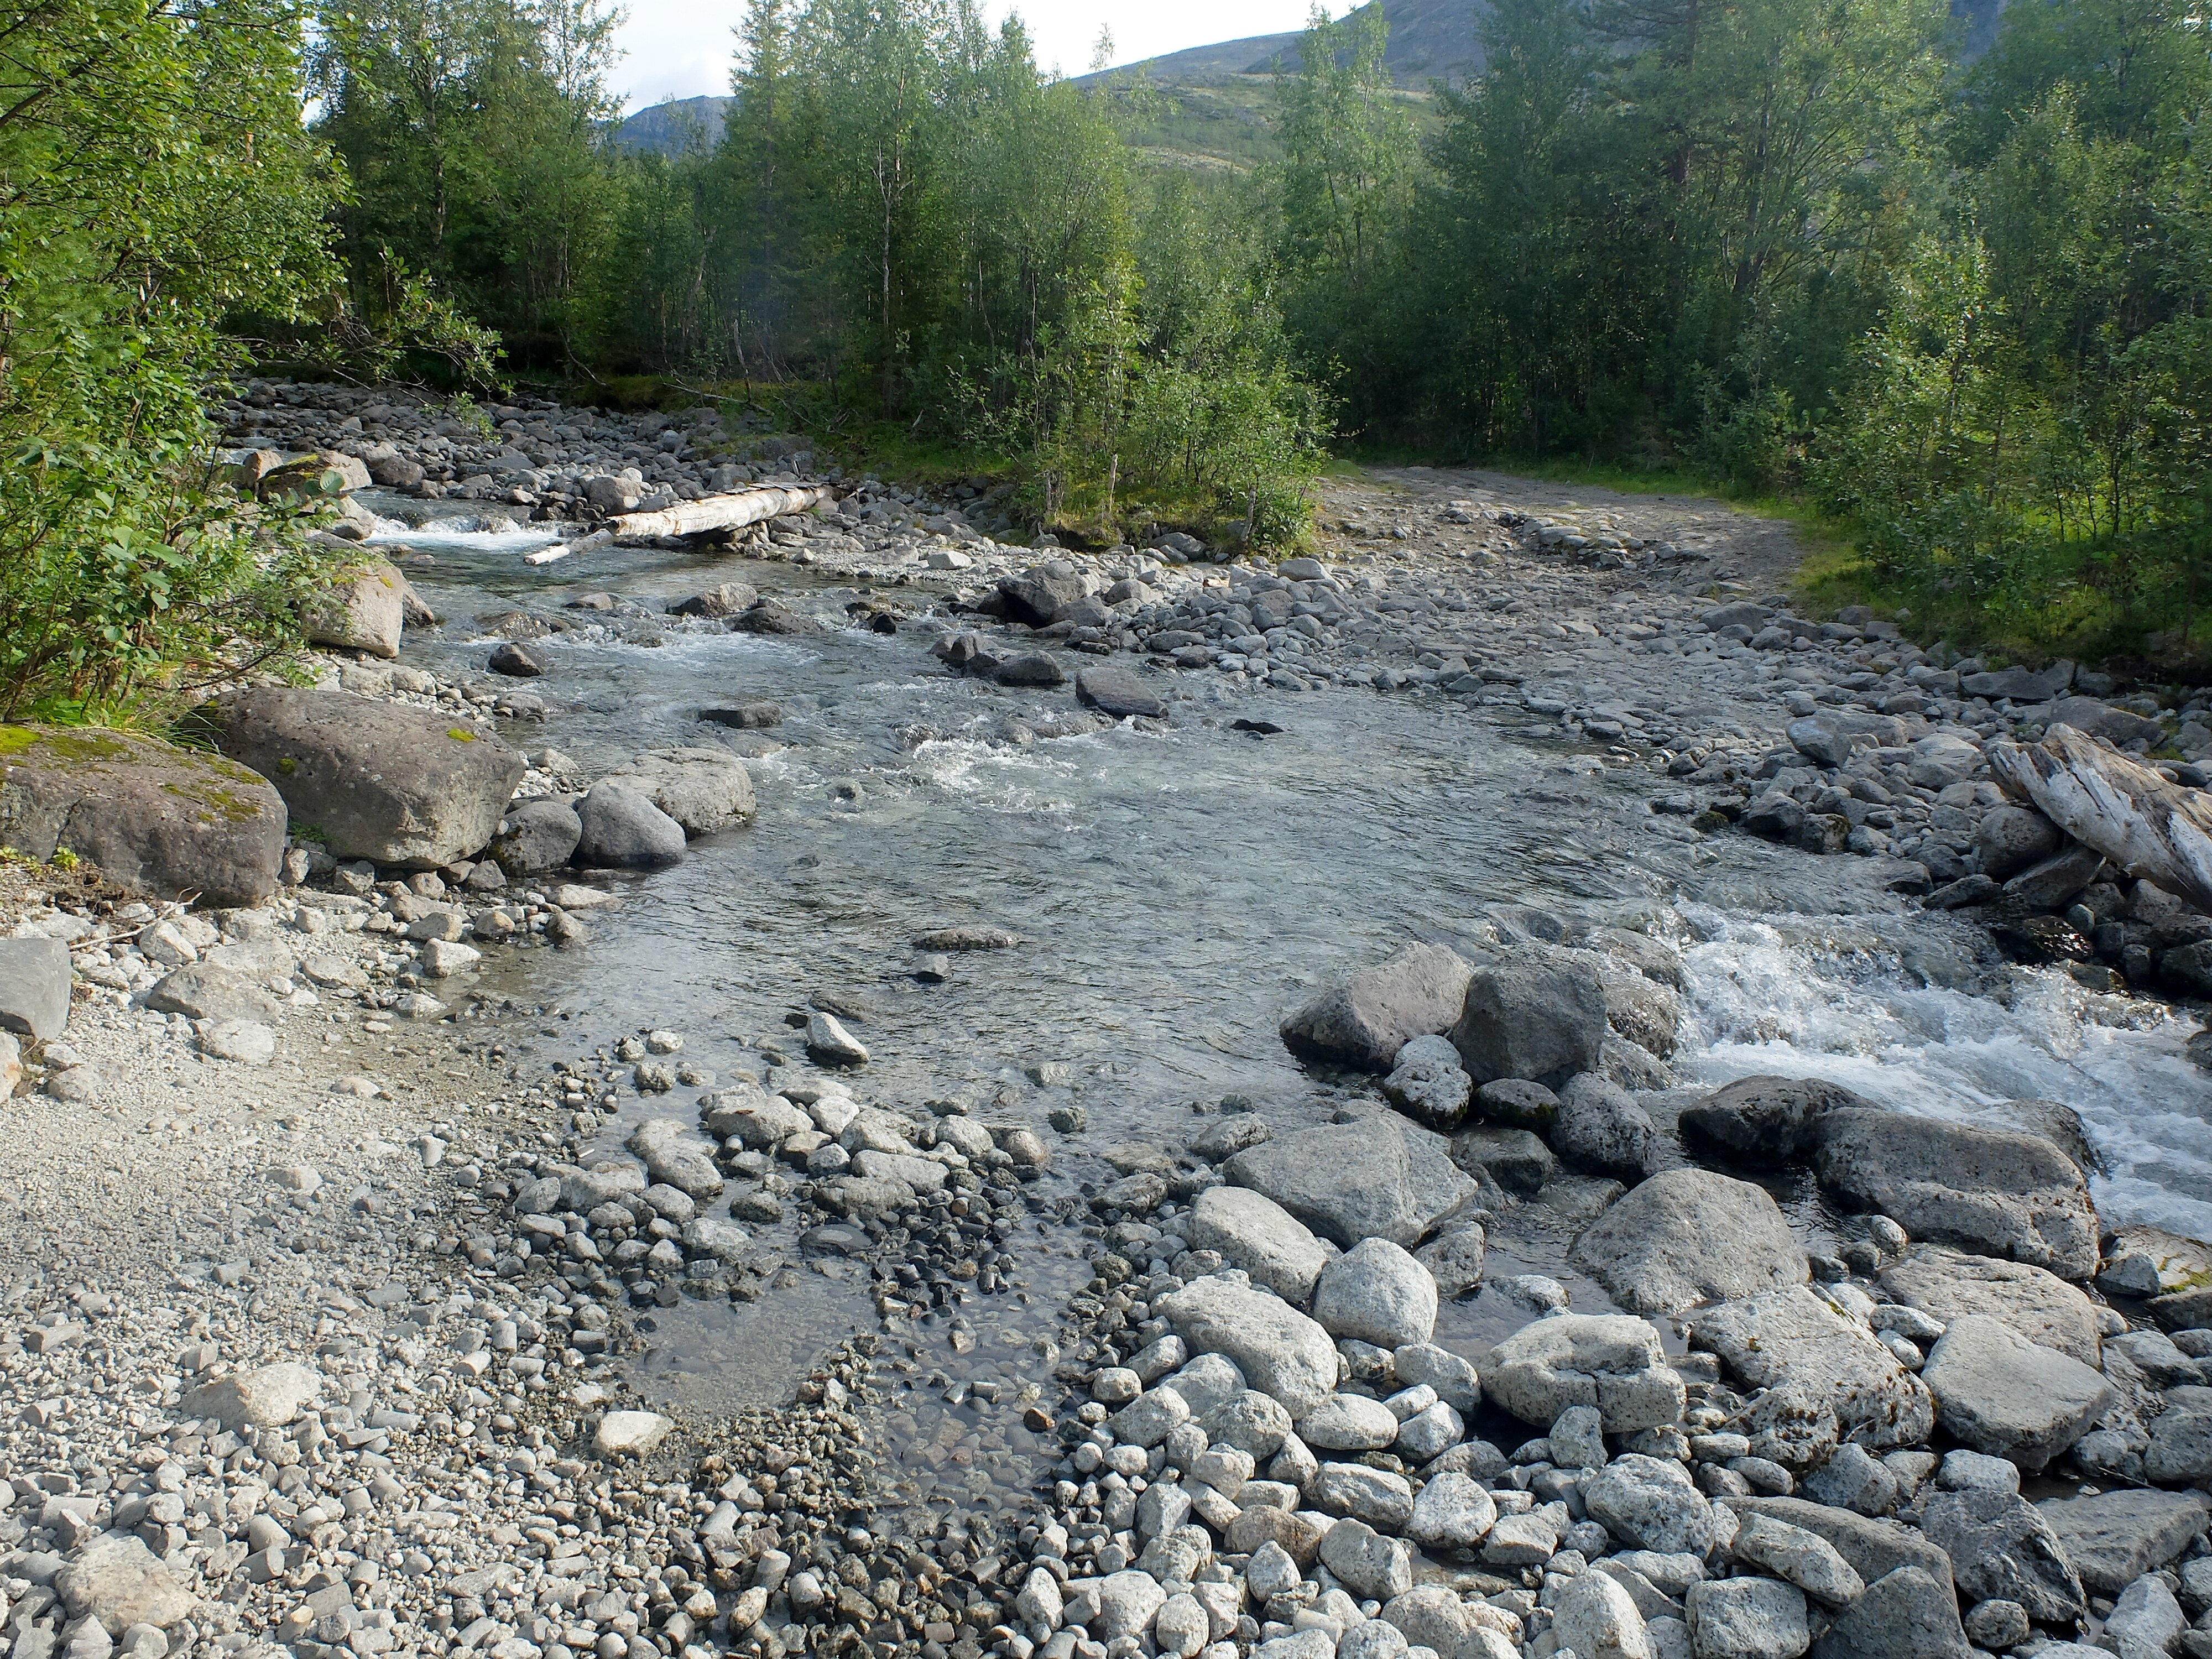
\includegraphics[width=14cm]{foto/09_08/03.Дорога на перевал.png.jpg}
    \caption{Дорога на пер. Умбозёрский}
    \label{fig5:3}
\end{figure}

\begin{figure}
    \centering
    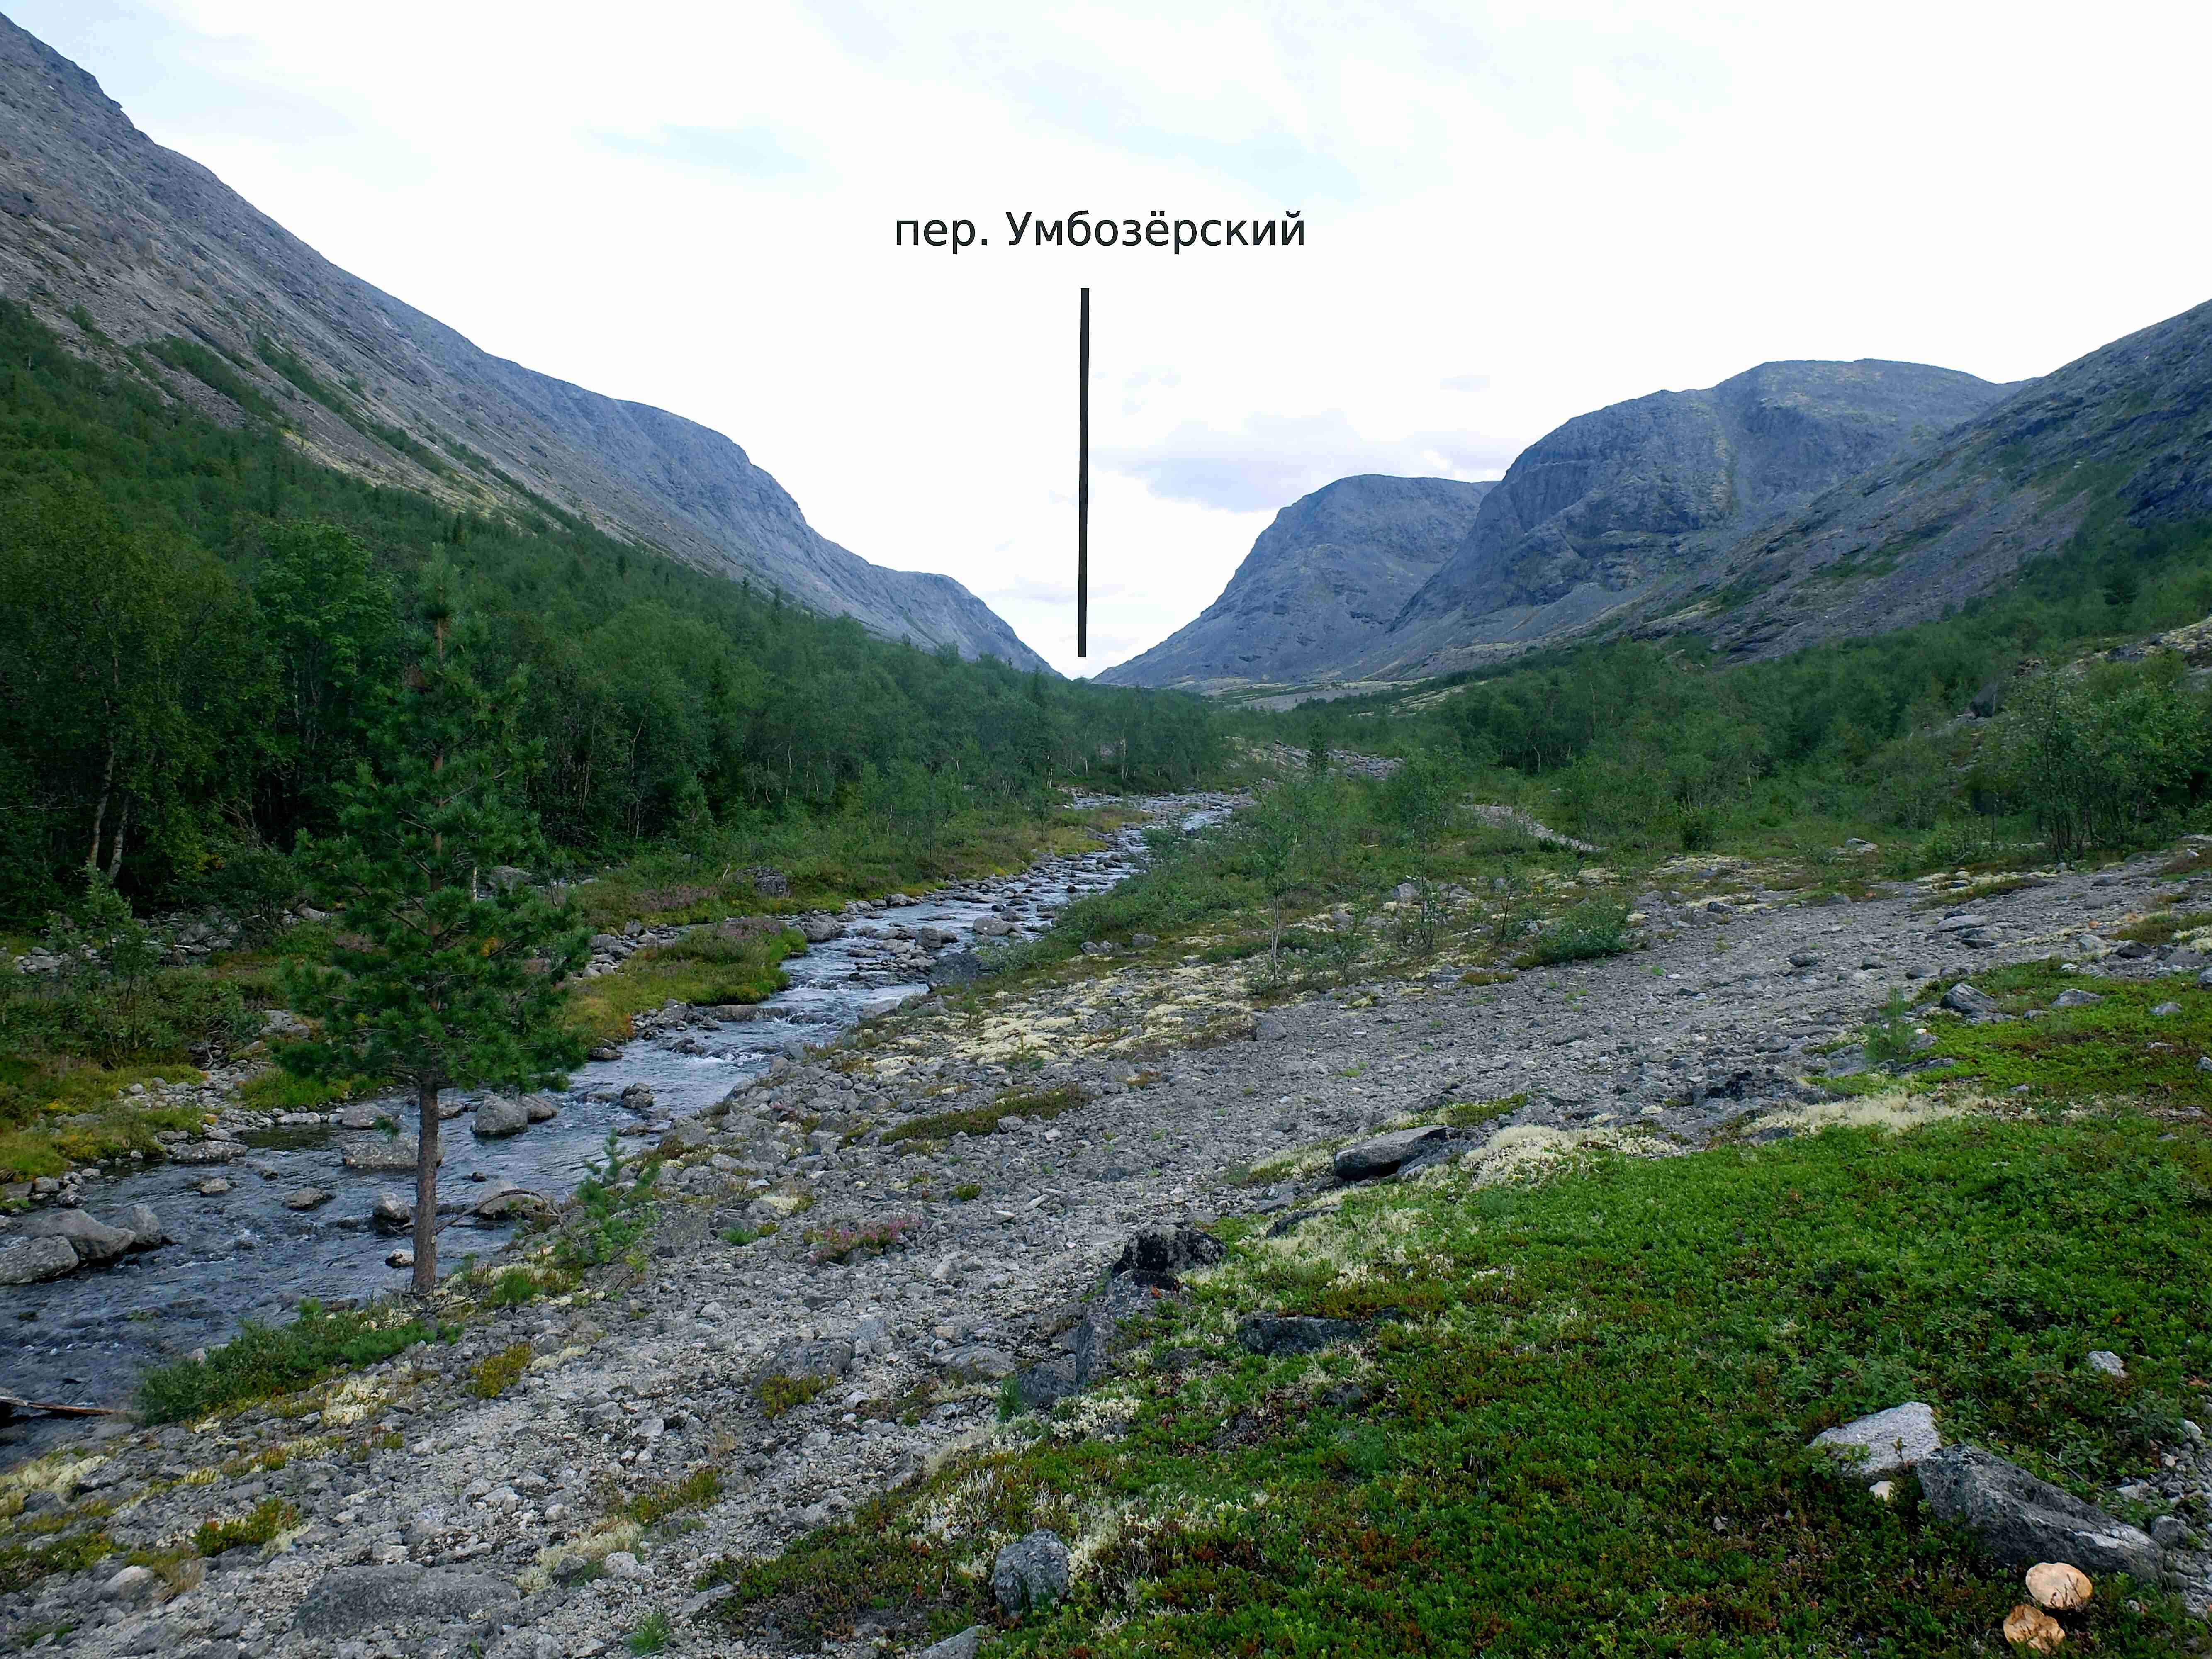
\includegraphics[width=14cm]{foto/09_08/04.Вид на перевал с запада.png.jpg}
    \caption{Вид на пер. Умбозёрский с запада}
    \label{fig5:4}
\end{figure}

\begin{figure}
    \centering
    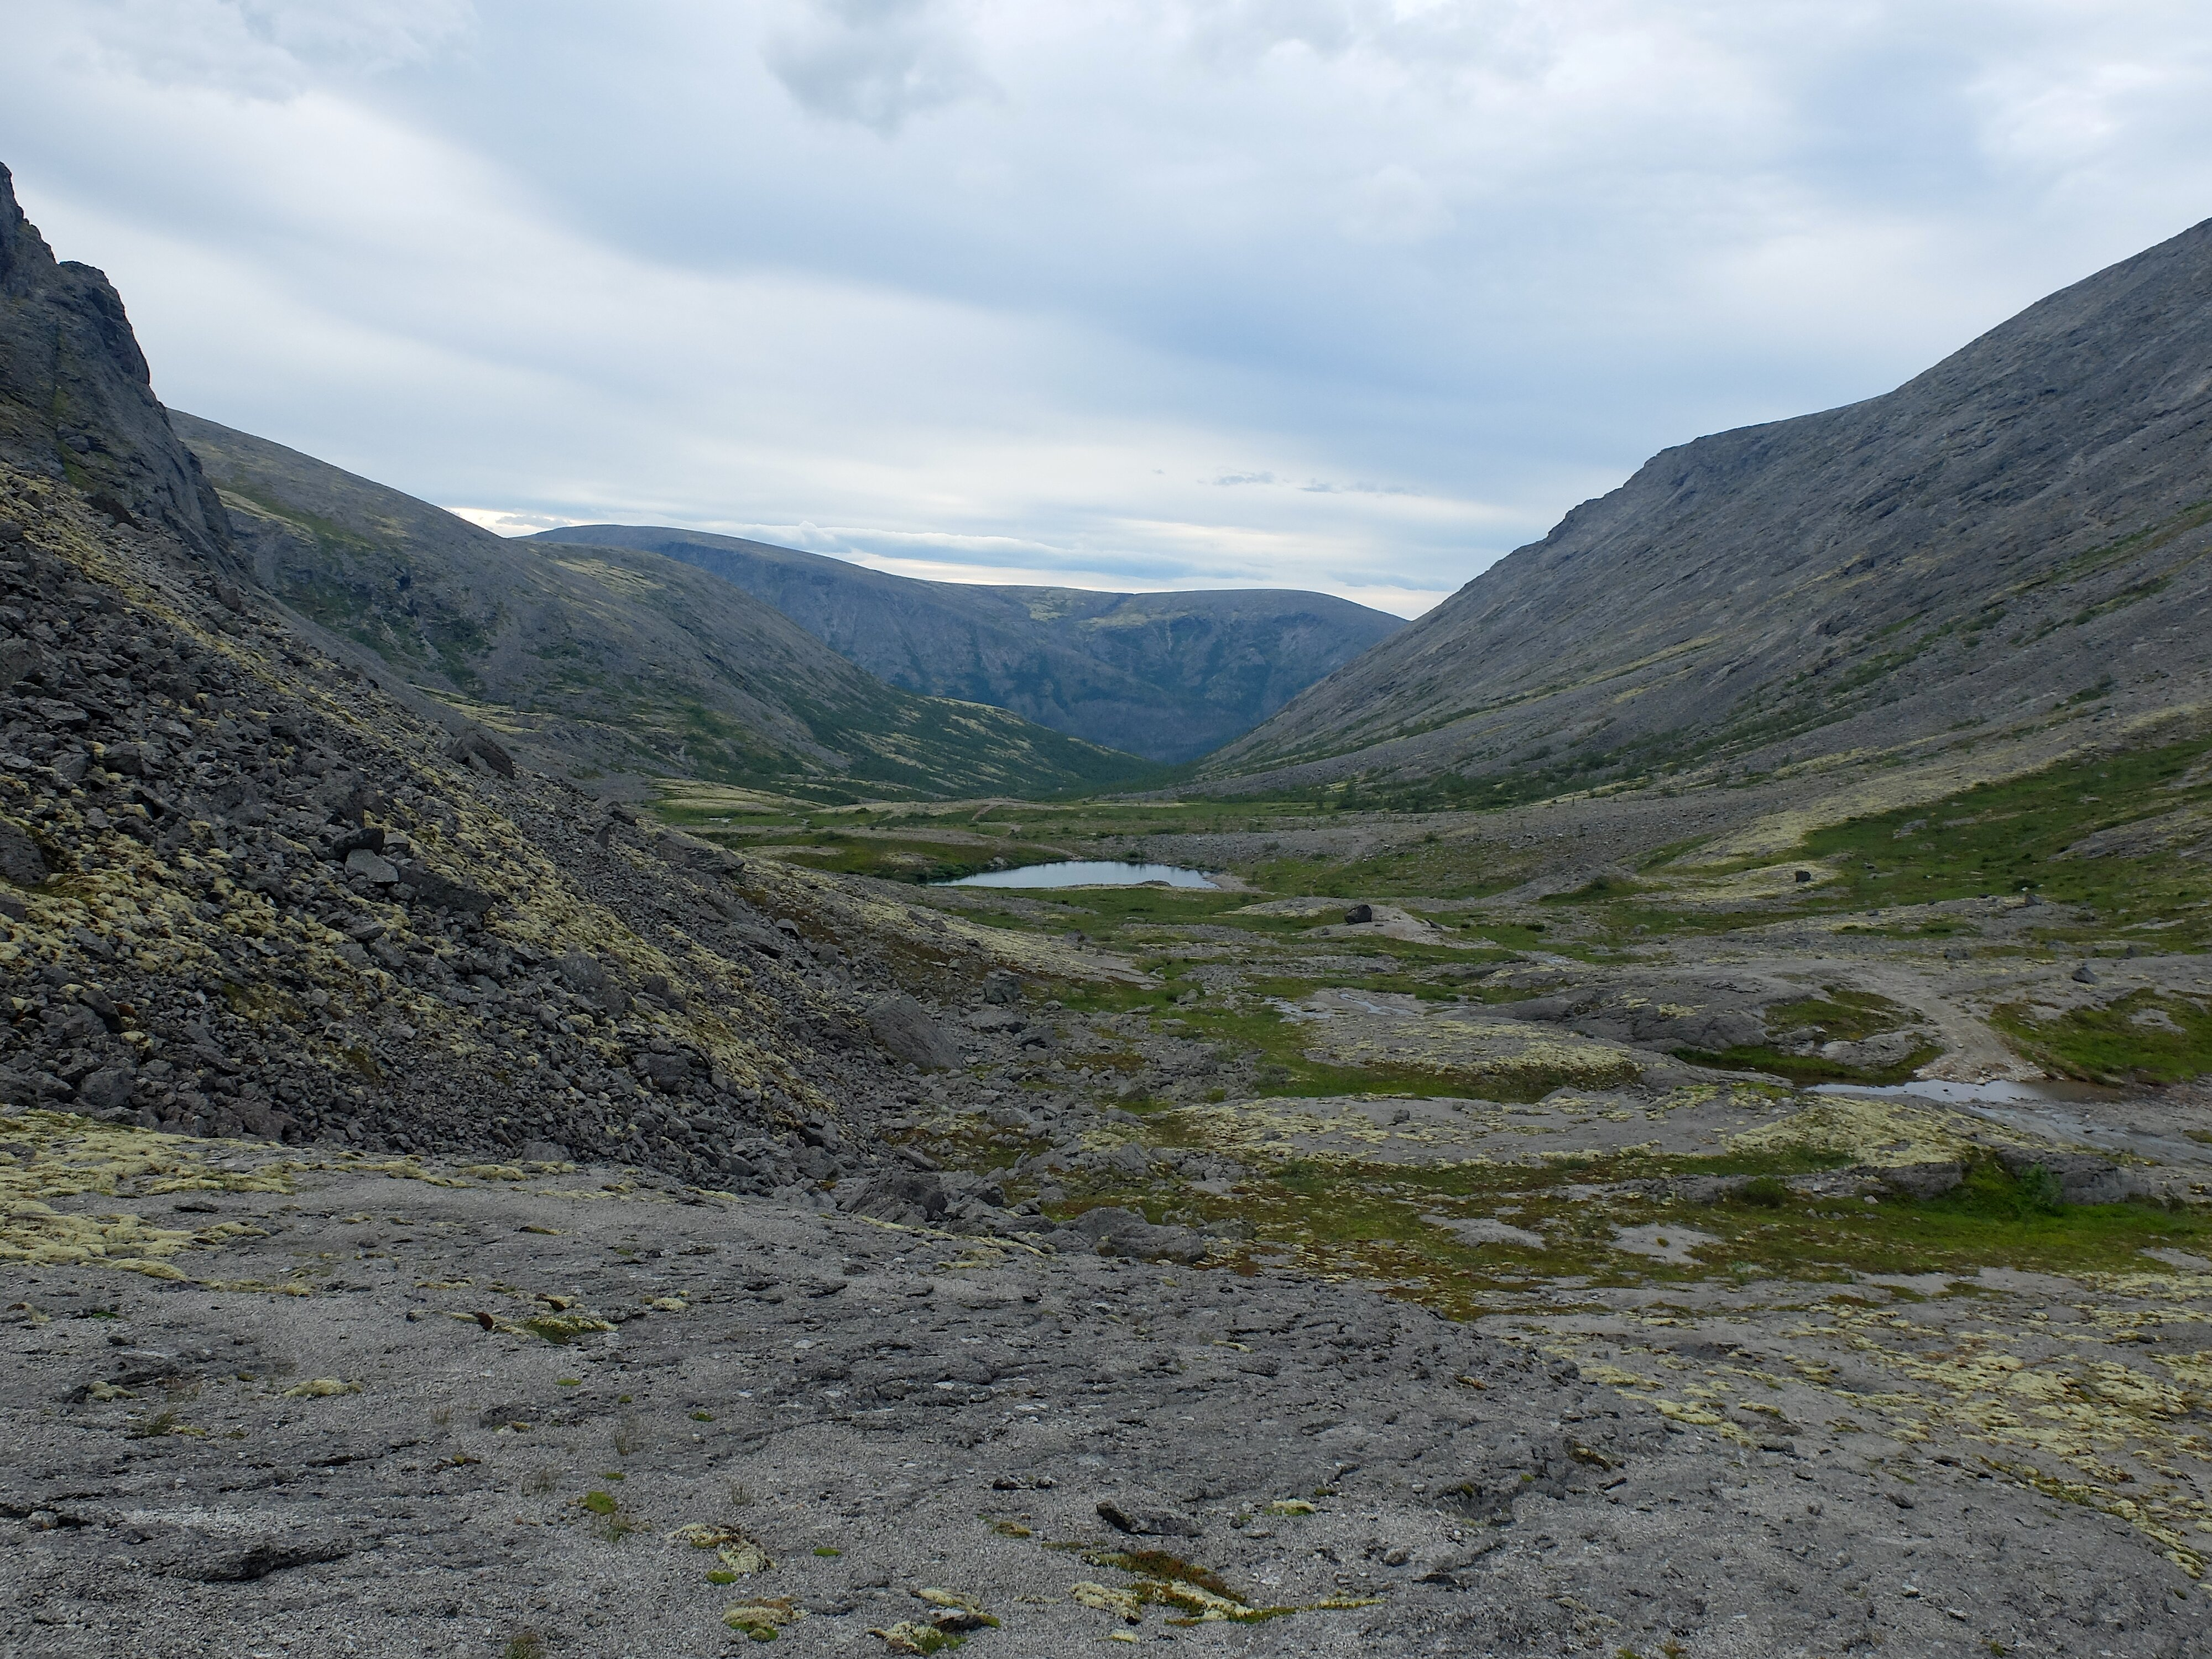
\includegraphics[width=14cm]{foto/09_08/05.Вид с перевала на восток.png.jpg}
    \caption{Вид с пер. Умбозёрский на восток}
    \label{fig5:5}
\end{figure}

\begin{figure}
    \centering
    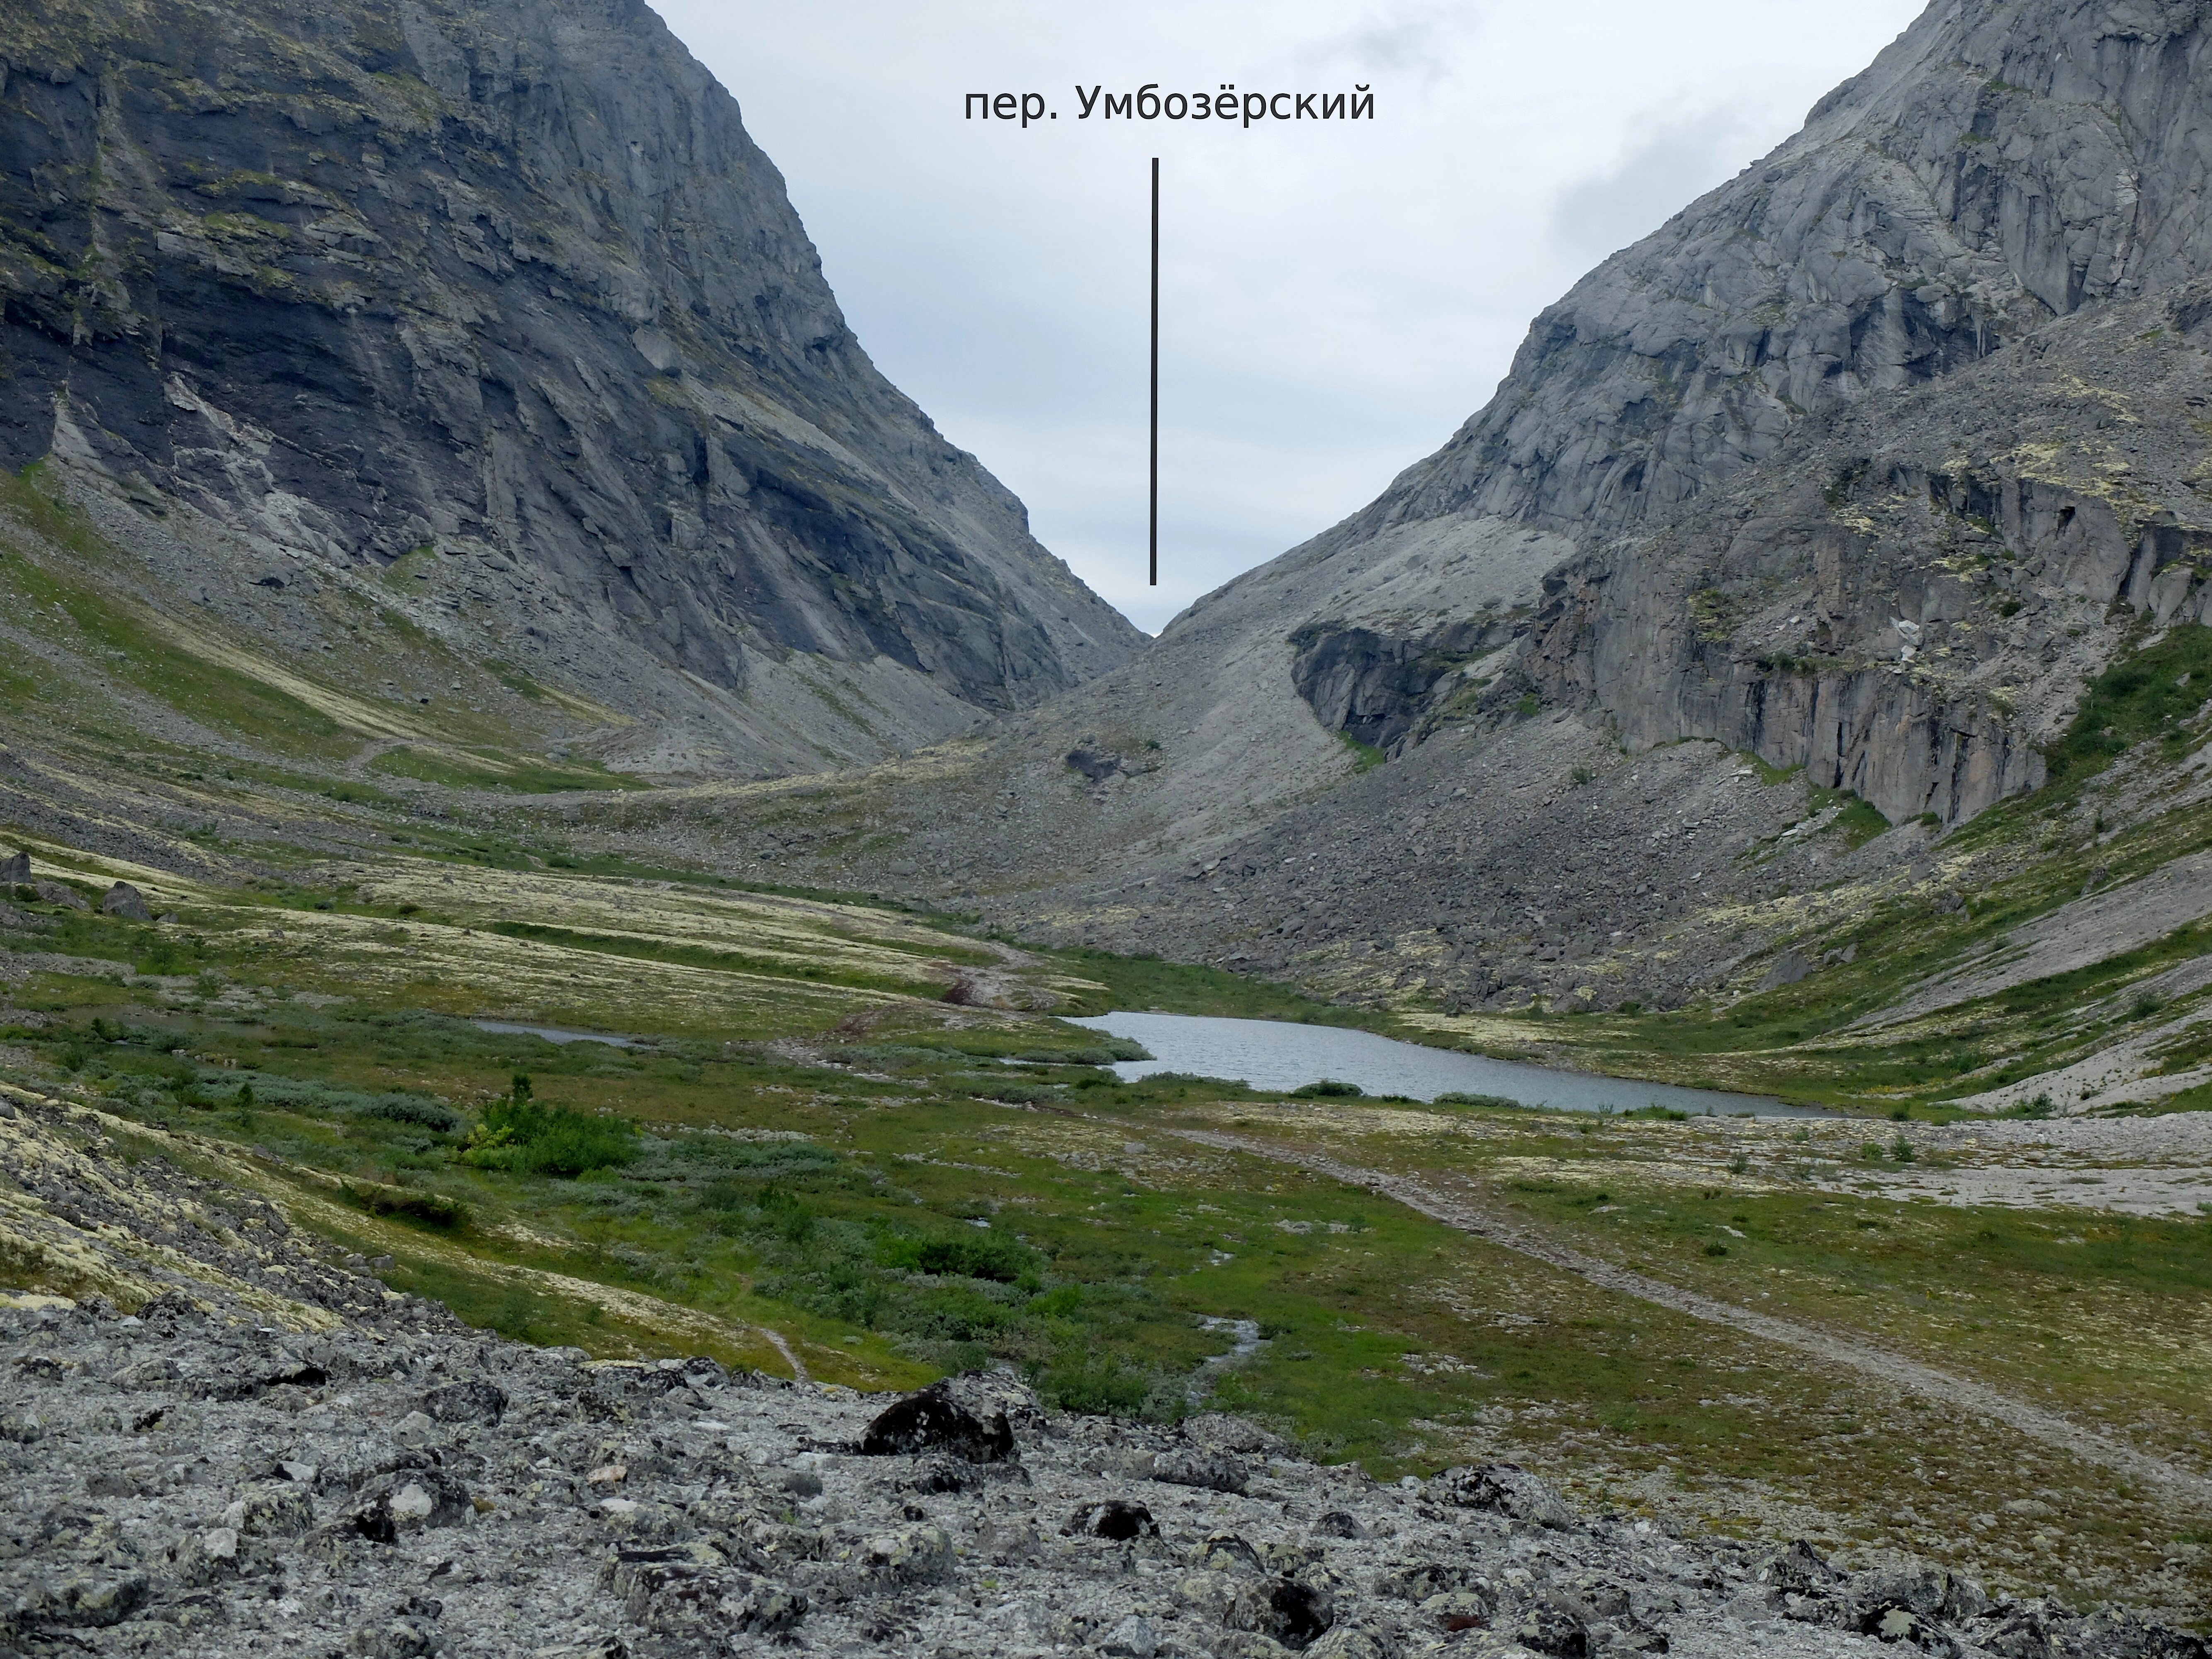
\includegraphics[width=14cm]{foto/09_08/06.Вид на перевал с востока.png.jpg}
    \caption{Вид на пер. Умбозёрский с востока}
    \label{fig5:6}
\end{figure}

\FloatBarrier

\subsection{День 6. 10.08.2022\\
Р. Северный Каскаснюнйок -- р. Каскаснюнйок -- переправа р. Каскаснюнйок}
\begin{tabular}{l p{12cm}}
\hline
Пройдено: & 13.21 км\\
Набор/сброс высоты: & 146/447 м\\
Время в пути: & 6:41\\
ЧХВ: & 3:53\\
Метеоусловия: & Облачно, без солнца\\
\hline
\end{tabular}

08:10 Подъём.
Погода облачная, +19$\tccentigrade$. Ветер, который сдувал нас за ужином, затих сразу после отбоя.
Далее весь так же облачно, без солнца.

10:58 Выходим (рис. \ref{fig6:1}).
Идём сначала по автомобильной дороге, вдоль р. Северный Каскаснюнйок. Чем ниже спускаемся, тем шире река,
и тем чаще автодорога идёт просто по руслу. С какого-то момента, устав от бродов, находим на левом берегу тропу
и идём уже по ней (рис. \ref{fig6:2}). Примерно там же начинается редкий лес, по мере спуска усиливается, но всё равно проходим.

Незадолго до слияния с р. Южный Каскаснюнйок наша тропа утыкается в автодорогу.
Дорога болотистая, часто лужи на всю ширину дороги, часто месиво из земли, причём слой почвы высокий --- глубоко проваливаешься,
приходится обходить параллельно через лесок (рис. \ref{fig6:3}). Связана эта заболоченность, видимо, со множеством ручьёв,
стекающих со склонов горной гряды (верш. Партомпорр) по левую руку.

15:34 Наконец доходим до ответвления на брод, тут --- площадки под стоянки, питьевой ручеёк, текущий параллельно Каскаснюнйоку.
Становимся на обед.

17:35 Собираемся духом (как же, категорийная переправа (по описаниям)), надеваем бродовые кроссовки,
убираем важное в гермомешки. Но переправляемся легко. Сначала мелкое русло по щиколотку, течение не ощущается.
Затем основное русло, скорость течения --- 1 м/с, глубина --- по колено (0.5 метра), ширина --- метров 10 (рис. \ref{fig6:4}).
Переходим по одному.

В 100 метрах от переправы большая поляна со стоянками. Ставимся. Поскольку ужинать рано --- отдыхаем.

21:00 Ужинаем.

22:30 Отбой. t=+17$\tccentigrade$.

\begin{figure}
    \centering
    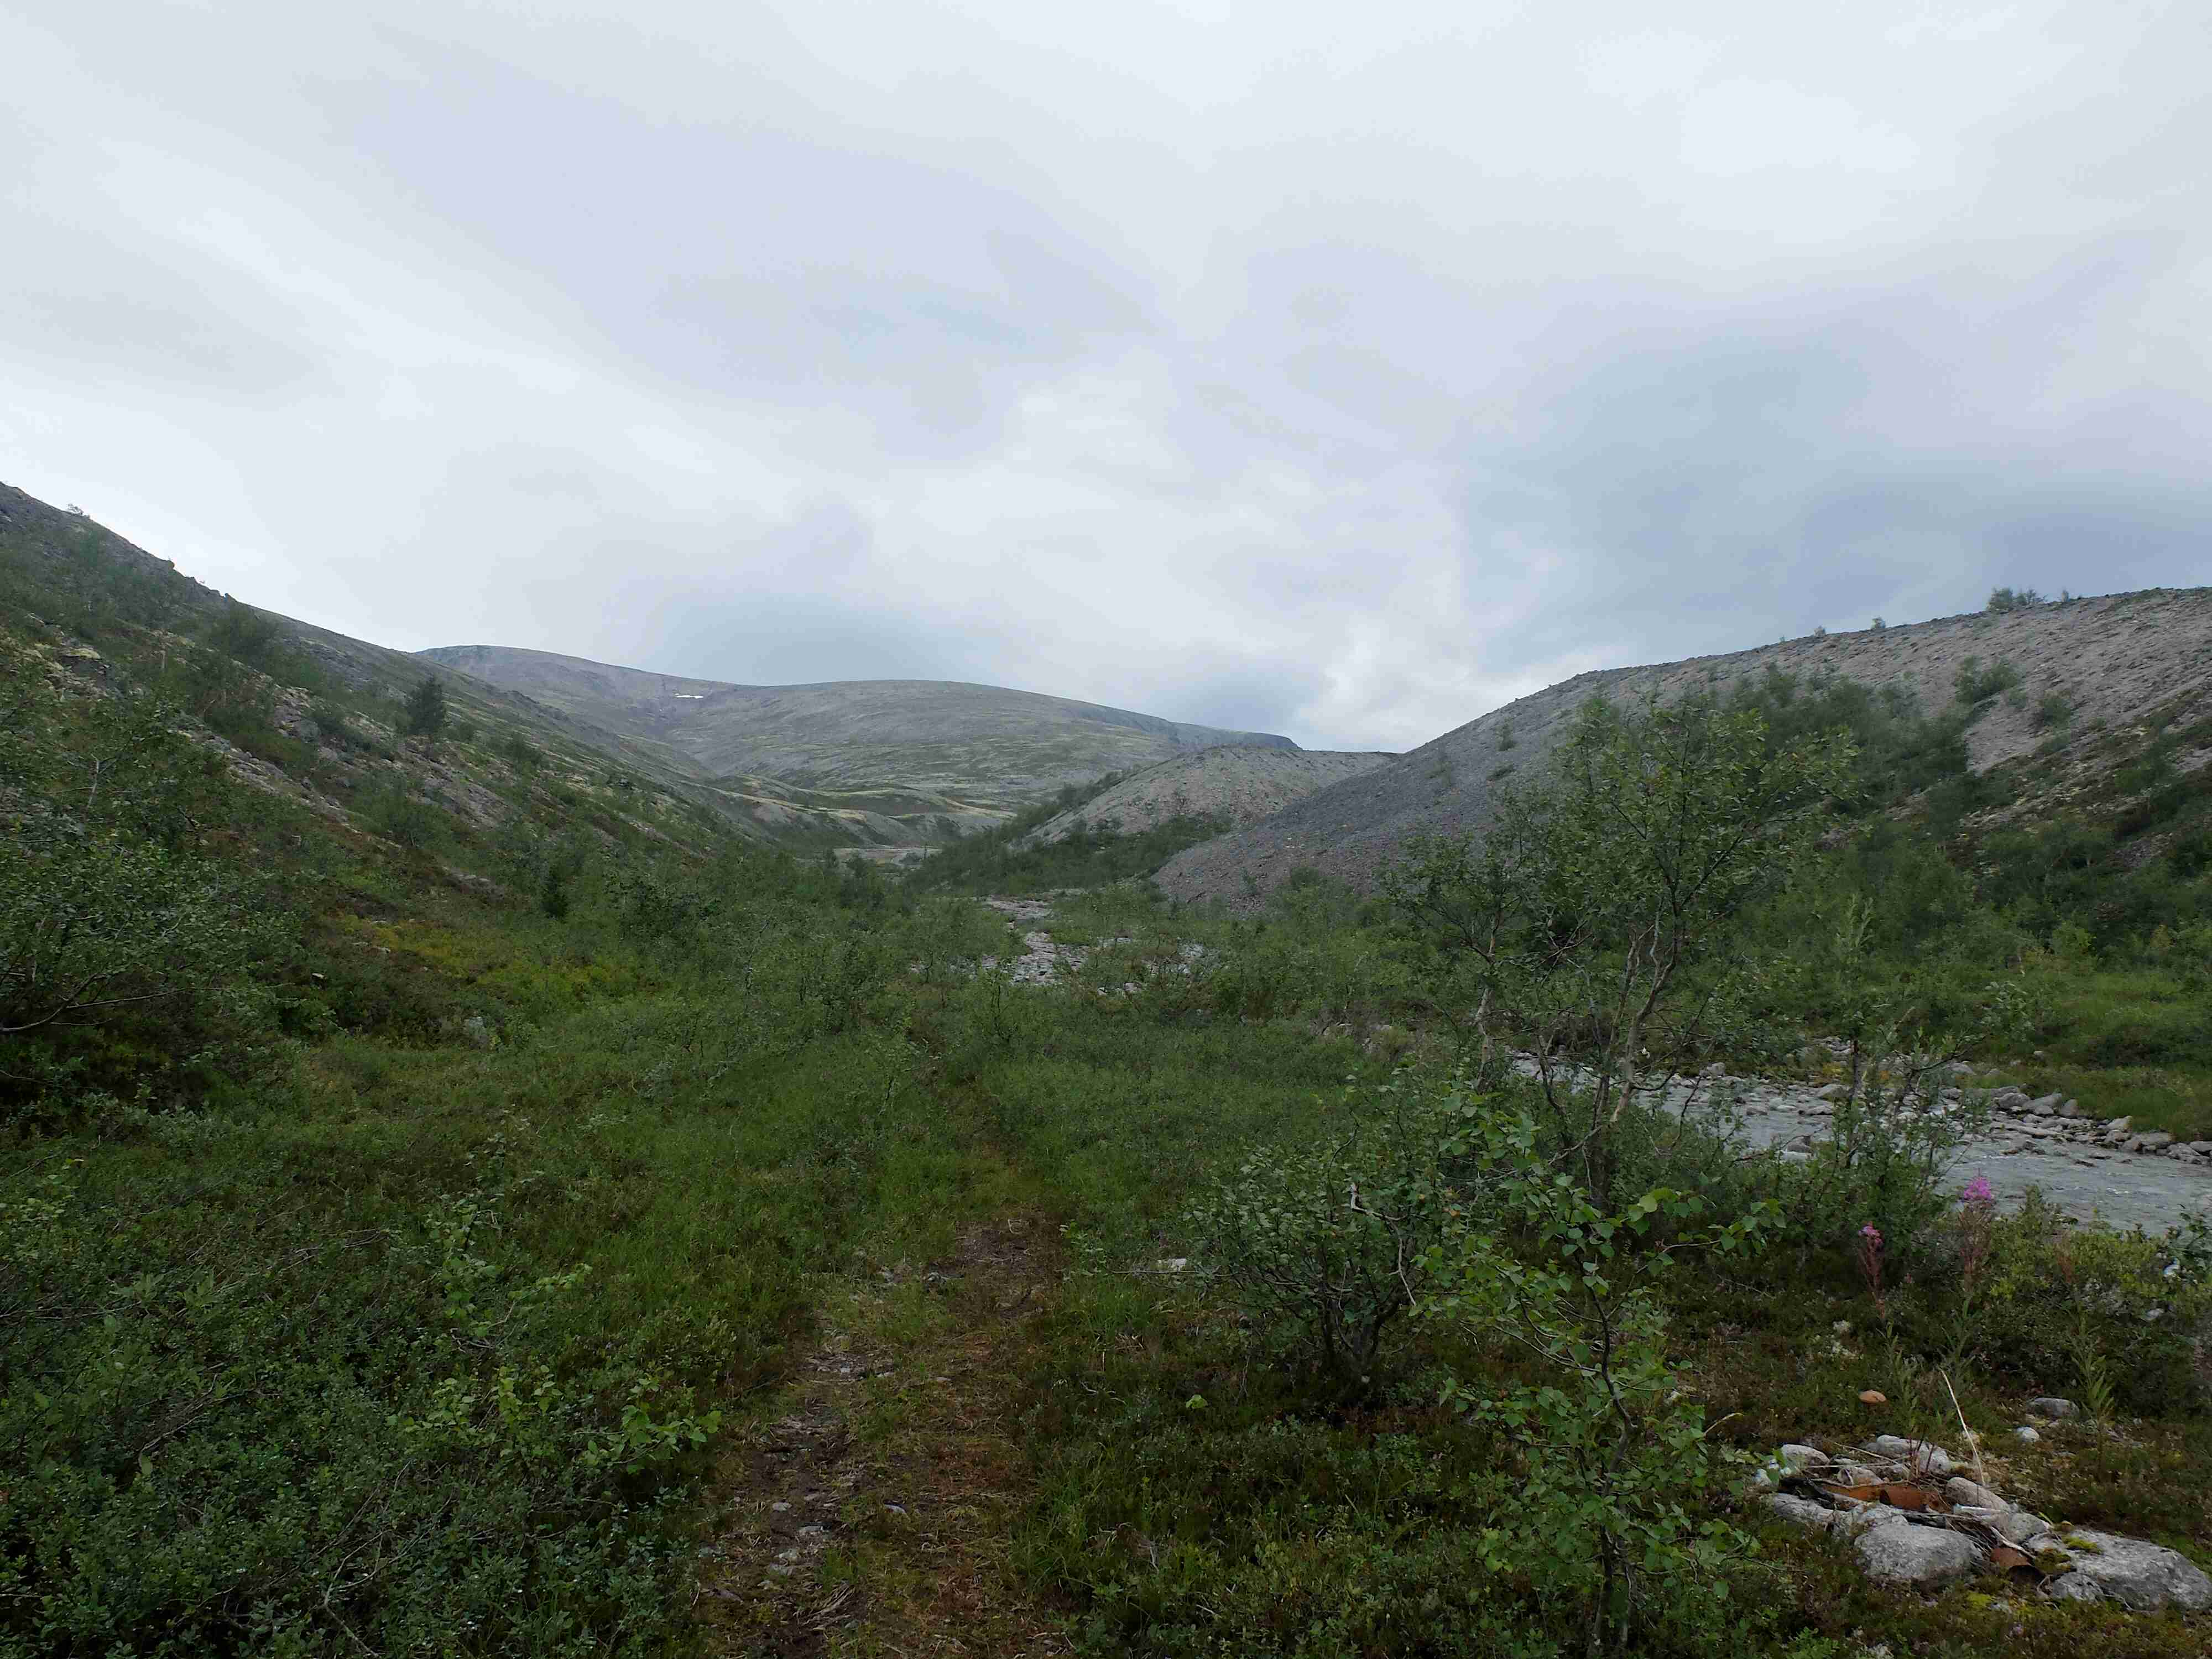
\includegraphics[width=14cm]{foto/10_08/02.Тропинка с перевала вдоль дороги.png.jpg}
    \caption{Тропа от пер. Умбозёрский вдоль р. Северный Каскаснюнйок}
    \label{fig6:1}
\end{figure}

\begin{figure}
    \centering
    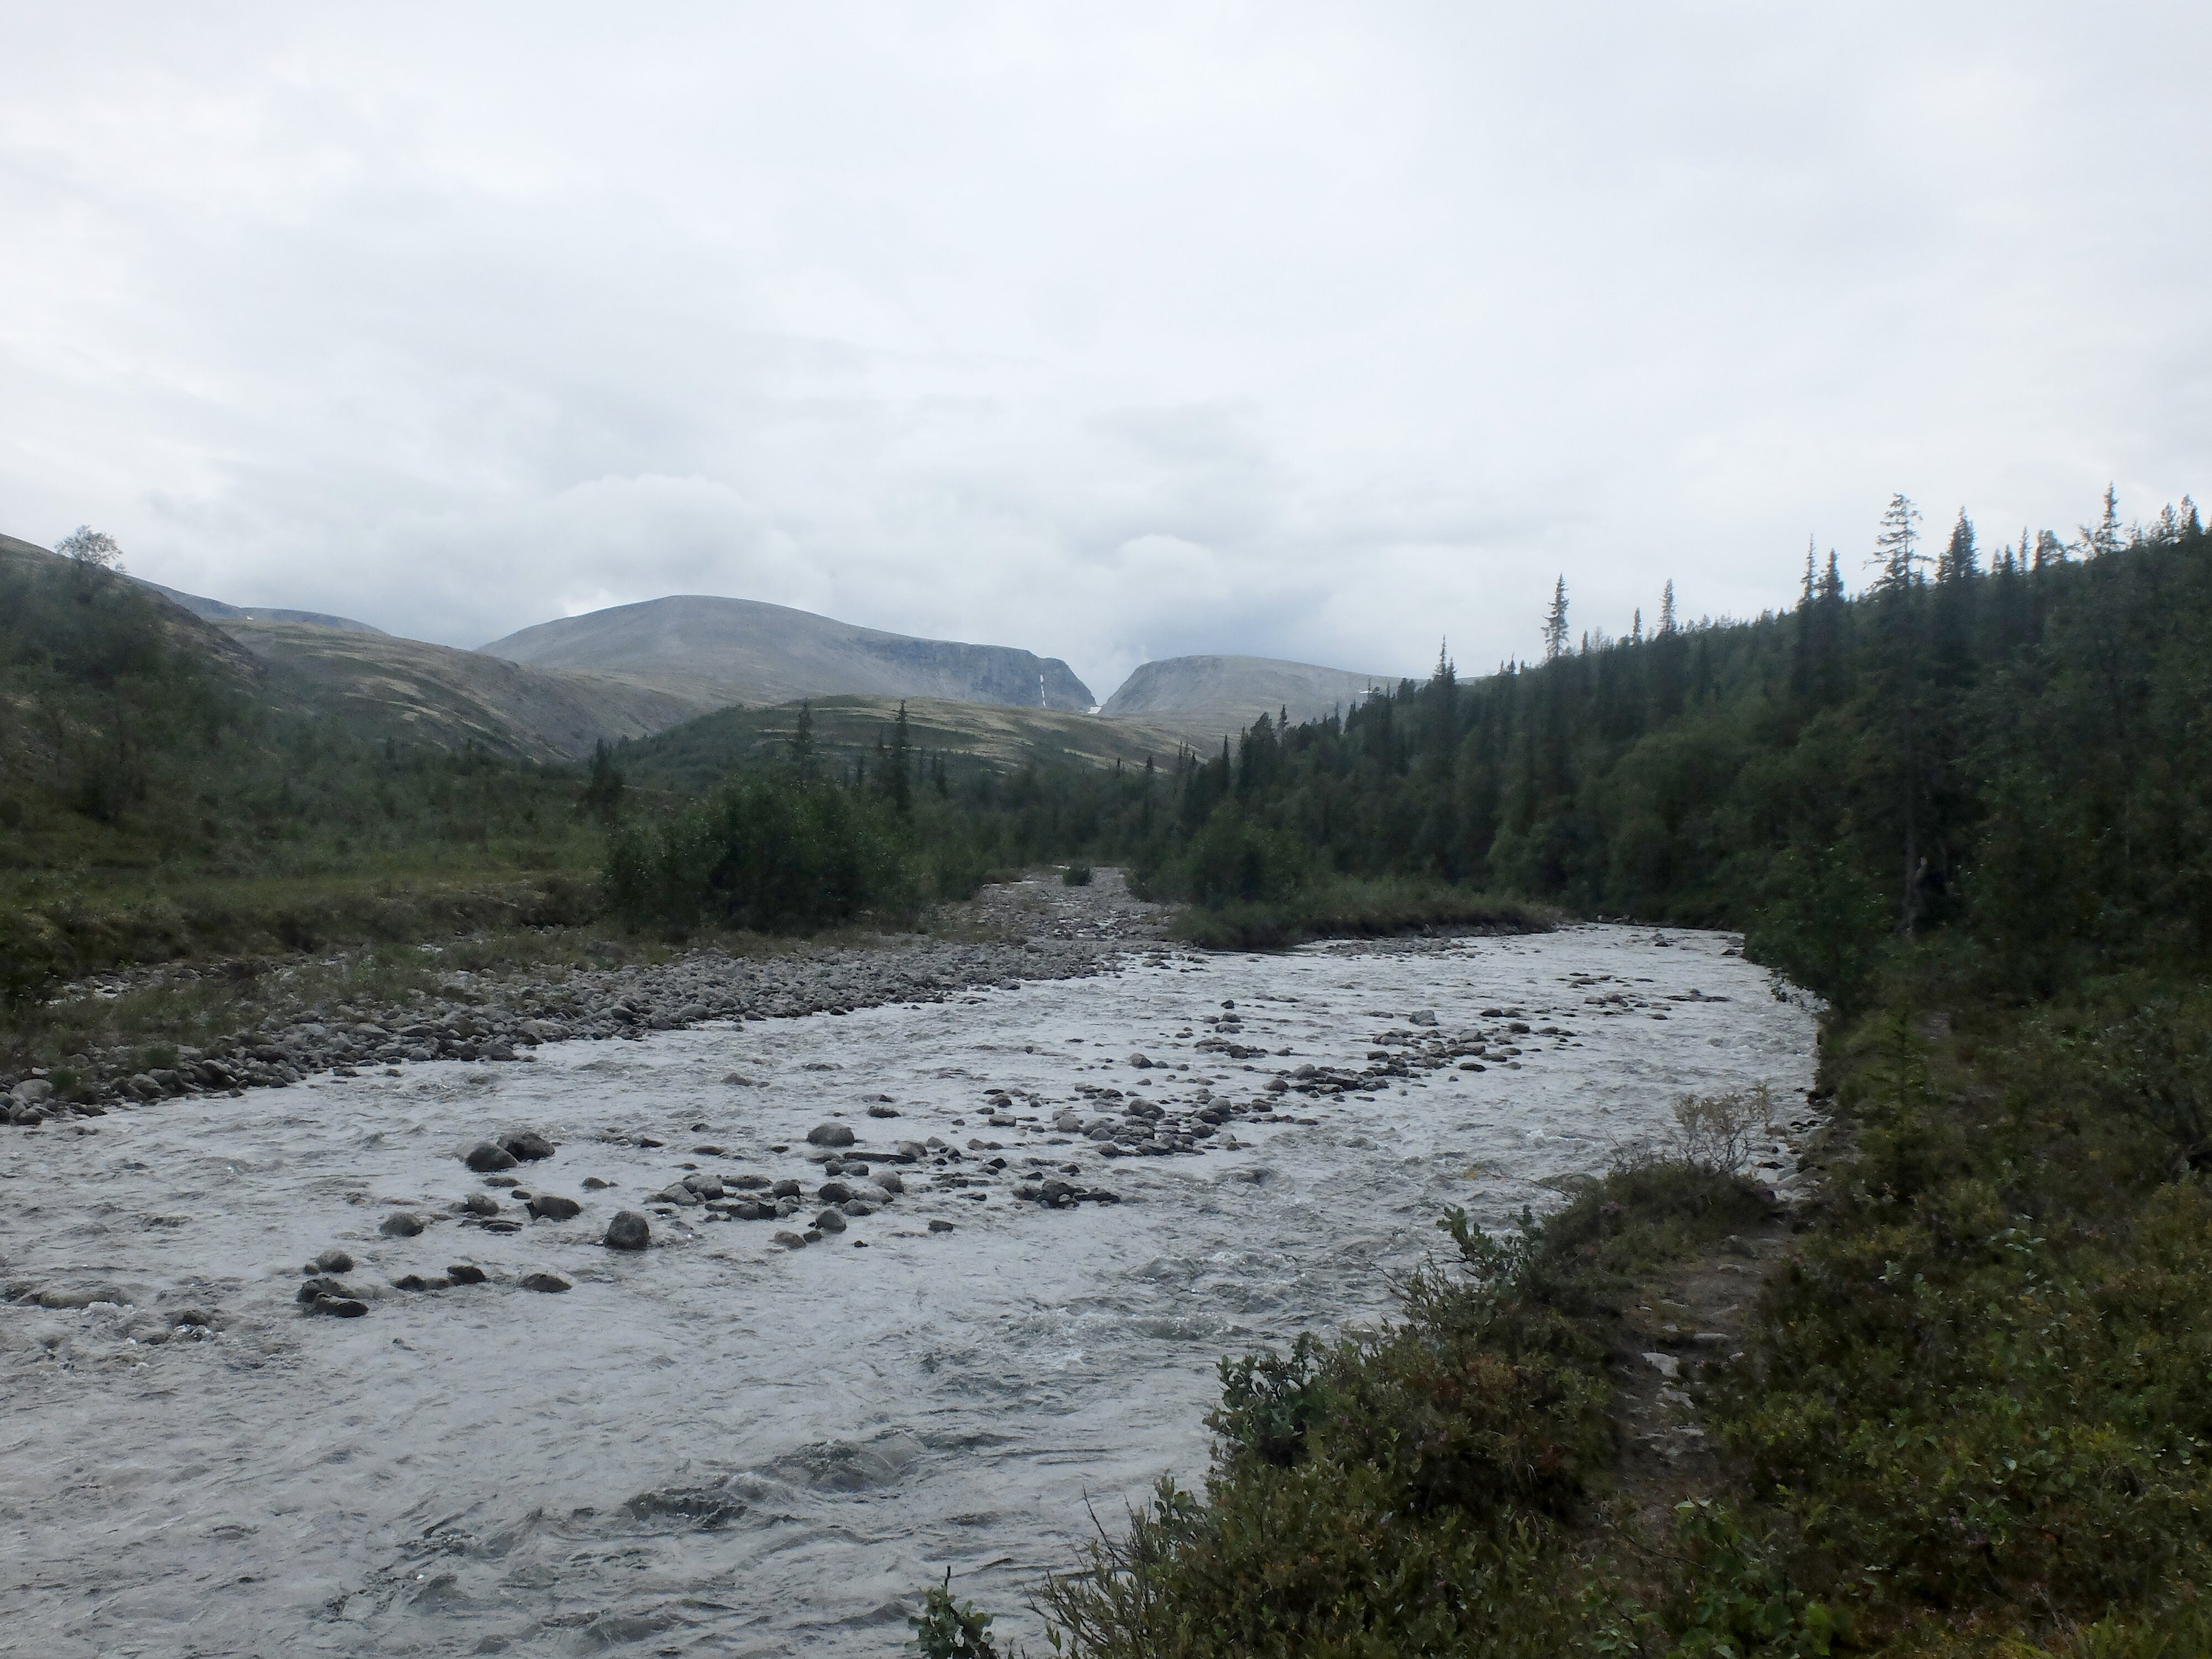
\includegraphics[width=14cm]{foto/10_08/01.Дорога вниз.png.jpg}
    \caption{Тропа вдоль р. Северный Каскаснюнйок. Вид назад}
    \label{fig6:2}
\end{figure}

\begin{figure}
    \centering
    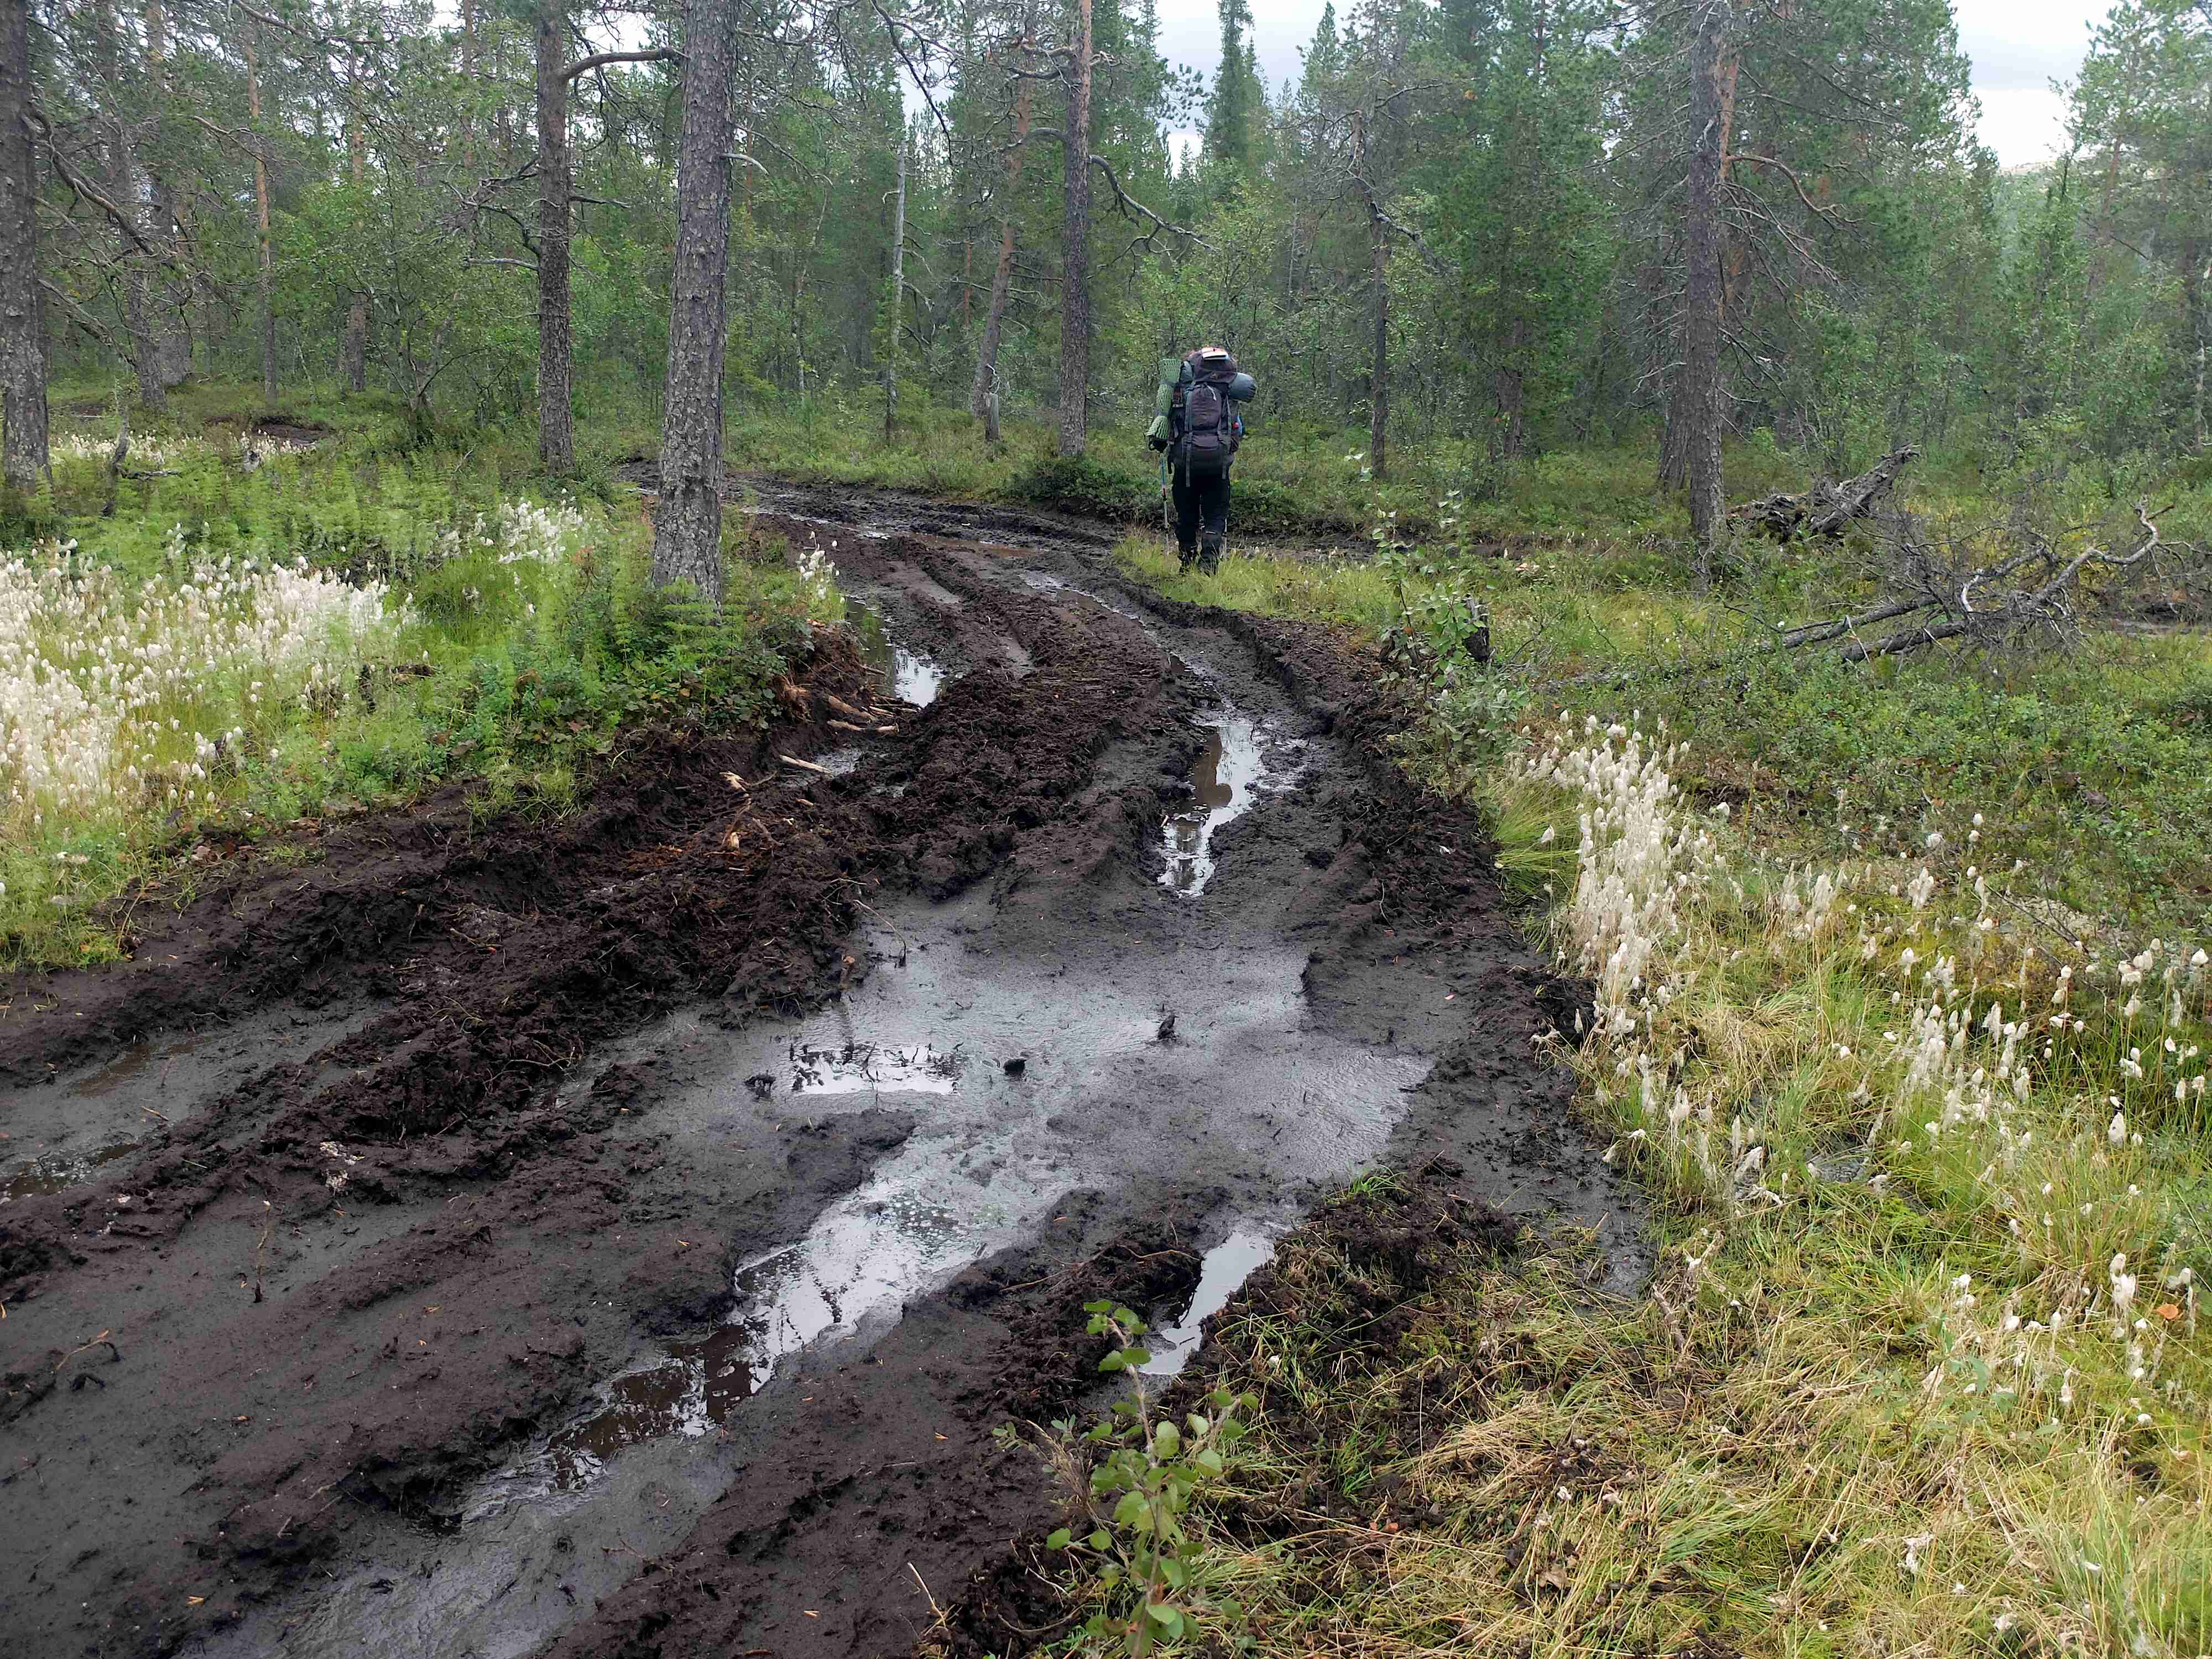
\includegraphics[width=14cm]{foto/10_08/03.Заболоченная дорога.png.jpg}
    \caption{Заболоченная дорога}
    \label{fig6:3}
\end{figure}

\begin{figure}
    \centering
    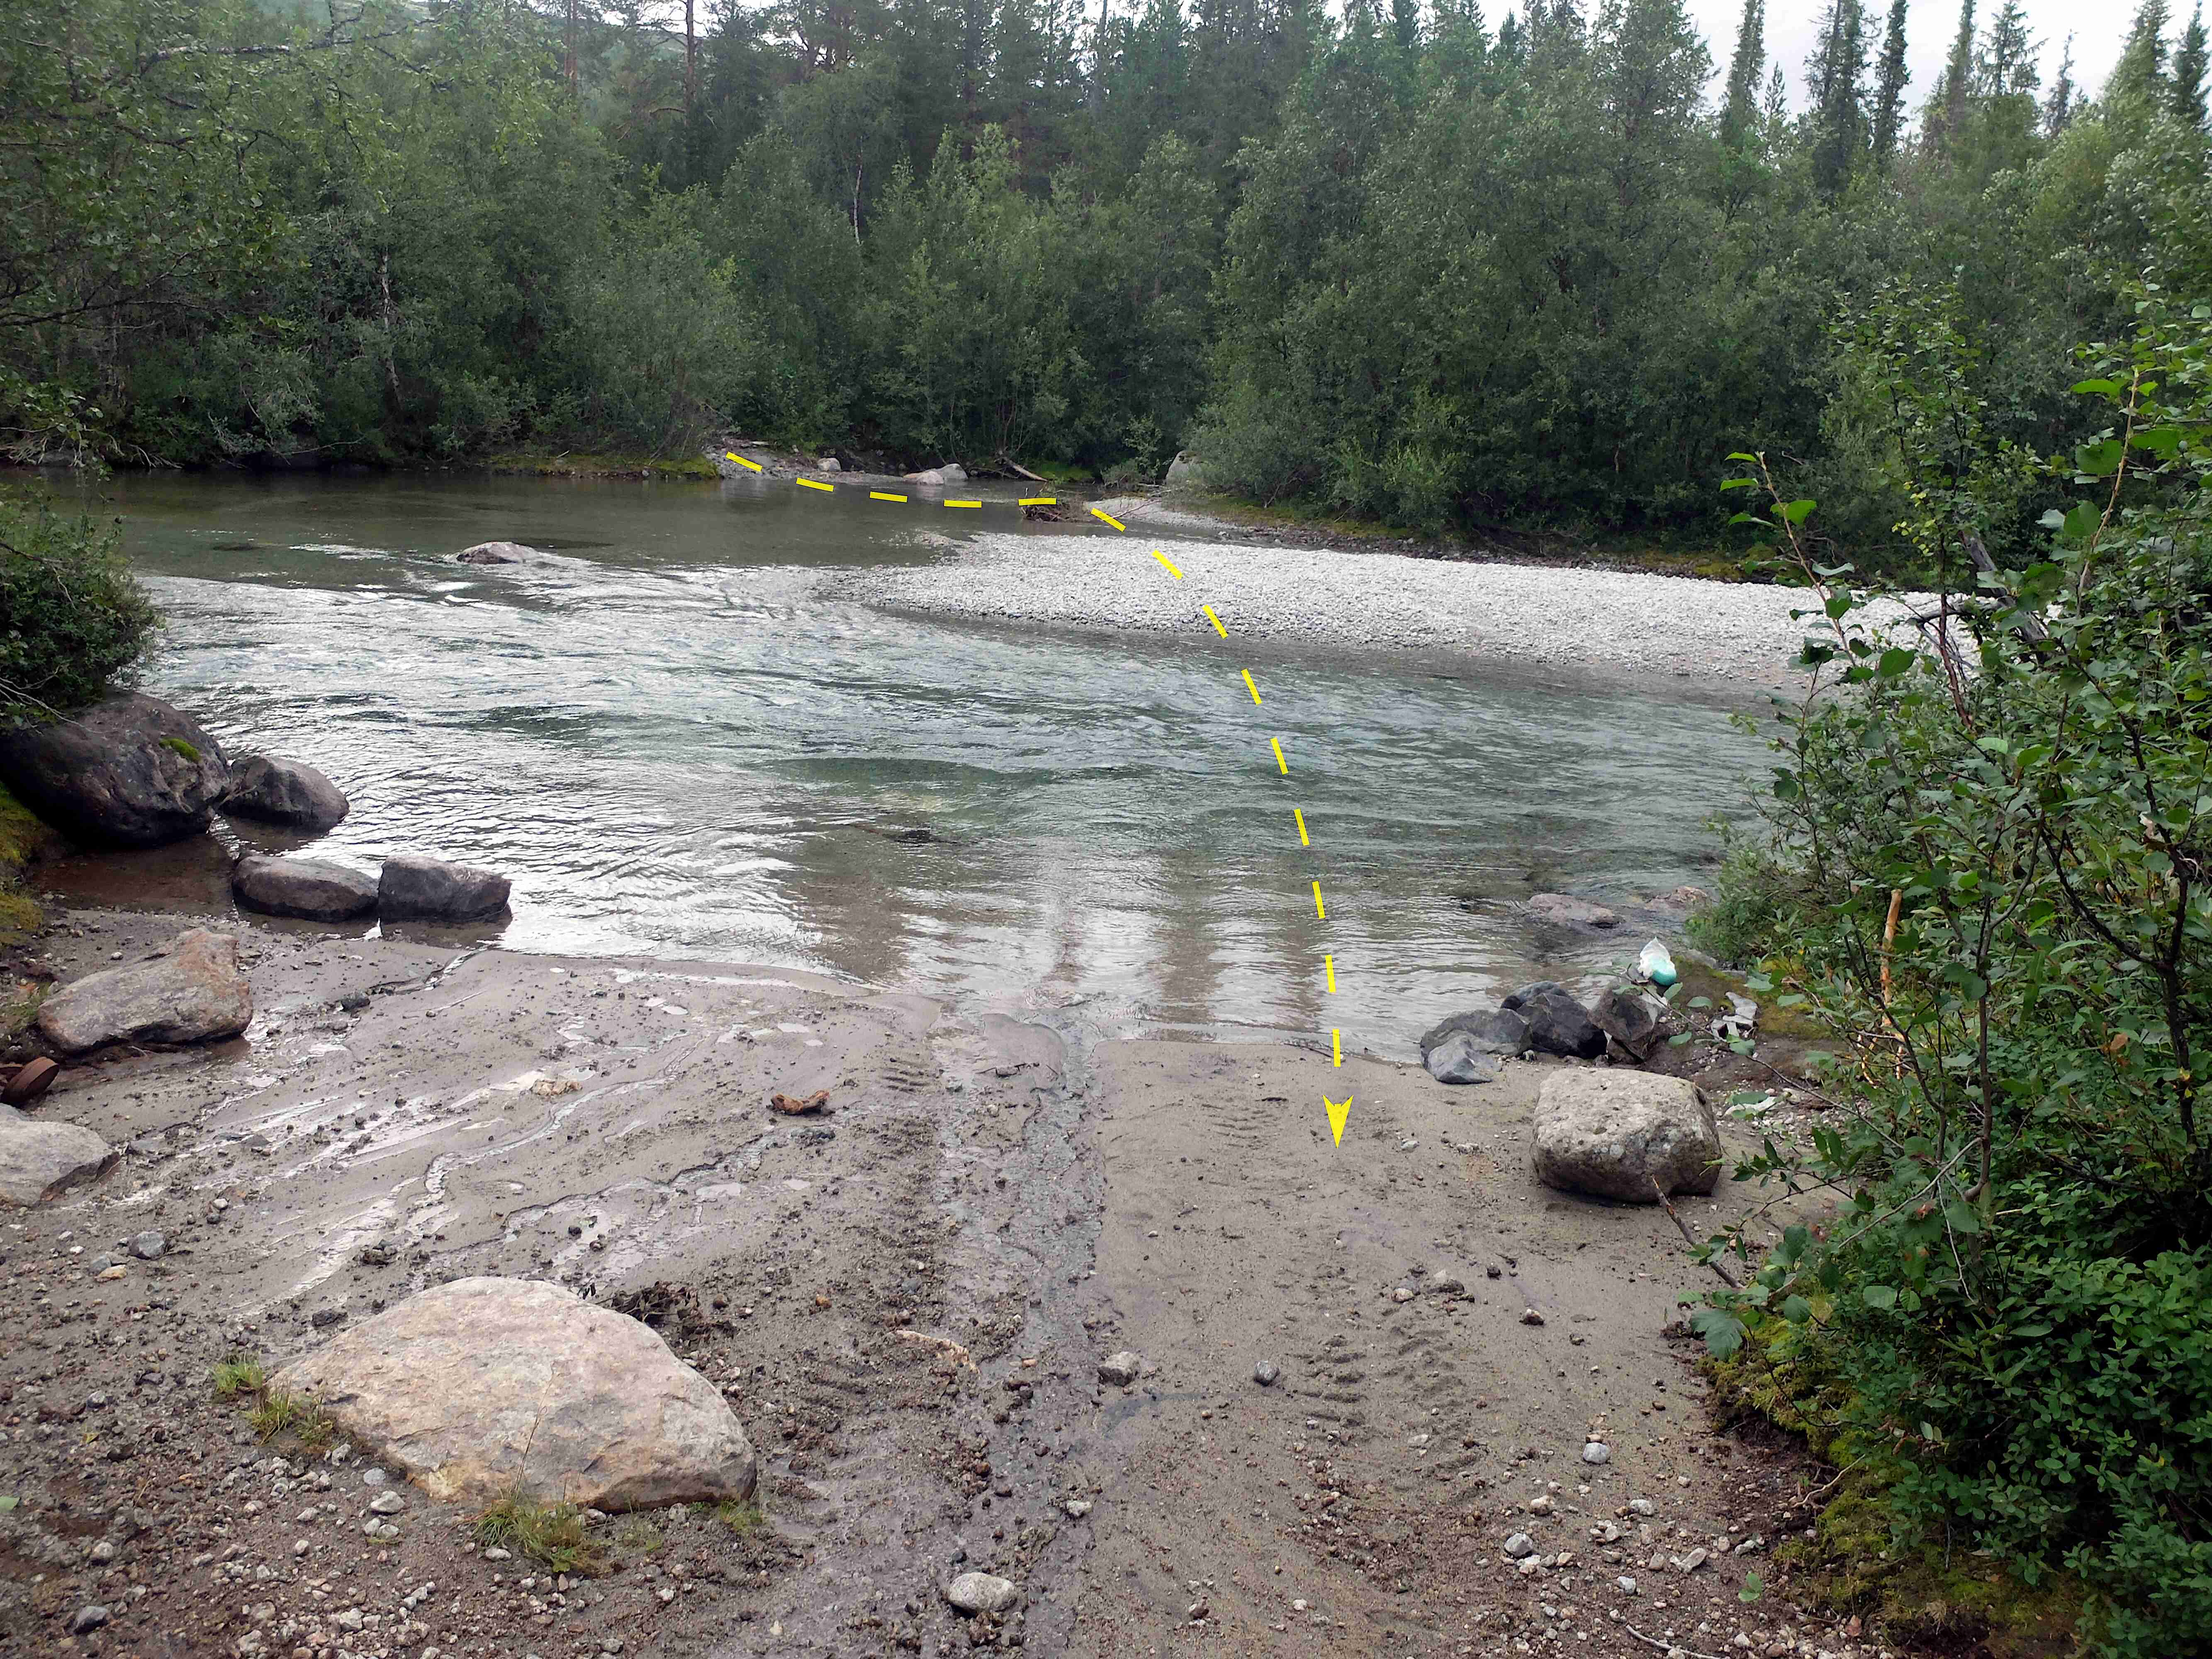
\includegraphics[width=14cm]{foto/10_08/04.Брод с юга.png.jpg}
    \caption{Вид на брод через р. Каскаснюнйок с юга}
    \label{fig6:4}
\end{figure}

\FloatBarrier

\subsection{День 7. 11.08.2022\\
Переправа р. Каскаснюнйок -- верш. Рыпнецк -- оз. Академическое}
\begin{tabular}{l p{12cm}}
\hline
Пройдено: & 14.77 км\\
Набор/сброс высоты: & 786/244 м\\
Время в пути: & 5:02\\
ЧХВ: & 4:08\\
Метеоусловия: & Утром --- дождь. Остаток дня --- переменная облачность.\\
\hline
\end{tabular}

Проспали, встали в 08:30, дождь.

11:10 Вышли.
Дорога идёт по гребню, потому из-за отсутствия ручьёв, гораздо лучше чем в предыдущий день.
Дорога вездеходная. Ветер, дождь, холодно. Показывается оз. Умбозеро. Пока есть связь звоним в МЧС, и смс координатору.

Незадолго до верш. Рыпнецк заканчивается дождь, начинает проглядывать солнце (рис. \ref{fig7:1}).
Отличные обзорные виды на окрестные горы (рис. \ref{fig7:2}),
можно делать панораму. На Рыпнецке записка \enquote{двух влюблённых} (парочки прошедшей днём ранее) (рис. \ref{fig:zapiski4}),
не снимаем.

После вершины небольшой спуск (130 метров) в седловину пер. Куропачий (н/к) (рис. \ref{fig7:3}), затем снова подъём почти
до самого оз. Академического.

У озера сильный ветер. Встречаем снимающих лагерь \enquote{влюблённых}, они от ветра  встали за гребнем, вдали от озера.
У самого озера несколько площадок, в разной степени защищённых стенами из камней.
Выбираем самую закрытую площадку, ставимся (рис. \ref{fig7:4}--\ref{fig7:5}). Немного достраиваем стену. Обедаем, потом сон до 21.

21:00 Ужин.

23:00 Отбой. Облачно с прояснениями, луна, непрекращающийся ветер, +13$\tccentigrade$.

\begin{figure}
    \centering
    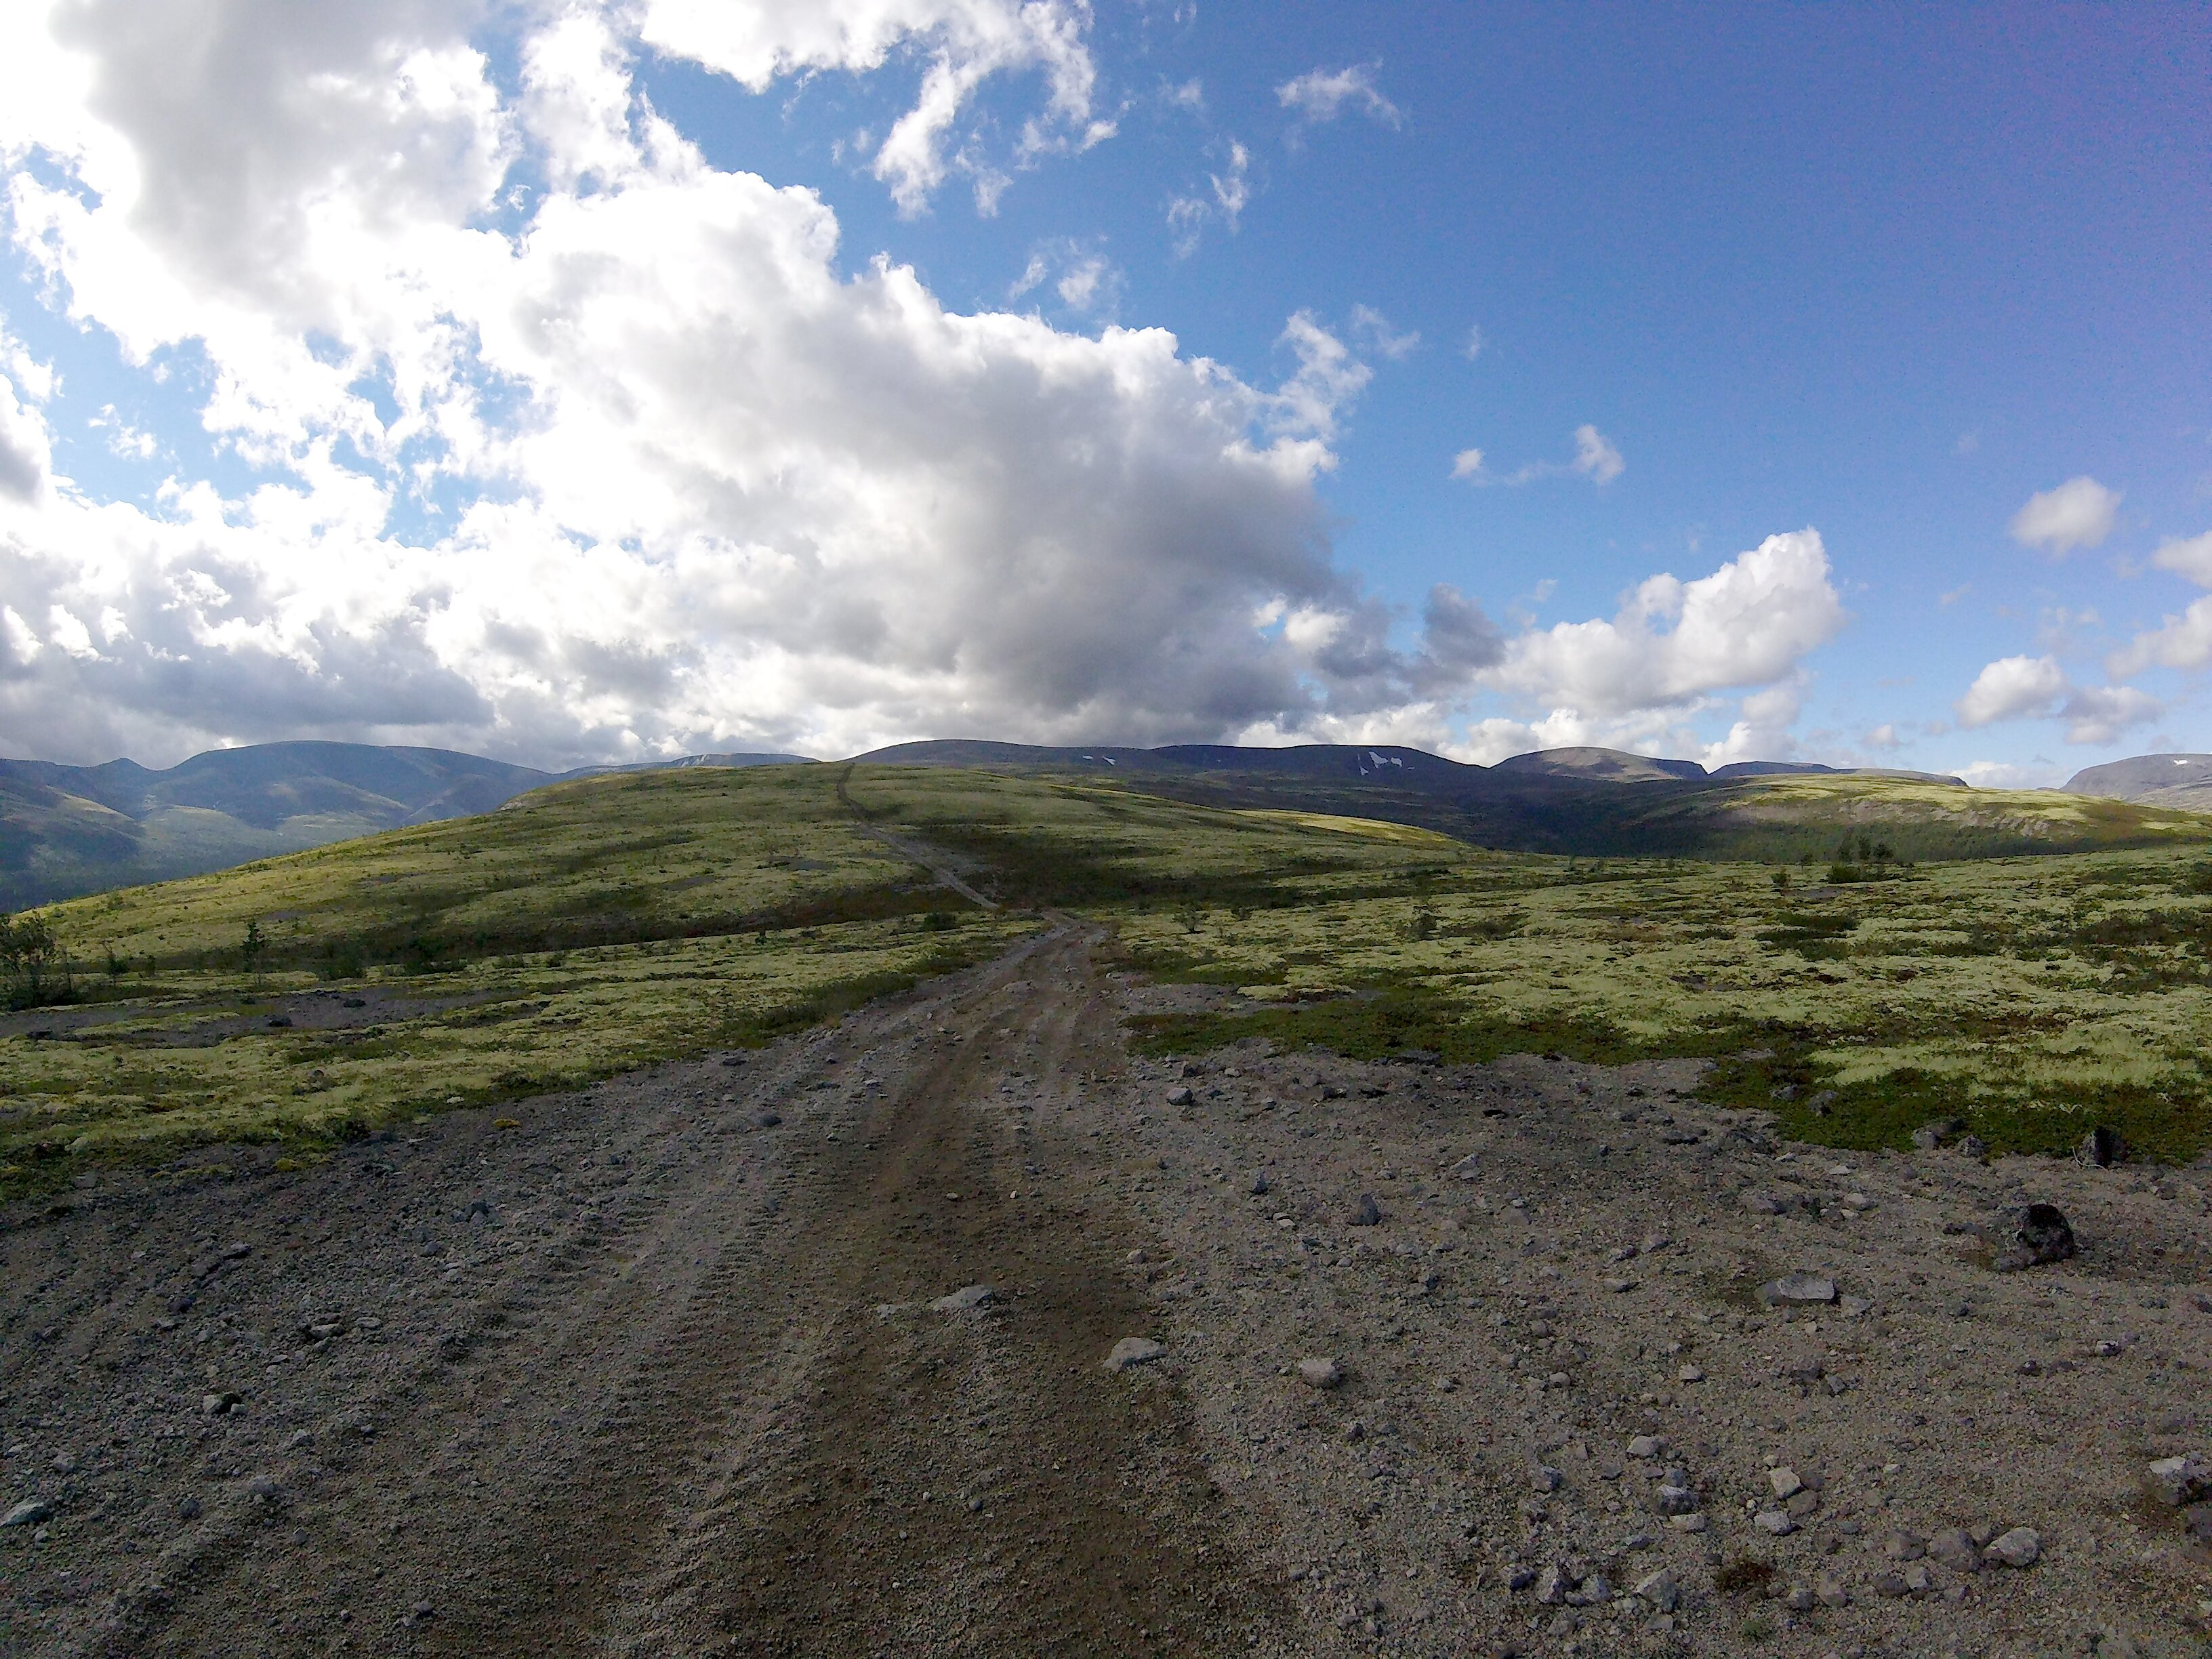
\includegraphics[width=14cm]{foto/11_08/01.Дорога к верш. Рыпнецк.png.jpg}
    \caption{Дорога к верш. Рыпнецк}
    \label{fig7:1}
\end{figure}

\begin{figure}
    \centering
    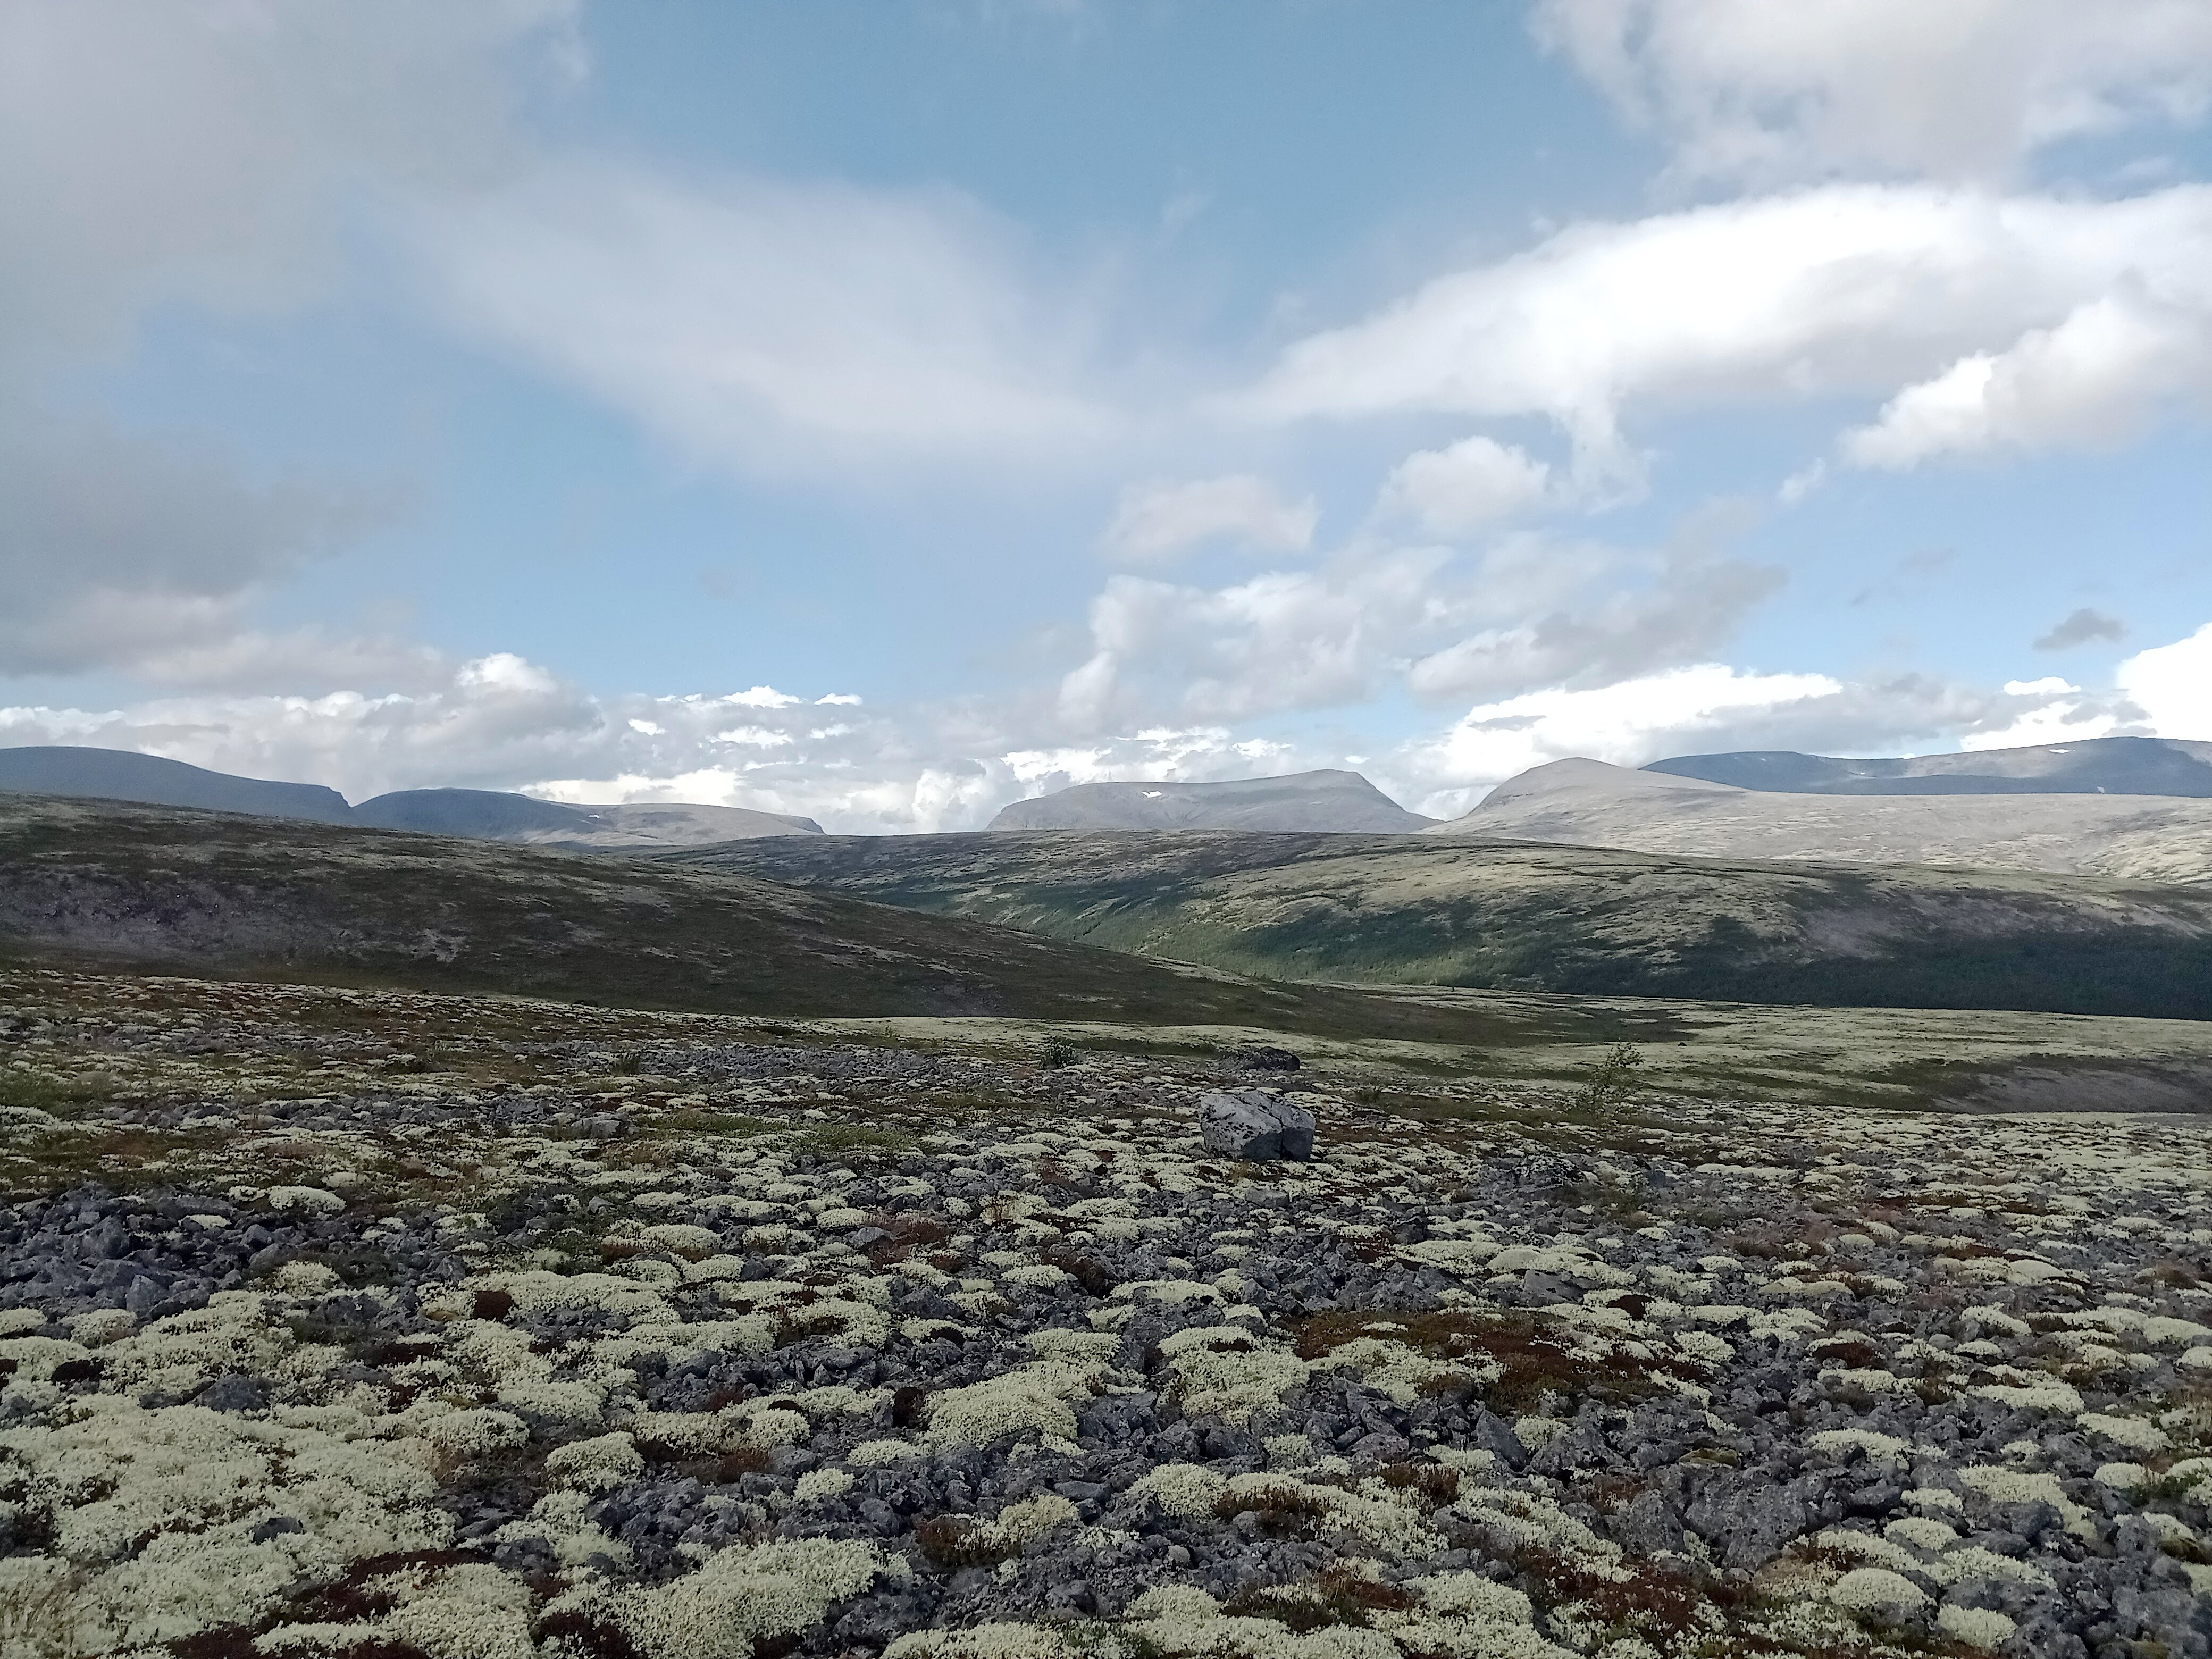
\includegraphics[width=14cm]{foto/11_08/02.Вид на север перевалы.png.jpg}
    \caption{Вид на перевалы на севере}
    \label{fig7:2}
\end{figure}

\begin{figure}
    \centering
    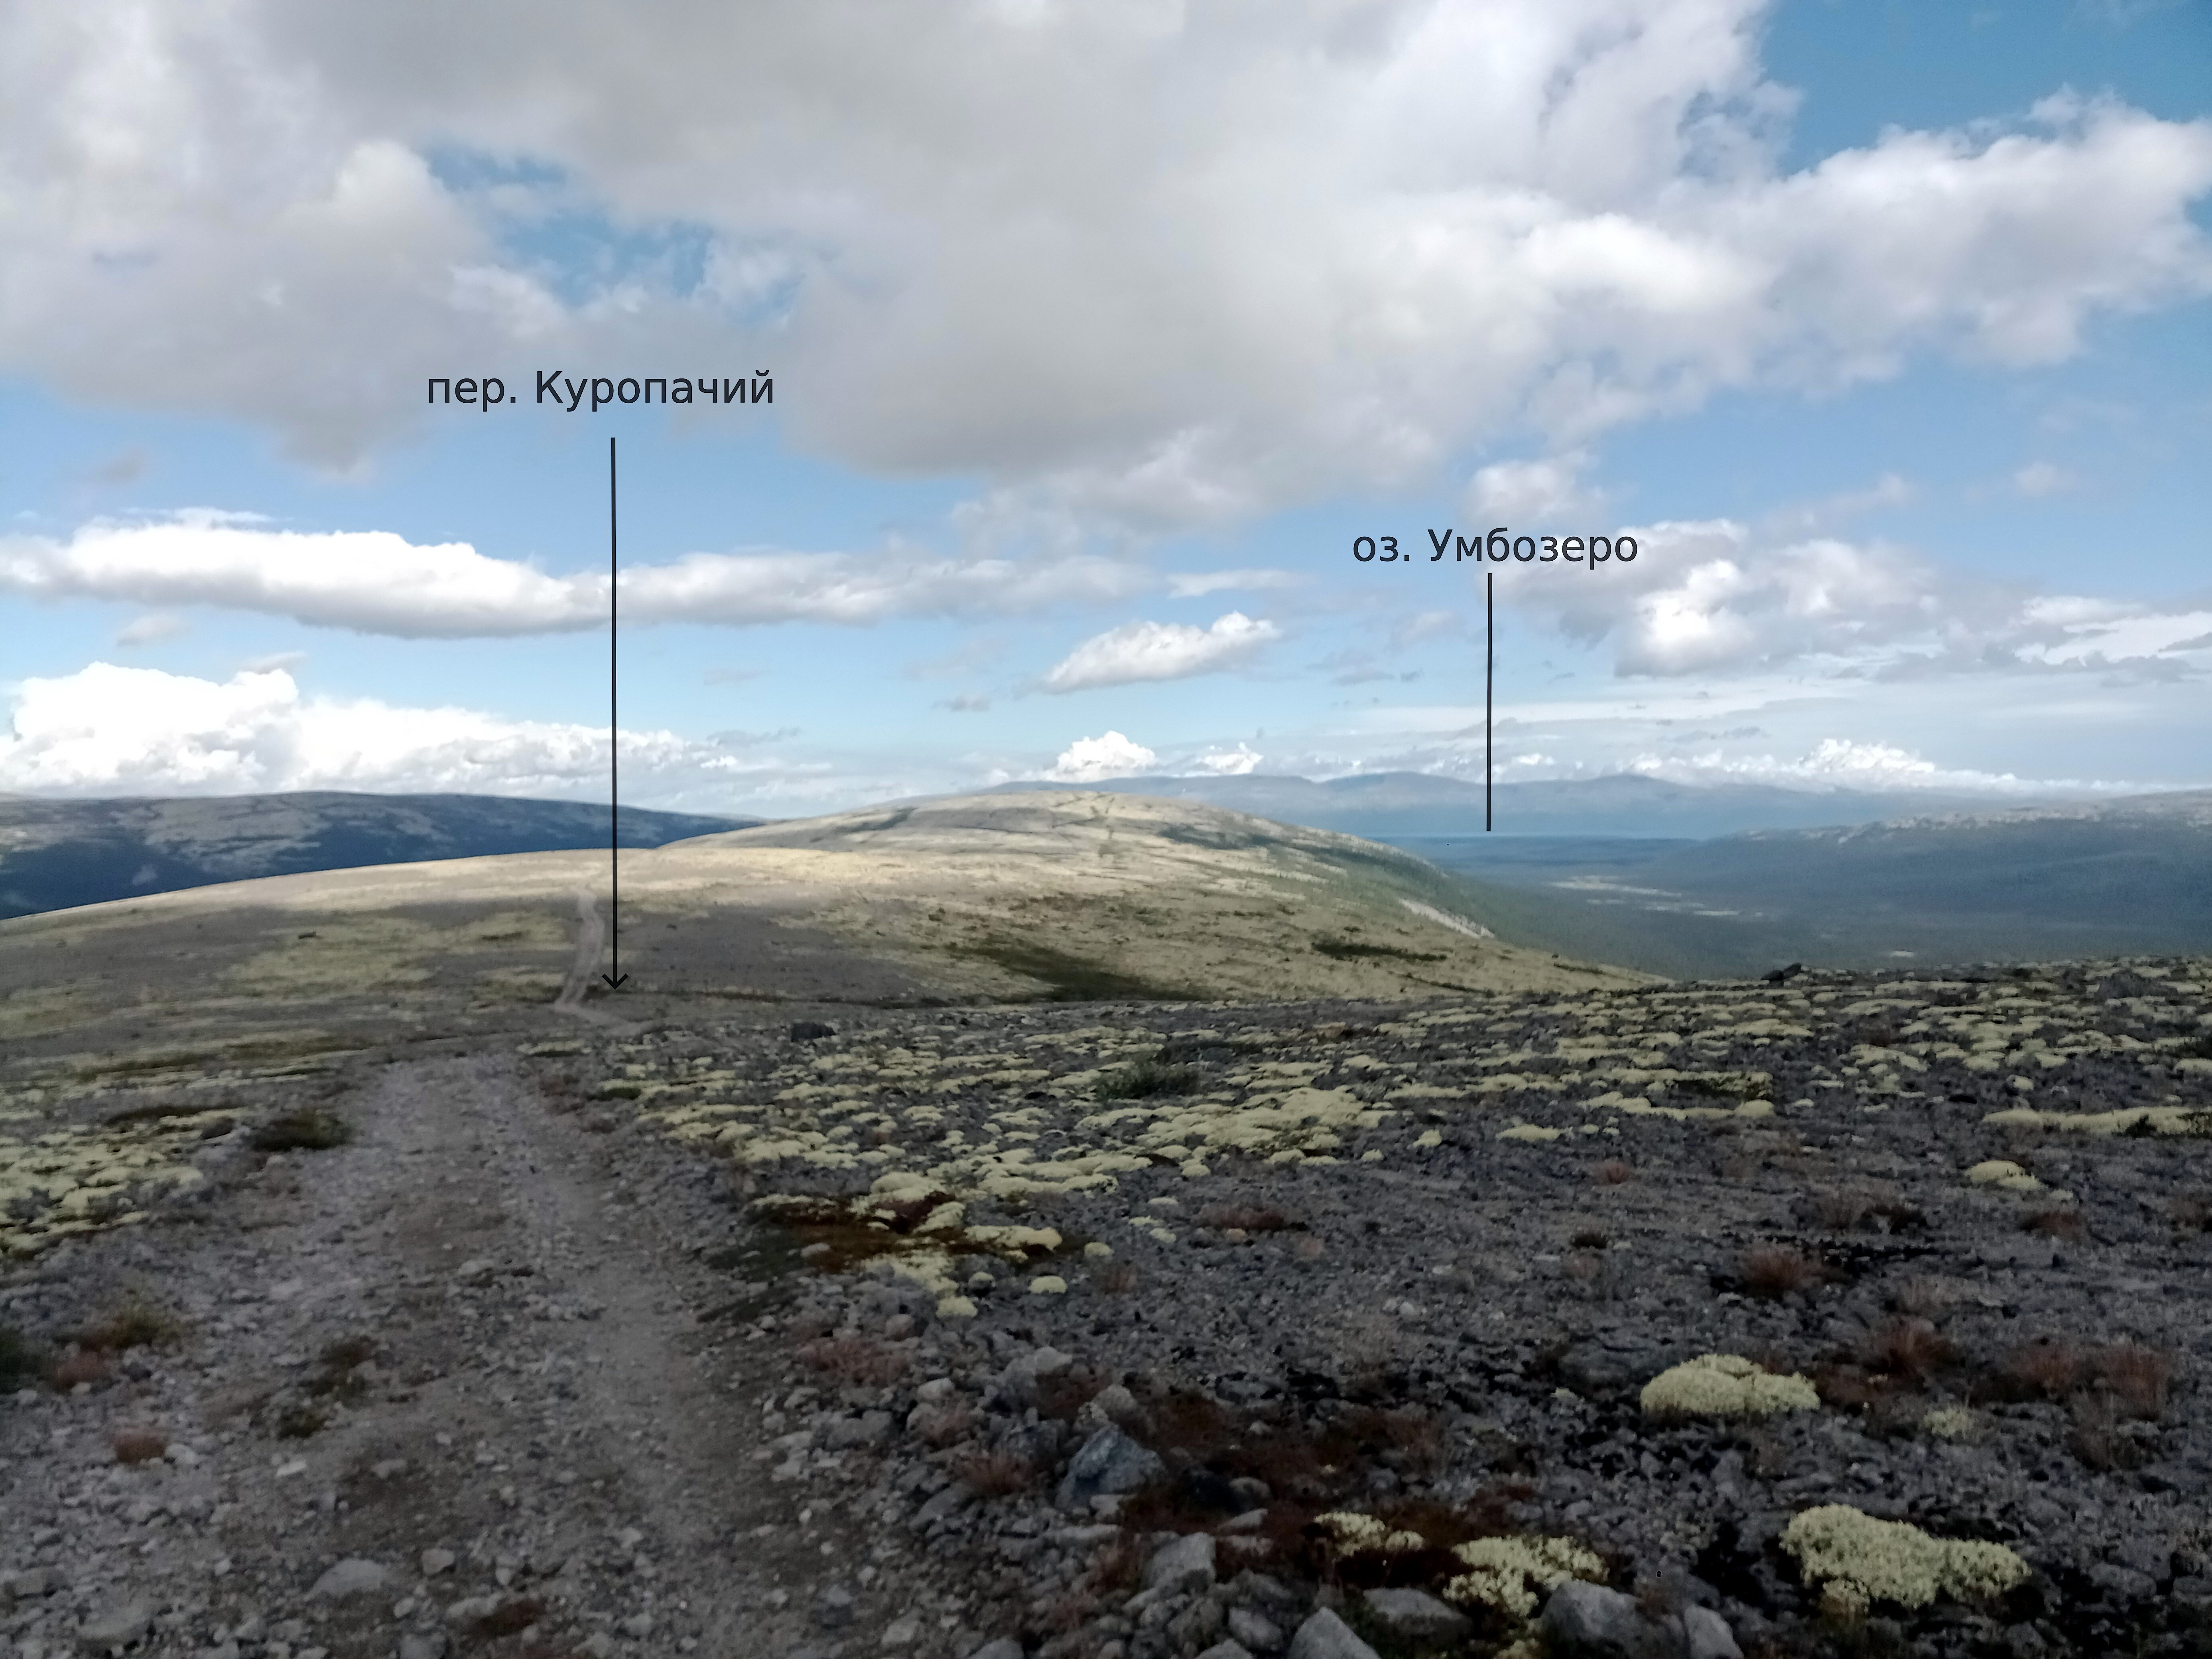
\includegraphics[width=14cm]{foto/11_08/03.Вид на перевал Куропачий с дороги к оз. Академическому.png.jpg}
    \caption{Вид на пер. Куропачий. Взгляд назад}
    \label{fig7:3}
\end{figure}

\begin{figure}
    \centering
    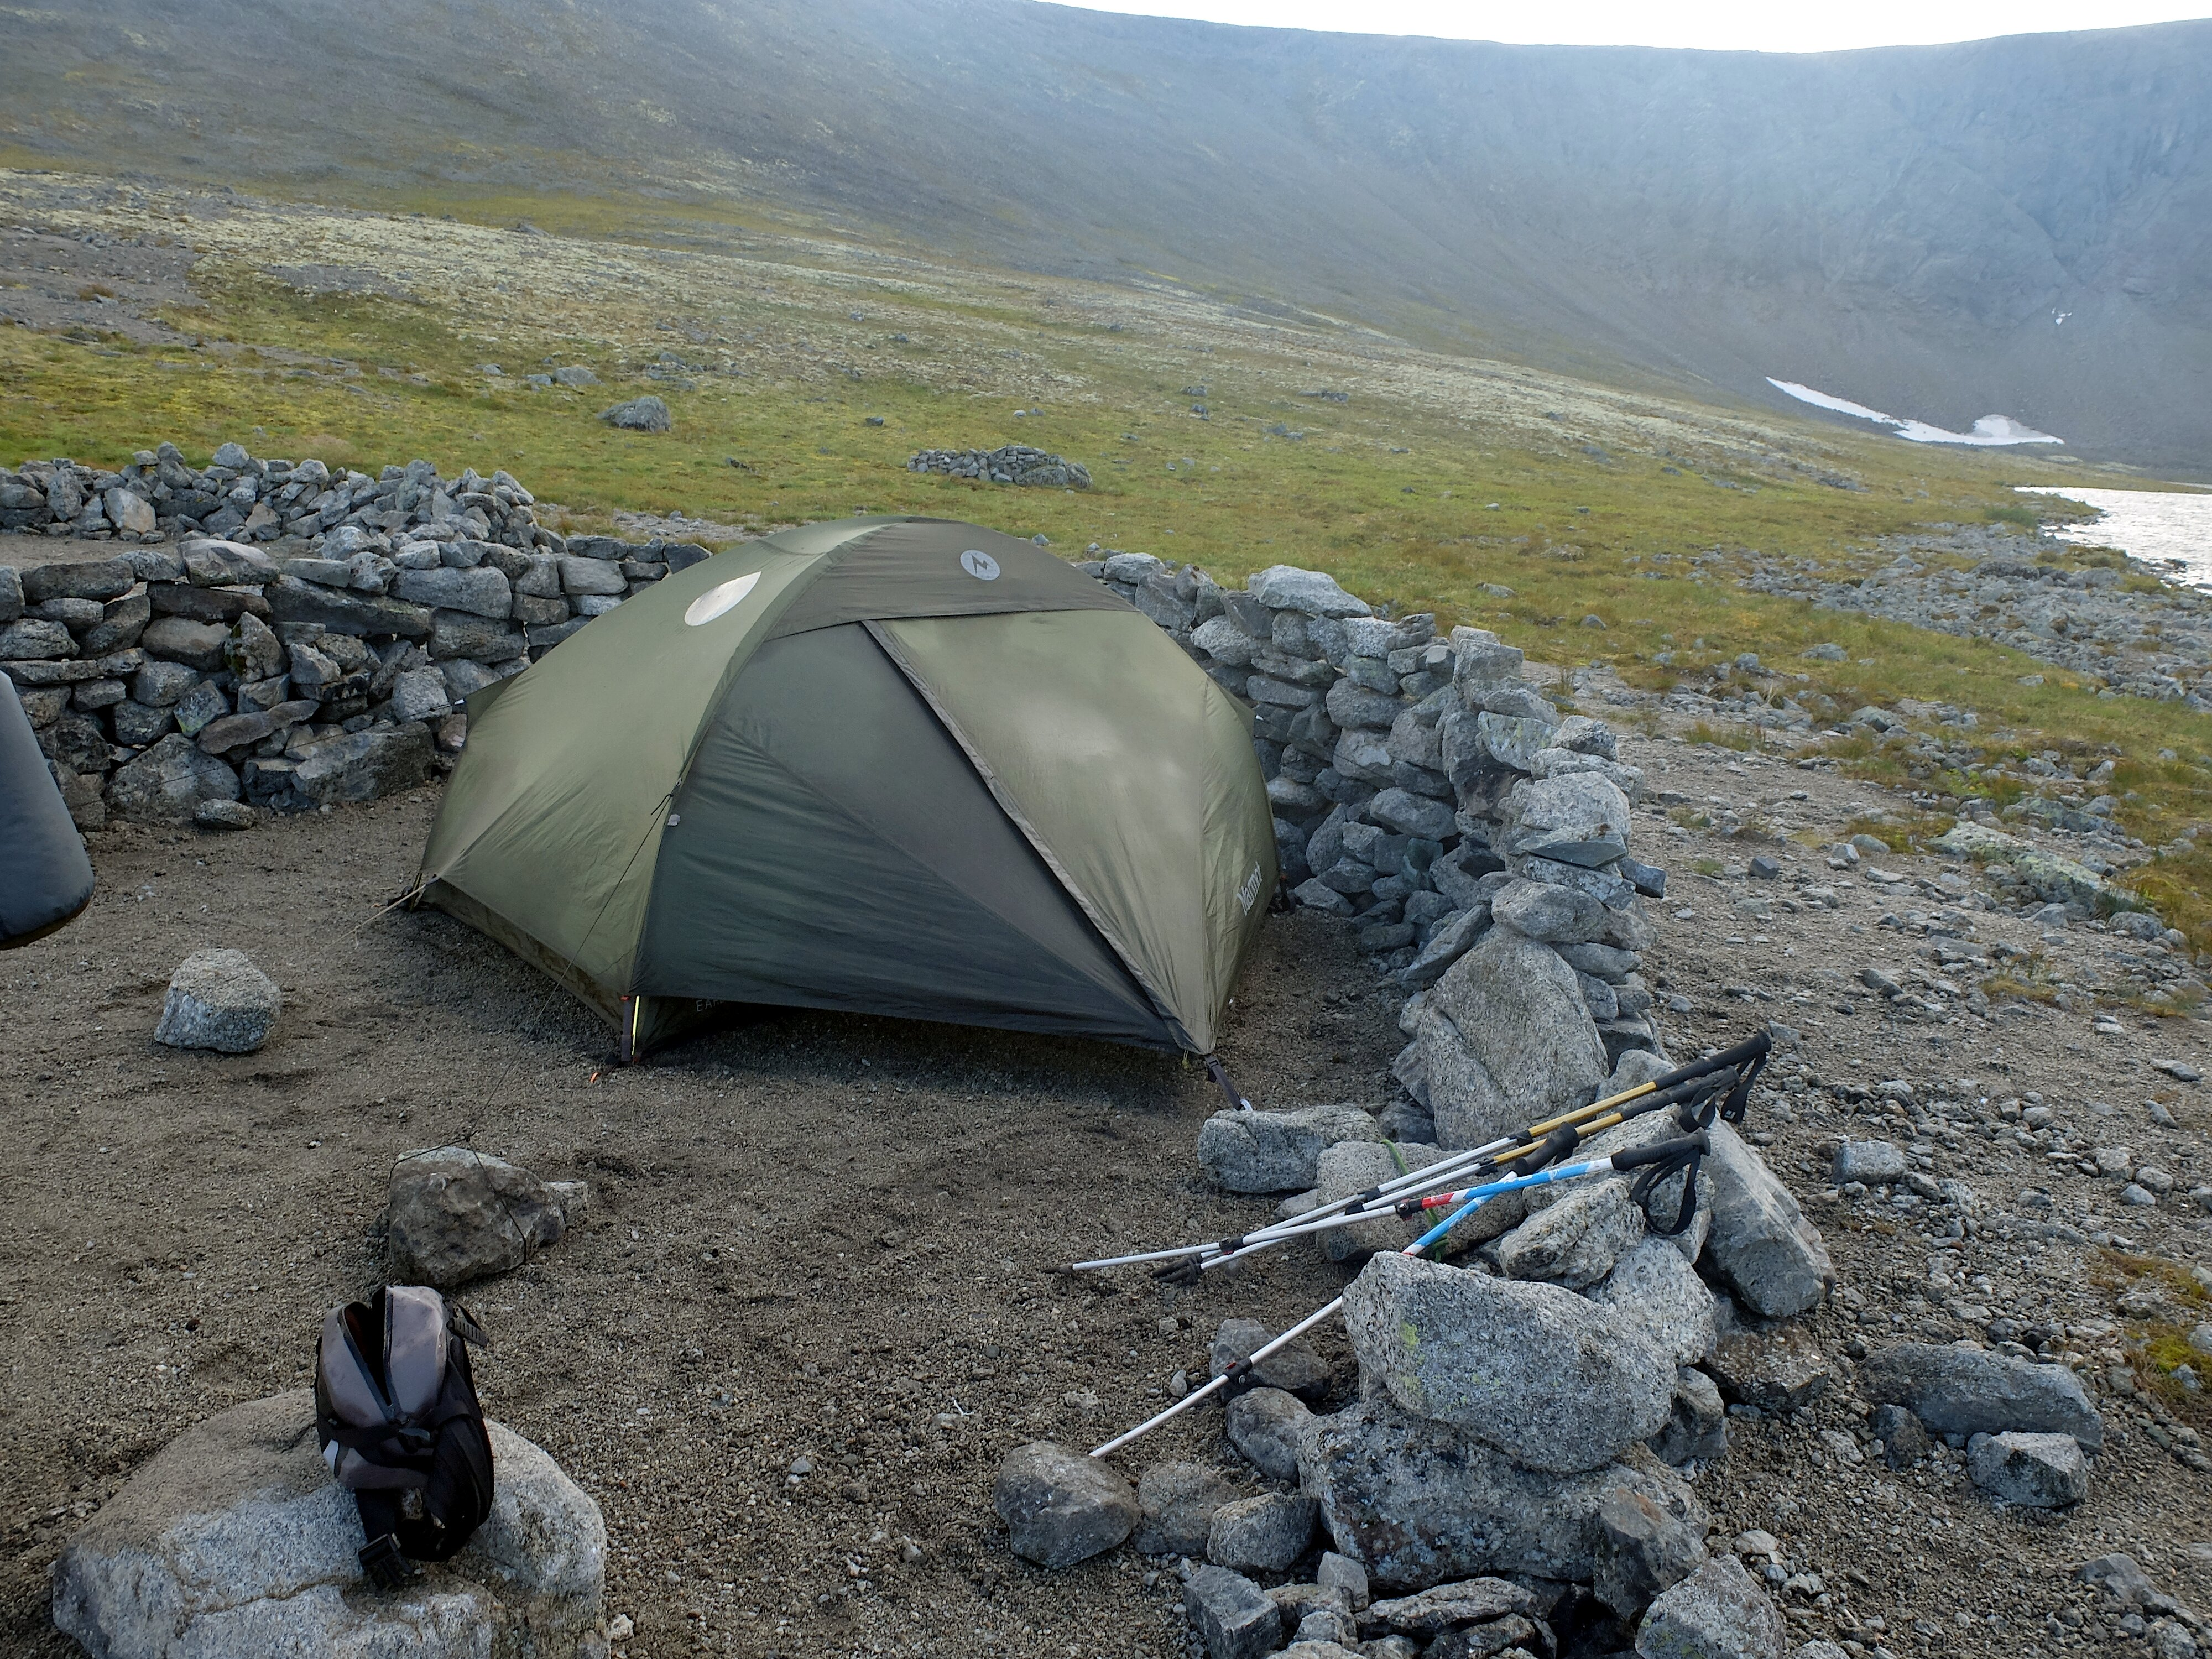
\includegraphics[width=14cm]{foto/11_08/04.Стоянка у оз. Академическое.png.jpg}
    \caption{Стоянка у оз. Академическое}
    \label{fig7:4}
\end{figure}

\begin{figure}
    \centering
    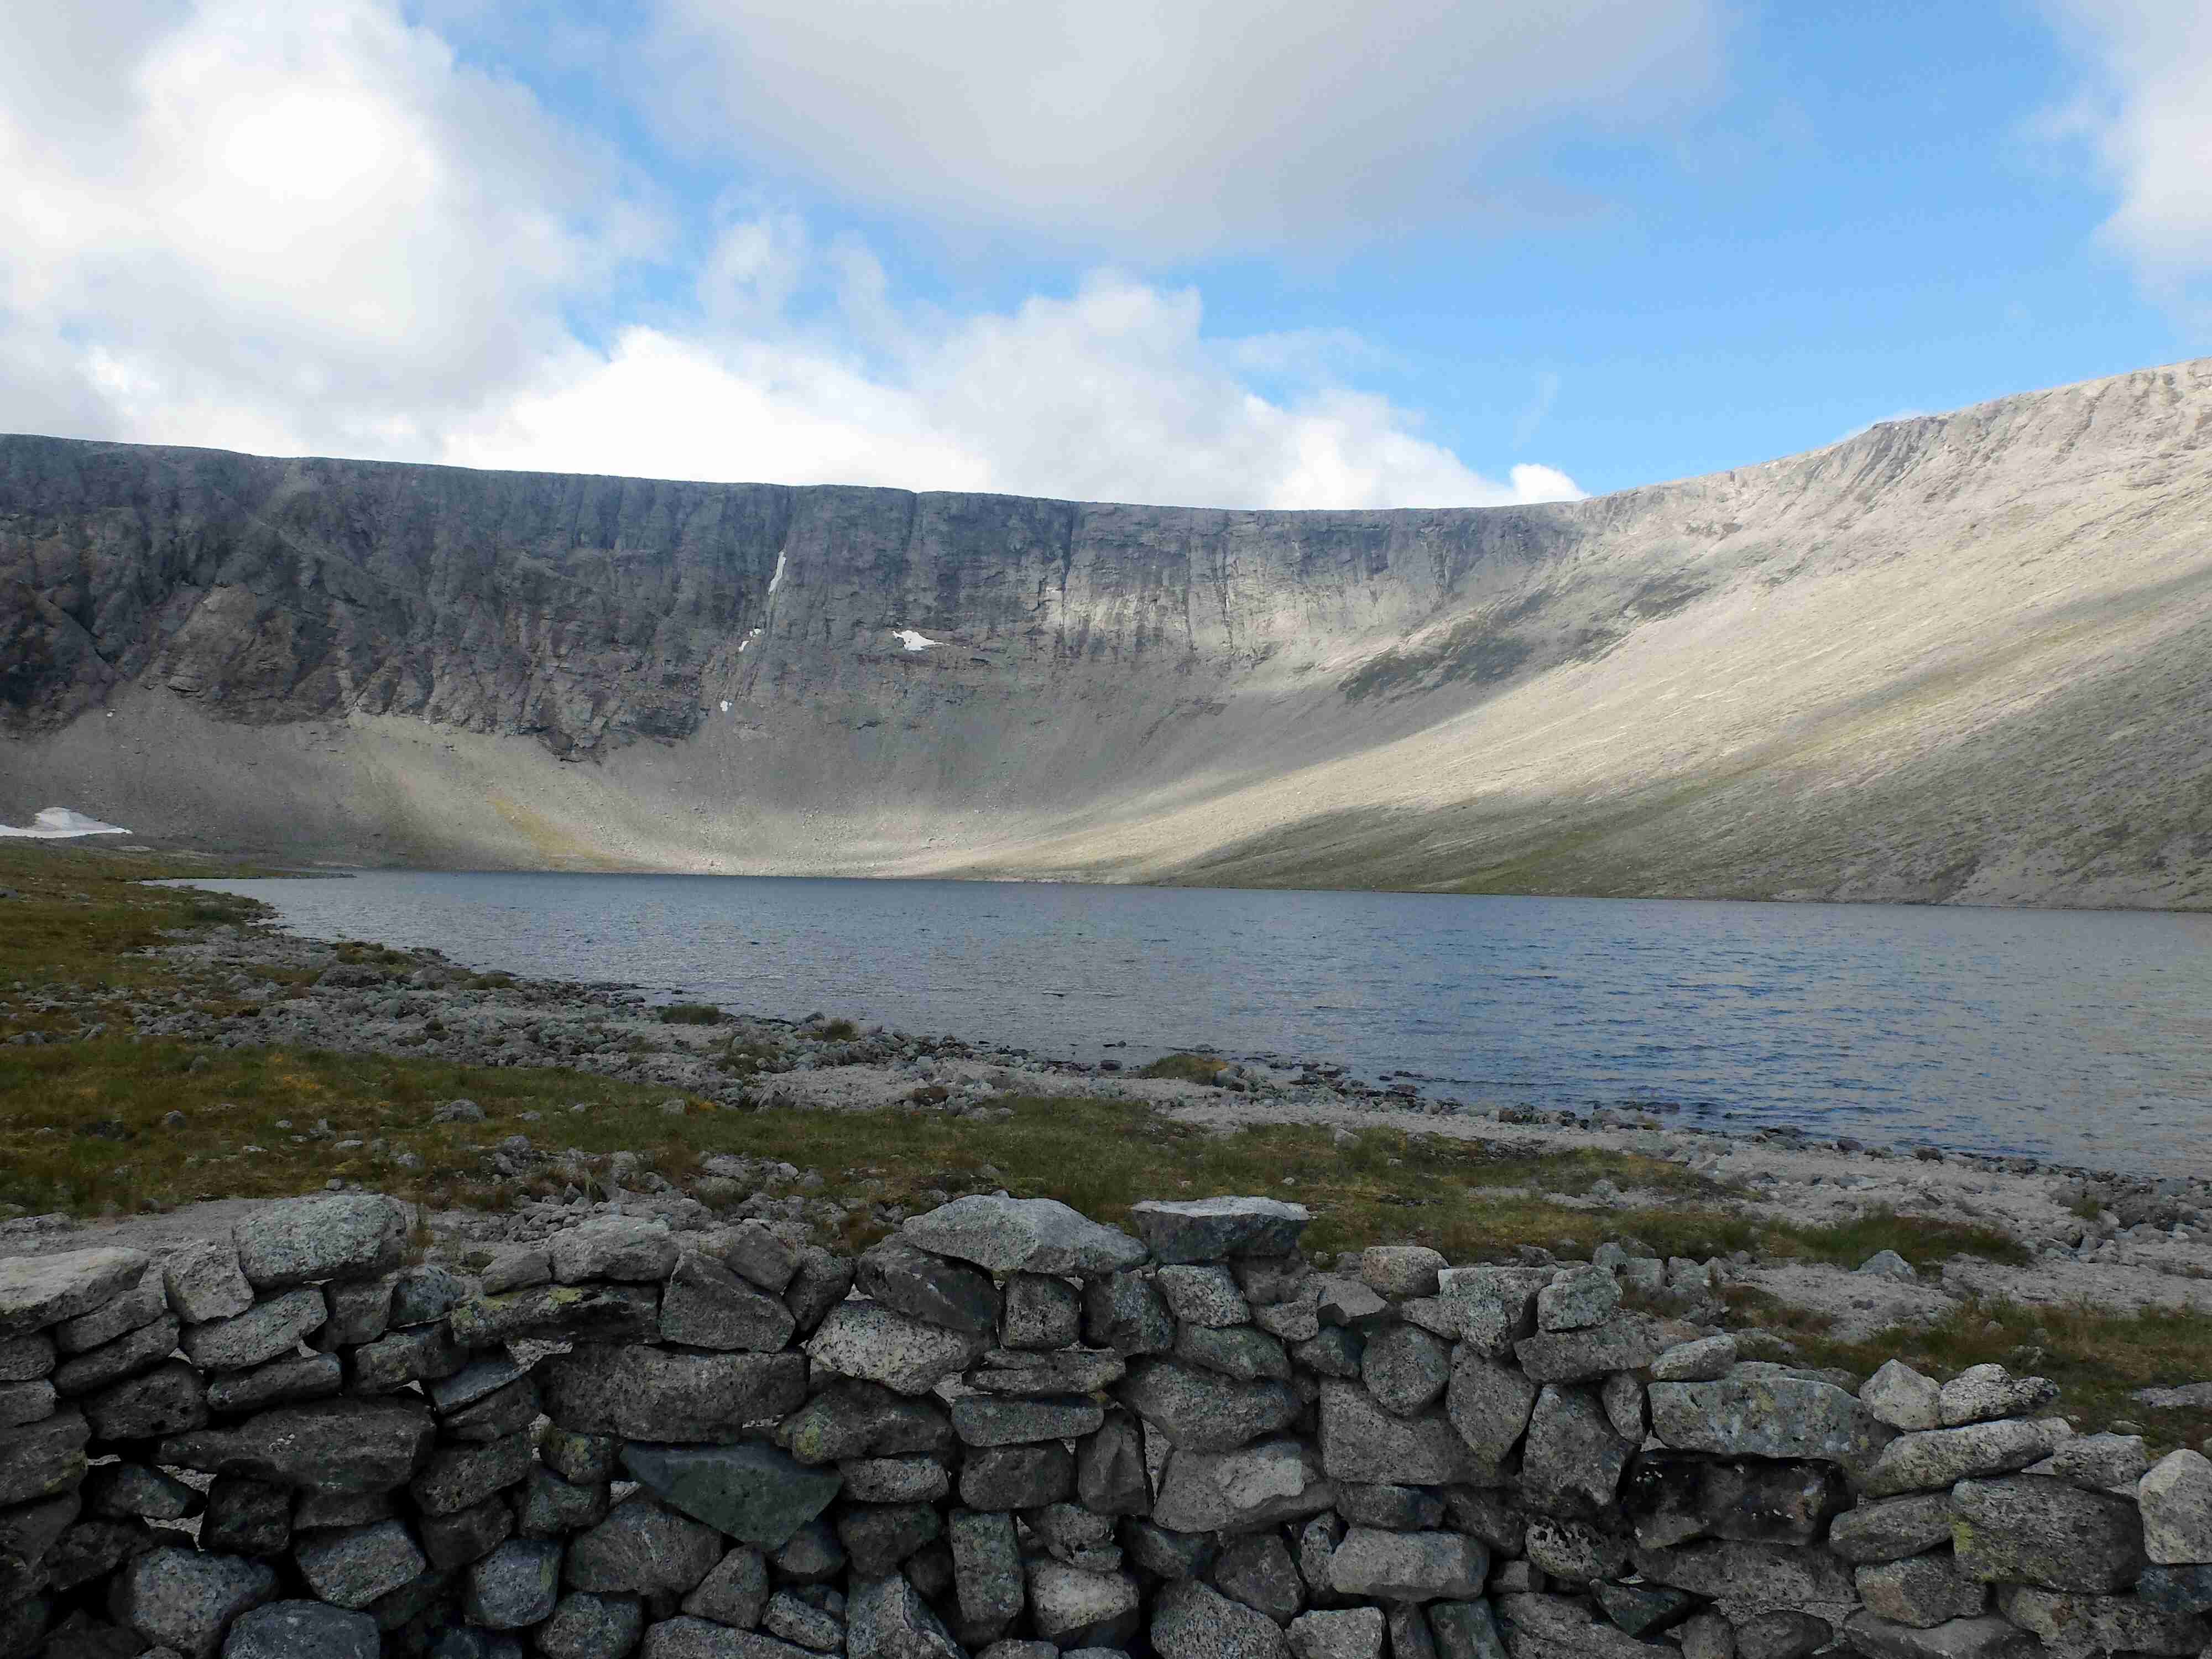
\includegraphics[width=14cm]{foto/11_08/05.Озеро Академическое.png.jpg}
    \caption{Оз. Академическое}
    \label{fig7:5}
\end{figure}

\FloatBarrier

\subsection{День 8. 12.08.2022\\
Оз. Академическое -- пер. Исток (н/к, 1075, траверс) -- р. Вудьяврйок -- оз. Малый Вудъявр}
\begin{tabular}{l p{12cm}}
\hline
Пройдено: & 13.85 км\\
Набор/сброс высоты: & 454/861 м\\
Время в пути: & 5:33\\
ЧХВ: & 4:48\\
Метеоусловия: & Переменная облачность, временами дождь.\\
\hline
\end{tabular}

08:30 Подъём. Светит солнце, на горизонте тучи, +19$\tccentigrade$.
За каменной стенкой от ветра спали нормально, в палатке ночью было до +10$\tccentigrade$.

10:51 Выходим. Идём вверх по дороге, в сторону перевала Исток (н/к, 1075, траверсом), идётся нормально (рис. \ref{fig8:1}).
Сверху открывается вид на Академическое (рис. \ref{fig8:2}).
Нагнал дождь. Вообще весь день погода была переменная: то поливало, то выглядывало солнце.

Поворачиваем по дороге налево. Небольшой спуск по дороге в седловину пер. Исток 12:28.
Сфотографировали записку группы туристов из Петербурга (ДЮЦ Петергоф) под руководством Чеснокова Д.В. от 06.08.2022
(рис. \ref{fig:zapiski5}),
забирать не стали поскольку перевал шли траверсом. Здесь же встретили бегуна, бежал снизу от цивилизации к оз. Академическому.

Далее пологий подъём к вершине Кукисвумчорр.
13:00 Вершина, геодезический знак. Турик был пустой, само место замусорено.

К вершине подошли азимутом, автодорога ушла правее. Попытались пойти дальше по турикам, но они, видимо,
были беспорядочно наставлены любителями собирать камни, тропу не указывают. В конце концов пошли на запад
в сторону дороги пока не нашли её. Когда дорога кончилась, пошли азимутом к створу склона (рис. \ref{fig8:3}).
Створ склона образован сужающимися справа и слева обрывами. Основная опасность там, кажется, внезапные порывы ветра,
поэтому близко к краям обрыва без страховки подходить не стоит. После начинается понятная тропа на спуск.
Вначале идёт крутой курумник со средними камнями (рис. \ref{fig8:4}--\ref{fig8:5}).
Далее несколько чередующихся участков спуск-плато меньшей крутизны.
В итоге мы спустились по гребню до ручья по левую руку, а далее тропами по обеим сторонам ручья.
Как вариант (из 2015 года) --- спуститься по склону вправо, сразу к центральной автодороге от КСС до оз. Малый Вудьявр.
Метров за 400 до слияния нашего ручья с р. Вудъяврйок, забираемся на правый склон ручья;
там есть грунтовка, которая выходит на центральную дорогу. Эта центральная дорога затоплена Вудъяврйоком до упомянутого слияния,
далее река течёт сбоку, в своём русле. В 2015 году дорога после слияния была гравийным грейдером,
сейчас её уже засыпали песком. Постоянно ездят самосвалы из карьера и много легковушек.

16:24 Доходим до оз. М. Вудъявр. Фото на память (рис. \ref{fig8:6}). Звонки в МЧС, координаторам.
Через мерцающий интернет вызываем яндекс-такси и едем в Апатиты.

Поход завершён.

\begin{figure}
    \centering
    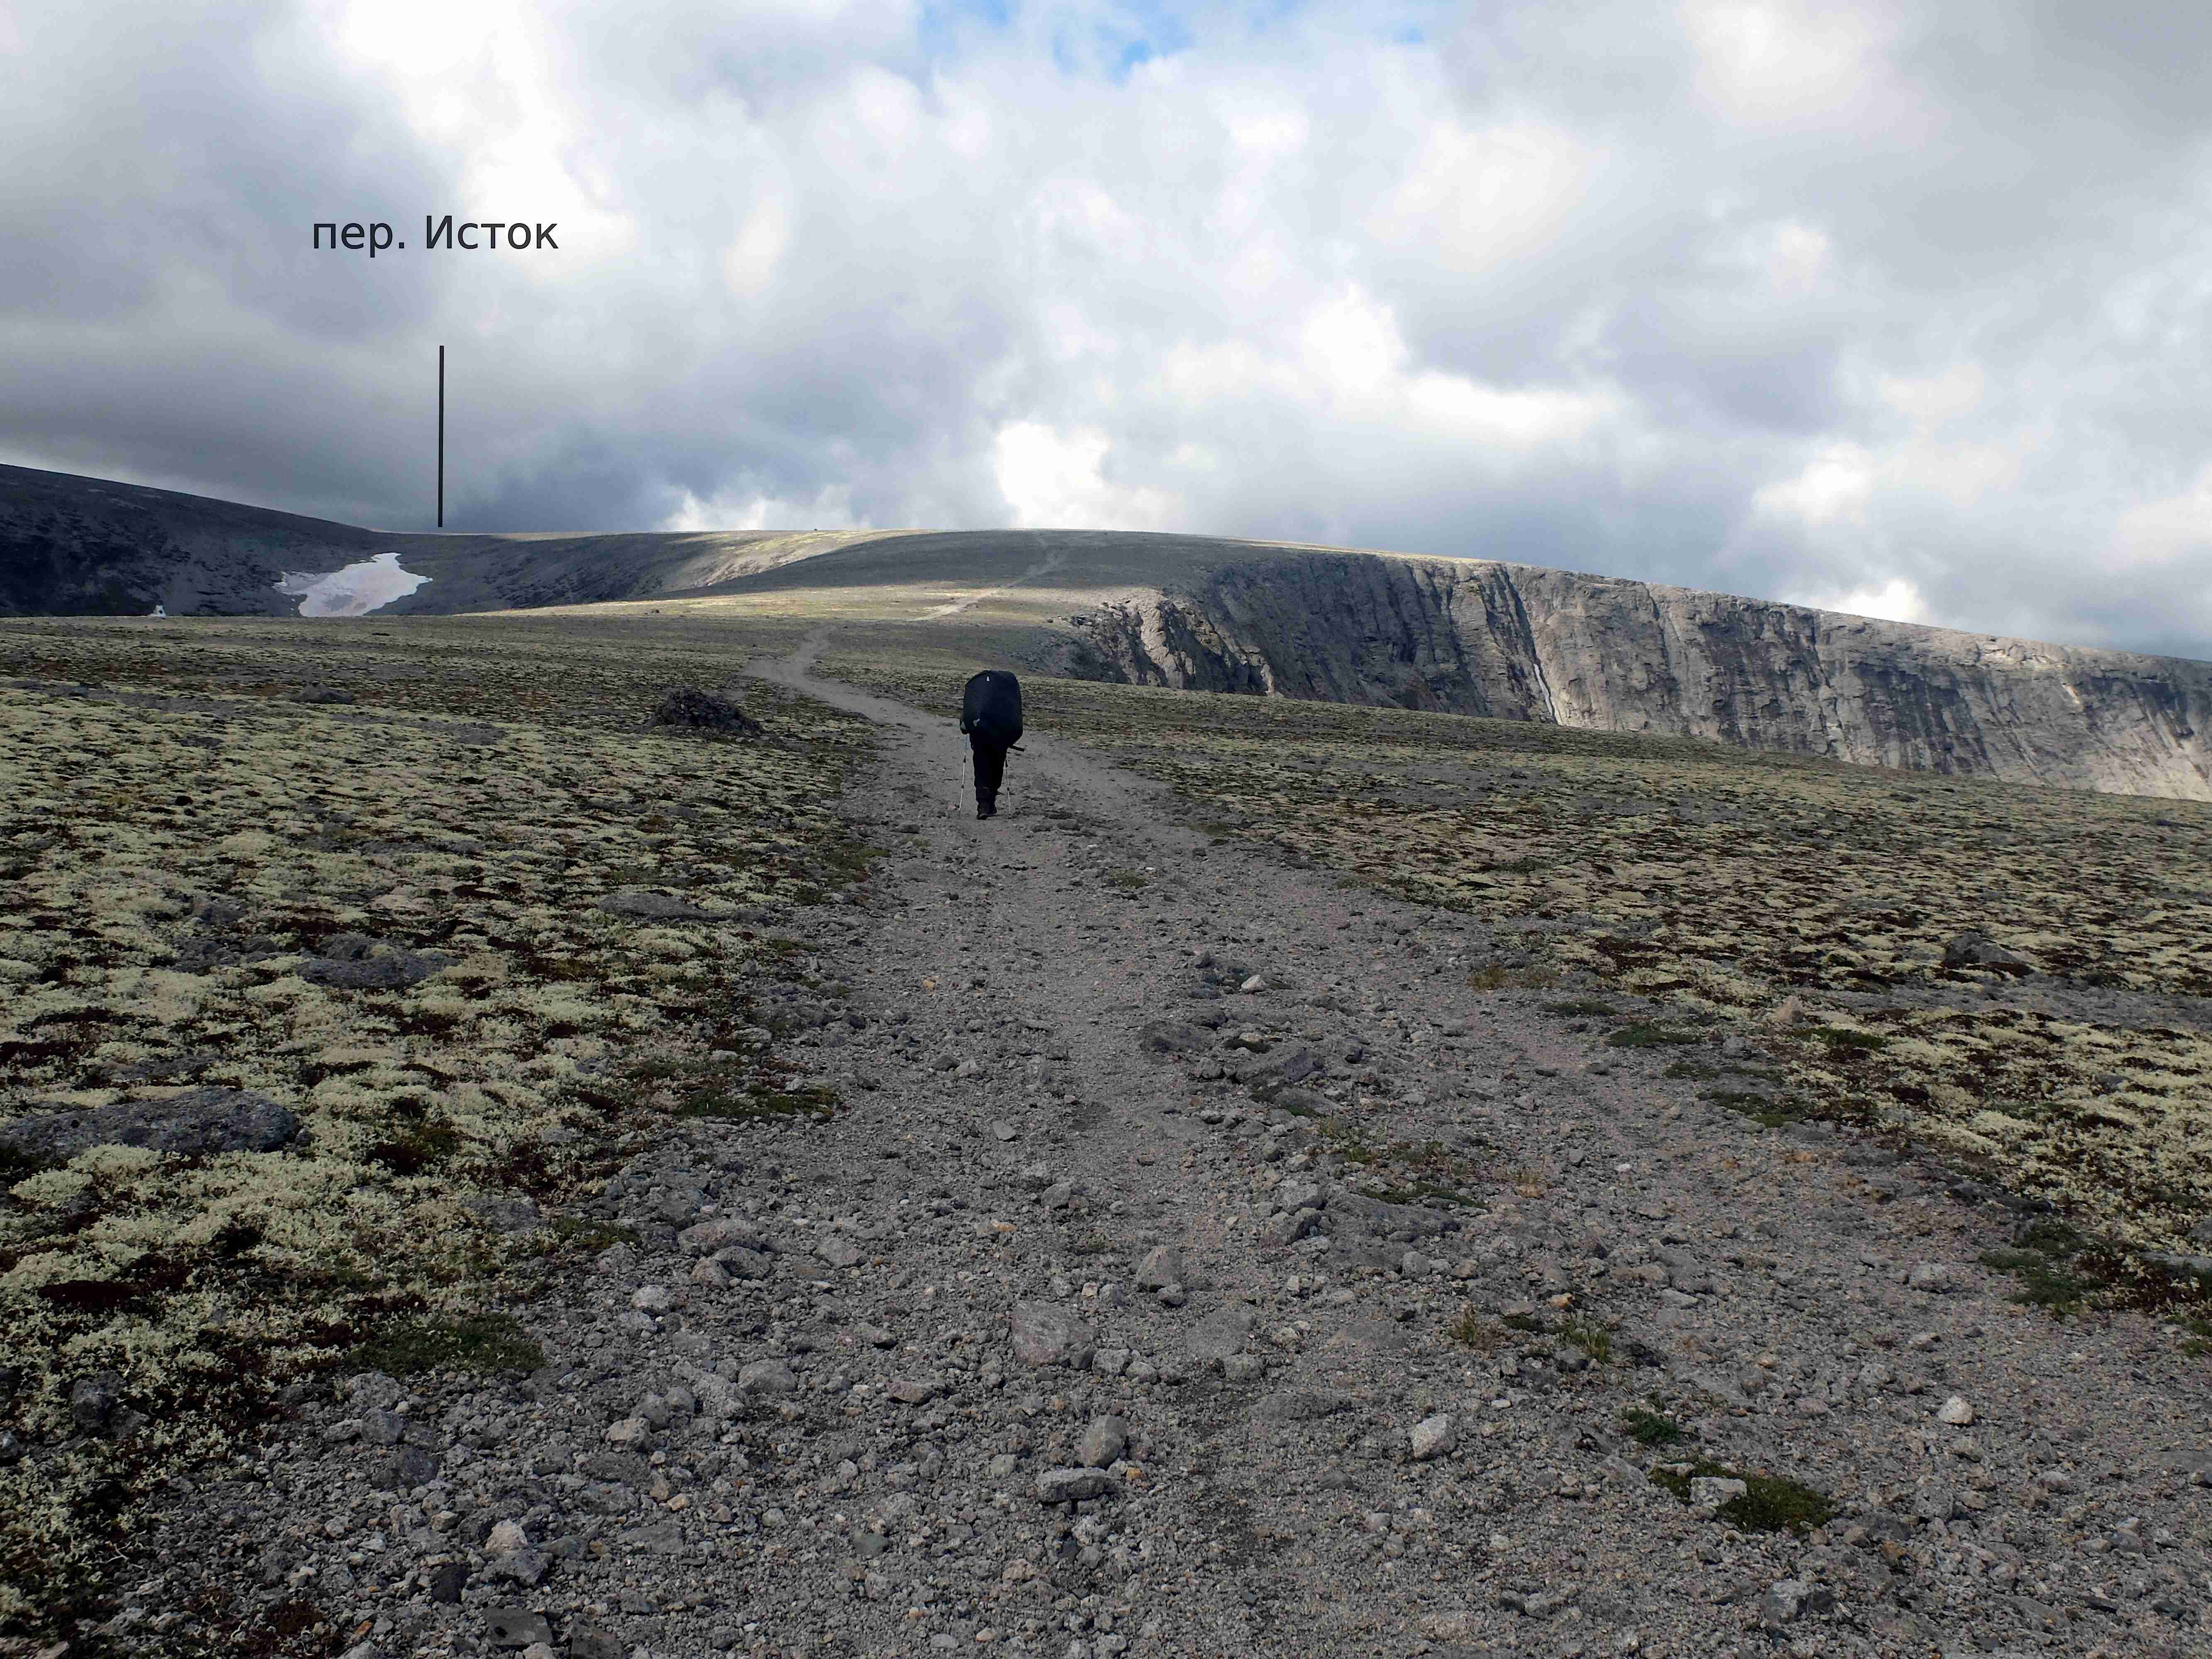
\includegraphics[width=14cm]{foto/12_08/01.К перевалу Исток.png.jpg}
    \caption{Подъём от оз. Академического к пер. Исток}
    \label{fig8:1}
\end{figure}

\begin{figure}
    \centering
    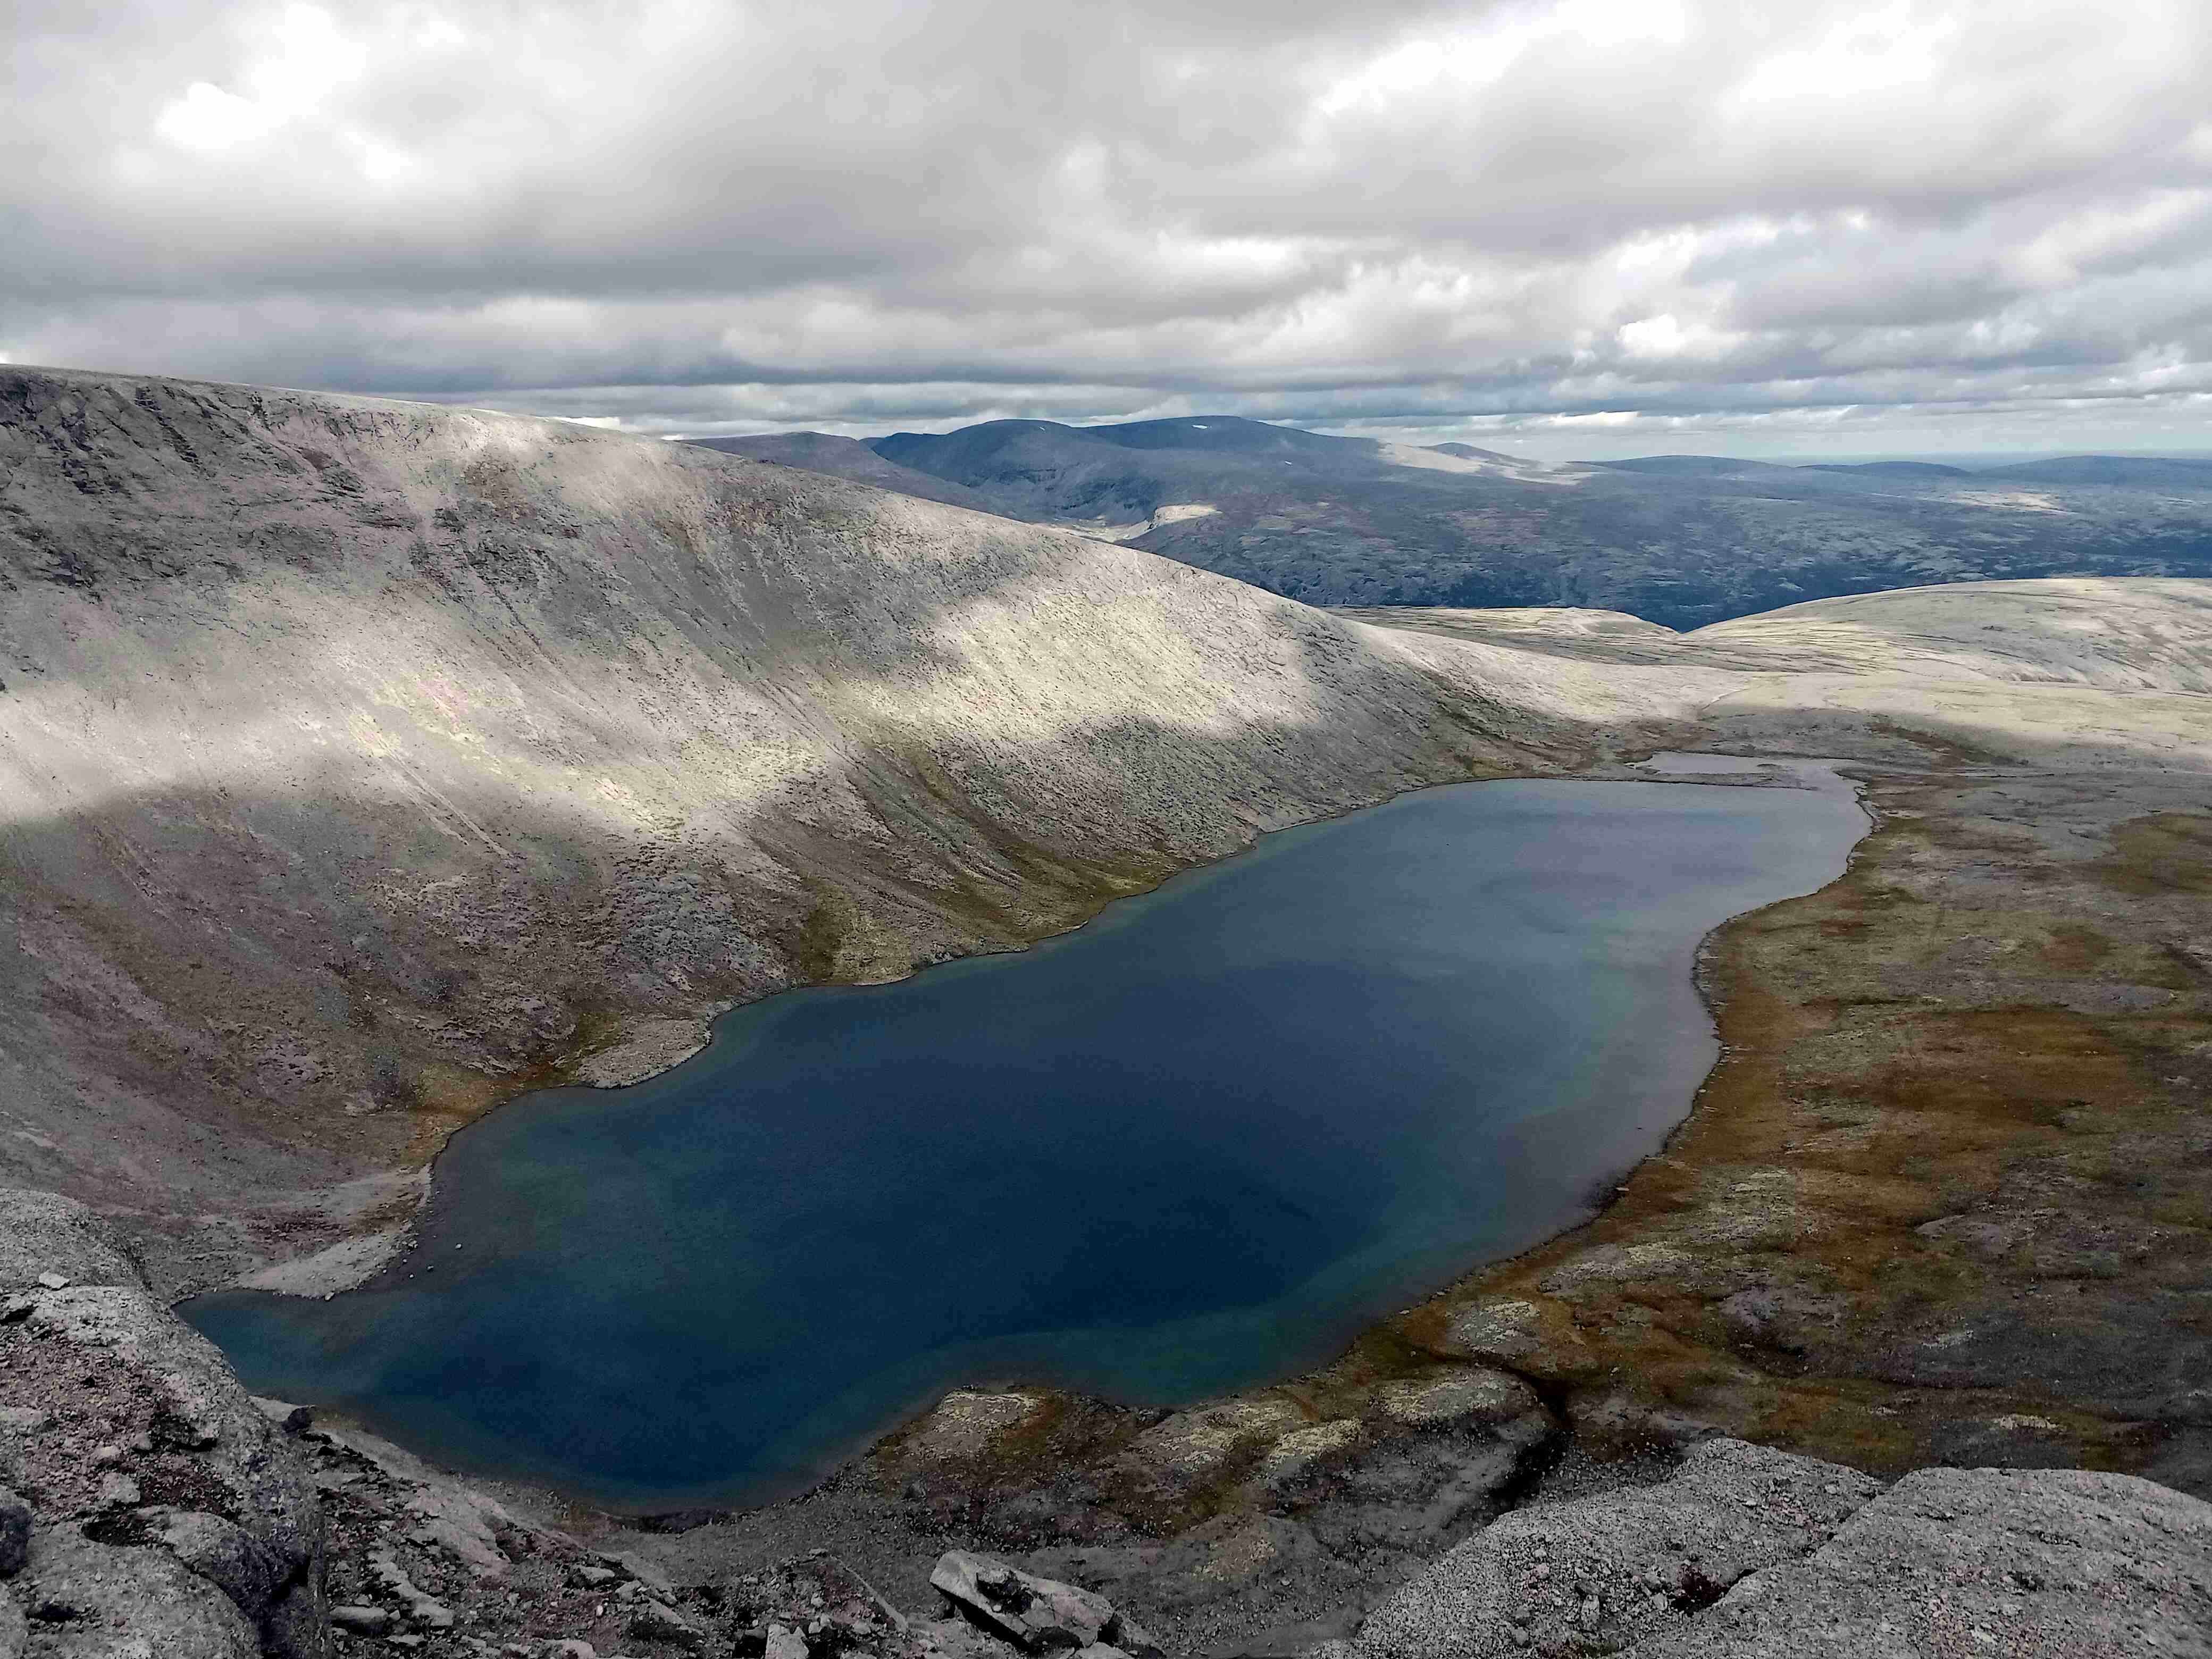
\includegraphics[width=14cm]{foto/12_08/02.Вид на озеро Академическое.png.jpg}
    \caption{Вид на оз. Академическое}
    \label{fig8:2}
\end{figure}

\begin{figure}
    \centering
    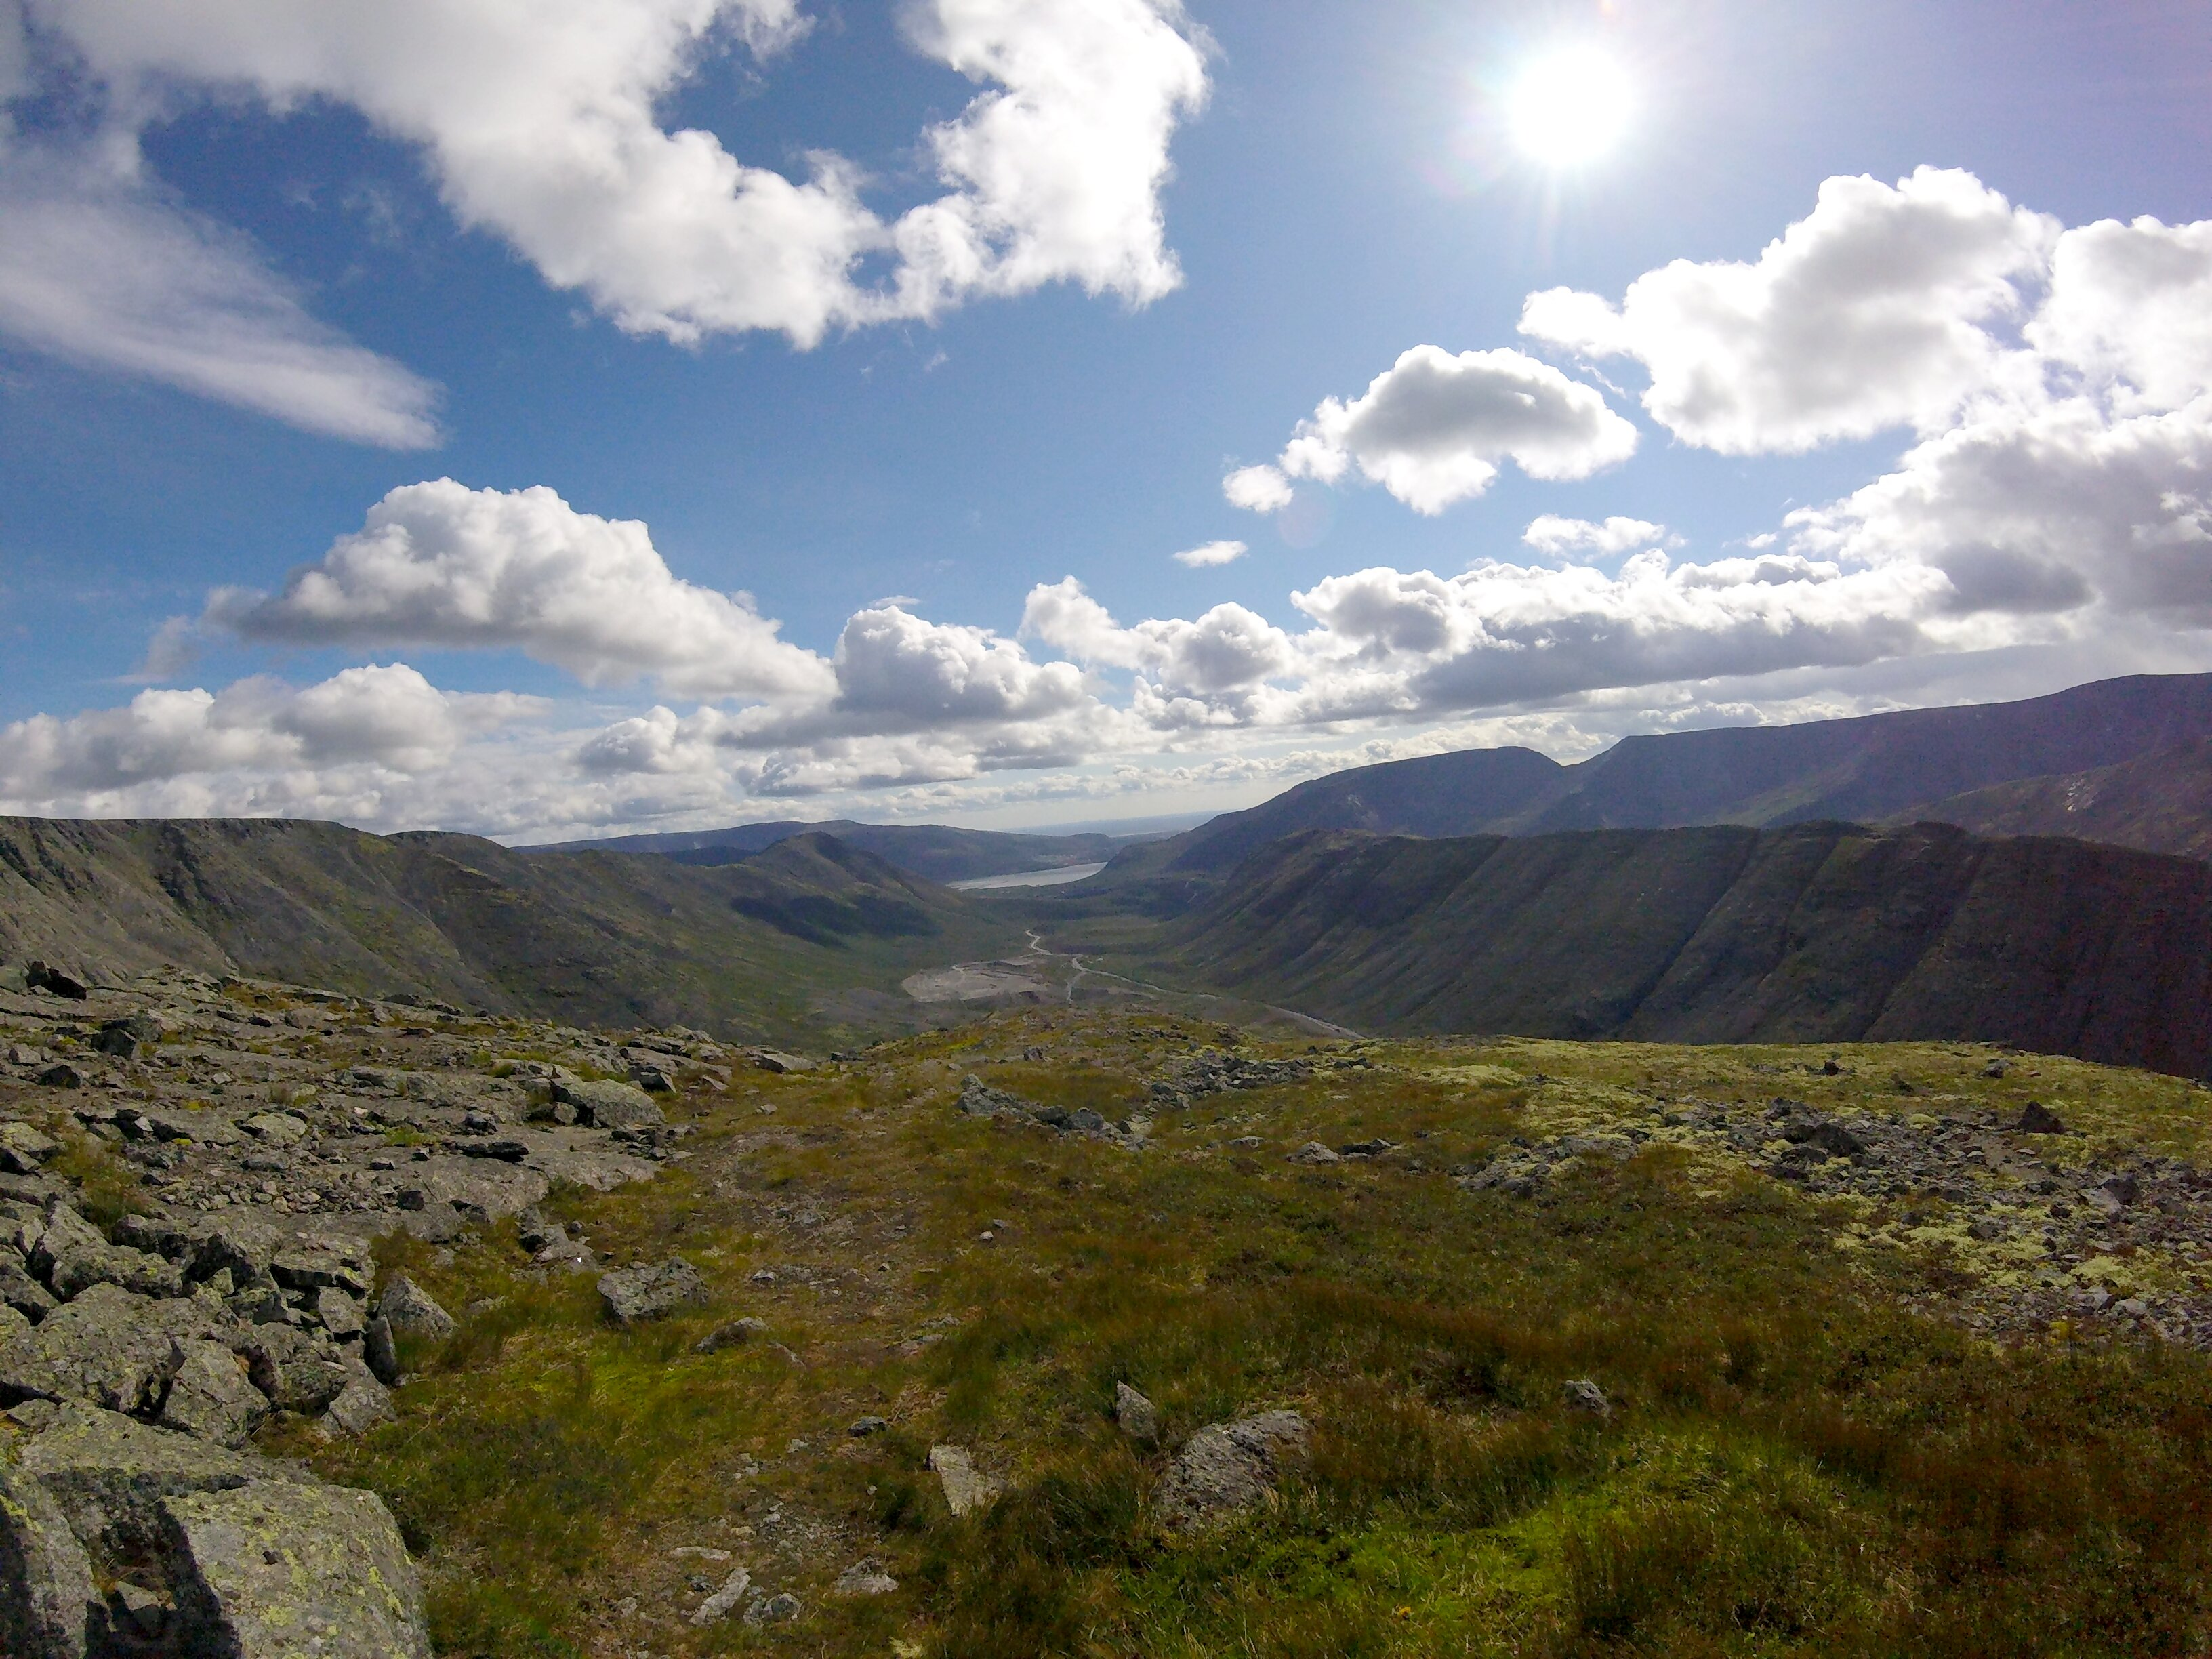
\includegraphics[width=14cm]{foto/12_08/03.Начало спуска с г.Кукисвумчорр.png.jpg}
    \caption{Начало спуска с верш. Кукисвумчорр}
    \label{fig8:3}
\end{figure}

\begin{figure}
    \centering
    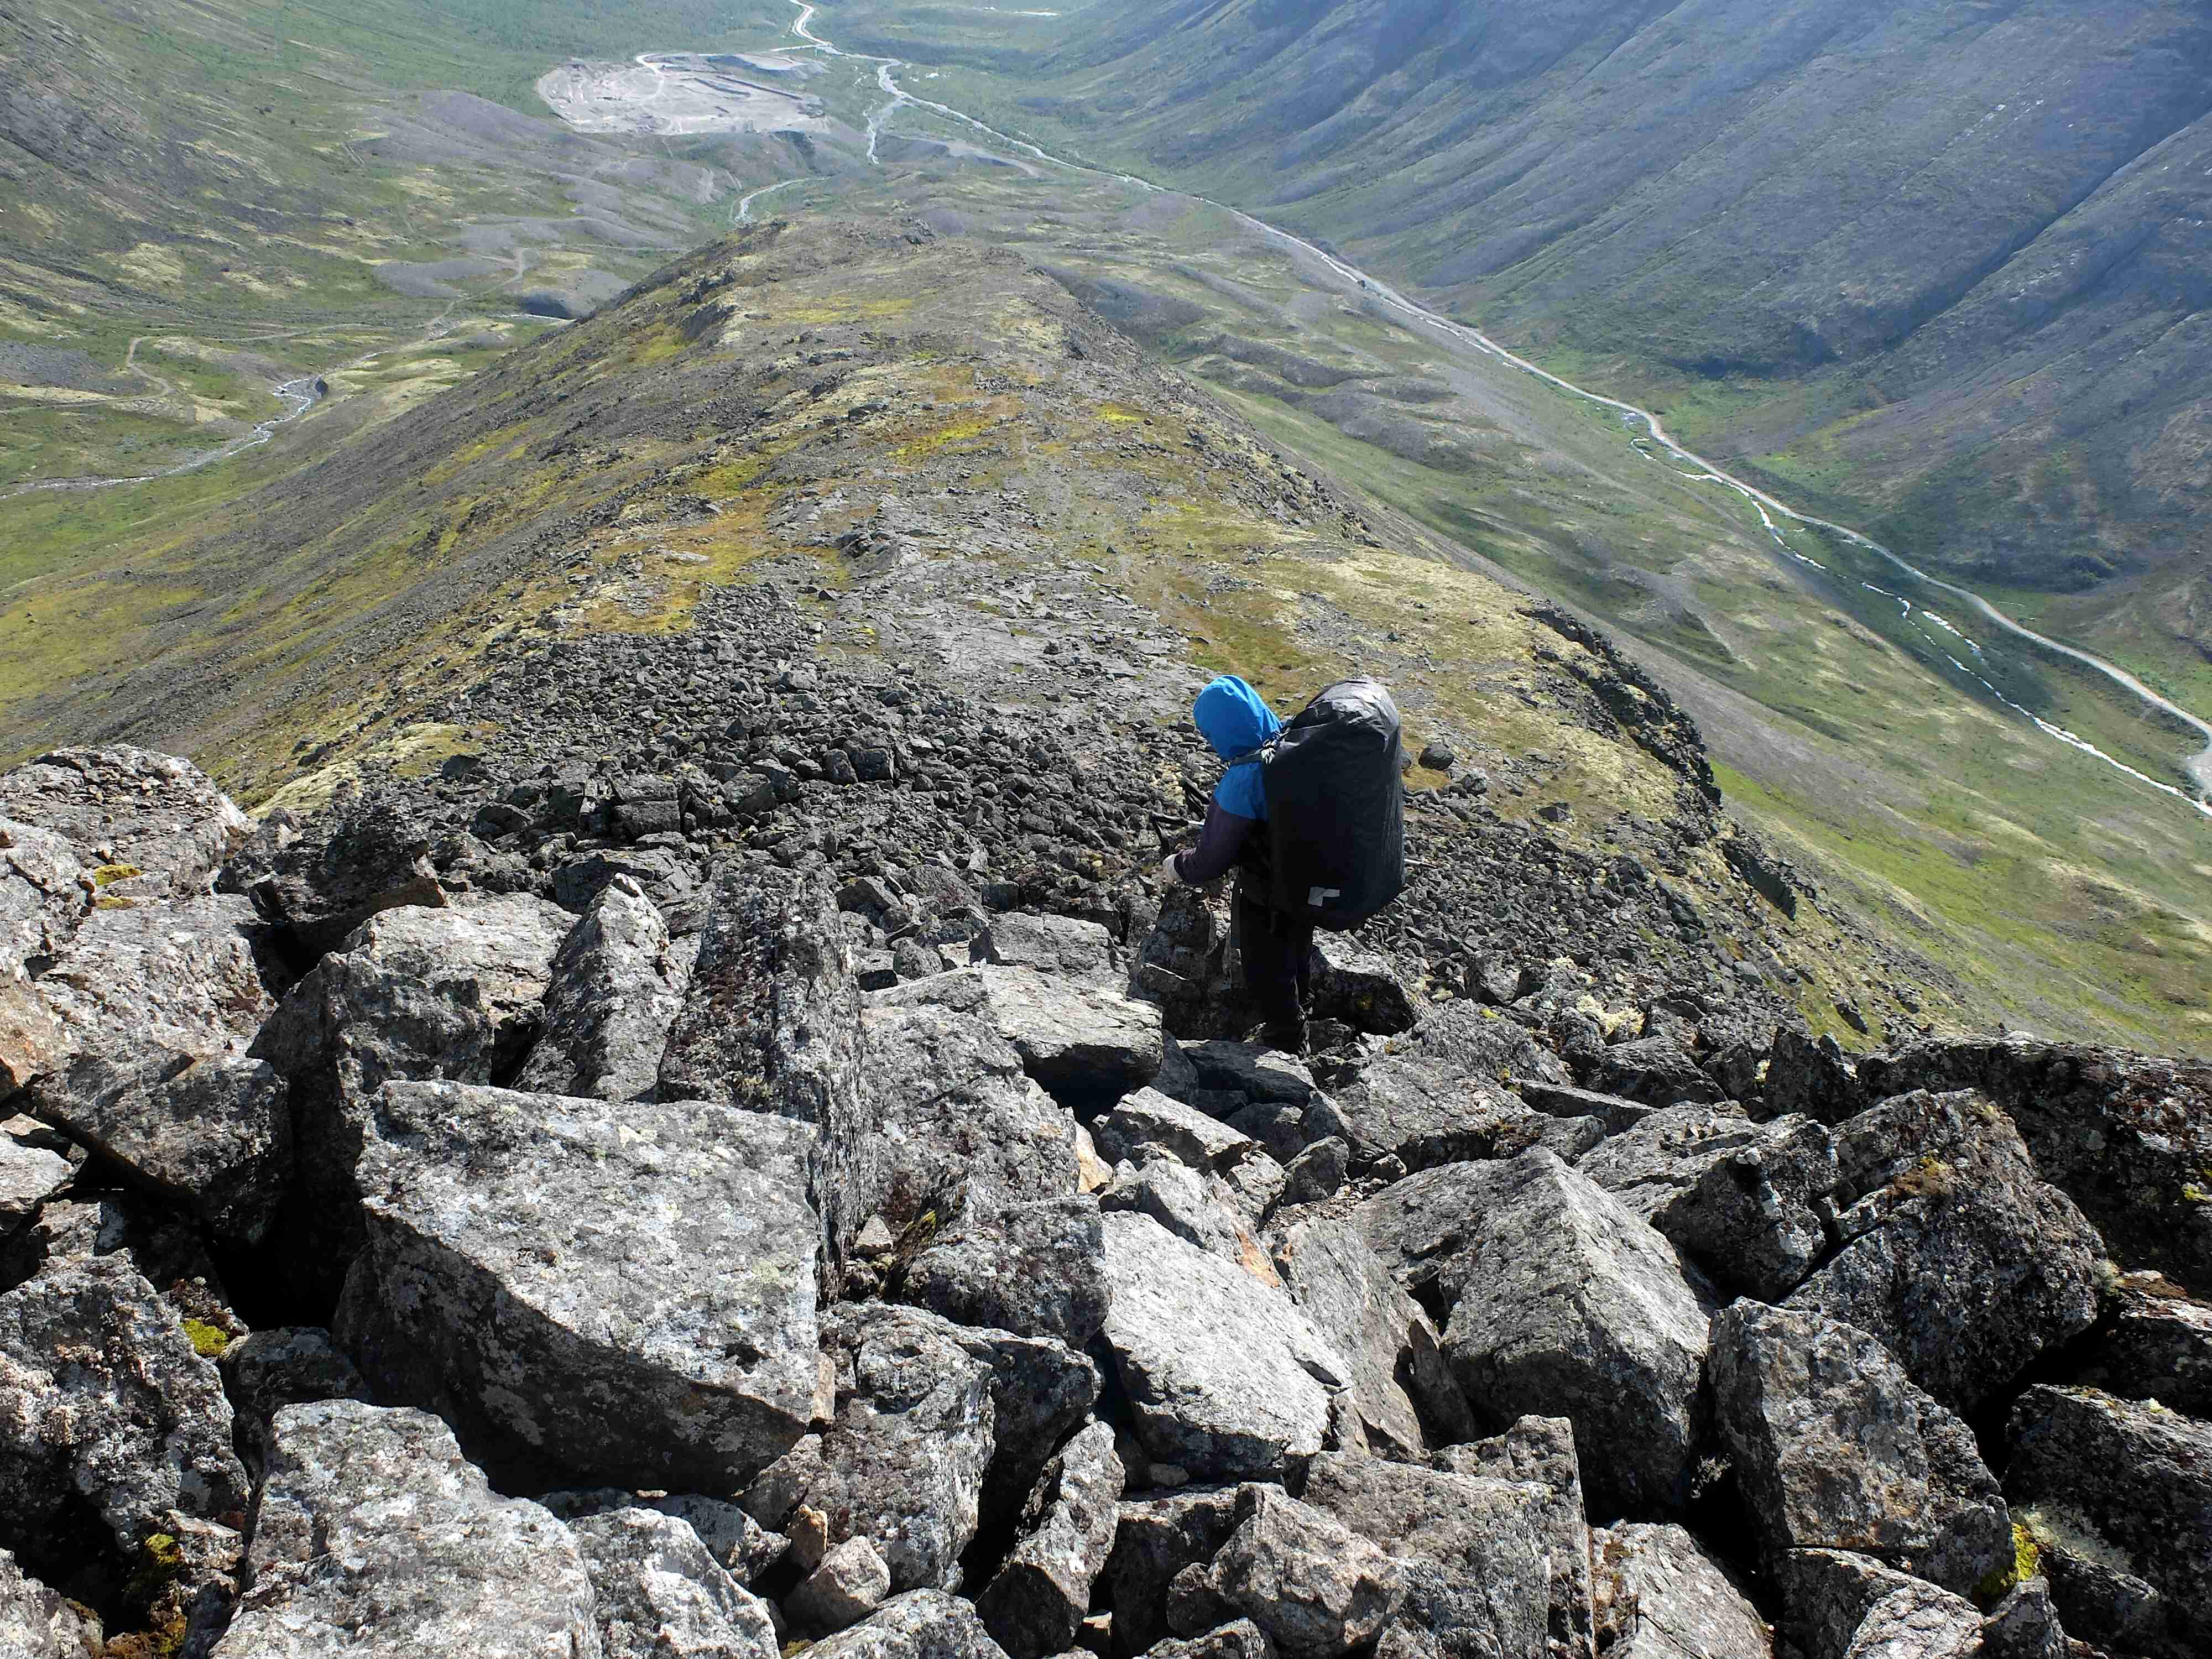
\includegraphics[width=14cm]{foto/12_08/04.Спуск по гребню.png.jpg}
    \caption{Спуск по гребню}
    \label{fig8:4}
\end{figure}

\begin{figure}
    \centering
    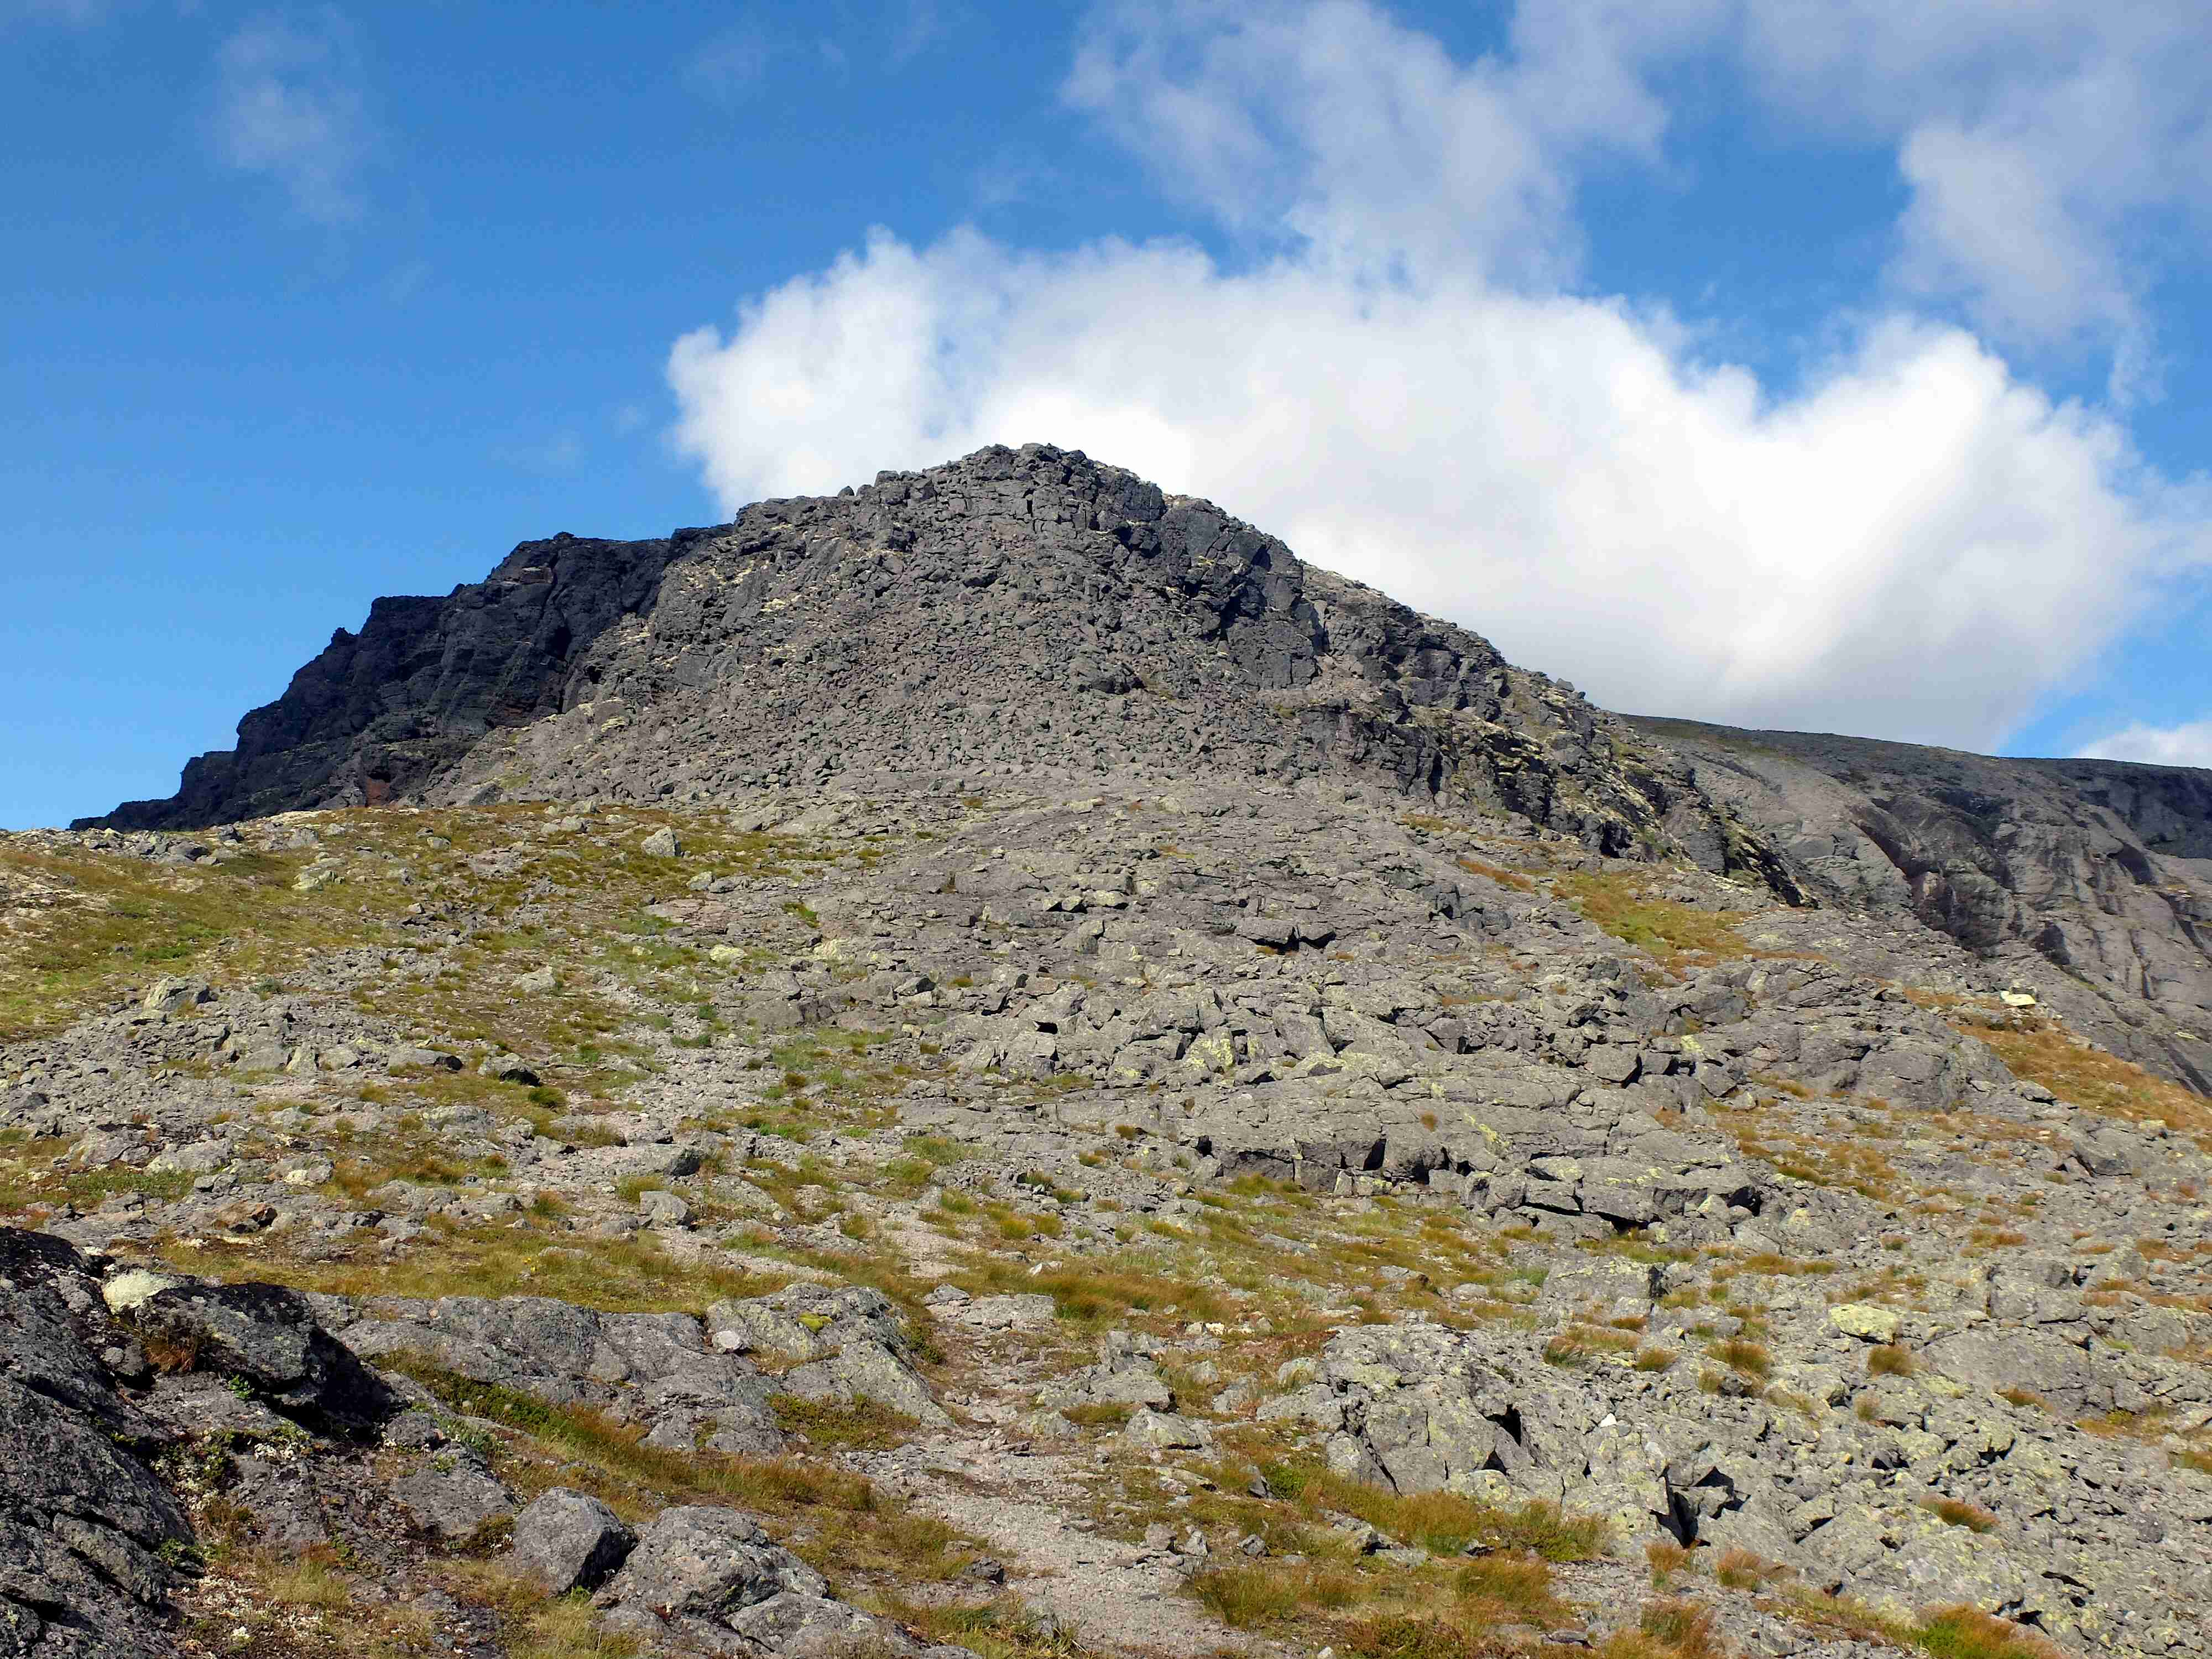
\includegraphics[width=14cm]{foto/12_08/05.Вид на гребень снизу.png.jpg}
    \caption{Вид на гребень снизу}
    \label{fig8:5}
\end{figure}

\begin{figure}
    \centering
    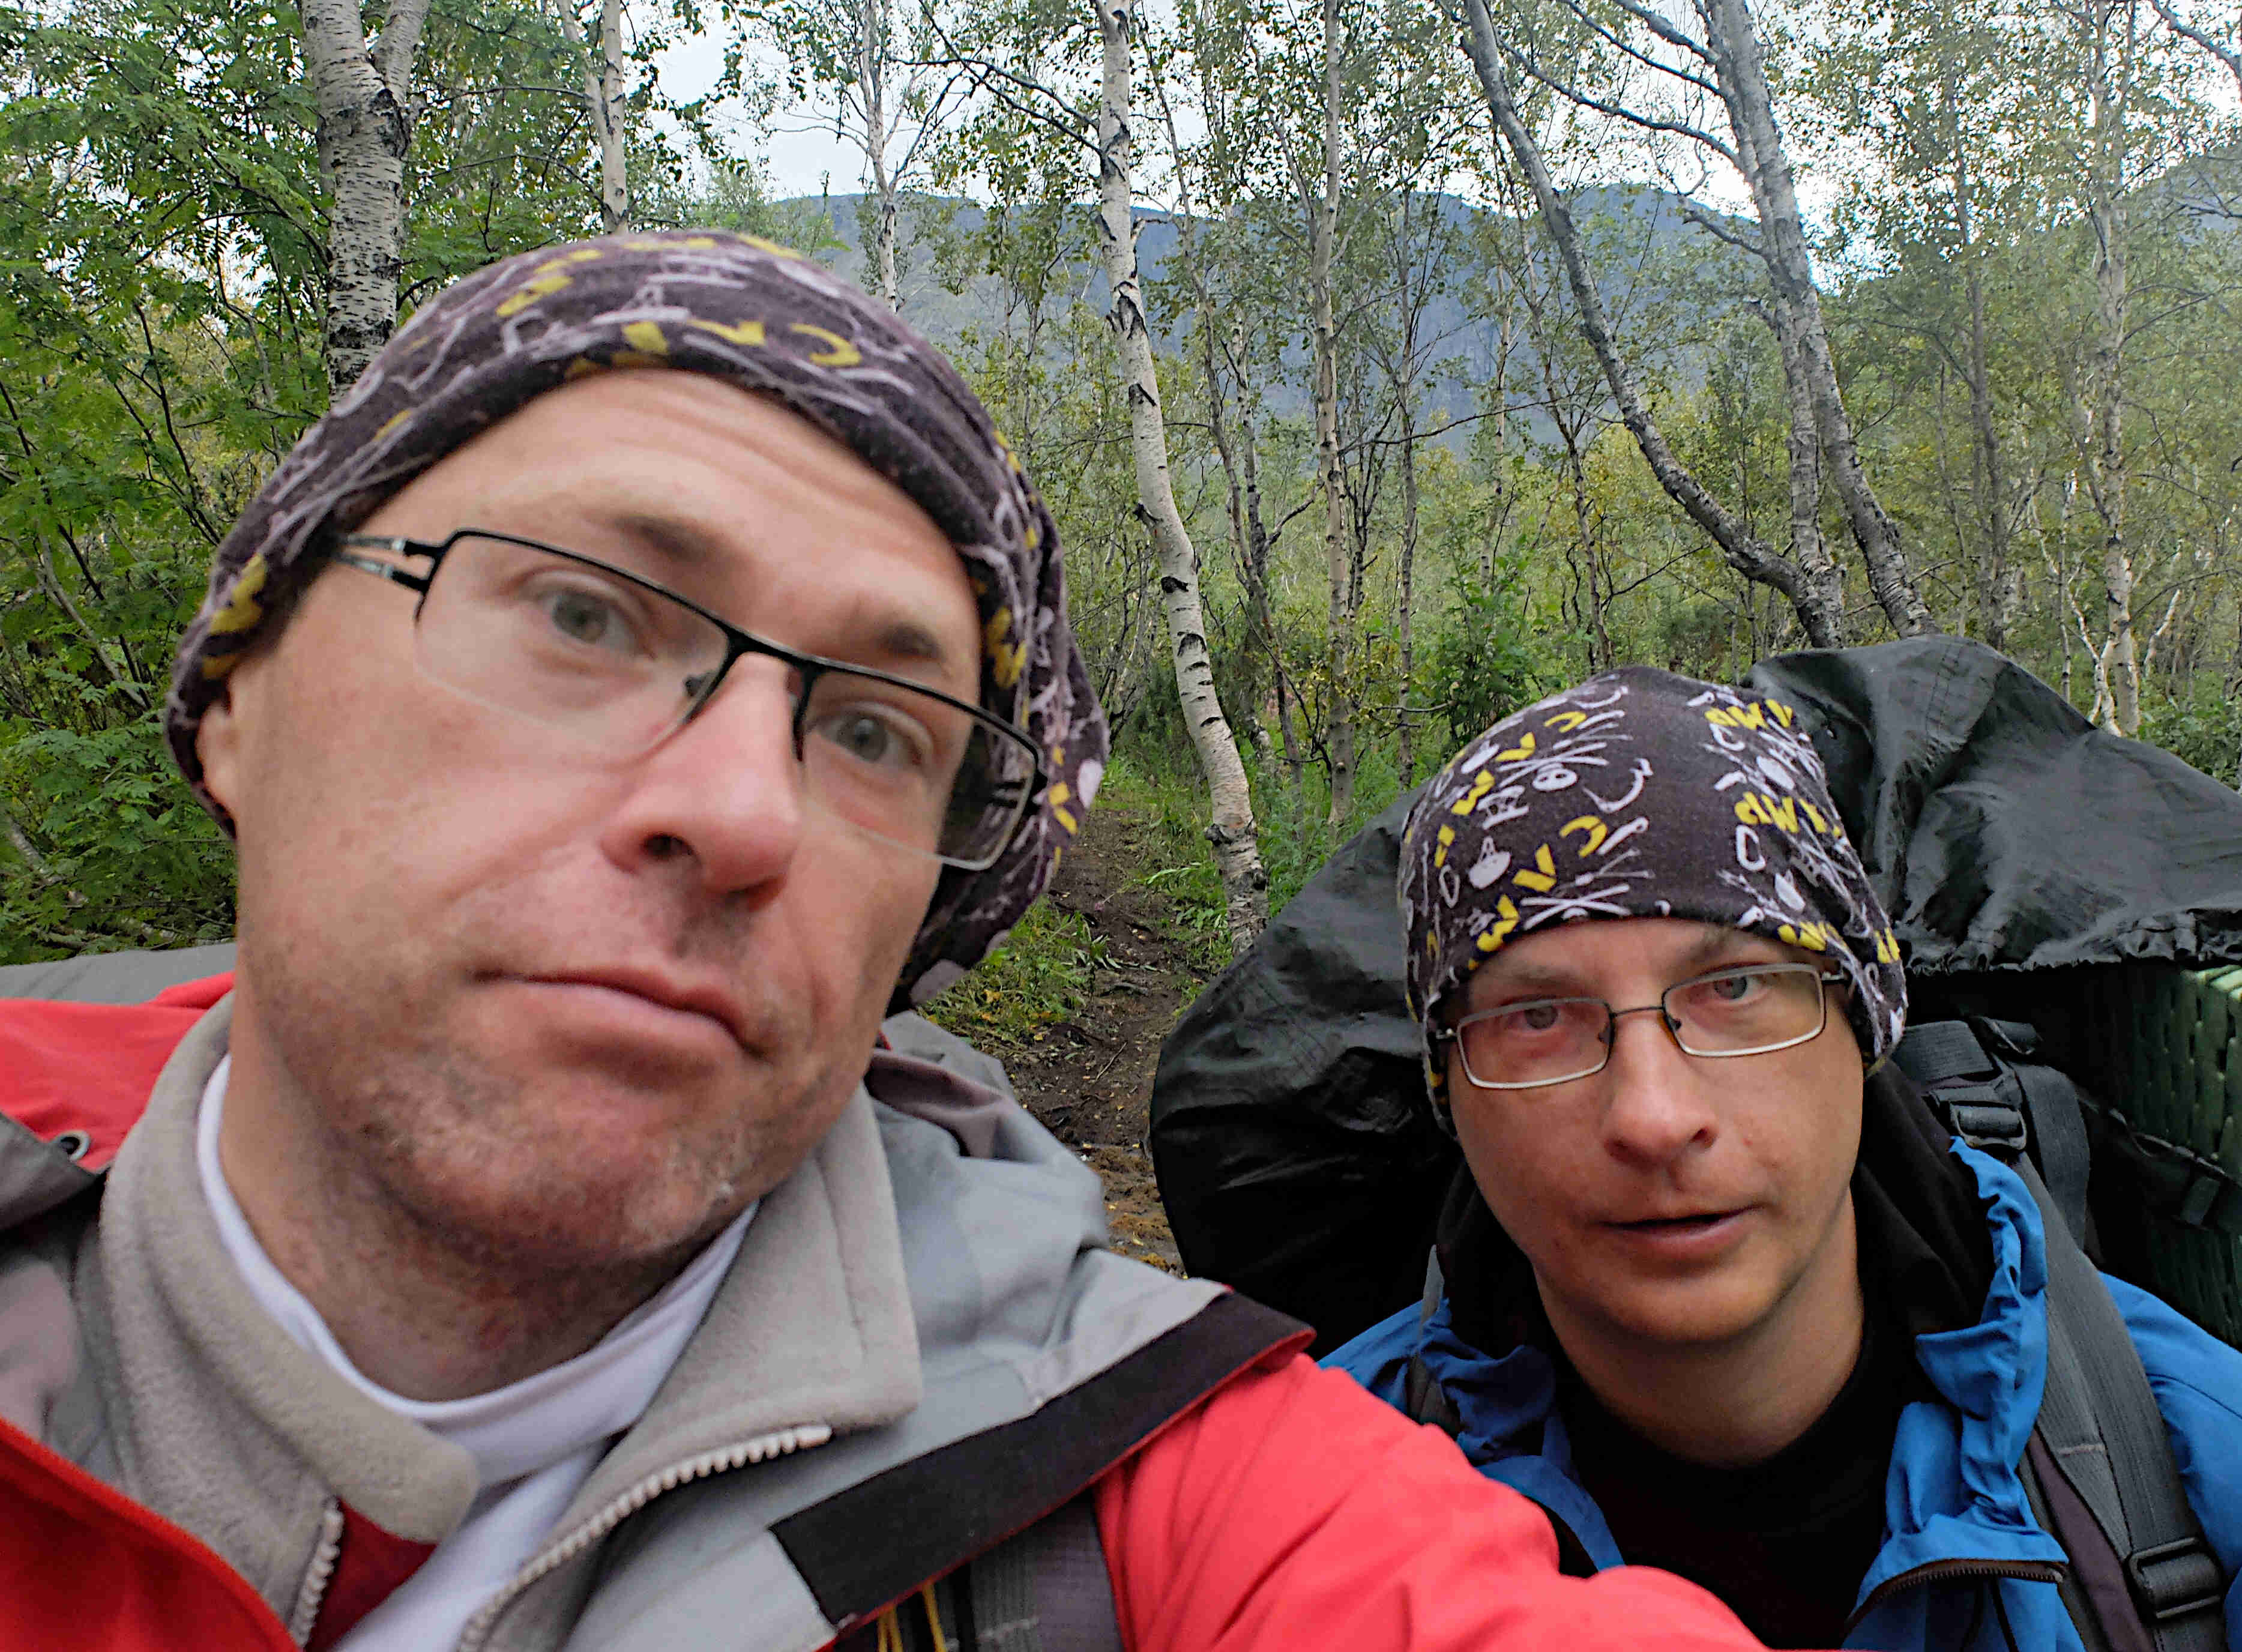
\includegraphics[width=14cm]{foto/Лица/mordas4.JPG}
    \caption{Финиш у оз. Малый Вудьявр}
    \label{fig8:6}
\end{figure}
